\documentclass[12pt,a4paper]{memoir}

%define fonts
\usepackage[utf8]{inputenc}
\usepackage[T1]{fontenc}
\usepackage[T1,OT2,T2A]{fontenc}
\usepackage[english,serbian,serbianc]{babel}
\usepackage{times} 
%\usepackage{mathptmx}
%\usepackage{mathpazo} % Use the Palatino font by default

\usepackage[dvips]{graphicx}
\usepackage{xcolor}
\usepackage{amsmath}
\usepackage{amssymb}
%\usepackage{caption}
%\usepackage{subcaption}

\usepackage[
breaklinks=true,colorlinks=true,
%linkcolor=blue,urlcolor=red,citecolor=red,% PDF VIEW
linkcolor=blue,urlcolor=red,citecolor=red,% PRINT
bookmarks=true,bookmarksopenlevel=2]{hyperref}

\usepackage[margin=20mm]{geometry}


\usepackage{multirow}
\usepackage[explicit]{titlesec}
\usepackage{setspace}
\usepackage{enumitem}
\usepackage{pdfpages}
\usepackage{ragged2e}
\usepackage[caption=false,labelformat=empty]{subfig}
\usepackage{titleps}
\usepackage{fancyhdr}
\usepackage{float}
\usepackage[bottom]{footmisc}



%\SingleSpacing
%\OnehalfSpacing
%\DoubleSpacing
%\linespread{1.3} %1.3 is onehalf spacing 
\setlength{\emergencystretch}{2.5em} %removes overfull boxes
\setlength{\parskip}{0.5em}       % Space between paragraphs (0em is default).

\raggedbottom

%%% CHAPTER'S STYLE
%\chapterstyle{bianchi}
\chapterstyle{ger}
%\chapterstyle{madsen}
%\chapterstyle{ell}
%%% STYLE OF SECTIONS, SUBSECTIONS, AND SUBSUBSECTIONS
%\setsecheadstyle{\Large\bfseries\sffamily\raggedright}
%\setsubsecheadstyle{\large\bfseries\sffamily\raggedright}
%\setsubsubsecheadstyle{\bfseries\sffamily\raggedright}
\setsecheadstyle{\centering\Large\bfseries}

%%% STYLE OF PAGES NUMBERING
%\pagestyle{companion}\nouppercaseheads 
%\pagestyle{headings}
\pagestyle{ruled}
%\pagestyle{plain}
%\makepagestyle{plain}
\makeevenfoot{ruled}{}{\thepage}{}
\makeoddfoot{ruled}{}{\thepage}{}
%\makeevenhead{plain}{}{}{}
%\makeoddhead{plain}{}{}{}
\makeevenhead{ruled}{\leftmark}{}{}
\makeoddhead{ruled}{}{}{\rightmark}


\maxsecnumdepth{subsection} % chapters, sections, and subsections are numbered
\maxtocdepth{subsection} % chapters, sections, and subsections are in the Table of Contents
%\settocdepth{section}
%\setsecnumdepth{section}
%\setcounter{secnumdepth}{1}
%%%---%%%---%%%---%%%---%%%---%%%---%%%---%%%---%%%---%%%---%%%---%%%---%%%


\graphicspath{{figs/}}
\begin{document}
\title{Evolving complex networks: structure and dynamics}

\frontmatter
%\thispagestyle{empty}
\selectlanguage{english}
\centering

\Large{
    UNIVERSITY OF BELGRADE \\
    FACULTY OF PHYSICS
}

\vspace{5.5cm}

\Large{
    Ana Vrani\' c
}

\vspace{.5cm}


\textbf{\LARGE 
  { EVOLVING COMPLEX NETWORKS: STRUCTURE AND DYNAMICS}
  }

\vspace{.5cm}

\Large{
    Doctoral Dissertation }

    \vspace{9.1cm}

\Large{
    Belgrade, 2023
}

\pagebreak
\justify
\thispagestyle{empty}


%
\selectlanguage{serbianc}
\sffamily
\fontencoding{OT2}\fontfamily{Tempora-TLF}\selectfont
\thispagestyle{empty}

\begin{center}

\Large{
    УНИВЕРЗИТЕТ У БЕОГРАДУ \\
    ФИЗИЧКИ ФАКУЛТЕТ
}

\vspace{5.5cm}

\Large{
    Aна Вранић
}

\vspace{.5cm}

\LARGE{ \textbf{
    РАСТУЋЕ КОМПЛЕКСНЕ МРЕЖЕ:\\ СТРУКТУРА И ДИНАМИКА
}}

\vspace{.5cm}

\Large{
    докторска дисертација 
    
}
\vspace{9.1cm}
\Large{
    Београд, 2023.
}
\end{center}

\selectlanguage{english}

\pagebreak
\justify
\thispagestyle{empty}


%\pagebreak

%\selectlanguage{english}
\normalsize
\pagenumbering{roman}


\chapter*{Thesis Defense Committee}

\vspace{1cm}
\begin{minipage}[t] {.45\textwidth}
	$\\$Thesis advisor: \\~\\
	\textbf{Dr. Marija Mitrović Dankulov \\}
	Associate Research Professor \\
	Institute of Physics Belgrade \\
	University of Belgrade 
	\vspace{1cm}
\end{minipage}
\hspace{\fill}
\begin{minipage}[t] {.45\textwidth}
	
%	$\\$Committee member:\\ 
%	\textbf{Prof. Dr. Sunčica Elezović Hadžić\\}
%	Professor\\
%	Faculty of Physics\\
%	University of Belgrade\\
	
%	$\\$ Committee member:\\
%	\textbf{Dr. Antun Balaž\\}
%	Research Professor\\
%	Institute of Physics Belgrade\\
%	University of Belgrade\\
	
%	$\\$Committee member:\\
%	\textbf{Dr. Svetislav Mijatović\\}
%	Professor\\
%	Faculty of Physics\\
%	University of Belgrade\vspace{1.5cm}
\end{minipage}



%\justify

%\selectlanguage{english}

\normalsize
\chapter{Acknowledgements}


This thesis was completed under the mentorship of Dr. Petar Petrović, Research Professor, at the Laboratory for Statistical Physics of Complex Systems, National Center of Excellence for the Study of Complex Systems, at the Institute of Physics Belgrade, University of Belgrade. The presented research was supported by the Ministry of Education, Science, and Technological Development of the Republic of Serbia under projects ON171017 and III43007.

Lorem ipsum dolor sit amet, consectetur adipiscing elit. In sagittis leo eu metus iaculis ultricies. Aenean consequat nibh vitae sapien tristique, eu molestie lorem placerat. Donec hendrerit enim vitae consequat pulvinar. Aenean sodales dignissim aliquam. Curabitur ut lacinia neque. Nam arcu orci, vestibulum in consectetur ac, porta a massa. Nullam rhoncus orci quis enim luctus, a bibendum lacus ultricies.

Vestibulum ut velit lectus. Maecenas tincidunt enim non nisi egestas, eu suscipit metus molestie. Pellentesque scelerisque turpis sit amet interdum iaculis. Duis id posuere nibh. Ut consequat risus eu sapien gravida, ac ultricies tellus vehicula. Suspendisse facilisis ligula id mi tristique tempor. Etiam pretium massa sed lorem interdum, ut efficitur eros sollicitudin. Vestibulum pharetra non risus et placerat. Vivamus interdum sem eu nisi mattis, et tempus lacus ornare. Nulla hendrerit, justo vitae ultrices porta, augue odio faucibus dui, luctus malesuada turpis elit non massa.

Cras pellentesque dapibus purus, et tempor odio placerat vitae. Etiam enim eros, semper sed finibus id, condimentum nec dui. Nullam non leo vitae ex accumsan luctus non mattis massa. Praesent non lectus sed est fermentum faucibus ut non sapien. In tempus condimentum tellus vel pharetra. Pellentesque vitae egestas augue. Fusce sit amet orci in mi mollis feugiat. Duis fermentum erat quis dolor tempus porttitor.

Vivamus dapibus justo metus, eu maximus massa dictum vel. Donec sed bibendum quam. Sed eleifend mi eros, in rutrum est congue ultrices. Aliquam vitae eleifend nunc, et cursus diam. Maecenas imperdiet est vel dolor commodo cursus. In venenatis metus vitae tortor ultrices, eget viverra tellus tincidunt. Lorem ipsum dolor sit amet, consectetur adipiscing elit. Vivamus quis porttitor massa, quis vehicula augue. Cras quam ipsum, placerat vel rutrum sed, pretium at velit. Aenean vel augue aliquet, gravida diam sed, dictum mi. Nam et tincidunt eros. Integer faucibus maximus odio volutpat tempor. Maecenas a orci vitae sapien pretium scelerisque. Quisque eget fermentum augue. Cras auctor vitae erat id blandit.



\hfill

\justify

%\selectlanguage{english}

\normalsize

%\chapter{Evolving complex networks: structure and dynamics}

\chapter{Abstract}

Complexity science gives us new ways to explore complex systems. Detecting the collective phenomena and understanding how they emerge from individual interactions is one of the important research problems. Complex systems are all around us; they come from physical, biological, and social systems. The complex network is a general framework for representing interaction patterns in complex systems. The structure of the network could influence the behaviour of the system. The discovery that real-world networks are far from random and show scale-free properties and small-world phenomena led to the development of this field. New theories and models were needed to study socio-economics phenomena, while statistical and computational physics tools helped analyze and model their complex network representations. %The network models are essential for understanding the rules that govern complex networks' evolution.
This thesis aims to broaden the knowledge of complex networks by empirically analyzing different online social systems and providing the models and theories that could explain their specific characteristics.  

The first part of the research explores how different growing signals influence the structure of complex networks. Over time, systems do not grow at a constant rate, and the networks that grow under fluctuating signals are clustered and correlated, while networks grown with a constant signal are not. Here we try to systematically understand the connection between the growth signal and the obtained network structure. For the growing network model, we use time series of new users from real systems, such as MySpace and TECH. At the same time, computer-generated long-range correlated signals help distinguish which properties of time series shape the structure of complex networks. When signals are correlated and have multifractal properties, they mainly influence the scale-free networks promoting the creation of highly connected nodes. 

The second part of the research focused on the evolution of large online platforms, where users organise into different kinds of social groups. These days, people interact intensively through online platforms. No matter whether the online systems rapidly grow, universal patterns in their growth stay stable. Our approach was to empirically analyse the growth of three online systems: Meetup groups in London and New York and Subreddits. Their group size distributions follow log-normal, indicating the presence of universality.
On the other hand, it was important to identify the processes that led to the emergence of log-normal distribution and provide a model that could produce growth patterns in real systems. Social connections could be an important factor in the diffusion between groups. We used a model that interplays two criteria for group choices: random and based on social connections. We showed that social interactions are more critical in Subreddits than in Meetups for the diffusion between groups. 

The last part of the research presented in the thesis addresses what is necessary for one community to be sustainable. The complex network representation of the system allows us to determine how different network properties evolve. We use data from Stack Exchange sites, comparing communities on the same topic, but one was closed, and later when the site was proposed later, it stayed active until these days. Stack Exchange sites are question and answers platforms where users share knowledge. Analyzing the structural patterns in these communities, we found active ones to be more clustered and characterized by better-connected cores. Core users are crucial for having a healthy site.
Furthermore, they need to be trustworthy. Through the dynamic reputation model, we attempt to measure the level of trust in these communities. In active communities, core users show a higher reputation than in closed communities, indicating the importance that a stable core develops early and has a high level of trust. 



\noindent
{\textbf {Keywords:}} \\ %random sequential adsorption, heterogeneous substrate, pair
%correlation function \\
{\textbf {Research field:}} Physics \\
{\textbf {Research subfield:}} Statistical physics\\
\textbf{UDC number:} 536 %539.233, 536.12

\hfill

\justify

%\normalsize


\selectlanguage{serbianc}
\sffamily
\fontencoding{OT2}\fontfamily{Tempora-TLF}\selectfont

\chapter*{{\fontencoding{OT2}\fontfamily{Tempora-TLF}\selectfont Сажетак}}
\thispagestyle{empty} 

Комплексни системи се налазе свуда око нас у различитим доменима физике, биологије и друштвених наука. Иако се разликују по пореклу и функцији, заједничка карактеристика им је да се састоје од великог броја елемената који међусобно интерагују и због тих интеракција испоњавају колективно понашање. Комплексне мреже представљају општи приступ за репрезентацију образаца интеракција у комплексним системима. Структура комплексне мреже и њена еволуција су узајамно повезане са динамиком и функцијом комплексног система. Проналажење колективних фенома и разумевање како они настају из индивидуалних интеракција је један од важних истраживачких проблема. Теорија комплексних система нам пружа нове методе за истраживање комплексних система. Она комбинује методе статистичке физике, рачунарске физике, теорије комплексних мрежа, компјутерских наука како би квантитативно описала и проучавала различите колективне појаве и предложила теоријске моделе ради бољег разумевања механизама који су у основи динамике и еволуције комплексних мрежа. 

Ова теза има за циљ да прошири знање о структури и динамици растућих комплексних мрежа кроз анализу емпиријских података из различитих онлајн друштвених система и дефинисањем модела и теорија које би могле да објасне њихове специфичне карактеристике. Друштвени системи стално еволуирају и због тога је неопходно разумети везе између њихове структуре, раста и сегментације и како те везе утичу на њихову одрживост.

Ранији радови сугерисали су да својства сигнала раста утичу на структуру и динамику растућих комплексних мрежа. У реалним онлајн системима, сигнали раста флуктуирају током времена и они су дугодометно корелисани и имају мултифрактална својства. Као сигнале раста у овој тези, користимо временске серије нових корисника из реалних система {\selectlanguage{english}MySpace} и {\selectlanguage{english}TECH}, и компјутерски генерисане сигнале са специфичним својствима дугодометних корелација. Комбинујемо их са мрежним моделом старости чворова да бисмо детаљно испитали како карактеристике ових сигнала утичу на структуру комплесних мрежа. Наши резултати показују да својства сигнала раста имају најзначајнији утицај на структуру мрежа са широким степеном дистрибуције. За разлику од мрежа које имају константан раст, ове мреже су кластерисане и корелиране.

Даље, истражујемо како сигнал раста и правила повезивања утичу на сегментацију и раст социјалних група. Емпиријска анализа различитих друштвено-економских система указује на то да упркос разликама, ови системи често испољавају нека универзална својства у погледу сегментације и раста. Проучавали смо {\selectlanguage{english}Meetup} групе настале у Лондону и Њујорку, као и {\selectlanguage{english}subReddit} и открили да је дистрибуција величине група у овим системима логнормална и универзална током времена, локације и теме групе. Користили смо модел који комбинује два критеријума за повезивање корисника са друштвеним групама, насумично и на онову друштвених веза. Показали смо да су друштвене интеракције битан фактор при настанку логнормалне дистрибуције. Механизми под којима се корисници придружују друштвеним групама могу објаснити појаву универзалних својстава у друштвеном систему.

Комплексна теорија мрежа нам омогућава да опишемо како се развијају различита својства мреже и разумемо како еволуција утиче на њихову одрживост. Користили смо податке са {\selectlanguage{english}Stack Exchange} сајтова и упоређивали еволуцију структуре мреже за парове активних и затворених заједница током њихове ране фазе постојања. {\selectlanguage{english}Stack Exchange} сајтови су платформа за питања и одговоре на којима корисници деле знање о некој специфичној теми. Упоредили смо активне и затворене заједнице на четири теме, а то су астрономија, књижевност, економија и физика. Анализирали смо структурне обрасце у овим заједницама и открили да су активне више кластерисане и да их карактерише боље повезана и стабилност језгра. 
%Основни корисници су кључни за здрав сајт и морају да буду поуздани. 
Кроз динамички модел репутације измерили смо ниво поверења у овим заједницама. У активним заједницама, корисници који се налазе у језгру имају већу репутацију него у затвореним заједницама, што указује на важност да се стабилно језгро развије рано и да има висок ниво поверења.

\noindent
\textbf{Кључне речи:} статистичка физика комплексних система, структура и динамика комплексних мрежа, моделовање онлајн социјалних система \\
%{\textbf {Keywords:}} statistical physics of complex systems,  the structure and dynamics of complex networks, modeling online social systems \\%случајна секвенцијална адсорпција, хетерогени супстрати,
%парна корелациона функција\\
\textbf{Научна област:} Физика \\
\textbf{Ужа научна област:} Статистичка физика \\
\textbf{УДК број:} 536 %539.233, 536.12

\selectlanguage{english}

%\pagebreak

%\selectlanguage{english}

\tableofcontents

\hfill

%\selectlanguage{english}
\normalsize


\def\listfigurename{List of figures}
\listoffigures

\hfill
\justify

%\selectlanguage{english}

\listoftables



\mainmatter
\selectlanguage{english}
%\chapter{Introduction} % Main chapter title
%\selectlanguage{serbianc}
%\sffamily
%\fontencoding{OT2}\fontfamily{Tempora-TLF}\selectfont

%TODO-OK prvi paragraf Prvi paragraf: -uvod u to sta su kompleksni sistemi (kolektivno ponasanje, primeri…) do na ispravke, taj prvi paragraf je isti kao u trenutnoj verziji

%TODO drugi Drugi paragraf: Kompleksne mreze – kompleksni sistemi mogu da se predstave kompleksnim mrezama gde su elenti cvorovi a interkacije linkovi. Stuktura ovih mreza je netrivijalna.  Cetvrti moze da posluzi kao opis mapiranja. A trenutna verzija treceg paragrafa do na prvu recenicu moze da se iskoristi lepo za primere.

%TODO treci paragraf Treci paragraf: Struktura je direktno vezana za dinamiku I funkciju. Pre svega se fokusirati na primere. 

%TODO cetvrti paragraf Cetvrti paragraf: Pocnes recenicom iz treceg paragrafa “The interactions between the complex system elements are not homogeneous; as systems evolve, they can also change [2].” I ovde pises malo o evoluciji mreza (primeri), ona utice na dinamiku I dinamika utice na nju. 

%TODO Peti je Universality: Mozda jednu recenicu o univerzalnosti u fizici. 

%TODO sesti Sesti paragraf: Socijalni sistemi i socijalne mreze. Zasto je proucavanje mreza bitno, sociofizika. I najbitnije, socijalni sistemi su vrlo dinamicni (broj elemenata, broj linkova I struktura mreze se menjaju), mreze konstantno evoluiraju. Sa druge strane uprkos vrlo dinamicnoj slici, postoje neke univerzalne osobine kako za dinamiku sistema, tako I za strukturu mreze. Stoga je razumevanje strukture I dinamike rastucih kompleksnih mreza. U ovoj tezi cemo se baviti strukturom I dinamikom socijalnih mreza.   

%TODO sedmi paragraf: Sedmi Paragraf o statistickoj fizici kompleksnih mreza + teorija kompleksnih mreza 

Many real systems, such as brain networks, social organisations, cities or cells, consist of many interacting units and belong to a class commonly known as complex systems. One of the most prominent characteristics of complex systems is that they exhibit emergent collective behaviour that can not be predicted based on the behaviour of individual components. The interactions between system components can be represented as a complex network \cite{kwapien2012}. The emergence of collective behaviour strongly depends on the structure of the network of interactions. The structure of the brain network and its properties are fundamental for brain functioning, while an emergent phenomenon is a human intelligence. In societies, people's interactions lead to civilisation, economy, formation of social groups. Also, the animal populations show different levels of organisation: such as patterns in bird flocks or schools of fish \cite{thurner2018}.

Despite the differences between complex systems, they can be studied using the same techniques. The natural extension of the complex system is the network, which consists of sets of nodes (vertices) and links (edges). Elements in the system are nodes, while interactions between them are given as edges. This approximation allows us to treat equally social \cite{myers2014, sarigol2014} (graph of actors), biological (network of proteins) \cite{fraiman2009ising, schneider2011modeling} or even technological systems (internet, traffic) \cite{costa2007characterization, costa2011analyzing, newman2003structure}. The research in complex systems mainly focuses on the interactions between its units. Knowing the shape of these connections, we can determine the properties of the system \cite{ladyman2013}. We can construct a representation with neurons and synapses representing connectivity in the brain network. Neurons in the same brain area are closely connected \cite{latora2017complex}. Similarly, we can define communication between people. The structure of these interactions gives us insights, for example, how information propagates through the system. The presence of people with many connections can lead to faster information flow. 

While the relationships between individuals characterise the structure of complex networks, the dynamics are related to the changes in individual behaviours over time. As real complex networks constantly evolve, the interactions between their elements can also change \cite{thurner2018}. Networks can exhibit addition of new nodes, removal of existing nodes, or changing connection strength between nodes. While these changes occur, the structure, but also the function of the network could be affected. The formation of clusters, hubs, and node removal directly influence network connectivity and robustness. 

The application of principles of statistical physics and complex network theory in the study of social systems lead to the creation of the new, interdisciplinary field of socio-physics \cite{sen2014sociophysics}. It provides methods for the statistical description of the structure and dynamics of social networks. Social networks are very dynamic, and despite their constant evolution, they show universal properties \cite{schweitzer2018sociophysics}.

Broadly, universality is an important property of complex systems \cite{binney1992}. One of the well-known examples of universality in physics is phase transition, where a system changes its state, such as in Ising model of magnetization \cite{sethna2021statistical}. At a critical transition point, the system's state is independent of interactions between spins and the lattice configuration. In systems where elements are ordered randomly, as is the case in complex networks, we also find universal behaviour. For example, the time lap between two email messages follows the power-law distribution \cite{garas2012emotional}, and the exponent is universal across different platforms. Similar conclusions are found in distributions of the votes in elections \cite{fortunato2007scaling, chatterjee2013}, and citations of scientific publications \cite{radicchi2008}. Even the growth of social groups, such as cities, follows universal patterns. The probability distribution of the city sizes in one country follows the same laws, with a similar exponent for all countries \cite{barthelemy2019, fazio2015pareto}. However, the distribution of company sizes follows log-normal behaviour and remains stable over decades \cite{amaral1997scaling, stanley1996scaling}. Identifying universal behaviour and understanding its emergence in the system is one of the focuses in the statistical physics of complex networks \cite{verbavatz2020}. Although, in this thesis we will explore the structural and dynamical properties of evolving online social networks and apply complex network models.  

When constructing complex network models, the specific mechanisms that govern social interaction and lead to observed macroscopic properties in empirical networks must be considered \cite{sen2014sociophysics}. Many studies confirmed that networks show power-law scaling in the distribution of the number of connections, high clustering, and nodes tend to connect to structurally similar nodes. For that reason, complex network models have been created to mimic properties found in real social systems \cite{sen2014sociophysics}.

The complex network theory originates from the graph theory in mathematics. The first problem solved using graph theory was the $Konigsberg$ problem of seven bridges. The city of $Konigsberg$ had seven bridges connecting the city's parts across the river and the island in the middle. Is it possible to find a walk that crosses all seven bridges only once? Representing the problem as a graph, Euler managed to simplify the problem; the parts of the land are represented as nodes while bridges between them are links, see Figure \ref{fig:Krgraph}. Crossing each bridge only once is possible if each part of the land has an even number of connections. It makes it possible to enter one part of the land from one bridge and leave it on the other. As each node has an odd number of connections, it is impossible; see Figure. \ref{fig:Krgraph}.

\begin{figure}[!ht]
	\centering
	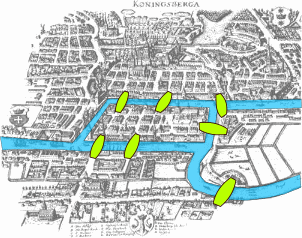
\includegraphics[width=0.3\linewidth]{chapter1/Konigsberg_bridges.png} \hspace{2cm}
	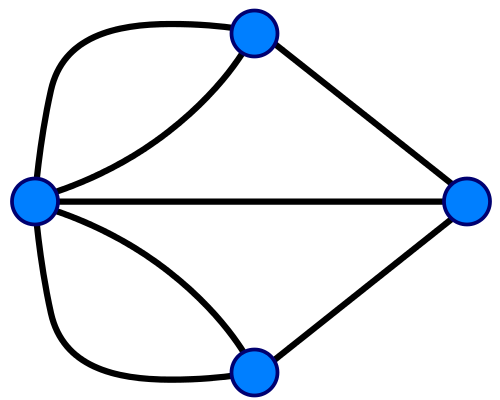
\includegraphics[width=0.3\linewidth]{chapter1/Konigsberg_graph.png}
	\caption[\selectlanguage{english}Konigsberg problem of seven bridges.]{The Kronigsber problem of seven bridges. The left panel shows the original map of the bridges; the right panel shows its graph representation. }
	
	\label{fig:Krgraph}
\end{figure}

Until the late 1990s, graph theory was not widely used. Back then, the most crucial model was the Erdos-Reni model of random graphs, which considers a fixed number of nodes in the network connected randomly, resulting in the Poisson degree distribution. When researchers got an idea to map the World Wide Web (WWW) on the network and analyse its properties \cite{huberman1999}, they found that degree distribution follows the power-law contrary to expected behaviour from random graph model \cite{dorogovtsev2010complex}. Because the power-law distribution is the same on all scales, such networks are called scale-free. Besides the scale-free property, empirical analysis of various complex networks showed the small-world property, and the high clustering coefficient \cite{barabasi2009,newman2010}. Two seminal papers from 1999 inspired further research in complex networks. Watts and Strogatz \cite{watts1998collective} proposed the model where rewiring of edges on regular lattice leads to the network in which paths between any two nodes become small (small-world) and nodes become densely connected, resulting in a high clustering coefficient. On the other hand, Barabasi and Albert (BA) \cite{barabasi1999} introduced the model, where the network grows over time, and the new nodes tend to connect high-degree nodes; it produces scale-free networks with few highly connected nodes. 

Different complex network models were proposed to describe the structure and dynamics of social and technological systems. The node degree is one of many node features that determine the linking probability, and the linking probability may be nonlinear in node degree or may depend on the age of the node \cite{dorogovtsev2000b, dorogovtsev2001b}. In the BA model, the links are introduced through new nodes, so it was proposed that links can be created between existing nodes in the network.  

Furthermore, the BA model considers the constant network growth, where a fixed number of nodes is added at each step. The research on various social systems shows time-dependent growth, and we record the exponential growth of online systems \cite{liu2019}. Some models considered that nodes become inactive or even that network grows through a nonlinear number of links \cite{pham2016}. On the other hand, models with accelerated growth in the number of nodes \cite{sen2004} simulate exponential expansion of the online social systems. But the growth is not only accelerated; the time series of new nodes has trends and reflect the typical human behaviour \cite{mitrovic2010a, mitrovic2012,mitrovic2015}.

Research has also been devoted to using generated networks to analyse dynamic processes on top of them. Central questions are about the spread of epidemics, information diffusion, or emotional interactions among elements \cite{garas2012emotional}. These systems are modelled using agent-based models, while the robustness is often studied by percolation and diffusion phenomena in complex networks. It was shown that scale-free networks' connectivity is sensitive to removing highly connected nodes. On the other hand, eliminating small degree nodes won't affect the scale-free structure \cite{cohen2000resilience}. They also show resilience to random attacks. Real-world networks are often characterised by community structure. They are common for social networks, where people with similar interests group together. Mostly adopted definition of a community is a group of densely connected nodes. The complex network theory provides different models for generating networks with community structure but also develops the algorithms for inferring the community structure from the underlying network. 

%Studies about the dynamics and structure of complex networks are necessary for understanding underlying mechanisms that shape complex systems. 
The complex network models contribute to our knowledge, connecting the network topology and the dynamics of the system and helping us to understand underlying mechanisms that lead to the emergence of the properties of the complex networks \cite{barabasi1999, tadic2001, mitrovic2009, ghoshal2013uncovering}. %Uncovering the role of elementary processes in network evolution \cite{ghoshal2013uncovering}. 
Complex network models must gain insights based on empirical data and social theories, and they are data-driven and require the development of computational approaches. The physicists showed interest in modelling complex systems by applying statistical physics approaches. Recently, the theory of graph neural networks (GNN) emerged from computer science, where machine learning methods are found helpful in inferring the properties of the network. For example, they are used to determine missing links and recommend to users in online social networks or to develop generative GNN models that lead to the discovery of new drugs.  

Real networks are much more heterogeneous than networks obtained in simple models. Links may be directed or undirected, they may have temporal dependencies, or we can deal with different types of interaction in one system. Other network representations deal with these specific features. In the following section, we will introduce complex networks and different approaches to deal with particular data types. 
\newpage
\section{The complex networks}
%TODO Ovaj section mi je OK do na primere. Kao sto si na primer istakla da WWW primer usmerene mreze, ne bi bilo lose da za svaki tip mreze imamo neki primer i citat

The graph or network $G$ is defined as $G=(\boldsymbol{V}, \boldsymbol{E})$, where $\boldsymbol{V} = \{ v_1, v_2, ... v_N\}$ is a set of $N$ nodes (vertices), and  $\boldsymbol{E} = \{e_1, .. e_L\}$ is a set of $L$ edges (links). The edge is pair of nodes $e = (v_i, v_j), $ such that $\{v_i,v_j\}\in \boldsymbol{V}$. The most basic network representation considers \textbf{unweighted and undirected} structure. The edges are unweighted, meaning that all interactions in the network are equally important. Because the network is un-directed, edges are symmetric, so $(v_i, v_j)$ implies $(v_j, v_i)$. In \textbf{directed} networks, this symmetry is broken. The interaction between two nodes, $v_i$ and $v_j$, can be only in one direction. A typical example is World Wide Web, where webpages are nodes and hyperlinks are directed edges. In biological networks, gene regulation and neural activation can be described as a directed network. The first column a) in Figure \ref{fig:graph_dir} shows the graphical representation of two networks with an equal number of nodes; the first is undirected, and the second is directed. 

Even though graphical representation can be useful for describing the network structure, mathematical representation allows us to characterise the statistical properties of the networks. The graph $G$, with $N$ nodes could be represented with \textbf{adjacency matrix} $|A| = N \times N$ \cite{boccaletti2006complex}. The matrix elements are positive if there is a connection between two nodes $v_i$ and $v_j$. 
\begin{equation}
A_{ij} =
\begin{cases}
1 & \text{ ($v_i$, $v_j$) $\in$ $E$}\\
0 & \text{ ($v_i$, $v_j$) $\notin$ $E$}
\end{cases}       
\end{equation}

Column b) on Figure \ref{fig:graph_dir} shows the adjacency matrix representation of given graphs. By convention, as self-loops are not allowed, diagonal elements $A_{ii}=0$. For an undirected network adjacency matrix is symmetric $A_{i,j}=A_{ji}$, but in the case of a directed network matrix is not symmetric, as edges are drawn in one direction only.  

\begin{figure}[h]
	\centering
	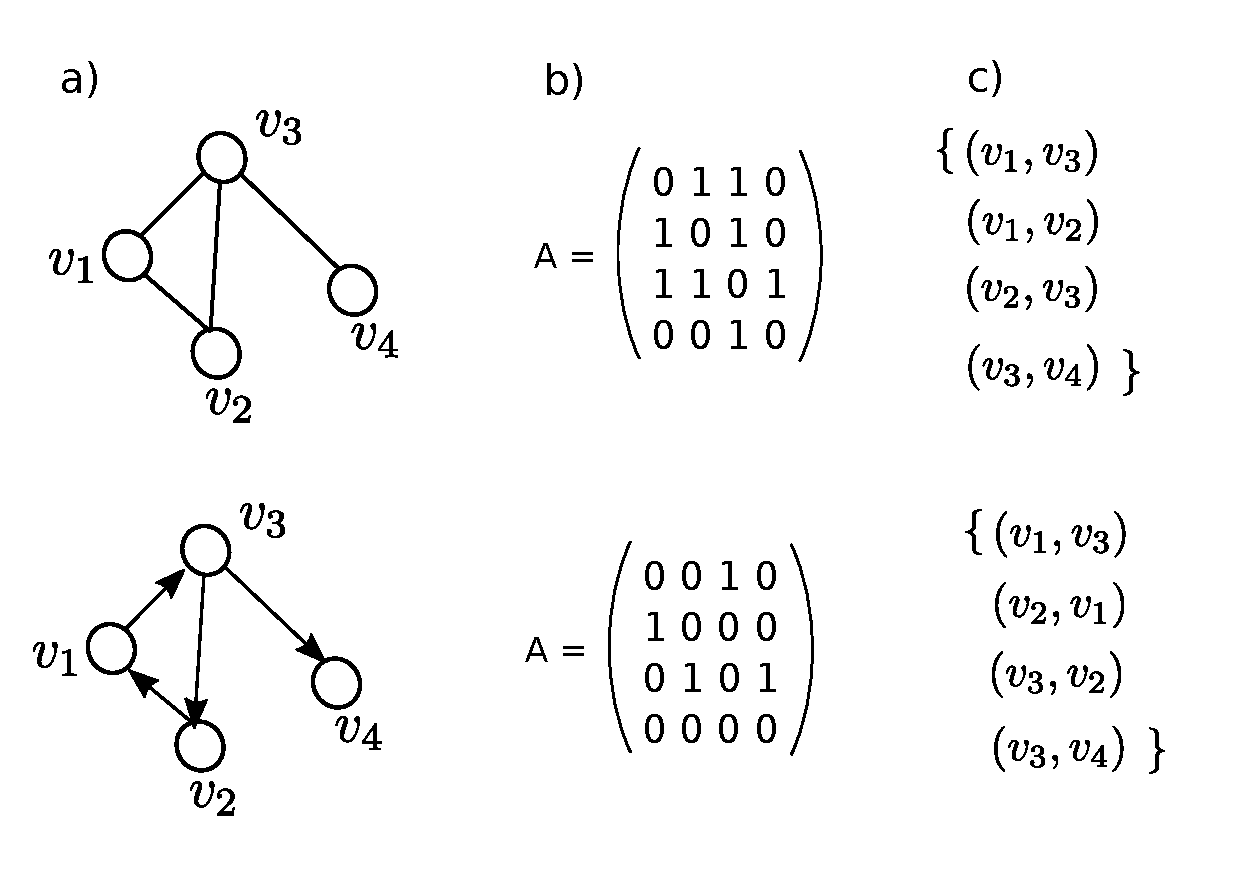
\includegraphics[width=0.7\linewidth]{chapter1/directed_graph.pdf} 
	\caption[Graph, matrix and edge list representations.]{a) Graph representation of undirected (top panel) and directed (bottom panel) network. The same networks are represented with adjacency matrices in column b) and edge list representation in column c).}
	\label{fig:graph_dir}
\end{figure}

The number of edges and nodes are dependent variables. Considering that each node can make $N-1$ connections, the maximum number of the edges in the network is $L_{max}=N(N-1)/2$, as each edge is counted twice. For a directed network, it is possible to draw $L_{max}=N(N-1)$ edges \cite{caldarelli2007scalefree}. When it comes to large networks, they are sparse, meaning that the number of links is $L<<L_{max}$. Consequently, the adjacency matrix is also a sparse structure (has many zeros) that takes a large portion of computer memory \cite{barabasi2016network}. 
It is common to represent the graph as an edge list. In this case, illustrated in Figure \ref{fig:graph_dir}, column c), a graph is described with the list of links that are in the graph, $G = \{ \{v_i,v_j\}\}$. Still, with this representation, we cannot distinguish between directed and undirected graph structures, so the computational algorithm should specify if the edges are symmetric or not.  


\begin{figure}[h]
	\centering
	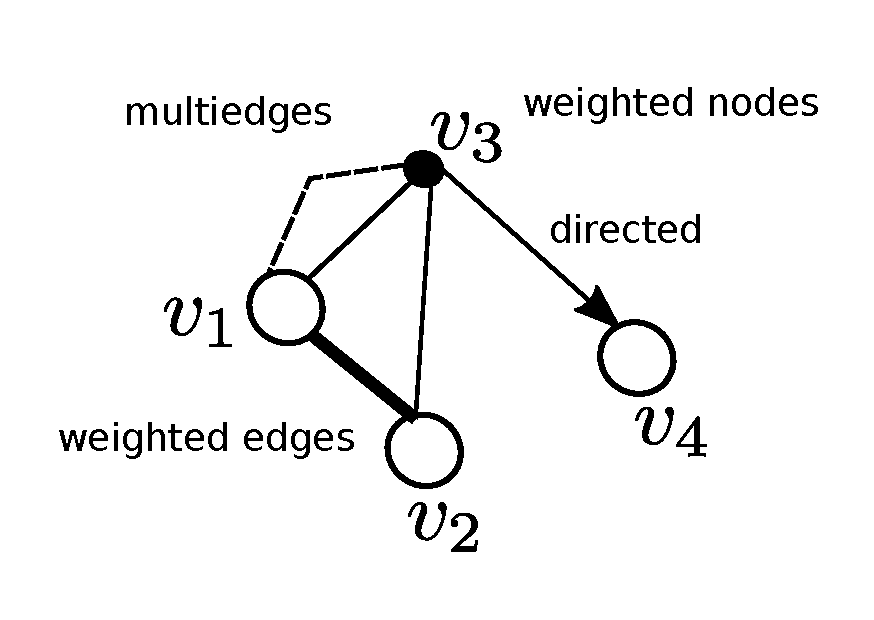
\includegraphics[width=0.4\linewidth]{chapter1/multi_graph.pdf} 
	\caption[Different network representations.]{The complex networks may represent different system characteristics. The edges can be directed, weighted or multiply. Also, nodes can be assigned with different weights or any relevant feature.}
	\label{fig:multigraph}
\end{figure}

Sometimes is essential to include the specific properties of the system in the network representation. For example, to emphasise the frequent interactions between nodes, edges can be assigned with different values; such networks are \textbf{weighted}. In collaboration network authors who colaborate more often have stronger interaction. They can be described with an adjacency matrix, whose elements can take any real number $A_{ij}=w_{ij}$ and $w_{ij}>0$. In general, edges may be associated with any categorical variable. Similarly, properties can be added to nodes or the whole network structure. Edges could be characterised by the time when the interaction between nodes happens, which includes the \textbf{temporal} component in the network representation, as in phone calls networks. Finally, if two nodes interact differently, the \textbf{multigraph} is an appropriate configuration where multiple edges are allowed.The transportation network, consisting of rods and railways could be seen as multigraph. Figure \ref{fig:multigraph} presents the graphical representation of discussed network representations.

A \textbf{bipartite network} consists of two types of nodes. The nodes in the same partition are not connected, while links exist only between partitions. For many real systems, a bipartite graph is a natural representation\cite{barabasi2016network, latora2017complex}. For example, the bipartite network of people and groups has two distinct node partitions, while links indicate the memberships. Another example is a system of customers and products. The user and item link is created when the user buys an item. The bipartite networks find their application in the algorithms for recommended systems, whose goal is to suggest items that may interest the user. Actually, to find the most probable missing links in the network. 

In a bipartite network, nodes in one partition are not connected. Still, we can analyse a single node type if we project the bipartite network on one partition. The primary assumption is that two nodes in one partition could be connected if they point to the same node in another partition. Consider the network of movies and actors. The one-mode projection of movies is an undirected network whose links indicate that two movies share the same actors. On the other hand, another projection is a network of actors. The links exist if two actors appear in the same movie \cite{newman2010, barabasi2016network}.

\begin{figure}[h]
	\centering
	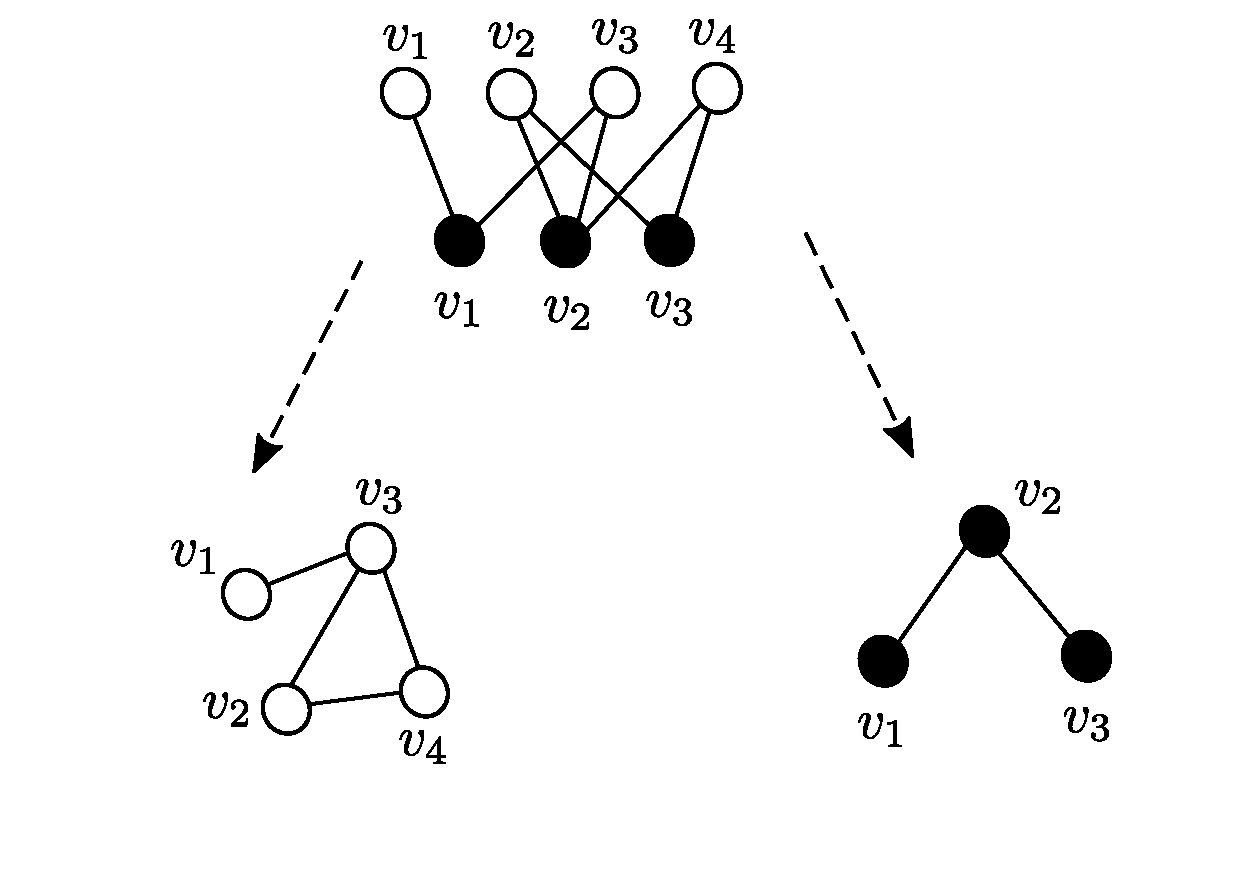
\includegraphics[width=0.7\linewidth]{chapter1/bipartite_graph.pdf} 
	\caption[Bipartite network.]{Bipartite network and two partition projections.}
	\label{fig:gt2}
\end{figure}

We should be aware that important information is lost when creating a one-mode projection. First, having weighted edges in the network of actors is necessary to know how many movies two actors appear. From the one-mode projection, we can not reconstruct the original network. Moreover, two different bipartite networks may have the same projected networks. The important consequence of the network projection is the creation of cliques, i.e. subgraphs where all nodes are connected. \\
In general, it is possible to define the k-bipartite network. The same rules apply as before. There are $k$ distinct node partitions, while the edges exist only between different types of nodes.

\textbf{Temporal networks.}
Studying real systems as static networks can give us a lot of insight into the system's properties. Still, real systems are not static; they evolve not only in the number of elements but also in the number of interactions between them. Some interactions in the system may repeat in different intervals and could be described with complex activity patterns. Including time dimension in the network, representation allows us to study the properties of the system closely. The temporal information may matter a lot \cite{holme2012}. For example, if the interaction between nodes $(v_1, v_2)$ happened before in time than  $(v_2, v_3)$, then nodes $v_1, v_3$ would not be connected, as is the case in the static network. 

The temporal network is a collection of timestamped edges. Each edge is defined as $(v_i, v_j, t, \Delta t)$, where $v_i$ and $v_j$, are nodes $t$ is time when interaction happen, and $\Delta t$ is event duration \cite{guide_temporal}. The duration of the events may vary, as in the phone-call network. Also, for many systems, the time resolution of the event duration is too small. For example, this parameter may be neglected when people interact on social platforms or email each other because the event time is too short; it scales in seconds.

\begin{figure}[h]
	\centering
	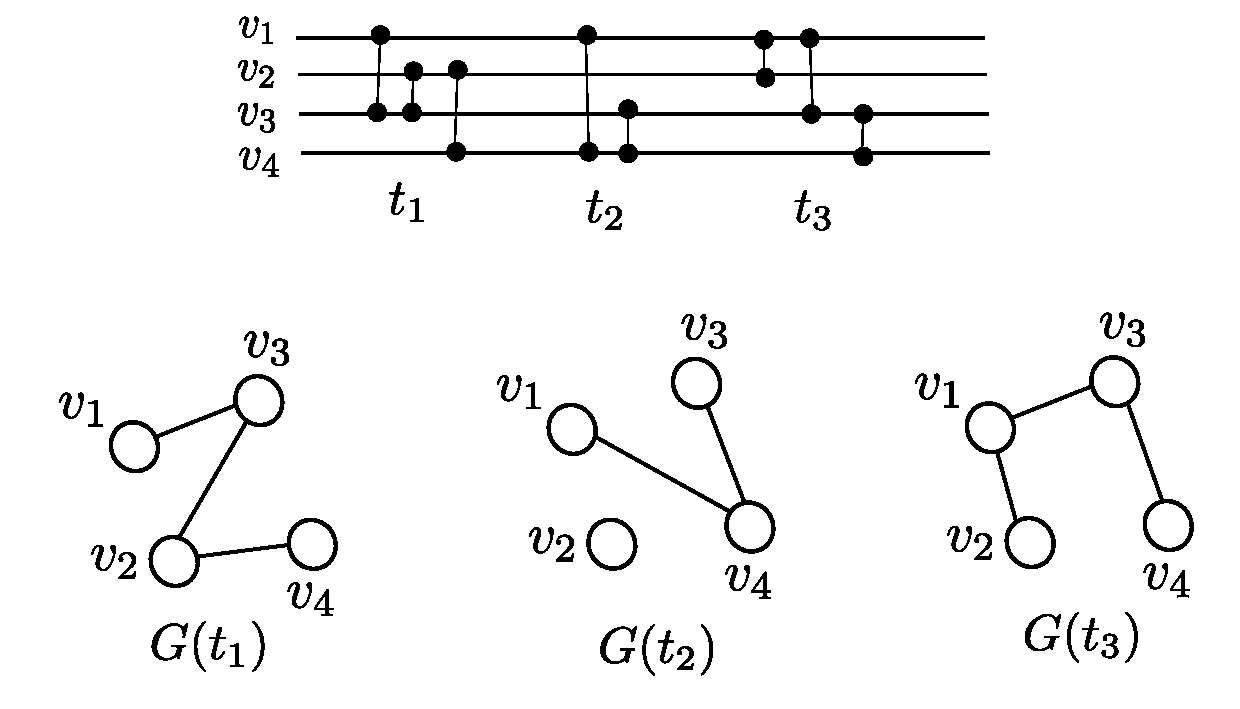
\includegraphics[width=0.7\linewidth]{chapter1/temporal_network.pdf} 
	\caption[Temporal network.]{Temporal network. }
	\label{fig:gt3}
\end{figure}

The temporal network can be represented as a sequence of static networks that evolve in time, $G = \{ G(t_1), G(t_2), ..., G(t_{max})\}$. At each time step, we can create the network and analyse the macroscopic properties of the given network snapshot. With this, we can end up with graph snapshots with many disconnected components or empty graphs for some points \cite{holme2015modern}. Sometimes, a much better approach is to aggregate the links over time windows. Here, we need to specify the time window length $w$. Interactions in the time interval $0\leq t<w$ enter the first snapshot. The following snapshot takes edges $w \leq t <2w$, and so on. The time windows are not overlapping, but generally, it is possible to slide the time window for different periods $ 1 \leq \delta t \geq w$. The downside of this method is that we can not recover original data points. The larger the time window is, the more information is lost. If the time window is set to $w=t_{max}$, there is only one snapshot, and the temporal data are no more available \cite{krings2012effects, arnold2021moving}. 

\textbf{Multilayer networks} were introduced for studying systems in which different types of interaction exist. This formalism allows one to investigate diverse network systems and to combine different types of data into one model \cite{porter2018multilayer}. In a multilayer or multiplex network, all nodes are present in each layer, but their interactions among layers differ. Two nodes may be connected in one layer but not in the other. Different online social systems may be an example of a multiplex network when users are connected on one platform but not on the other \cite{aleta2019multilayer}. Or the airline transportation network, where each layer represents the flights of different airline companies \cite{kivelamultilayer}.  


\section{In this thesis}
%%TODO Ovde mi samo nedostaje jedan paragraf koji kaze koje probleme proucavamo, na kojim sistemima i kako se oni povezuju sa temom.

This thesis uses statistical physics and complex network approaches to model and empirically analyse online social systems. These systems consist of many users interacting online and could be represented by complex networks.  The main focus of the thesis is to explore the evolution of these complex networks and understand how different dynamical processes shape their structure. We study the growth of various online social networks using data from platforms Meetup, Reddit and StackExchange and try to address important structural changes in the systems, what processes lead to the creation of groups and what is important for emergence of the sustainable communities.

In chapter \ref{Ch:Method}, we provide the methodology employed for this research. We describe the fundamental measures of complex networks and introduce basic complex network models. We review the most common probability distributions characterising complex systems' properties and outline distribution fitting methods. Finally, we introduce the multifractality of the time series and dynamical reputation model. 

Chapter \ref{Ch:signals} addresses the difference between network models where the growth in a number of nodes is constant and when it follows a non-trivial growth signal. This research aims to quantify how growth signals influence the structure of complex networks. Using the adapted ageing model \cite{hajra2004}, we use computer simulations to generate different kinds of complex networks. For more realistic real-world network simulations, growing signals are time series of new users from online social platforms, MySpace and Tech group from Meetup. They are described with trends, cycles and long-range correlations. Often time series have multi-fractal properties. The results of this study are published in \cite{vranic2021growth}, and they show the importance of growth signals in shaping the network structure because the scale-free networks, which represent real systems, are mainly altered. 

As research on social groups mainly focuses on a single group, there are remaining questions about the characteristics of the entire system. For example, the Tech group is only one of the groups around which Meetup users organise; many other groups are created worldwide, so the system constantly grows. In chapter \ref{Ch:Groups}, we will examine how groups on online social platforms grow. The results are summarised in the paper  \cite{vranic2022universal}. This research is based on Reddit and Meetup data. From Meetup, we created two data sets, one with groups created in London and the other with groups created in New York, while for Reddit, we selected groups built before 2012. We are interested in explaining scaling behaviour in group size and growth rate distributions and identifying the growth mechanisms present in the system. Using a bipartite complex network model, we can reproduce the universality found in the system.

Even though across complex systems, we find the emergence of universal behaviour, for example, the scaling of the degree distribution of two groups is similar, different factors might influence its success. It is well known that many online groups may suddenly fall apart. These questions are the subject of the chapter \ref{Ch:Trust}, which main results are published in the paper \cite{vranic2022sustainability}. Here, we study the question-answer platform Stack Exchange; it has more than 200 different topic-specified sites where people help each other answer questions. What is interesting about this system is that some sites were closed because they did not produce enough activity. For that reason, we selected the sites with the same topic that failed but later, when someone proposed the site again, it stayed active. We analyse the evolution of user interaction networks; here, we use the temporal network approach and compare active and closed sites. We find that it is essential how the network users are distributed into a core-periphery structure \cite{gallagher2020clarified}. The core must select firmly connected users, but their interaction with the periphery has to be high. In other words, we need a trustworthy core to hold the community. Introducing the Dynamical Reputation Model (DIBRM) \cite{melnikov2018toward}, based on user interaction sequences, we quantify how much users can be trusted and whether the community has a strong core. In the appendix \ref{App:SE}, we briefly describe the Stack Exchange sites. In appendix \ref{App:parameters} and \ref{App:sliding} discuss how we choose parameters for the DIBRM model, while in appendix \ref{App:robust} we discuss the stability of inferred core-periphery structures. 

Finally, in chapter \ref{Ch:Conclussion}, we draw the main findings of this thesis. 

\selectlanguage{english}















%\chapter{Methodology} % Main chapter title
\label{Ch:Method}

\section{The measures of complex network structure}
%%TODO 2.1 The measures of the complex networks structure

The complex system can be represented by a complex network $G=(V, E)$, where the elements of a system (atoms, proteins, people) map to a set of $N$ nodes $V=\{1, 2, ..., N\}$. The interactions between elements map to $L$ links between nodes, $E = \{ e_1, e_2... e_L\}$. There are a lot of measures to quantify the structure of the network. This section describes some of the important measures and their definitions on the undirected and unweighted networks, where the \textbf{adjacency matrix} ${A} = N \times N$ has value $1$ if there is a connection between two nodes; otherwise, it is $0$ \cite{boccaletti2006complex}; as this network representation is mostly used through the thesis. We list degree distribution, correlations, and shortest path measures. We also discuss different structures found in the network, such as core-periphery or community structures.   

%The \textbf{adjacency matrix} ${A} = N \times N$ has value $1$ if there is a connection between two nodes; otherwise, it is $0$ \cite{boccaletti2006complex}.
%%TODO Ovakvom recenicnom kao da kazemo da samo imamo binarne mreze. Mozda bi bilo bolje da pre toga kazemo da cemo mi koristiti mahom binarne mreze. I onda ova recenica.
%There are a lot of measures to quantify the structure of the network. This section lists the most important measures, such as degree distribution, correlations, and shortest path measures. We also discuss different structures found in the network, such as core-periphery or community structures.  

\subsection{Degree distribution}

The simplest network measure is \textbf{node degree}, $k$. The degree of node $i$ is %gives %TODO is or equal 
the number of nodes adjacent %attached %TODO adjacent
 to node $i$, $k_i = \sum_j A_{ij}$. The network density is the average degree divided by $N-1$, where $N$ is the number of nodes. %It is a relative fraction of nodes in the network.%TODO sta je ovo
 
In the case of regular networks, such as grids, each node has an equal degree, meaning that nodes in the network have similar roles. In the general case, the networks have a more complex structure. If the degree sequence is skewed, we can identify nodes with high-degree (hubs). Removing hubs may partition a connected network into several components \cite{albert2000error}. %%TODO nedostaje citat
 
The degree distribution is the probability, $P(k)$, that a randomly chosen node has degree $k$. To estimate the degree distribution, we can consider the fraction of $k$ degree nodes $N_k$, $p(k) = N_k/N$. Similarly, we can order nodes according to their degree and plot the node degree.

%To estimate %calculate %TODO estimate. 
%%TODO Bolje bi bilo da uvedes pro sta je P(k) pa onda kako je procenjujemo. 
%the degree distribution, we can consider the fraction of $k$ degree nodes $N_k$, $p(k) = N_k/N$. It is the probability, $P(k)$, that a randomly chosen node has degree $k$. Similarly, we can order nodes according to their degree and plot the node degree.

%If the graph nodes are statistically independent, the degree distribution completely determines the properties of a network \cite{dorogovtsev2002evolution}.%TODO ovo je nejasna recenica
Here we summarize the forms of degree distributions that are mostly found in the complex network theory:
\begin{itemize}
	\item The Poisson distribution. The degree distribution in a random network, where all nodes have the same connecting probability, follows Poisson distribution $P(k)= \frac{(Np)^ke^{-Np}}{k!}$, where $k$ is the mean degree distribution. 
	
	\item Exponential distribution. $P(k) = e^{-k/ \- k}$. It is the degree distribution of the growing random graph. Even for infinite networks, all moments of distributions are finite and have a natural scale of the order of average degree.
	
	\item In many real networks, degree distribution follows a power law. $P(k) = k ^ {-\gamma} $, where $\gamma$ is exponent of the distribution. No natural scale exists in this distribution, so they are called scale-free networks. In infinite networks, all higher moments diverge. If the average degree of scale-free networks is finite, then the $\gamma$ exponent should be $\gamma>2$. Therefore, real networks have a scale-free structure with the emergence of the hubs \cite{newman2010}. 
	%In finite-size networks, fat-tailed degree distributions have natural cutoffs. 
\end{itemize}

When plotting the degree distribution, it is common to use scaling of the axis. As many nodes have a low degree, like for power-law or exponential distribution, it is more useful to use a logarithmic scale. Now it is easier to notice that data points follow a straight line, meaning that degree distribution is some exponential function. 

\subsection{Degree-degree correlations} %%TODO Degree-degree correlations.

Correlation is defined through a correlation coefficient r. If x and y are two stochastic variables, for which we have a series of observation pairs $(x_1, y_1), (x_2, y_2), ...,(x_n, y_n)$. The correlation coefficient $r(x, y)$ between $x$ and $y$ is defined as \cite{van2010graph}:

\begin{equation}
r(x, y) = \frac{\frac{1}{n}\sum_{i=1}^{n}((x_i - \bar{x} ) (y_i - \bar{y}) )}{\sqrt{\frac{1}{n}\sum_{i=1}^{n}(x_i - \bar{x})^2} \sqrt{\frac{1}{n}\sum_{i=1}^{n}(y_i - \bar{y})^2} }
\end{equation}

where $\bar{x} = \frac{1}{n}\sum_{i=1}^{n}x_i$, is the average over variable $x$.

Using the correlation coefficient definition, we can define correlations for vertex degrees. For simple graph G with vertex set $V(G) = \{v_1, ..v_n\}$, $\boldsymbol{A}[i,j] = 1$ if there is a link between nodes $v_i$ and $v_j$. If G is a simple graph with adjacency matrix $\boldsymbol{A}$ and degree sequence $\boldsymbol{d} = [d_1, ..., d_n]$

\begin{equation}
r_{deg}(G) = \frac{\sum_{i=1}^{n}\sum_{i=1+1}^{n}((d_i - \bar{d}) (d_i - \bar{d}) \boldsymbol{A}[i,j] )}{\sum_{i=1}^{n}(d_i - \bar{d})^2}
\end{equation}

An adjacency matrix allows us to calculate the correlations between neighbouring nodes. If two nodes are not connected $A[i,j]=0$, the degree of correlation between them does not contribute to the $r$.

The \textbf{degree-degree correlations} in the network are measured by \textbf{assortativity index}. %%TODO assortativity index ne assortatiity. I nije jedino meren tako,
If correlations are positive, networks are assortative; there is a tendency for connections to existing between similar degree nodes. The negative correlations indicate that large-degree nodes prefer to connect nodes with a small degree, disassortative networks. The average first neighbor degree $k_{nn}$ can be calculated as $k_{nn} = \sum_{k^{'}}k^{'}P(k^{'}|{k})$. The $P$ is the conditional probability that an edge of degree $k$ points to a node with degree $k$. The norm is $\sum_{k^{'}}P(k^{'}|k)=1$, and detailed balance conditions \cite{boccaletti2006complex},  $kP(k^{'}|k)P(k) = k^{'}P(k|k^{'})P(k^{'})$ \cite{boccaletti2006complex}. If the node degrees are uncorrelated, $k_{nn}$ does not depend on the degree; otherwise, increasing/decreasing function indicates positive/negative correlations in the network \cite{park2003}.

The Newman defined the assortativity \cite{newman2002assortative} index $r$ in slightly different way:

\begin{equation}
r = \sum_{kl}kl(e_{kl} - q_lq_k) / \sigma_q^2 ,
\end{equation}

where $e_{kl}$ is the probability that a randomly selected link connects nodes with degrees $k$ and $l$, $q_k$ is a probability that a randomly chosen node is connected to node $k$ and equals $q_k = kp_k / \langle k \rangle$, while $\sigma_q$ is a variance of the distribution $q_k$. 

\subsection{Clustering coefficient}

The \textbf{clustering coefficient} is a measure describing the neighbourhood's structure. In networks, exist a tendency to form triangles or clusters \cite{barabasi2016network}. It is common in friendship networks where two friends of one person have a high probability of being friends \cite{mata2020complex}. %. %TODO citat nedostaje
The clustering can be measured by computing the number of links between neighbours of one node \cite{watts1998collective},
\begin{equation}
c_i=2e_i/(k_i(k_i-1))
\end{equation}

We can calculate the mean clustering coefficient by averaging it overall network nodes. It ranges from  $\langle c \rangle = 0$ where connections between neighbouring nodes do not exist; the network has a tree structure. On the other hand, $\langle c \rangle = 1$ indicates a fully connected network. 

Newman proposed the alternative definition for the clustering coefficient based on the number of triples and triangles in a graph \cite{newman2009random}. A triangle at node $v$ is a complete subgraph with three nodes, including $v$. A triple on the node v is a subgraph of exactly three nodes and two edges, where v is incident with two edges. The network transitivity is the ratio of the number of triangles in the network over the number of triples. The network transitivity is seen as global clustering, as it considers the whole network.  

\subsection{Paths} %Network paths} %TODO moze samo paths
In the network structure, the interacting nodes are directly connected with the edge. In this representation, the distance between them is $d_{v_i, v_j} =1 $. Distance defined like this does not have any physical meaning, and its purpose is to describe how the position of nodes in the network structure influences the other distant nodes. 

The \textbf{path} between two nodes \cite{van2010graph}, $v_i$ and $v_j$ is a sequence of edges $\{(v_1, v_2),  (v_2, v_3), ...(v_k, v_{k+1})\\,... (v_{n-1}, v_n)\}$, where $v_1=v_i$, $v_n=v_j$. In the path, the nodes are distinct. Otherwise, the sequence is called a \textbf{walk}, where each node can be visited many times. Also, it is possible to define a \textbf{cycle}, a path that starts and ends on the same node while other nodes in the cycle are distinct. The length of the path, walk or cycle is the number of links in the sequence. We can easily calculate the number of walks between two nodes using the adjacency matrix. The $A^2$ gives us walks of length $2$, the $A^3$, the number of walks of length 3, and so on. 

The network is connected if it can define the path between every two nodes. When it is not the case, the network is disconnected into two or more connected components. Note that the component can be an isolated node. Also, in directed networks may happen that node $v_i$ is reachable from node $v_j$, but if we start from $v_j$, we can not find the path to the $v_i$. Such a graph is connected but is called a weakly connected component \cite{jackson2010social}.

We can find different paths between two nodes in the network, but the most important one is the \textbf{shortest path} \cite{van2010graph, jackson2010social}. The distance between two nodes $d(v_i, v_j)$ is defined as the shortest path length between two nodes. 
In the case of weighted networks, it is the path with minimal weight, and the length of such a path does not have to be minimal. Distances on the network can give us insight into how similar networks are and indicate the node's relative importance in the network. 

%The node's eccentricity shows how far the farthest vertex is positioned in the network. 
The \textbf{radius} is the minimum overall eccentricity value. In contrast, the \textbf{diameter} defines the largest distance between nodes in the network \cite{van2010graph}. These definitions apply to directed and undirected graphs. 

If G is a connected graph with vertex set V and $\bar{d}(u)$ is the average length of the shortest paths from node u to any other node v in network G \cite{van2010graph}.

\begin{equation}
\bar{d}(u) = \frac{1}{|V|-1} \sum_{v\in V, v \notin u} d(u,v)  
\end{equation}

From there, the \textbf{average path length} is the mean value over $\bar{d}(u)$.

\begin{equation}
\bar{d}(G) = \frac{1}{|V|}\sum_{u \in V} \bar{d}(u)
\end{equation}

while the \textbf{characteristic path} length of G is median over all $\bar{d}(u)$.


\subsection{D-measure}

For each node $i$, we can define the distribution of the shortest paths between node $i$ and all other nodes in the network, $P_{i}=\{p_{i}(j)\}$, where $p_{i}(j)$ is percent of nodes at a distance $j$ from node $i$. The connectivity patterns can efficiently describe the difference between the two networks.    
To specify how much $G$ and $G^{'}$ are similar we use D-measure \cite{tiago2}
\begin{equation}
D(G, G^{'}) = \omega \left| \sqrt{\frac{J(P_1,..P_N)}{log(d)}}-\sqrt{\frac{J(P_1^{'},..P_N^{'})}{log(d^{'})}} \right| + (1-\omega) \sqrt{\frac{J(\mu_{G},\mu_{G^{'}})}{log2}}
\label{eq:dmeasure}
\end{equation}

D-measure calculates Jensen-Shannon divergence between $N$ shortest path distributions,

\begin{equation}
J(P_1,.., P_N)) = \sum_{i,j}p_i(j)log(\frac{p_i(j)}{\mu_j})
\end{equation}

where  $\mu_j = (\sum_{i=1}^N p_i(j))/N$ is mean shortest path distribution.

The first term in equation \ref{eq:dmeasure} compares local differences between two networks, and Jensen-Shannon divergence between $N$ shortest path distributions $J(P_{1},..., P_{N})$ is normed with network diameter $d(G)$. The second part determines global differences, computing  ${J(\mu_{G},\mu_{G^{'}})}$ between mean shortest path distributions. The D-measure ranges from $0$ to $1$. The lower D-measure is, the more similar networks are, and structures are isomorphic for D-measure $D = 0$.

\newpage

\section{Community structure}

Nodes can be organized into groups called communities. In social networks, communities indicate that people share some common interests, or in biological networks, we can find that genes or neurons with similar functions are grouped. Identifying these hidden blocks can lead to interesting insights into the network. However, the community detection problem does not give a precise characterization of what a community is. A standard definition of a community is densely connected subgraph \cite{fortunato2010community, martin}, meaning that nodes in one community tend to associate, creating the assortative connectivity pattern. On the contrary, nodes could be organized in disassortative communities, where connections between groups are denser. 

The network with $k$ communities could be represented using $k \times k$ matrix $p$. The diagonal elements of $p$ indicate the density inside communities, while off-diagonal elements show the density between groups. Figure \ref{fig:SBM} \cite{fortunato2016community} shows the matrix and networks for two communities. In the first example, (\ref{fig:SBM} a), the diagonal elements have a higher probability, as in the classic definition of assortative community structure. In disassortative structure (\ref{fig:SBM} b), more connections exist between two partitions than inside them, i.e. off-diagonal elements have higher probabilities. Bipartite networks can be represented as a disassortative network with two groups. The links exist only between communities. Figure (\ref{fig:SBM} c) shows the core-periphery network. This network structure is composed of a core where nodes are well connected with itself and with the periphery. The connectivity inside the periphery is sparse. Finally, if there is no difference between connectivity inside and between groups, the concept of communities is lost. We can treat the whole network as a single community, where each node has the same connectivity probability, i.e. as Erdos Renyi random graph. 

\begin{figure}[h]
	\centering
	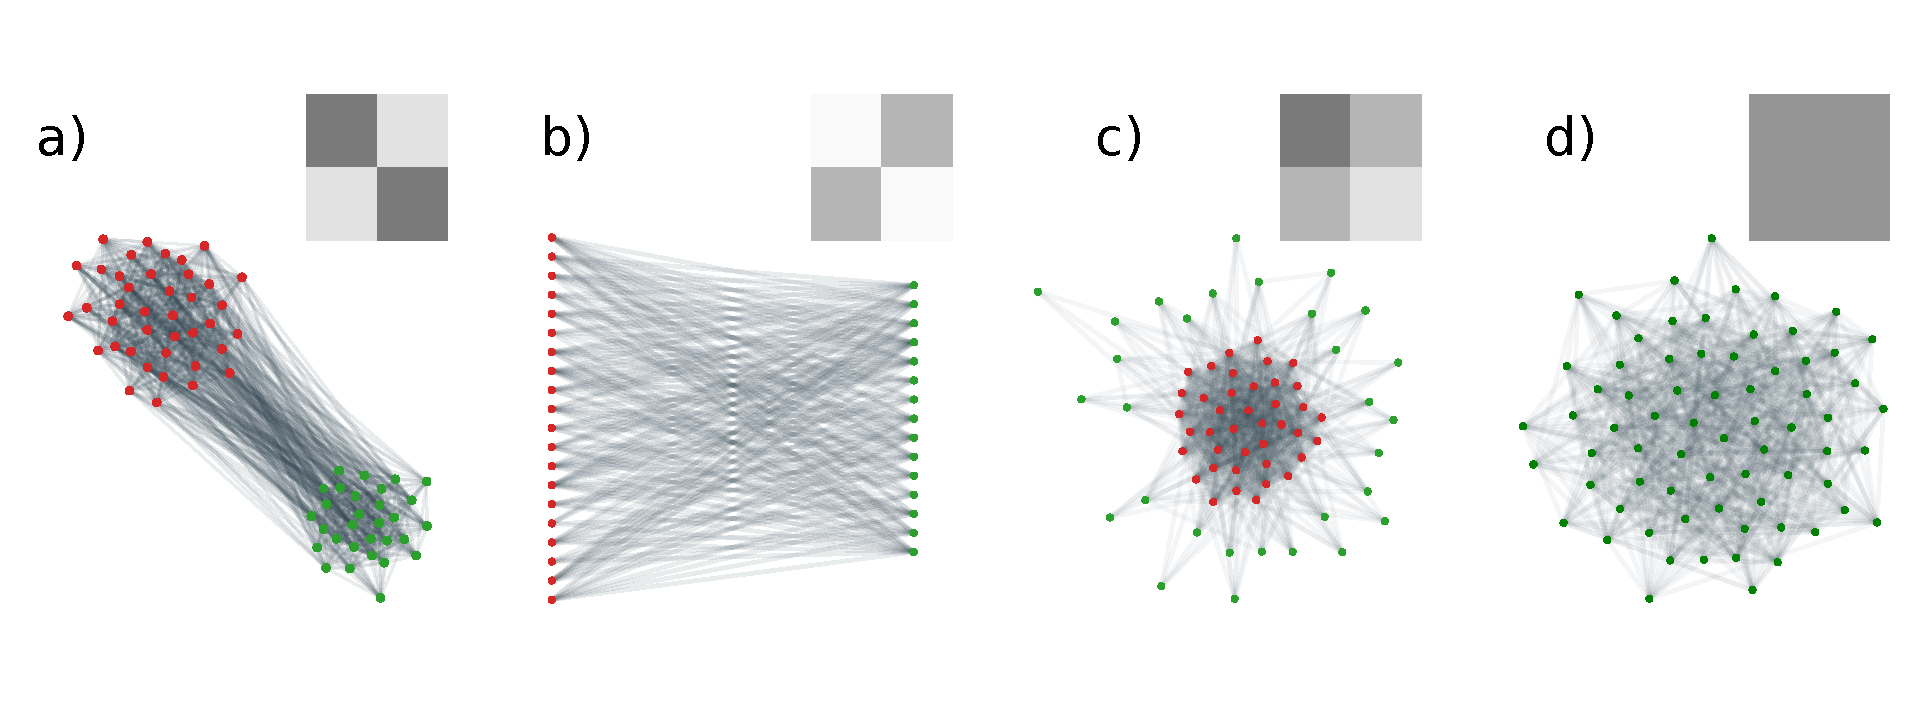
\includegraphics[width=1.\textwidth]{chapter2/SBM_representations_1.pdf}
    %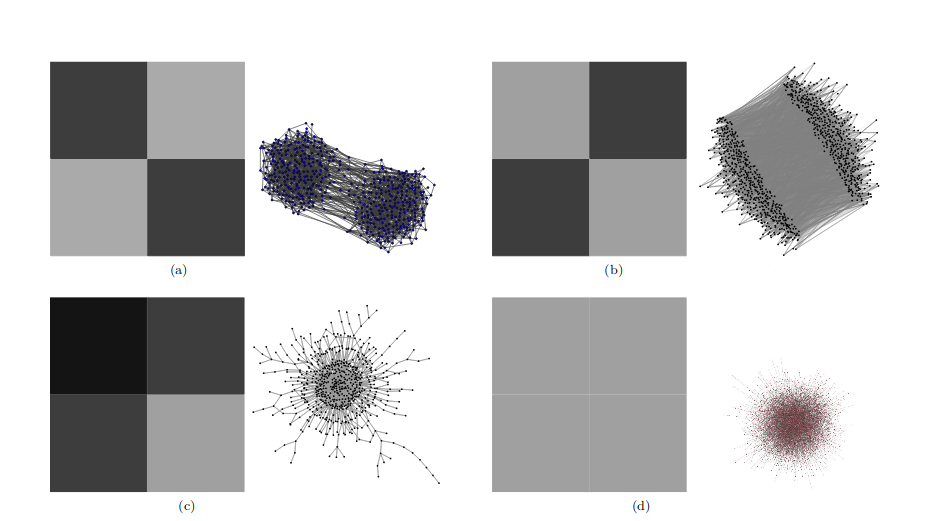
\includegraphics[width=0.8\textwidth]{chapter2/structures.png}
	\caption[Stochastic Block Model]{ Different communities structures  (a) assortative. (b) disassortative. (c) core-periphery. (d) Erdos Renyi random graph.}
	\label{fig:SBM}
	%TODO ima li ova slika u boji? mozda uzeti prava
\end{figure}

Different algorithms are used for detecting the community structure in the underlying network, optimizing different objective functions of the network partition. Still, if the ground-truth communities are unknown, there are no guarantees that we will infer the actual number of communities and entirely correct node assignments \cite{peel2017ground}. Even though community detection algorithms are widely used in complex network analysis as they can give us a better understanding of network structure \cite{peel2017ground, cherifi2019community}.  %%TODO citat
In this section are explained two community detection models, the first one based on optimizing the modularity function \cite{fortunato2010community, guimera2004modularity}, and the other based on the statistical inference of the Stochastic Block Model (SBM) where is optimized the likelihood function \cite{fortunato2010community, lee2019review, peixoto2019bayesian}. %%TODO citat

\subsection{Community detection based on modularity function optimization} 

Comparing the link density of the community with the link density obtained for the same group of nodes randomly connected, we could conclude if the community corresponds to the dense subgraph or if the structure is created entirely random. The \textbf{modularity} \cite{newman2004finding, guimera2004modularity, good2010performance} is a function that measures the randomness of each partition. %%TODO definisati sta je partition
Partition is division of the network into $n_c$ groups, where each node belongs to only one group \cite{barabasi2014network}. 
%While in graph partitioning the number and the size of communities is predefined, in community detection both parameters are unknown. We call a partition a division of a network into an arbitrary number of groups, such that each node belongs to one and only one group. The number of pos 10 0 sible partitions follows
%We can compare the communities with modularity and decide which one is better. 
For the network with $N$ nodes and $L$ links partitioned into $n_c$ communities where each community has $N_c$ nodes and $L_c$ links. If the number of connections is larger than the expected number of links between $N_c$ nodes given in the expected node sequence, these nodes may form the community. We calculate the difference between real network connectivity $A_{ij}$ and the expected number of links between nodes if the network is randomly connected, $p_{ij}$. The $p_{ij}$ can be obtained by randomizing the original network but keeping the expected degree of each node unchanged, so $p_{ij}= \frac{k_ik_j}{2L}$.

\begin{equation}
M_c = \frac{1}{2L}\sum(A_{ij}-p_{ij})
\end{equation}

If modularity is positive, the selected nodes may be a community, as their connectivity is far from random. If $M_c$ is zero, then the connectivity between nodes is arbitrary, and if $M_c$ is negative, the nodes do not form the community.  The same idea can be generalized to the whole network: The modularity of the network partitioned into $n_c$ communities is then defined as:
\begin{equation}
M=\sum_{c=1}^{n} [\frac{L_c}{L} - (\frac{k_c}{2L})^2]
\end{equation}

The higher modularity indicates that nodes are partitioned in better communities. When we put all nodes into only one community $M=0$, otherwise, if each node is the community itself $L_c=0$ and the sum is negative. The Newman showed that modularity function  \cite{newman2004analysis} applies for weighted networks.

Maximum network modularity indicates the best partions. As too many possible partitions exist, we need an algorithmic approach to identify the best separation. The first algorithm proposed for modularity optimization was \textbf{greedy algorithm}. First, it assigns each node to a community and starts with N communities. Then, we should merge each pair of communities and calculate the modularity difference $\Delta M$. We can join those two communities by identifying the pair for which the difference is the largest. It is repeated until all nodes merge into a single community. The best partition is one with the largest $M$.

\textbf{Louvain algorithm} \cite{blondel2008fast} is an optimization algorithm with better scalability than the greedy algorithm so it can operate on very large networks. Initially, each node is assigned to a different community, and similar to before, we calculate the difference in the modularity moving nodes to one of their neighbouring community. Then we move node $i$ to the community such that modularity becomes larger. It is applied to all nodes until no further improvement can be made. In the second step, we create a weighted network whose nodes are communities identified during the first step. The weight of the links between communities is the sum of the weights between nodes. The number of links inside the community is given as a weighted self-loop. Then, the first and second steps are repeated until there is no more change in the modularity. The obtained number of clusters when algorithm stops is optimal number of communities. 

The community detection algorithms tend to merge small communities, which should be independent \cite{fortunato2007resolution}. This consequence is easily seen in graph consisting of N connected cliques, where higher modularity is if two adjacent cliques are merged into communities, instead having each clique as single community. This lead to the modification of the modularity function as $M= \frac{1}{2L}\sum_{i,j}[A_{i,j} - \gamma \frac{k_ik_j}{2L}]$, where $\gamma$ is resolution parameter \cite{reichardt2006statistical}, which controls the size of communities to be detected. With $\gamma<1$, it would be possible to detect small communities undetected with original model. 

%%TODO Posto je sekcija o Louain algoritmu, treba dodati jos par paragrafa o njemu. Konkretno njegove karakteristike (otezinjeni, usmereni grafovi...), zatim reyolucija, i najbitnije kako odredjuje optimalan broj zajednica. Pogledaj neki od Santoih poslednjih radoa na temu zajednica.



\subsection{Stochastic block model}

Another approach for studying the community structure of complex networks, the Stochastic Block Model (SBM), assumes that nodes are clustered in the groups, and the relations between nodes depend on the probabilities for group memberships \cite{lee2019review}. In one group, nodes have similar connectivity patterns. To describe the network $G(N, L)$ with the SBM model, we need to define the following:

\begin{itemize}
	\item k: number of groups
	\item group assignment vector, g: $g_i \in\{1,2..k\}$, gives the group index of node $i$.
	\item SBM matrix, $p_{k \times k}$, whose elements $p_{rs}$ are the probabilities that edges between groups $r$ and $s$ exist. Note that nodes within one group have the same connection probabilities. 
\end{itemize}

The number of possible nodes between two groups $r$ and $s$:
\begin{equation}
n_{rs} = \begin{cases}
n_r(n_{r}+1)/2 &\text{if  } r=s \\
n_rn_s &\text{if  } r=s\\, 
\end{cases}
\end{equation}
while the number of possible edges depends on the adjacency matrix $A_{ij}$:
\begin{equation}
e_{rs}=\frac{1}{1+\delta_{rs}}\sum_{i \in r, j\in s} A_{ij}
\end{equation}



The benefit of this model is that we can \textbf{generate} many networks with similar network structure \cite{rosvall2019different}. When model parameters are initialized, the network can be easily generated. For each pair of nodes $i$ and $j$ in network $G$, we draw a link if random number $r_{ij}<p_{r, s}$. 

The likelihood of generating network $G$ for given model parameters is:
\begin{equation}
P(G|p, g) = \prod_{i,j} Pr(i \rightarrow j| p, g) = \prod_{(i,j)\in E} Pr(i \rightarrow j| p, g)\prod_{(i,j)\notin E} ( 1 - Pr(i \rightarrow j| p, g))
\end{equation}

In the processes where the connection between two nodes is described with Bernoulli distribution, the likelihood takes the form:
\begin{equation}
P(G|p, g) = \prod_{(i,j)\in E} p_{g_ig_j}\prod_{(i,j)\notin E} ( 1 - p_{g_ig_j})
\end{equation}

In the likelihood equation, we iterate over all pairs of nodes, separating the product over edges present in the network and edges that are not present.  
As all nodes are considered independent, we can switch the product over nodes with the product over groups such that
\begin{equation}
P(G|p, g) = \prod_{(r,s)} p_{rs}^{e_{rs}}(1-p_{rs})^{n_{rs}-e_{rs}}
\end{equation}
As it is easier to work with the logarithm of the likelihood function, after taking the logarithm of the likelihood function, we get the following expression:
\begin{equation}
L = log(P(G|g, p)) = \sum_{r,s} e_{r,s} ln\frac{e_{rs}}{n_{rs}} + (n_{rs}-e_{rs})ln(\frac{e_{rs}-e_{rs}}{n_{rs}})
\end{equation}

Instead of generating networks, the opposite task is network \textbf{inference}. For a given network $G$, and specified the number of communities $k$, we can use the SBM model to infer the nodes' assignments into groups, so we need to choose vector $g$ and SBM matrix $p$ such that the likelihood for generating network $G$ is maximized. 

The formulation of the SBM model does not consider how to infer the optimal number of groups. Optimizing the likelihood function for different numbers of groups would increase likelihood while each node is not assigned to a different group. In practice, our found community structures for a fixed number of groups, and then the likelihood function could be penalized by the number of model parameters. One approach is calculating the \textbf{Minimum description length (MDL)} \cite{peixoto2019bayesian}. For the variable that occurs with probability P(x), the necessary amount of information to describe it is $-log_2P(x)$. The numerator of posterior probability could be written as
\begin{equation}
P(G|g)P(g) = P(G|p, g)P(p, g)=2^{-\Sigma}
\end{equation}
where $\Sigma$ is the data's description length (DL). It means that if we find the network partition that maximizes the posterior distribution, we also find the MDL. The MDL consists of two terms: $\Sigma = -log2(p(G|p,g))-log2P(p,g)$. In the first part of the equation, the amount of information necessary to describe the model decrease with the number of groups. The second contribution comes only from the model, and as the model becomes more complex, with a larger number of groups, this part increases. The optimal solution represents the balance between these two terms in the MDL equation.  

This SBM model has many variants motivated by specific properties of real data. For example, for degree heterogeneous networks, there is degree corrected SBM \cite{karrer2011stochastic}. In some social networks, users can belong to more than one group, which can be modelled with mixed membership SBM. Other extensions include application to bipartite, weighted network, and hierarchical model \cite{funke2019}. Many community detection algorithms define the community as an assortative structure. With the SBM model, such limitations do not exist, and it is possible to directly use statistical inference for discovering core-periphery structures or even networks with bipartite structures.  

\subsection{Core-periphery structure}

Core-periphery structure describes a network whose nodes are divided into two communities, densely connected core and less connected periphery \cite{csermely2013structure}. With the average probabilities of edges within each group as $p_{11}$ and $p_{22}$, and between groups $p_{12}$, the core-periphery structure is defined under the condition  $p_{11}> p_{12} > p_{22}$. The simple method for finding core-periphery structures assumes that core nodes have higher degrees in the core than in the periphery. Another simple method is to construct k-cores \cite{malliaros2020core}. K core is a group of nodes connected to at least k other members. K-cores form a nested set and become denser with higher k. The core-periphery structure can be detected by optimizing the measure similar to modularity, as defined by Borgatti and Everett \cite{borgatti2000models}. Their goal is to find the division that minimizes the number of edges in the periphery. So they define the score function as equal to the number of edges in the periphery minus the expected number of such edges placed randomly. $\rho = \frac{1}{2}\sum_{ij}(A_{ij}-p)g_ig_j$.

Another way to detect core-periphery structure is to use the inference method based on fits to a Stochastic Block Model (SBM) \cite{zhang2015identification, karrer2011stochastic}. In this method, we fit the observed network to a block model with two groups, such that edge probabilities have the form $p_{11}> p_{12} > p_{22}$. Vector $\theta_i = r$ indicates that node $i$ is in block $r$, while SBM matrix $\{p\}_{2x2}$, specify the probability $p_{rs}$ that nodes from group $r$ are connected to nodes in group $s$. The SBM model is looking for the most probable model that can reproduce a given network G \cite{gallagher2020clarified}. 
Probability of having model parameters $\theta, p$ given network $G$ is proportional to the likelihood of generating network $G$, prior of SBM matrix $P(p)$ and prior on block assignments $P(\theta)$: $P(\theta, p| G) = P(G | \theta , p) P(p) P(\theta)$, while the likelihood function takes following form: $P(G | \theta , p) = \prod_{i<j} p_{r_is_j}^{A_{ij}}(1-p_{r_is_j})^{1-A_{ij}}$, where $A_{ij}$ is a number of edges between nodes $i$ and $j$. The prior $P(p)$ is modified for core-periphery model such that $P(p)  \sim I_{0<p_{22}<p_{12}<p_{11}<1}$, while prior  $P(\theta) $ consists of three parts: probability of having $2$ blocks; given the number of layers probability $P(n|2)$ of having groups of sizes ${n_1, n_2}$ and the probability $P(\theta|n)$ of having particular assignments of nodes to blocks. 



\section{The probability distributions}
%%TODO mozda zameniti 2.3 i 2.4

The shape of degree distribution is important for getting the first insight into the characteristics of the complex network. When nodes are generated randomly, and any two nodes are linked with the same probability $p$,  we expect the binomial distribution. For larger networks it is Poisson distribution $P(k) = \frac{1}{k!}e^{-\langle k \rangle}\langle k \rangle^{k}$, where $\langle k \rangle = Np$. A different approach is to add one node and connect it randomly to the network at each time step. The obtained network then has the exponential degree distribution $P(k)=e^{-\lambda k}$. These are exponentially bounded distributions, meaning they decay exponentially or faster for the large values \cite{barabasi2016network}. 

On the other hand, heavy-tailed distributions decay slower than exponential, and the events for large values are rare but still possible. For example, in the preferential attachment model, degree distribution emerges to the power law \cite{barabasi2016network}. Also, many empirical data exhibit the heavy-tailed distribution. Even if they look like a power law, after statistical analysis, it may be concluded that the data deviate from the power law and could be equally good or even better fitted with some other distribution. Commonly used alternative distributions are lognormal distribution, stretched-exponential or power-law with an exponential cutoff. 

This section gives an overview of relevant distributions and methods for fitting data and testing the quality of the performed fit. Figure \ref{fig:distributions} shows how different distributions look on linear (first column) and log-log scale (second column).

%TODO Mozes da se ovde fokusiras na realne mreze vise neko na modelirane. Jer na kraju sve je krenulo od njih.

\begin{figure}[!h]
	\centering
	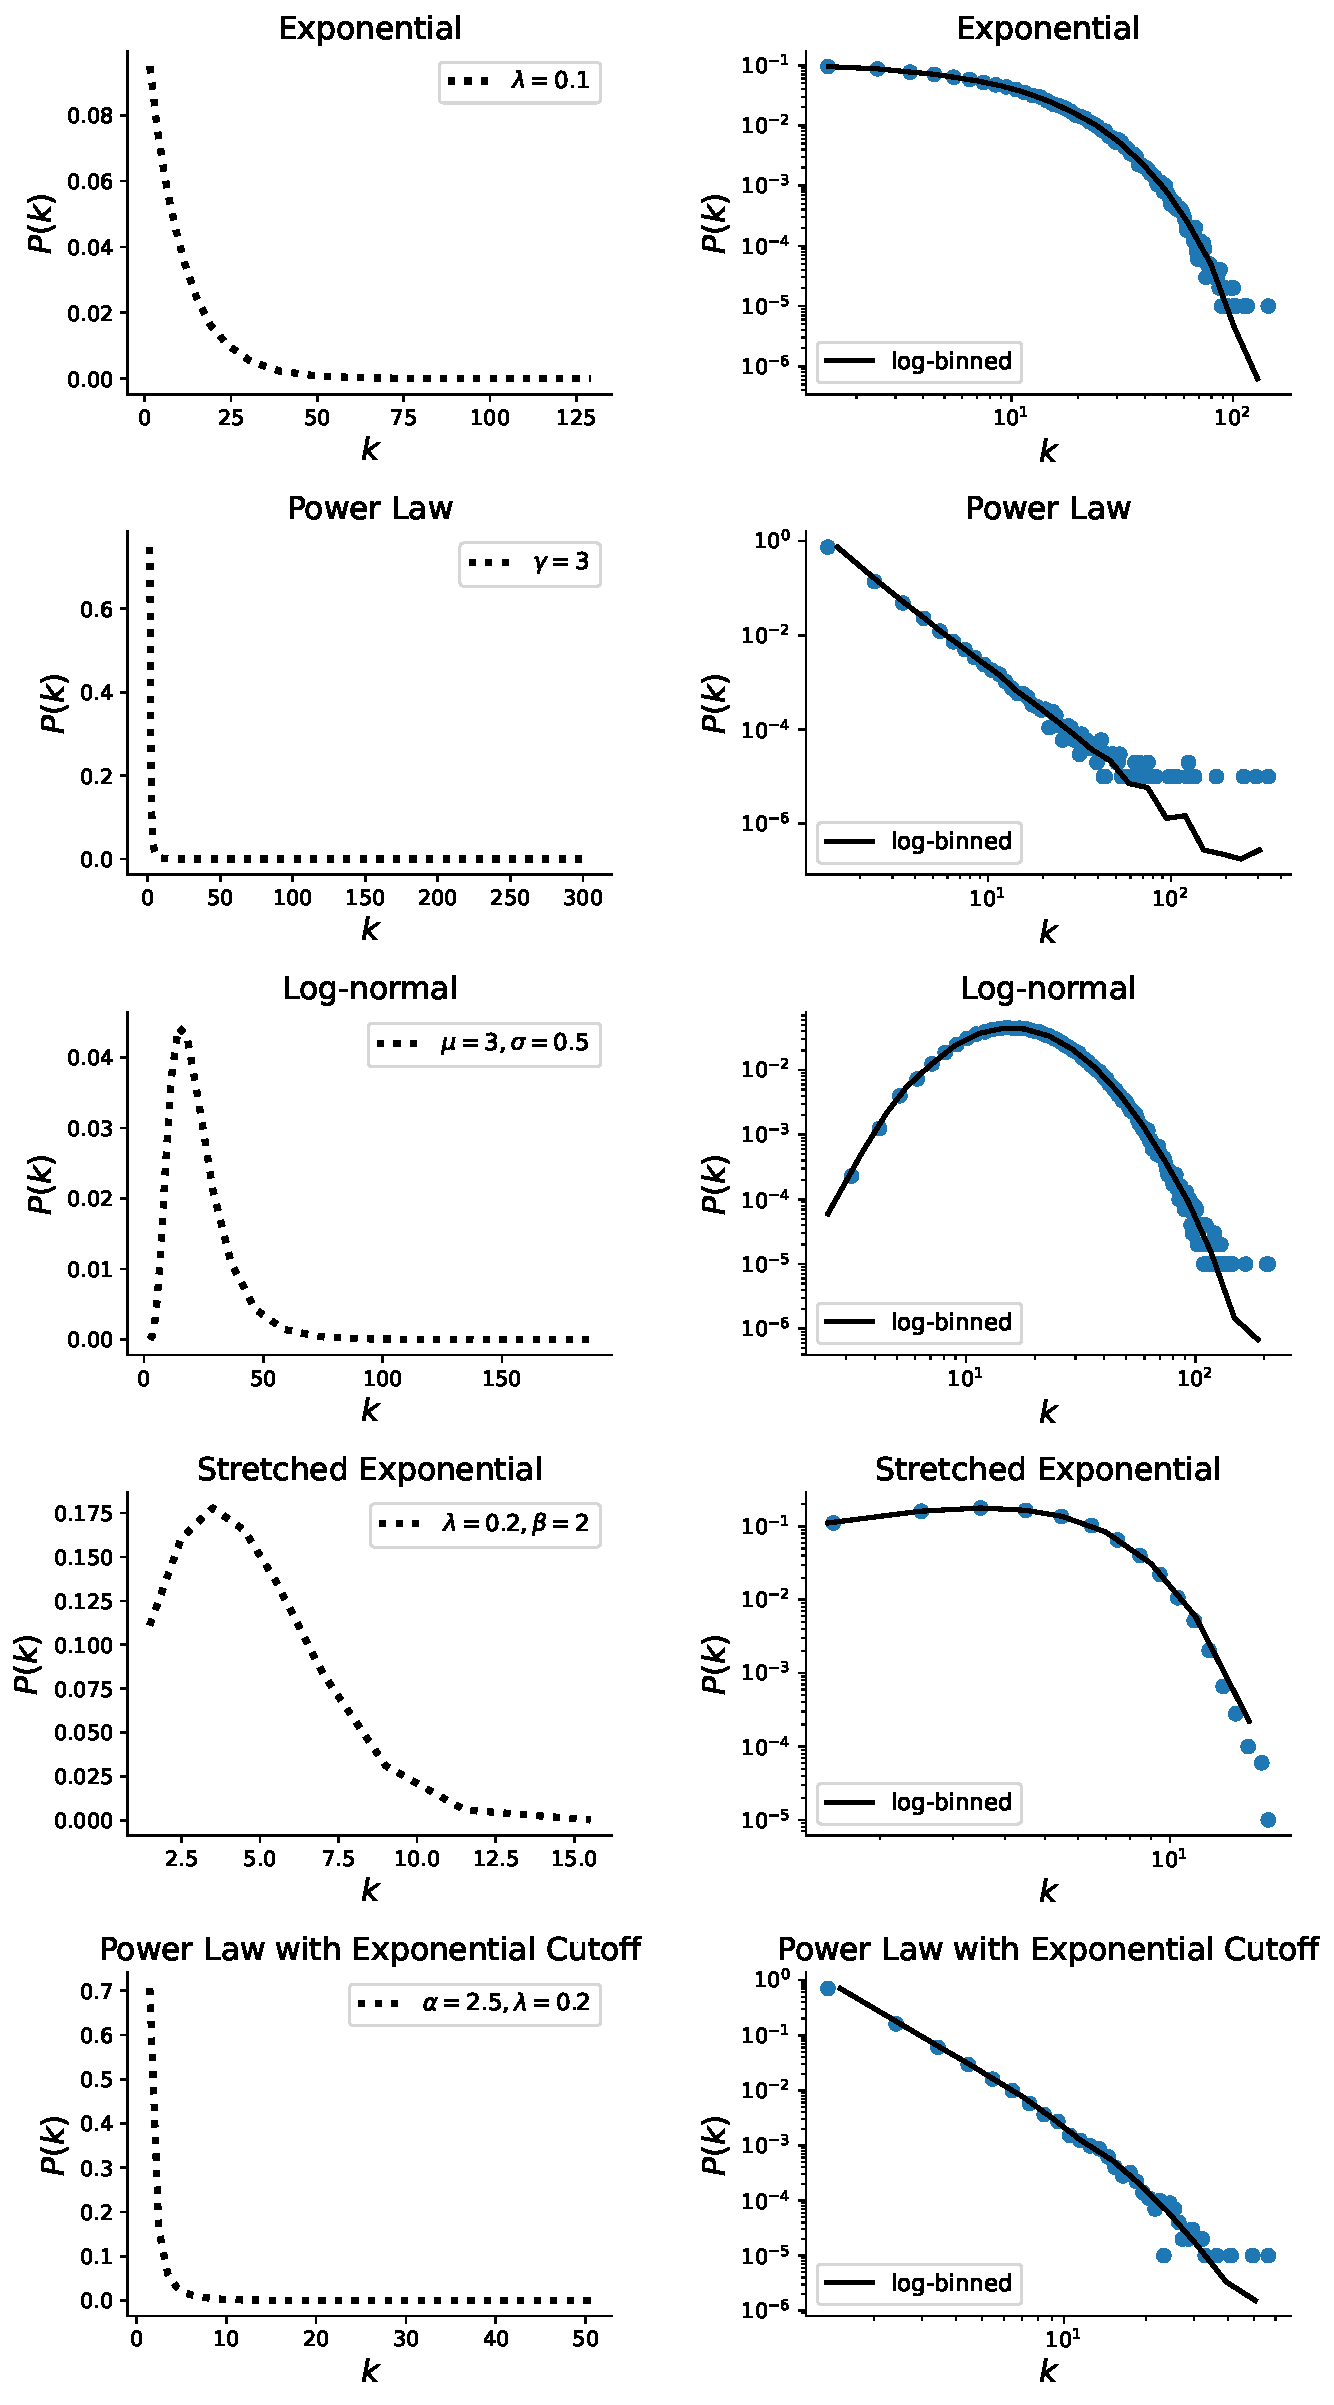
\includegraphics[width=0.75\textwidth]{chapter2/Distributions_plots.pdf}
	\caption{Probability distributions on a linear and double logarithmic scale.}
	\label{fig:distributions}
\end{figure}

\subsection{The properties of distributions}

\textbf{Power-law distribution.} The power-law distribution \cite{mitzenmacher2004brief, newman2005power} is defined as 

\begin{equation}
p(k) = C k^{-\gamma}
\end{equation}
where parameter $\gamma$ is an exponent of the power-law distribution while the C is the normalizing constant. 

The distribution can take discrete and continuous values, defined for positive values $k>0$, so there is a lower bound to the power-law function $k_{min}$. For the discrete case $C=1/\zeta(\gamma, k_{min})$, while in the continuous case $C=(\gamma-1)k_{min}^{\gamma-1}$. 

The power-law distribution is called scale-free distribution. If we scale the value $k$ for the factor $2$, the ratio of $p(x)/p(2x)$ is constant and does not depend on the $k$ \cite{caldarelli2007scalefree}. We'll find that these criteria are not satisfied by any other distribution. 
\begin{equation}
\frac{p(k)}{p(2k)} = \frac{Ak^{-\gamma}}{A(2k)^{-\gamma}} = 2^{\gamma}
\end{equation}

The scale-free function is defined as $p(bx) = g(b)p(x)$. The solution of this equation is $p(x)=p(1)x^{-\gamma}$, where  $\gamma=-p(1)/p^{'}(1)$ leads us to the conclusion that if the function is self-similar, it has to be power-law.



\textbf{Lognormal distribution}. The variable $x$ has the lognormal distribution if the random variable $y=ln(x)$ is distributed as normal distribution \cite{limpert2001log}. 

\begin{equation}
f(y) = \frac{1}{2\pi\sigma}e^{-(y-\mu)^2/2\sigma^2}
\end{equation}
where $\mu$ is the mean, and $\sigma$ is the standard deviation. The density distribution of the lognormal distribution is defined as
\begin{equation}
f(x) = \frac{1}{x \sigma \sqrt{2\pi}}e^{-(log(x)-\mu)^2 /2\sigma^2} 
\end{equation}

The lognormal distribution has finite mean $e^{\mu+1/2\sigma^2}$, and the variance $e^{2\mu+\sigma^2}(e^{\sigma^2 -1})$.  \cite{mitzenmacher2004brief}. Despite the finite moments, the lognormal distribution can be similar to the power-law distribution. If the variance is large, then the probability function on the log-log plot appears linear for a large range of values. 

Using the \textbf{multiplicative processes}, we can generate the lognormal distribution \cite{caldarelli2007scalefree, mitzenmacher2004brief}. The lognormal distribution is generated by processes that economist Gibrat called the law of proportionate effect. If we start from the organism of size $S_0$. At each time step, the organism may grow or shrink according to the random variable $\epsilon$, 
\begin{equation}
S_t = \epsilon_t S_{t-1}
\end{equation}

When the system's state at time t is proportional to the state at the previous time step, we have the multiplicative process. The $\epsilon$ is a proportionality constant that can change over time. The current state depends only on the initial size $S_0$ and the $\epsilon$ variables.:
\begin{equation}
S_t = \epsilon_t S_{t-1} = \epsilon_t \epsilon_{t-1}... \epsilon_2 \epsilon_1 S_{0}
\end{equation}

If $\epsilon_t$ is drawn from the lognormal distribution, then $S_t$ also follows lognormal, as the product of lognormal distributions is again lognormal. Still, the $\epsilon$ distribution does not determine the distribution of the $S_t$. Taking the logarithm of the equation:
\begin{equation}
ln(S_t) = ln(S_0) + \sum_{i=0}^{t} ln(\epsilon_i)
\end{equation}

The sum of the logarithms of the $\epsilon_t$, according to the Central Limit Theorem (CLT), follows the normal distribution. The CLT states that the sum of identically distributed random variables with finite variance converges to the normal distribution. If $ln(S_t)$ is normally distributed, then $S_t$ follows the lognormal distribution.   

The multiplicative processes generate the lognormal distribution. Introducing a threshold in the multiplicative process leads to the power law. For example, in the Champernowne model \cite{caldarelli2007scalefree}, individuals are divided into classes according to their income. The minimum income is m. People between incomes m and $\gamma m$ are in the first class, and the second class are people with incomes between $\gamma m$ and $\gamma^2 m $. The individuals can change their class, so it is described as a multiplicative process, but with a threshold, as income can not be lower than m. If we fix $\gamma=2$, and consider that with probability $p_{i,i-1}=2/3$, the change is from higher to lower class. In contrast, with probability, $p_{i, i+1}=1/3$ individual goes to a higher class. In this process, the distribution of incomes emerges as the power-law distribution.



\textbf{Power law with exponential cutoff}. The density function has the following form 
\begin{equation}
p(k) = C k^{-\gamma}e^{-\lambda k}
\end{equation}
where $k>0$ and $\gamma>0$. This function combines the power-law, and exponential terms responsible for an exponentially bounded tail \cite{barabasi2016network}. Taking the logarithm $ln(p(k)) = lnC - \gamma lnk - \lambda k$, when $k<<1/\lambda$ the second term dominates, so distribution follows the power-law, with exponent $\gamma$. Otherwise, the $\lambda x$ term dominates, resulting in an exponential cutoff for high values. 

\textbf{Streched exponential} The stretched exponential distribution is defined as:
\begin{equation}
p(k) = c k^{\beta - 1}e^{-(\lambda k)^{\beta}}
\end{equation}
the parameter $\beta$ is stretching exponent determining the properties of the function $p(k)$ \cite{barabasi2016network}. For $\beta=1$, the function is exponential. For $\beta<1$, it is hard to distinguish the distribution from the power law. We have a compressed exponential function for $\beta>1$, so $k$ varies in the narrow range. 

%\subsection{Plotting the distributions}
%%TODO ovo ne treba da bude deo teze

%The first step in analyzing the empirical data is to create the frequency plot or histogram. Data are binned in equal intervals, and the number of data points within the interval are plotted. It is hard to determine whether the distribution is exponential or power law when plotting heavy-tailed distributions \cite{caldarelli2007scalefree}. If data are from power law distribution on the double logarithmic scale, they will look linear:
%\begin{equation}
%log p(k) = \gamma log(k) + c
%\end{equation}  
%On the log-log scale, we notice that noise in the tail of the distribution data exists. As the size of the bins is constant, the bins' density for large values also becomes large. To avoid the fluctuations in the tail, we can use logarithmic binning \cite{barabasi2014network, caldarelli2007scalefree, nair2022fundamentals}. The noise is reduced by dividing the $x$ axis into $n$ bins $b_n = c^n$, so the following bin is wider than the previous one. For the base $c$, we can choose any value $c>1$. Similarly, the binning can take the following form $b_n = k_0\exp{(cn)}$, where $k_0$ is the minimum data point, while the $c$ is the arbitrary base. All data points between values $[b_n, b_{n+1})$ are represented with one point $p(k_n) = N_n/b_n$, where $N_n$ is the number of nodes found in the bin $b_n$ and $k_n = \sum_i k_i / N_n$ is the average degree of the nodes in the bin $b_n$. By averaging over bins in the tail, noise in the tail of the distribution is reduced. Still, no matter how the bin size is chosen, the information about original data points is lost, especially in the distribution tail where bins are larger and include more samples. Figure \ref{fig:distributions} shows how different distributions look on linear (first column) and log-log scale (second column).



%Instead of plotting the probability distribution, it is possible to calculate the cumulative distribution, defined as $P(k) = \int_{k}^{\infty} p(k^{'}) dk^{'}$ for continuous function or as $P(k)=\sum_{k^{'}=1}^{k}p(k^{'})$ for the discrete function. For example, the CDF function for power law is also a power-law function but with exponent $\gamma -1$: $P(k)= k^{-(\gamma-1)}$. Note that for cumulative distribution, it is not necessary to use log-binning.

\subsection{Estimating the distribution parameters}

The maximum likelihood estimation(MLE) is a method where we consider that data comes from a particular distribution, so we want to maximize the likelihood of the data to find the distribution parameters. For a given set of i.i.d. observations $x_1, x_2, ...x_n$, sampled from the distribution $p(x)$, we can define the likelihood function  \cite{nair2022fundamentals}. The likelihood function tells us how likely it is to have the given data if the distribution parameters are $\theta$. 

\begin{equation}
L (\theta| x_1, ... x_n) = \prod_{i=1}^{i=n} p(x_i | \theta)
\end{equation}

The parameter that maximizes the likelihood function is $\theta_{max} \in arg max L(\theta| x_1,... x_n)$.

We can solve the equation and derive the expression for maximum likelihood parameters. The parameters can be obtained with numerical optimization for distributions where an analytical solution is unavailable. In practice is much easier to work with the logarithm of the likelihood function, $log(L) = \sum_{i=1}^{i=N} p(\theta| x_i)$, because then the product changes to summation. For the power-law distribution, the exponent is calculated as  
$\gamma = 1+n[\sum ln \frac{k_i}{k_{min}} ]^{-1}$. For a discrete distribution, the solution may be obtained by optimizing the log-likelihood function $log(L) = log\prod_{i=1}^{n} \frac{k_i^{-\gamma}}{\zeta(\gamma, k_{min})}$.

We can use the MLE \cite{clauset2009power} method to fit any distribution to the data. Even if obtained distribution looks like a power law, and some parameters are estimated, it does not have to be that data are truly from the power-law distribution. With the MLE method alone, it is impossible to distinguish between different distributions, and we do not know how accurate the obtained results are. To determine the quality of the fit, we need to use another statistical method called the \textbf{goodness-of-the-fit} test. The main idea is based on calculating the distance between distributions of empirical data and the model using Kolmogorov-Smirnov statistics. The Kolmogorov Smirnov statistics is the maximum distance between the CDF of the data and the fitted model, $D = max |S(x) - P(x)|$.

First, we fit empirical data to get model parameters and calculate the KS statistics of this fit \cite{clauset2009power}. Then, many synthetic data sets are generated with model-optimized model parameters. Then each synthetic data set is fitted, and KS statistics are obtained relative to its model. From there, we can calculate \textbf{p-value}, the fraction of times that KS-statistics in synthetic distributions is larger than in empirical data.  If $p-value<0.1$, we reject the hypothesis that this distribution describes the empirical data. Otherwise, the model can not be rejected. Failing to reject the hypothesis does not mean the model is a correct distribution for the data. Other distributions might fit the data equally good or even better. To have an accurate p-value, we need a large sample. For a small number of synthetic distributions, it is possible to have a high p-value, even if the distribution is the wrong model for the data. Finally, we need to be confident in obtained results. The same procedure can be repeated for different distributions. If the p-value for the power law is high, while for alternative distribution, it is low, we can conclude that the power law is a more probable fit. 

Another method, the \textbf{likelihood ratio test}, allows us to compare two distributions directly \cite{clauset2009power}. The distribution with a higher likelihood under empirical data is a better fit. We can calculate the likelihood ratio, or it is easier to obtain the likelihood ratio's logarithm because its sign determines which distribution is a better fit. For given two distributions $p_1(x)$and $p_2(x)$. 

The likelihoods are defined as $L_1=\prod_{i=1}^{n}p_1(x)$ and $L_2=\prod_{i=1}^{n}p_2(x)$, or the ratio of likelihoods as $R=\frac{L_1}{L_2} = \prod_{i=1}^{n} \frac{p_1(x)}{p_2(x)}$. Taking the logarithm, we obtain the log-likelihood ratio

\begin{equation}
\mathcal{R} = \sum_{i=1}^{n} \left[log p_1(x_i) - log p_2(x_i)\right]
\end{equation}

As data $x_i$ are independent, by central limit theorem, their sum $\mathcal{R}$ becomes normally distributed, with expected variance $\sigma^2$. We can approximate the variance as 

$$\sigma^2 = \frac{1}{n}\sum_{1}^{n}[(l_i - l_i) - (<l>^{(1)}- <l>^{(2)})]$$

When $R>0$, the first distribution is a better fit to the data, and then $R<0$, the other one should be chosen. When $R=0$, it is not possible to distinguish between two distributions. The sign of $R$ is not enough criteria to conclude which distribution is a better fit, and it is a random variable subject to statistical fluctuations. We need a log-likelihood ratio that is sufficiently positive or negative to ensure that its sign does not result from fluctuations.

If we are suspected that the expectation value of the log-likelihood ratio is zero, the observed sign of $\mathcal {} $ is simply the product of fluctuations and can not be trusted. The probability that the measured log-likelihood ratio has a magnitude as large or larger than the observed value R is given as

\begin{equation}
p = \frac{1}{\sqrt{2\pi n \sigma^2}} \int_{-\infty}^{-|\mathcal{R}|}e^{-x^2/2n\sigma^2}dx + \int_{|\mathcal{R}|}^{\infty}e^{-x^2/2n\sigma^2}dx
\end{equation}

Here we use the standard two-tail hypothesis test \cite{clauset2009power}, assuming that the null hypothesis is  $R= 0$. If the p-value is larger than a threshold, the R sign is unreliable, and the test does not favour any distribution. If p is small, $p<0.1$, then it is unlikely that the observed sign is obtained by chance, so we reject the null hypothesis that $R=0$. 
%\newpage

\section{Network models}
%%TODO Ovde treba ubaciti samo jedan pasus zasto su nam bitni modeli. Cemu sluze, zasto ih pravimo i slicno.

The interest in analyzing real-world networks allowed us to describe their statistical properties and formulate models that can explain essential features in the data. With network models we can understand the origins of the properties of the complex networks, what mechanisms influence the generation of the network and how network properties emerge. In this section are considered random network model and small-world model, which are static models, as the number of nodes are fixed. Even though random network is not applicable on the real networks it is important historically as one of the first network models. The small-world model explains how properties of real networks such as high clustering and small distances may emerge. On the other hand, generative models, as models of preferential attachment, where network grows according to specific growing rules are important for understanding how network structure is created. They allow as to explore different growing mechanisms and comparing obtained networks with real data we can conclude which growth processes have influence on the network structure.     

\subsection{Random network model}

The random graph model was introduced by mathematicians Paul Erdős and Alfred R\' {e}nyi in 1959. In this model, connections between nodes are chosen randomly, and every link has the same probability of existing. The graph is characterized only by a number of the nodes $N$ and the linking probability $p$, so Erdős-R\' {e}nyi graph is written as $G(n, p)$. 

The creation of ER random network consists of the following steps:
\begin{itemize}
	\item we start with $N$ isolated nodes
	\item between each $N(N-1)/2$ pair of nodes we create link with probability $p$; sampling random number $r \in (0,1)$, we create link if $r \leq p$    
\end{itemize}


\begin{figure}[H]
	\centering
	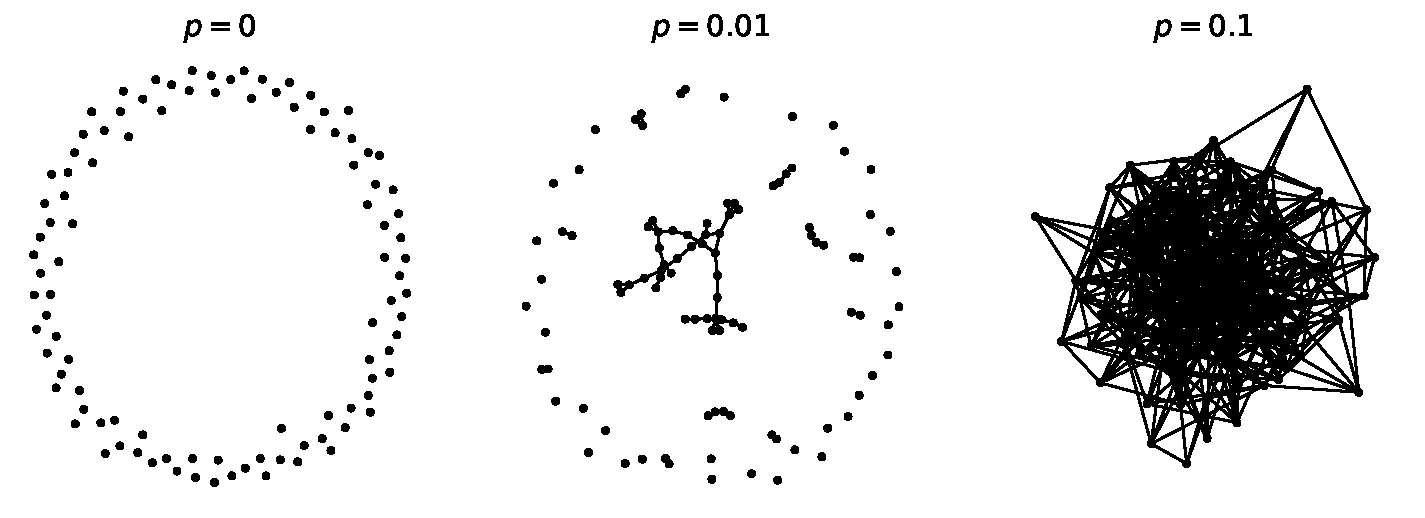
\includegraphics[width=0.9\linewidth]{chapter2/ERgraph.pdf}
	\caption[Erdős-R\' {e}nyi]{Erdős-R\' {e}nyi graph with $N=100$ nodes and different linking probabilities $p$.}
	\label{fig:erp}
\end{figure}

We should note that this process is stochastic. The networks $G(N, p)$ with the same parameters do not need to have the same structure; i.e. they differ in the number of links. Therefore, the single random graph is only one of all the possible realizations in the statistical ensemble. 

Two simple quantities that could be estimated are the average number of links and the average degree. For a complete graph with $N$ nodes, the number of edges is $N(N-1)/2$. As the probability of drawing every edge is $p$, the \textbf{average number of links} is given as 

\begin{equation}
\langle L \rangle = \frac{N(N-1)}{2}p
\end{equation}

We conclude that the network's density equals probability $p$.
The \textbf{average degree} is approximated as $\langle k \rangle = 2 \langle L \rangle / N $, leading to:

\begin{equation}
\langle k \rangle = (N-1)p 
\end{equation}

The \textbf{degree distribution} of ER random graph follows the binomial distribution \cite{barabasi2016network}. 

\begin{equation}
P(k) = \binom{N-1}{k}p^k(1-p)^{N-1-k}
\end{equation}

The probability that the node has degree $k$ is given with the second term $p^k$, while the probability that other N-1-k links are not created is given with the third part of the equation. Finally, there are  $\binom{N-1}{k}$ combinations for one node to have $k$ links from $N-1$ possible links. 

The binomial distribution describes very well small networks, see Figure \ref{fig:erdist}. For larger networks, we find that they are sparse and that the average degree is much smaller than a number of nodes $\langle k \rangle << N$. In this limit, binomial distribution becomes the Poisson, as could be shown on Figure \ref{fig:erdist} which now depends only on one parameter $\langle k \rangle$

%%TODO pozvati se na sliku
%%TODO ispraviti naziv na slici

\begin{equation}
p(k) = \frac{1}{k!}e^{-\langle k \rangle}\langle k \rangle^{k}.
\end{equation}

\begin{figure}[H]
	\centering
	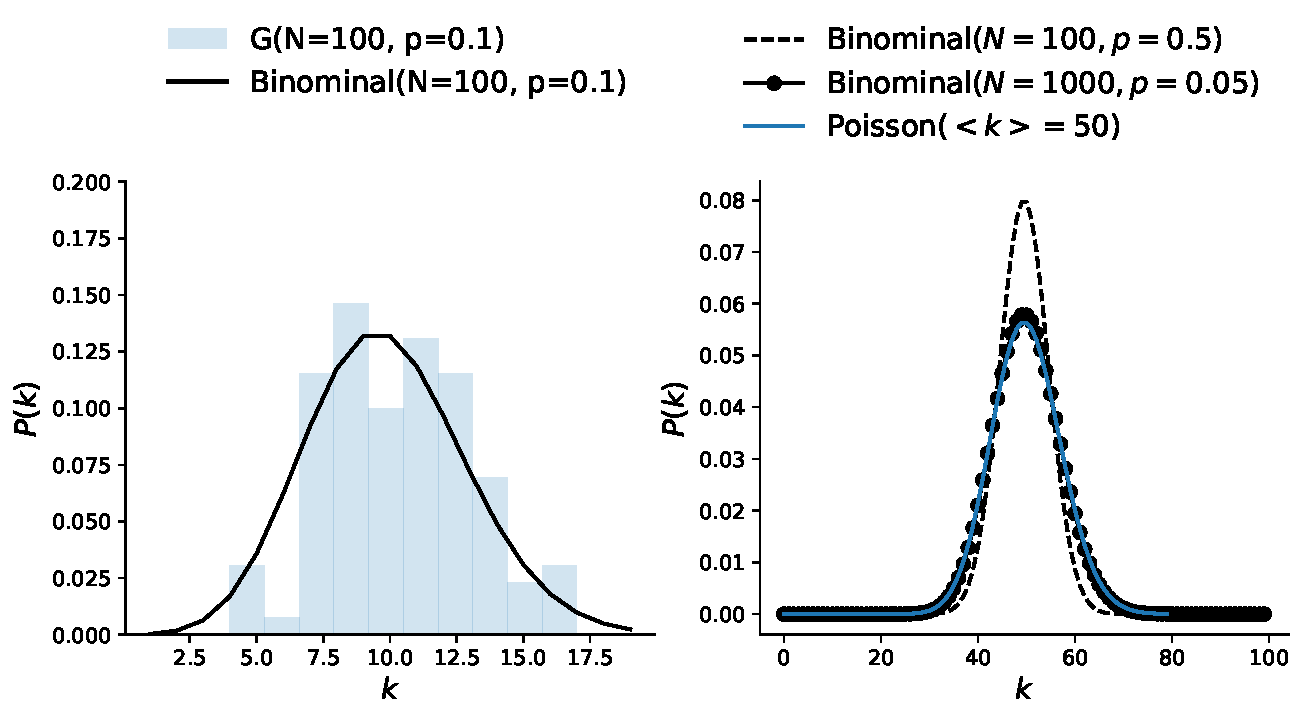
\includegraphics[width=0.9\linewidth]{chapter2/ER_dist.pdf}
	\caption[Degree distribution of Erdős-R\' {e}nyi graph.]{Degree distribution of ER graph. The degree distribution of small networks follows binomial. Larger networks are better approximated with Poison distribution, and degree distribution for fixed average degree $<k>$ becomes independent of the network size.}
	\label{fig:erdist}
\end{figure}

The random graph has a very small \textbf{average path length}, it is given as $\langle l \rangle = \frac{ln N}{ln(pN)}$ that is characteristic of many large networks \cite{bollobas2003mathematical}. The clustering coefficient is proportional to linking probability, $\langle C \rangle = p$, so we find a small clustering coefficient in large random networks, contrary to real-world networks.  %about small networks Barabasi chapter3, page 22

Figure \ref{fig:erp} shows how the network becomes more connected by increasing the linking probability $p$. When $p=0$, all nodes are disconnected. In the other limit, $p=1$, the network is fully connected. Between those two probabilities exists critical probability, where the giant component appears. The giant component is a sub-graph whose size is proportional to the network size. In other words, the network does not have disconnected components. Such change in the network is a phase transition in network connectivity and is related to percolation theory. 

The phase transition occurs when the average degree is $ \langle k  \rangle = 1$, which gives us: $p_c = \frac{1}{N-1}$, meaning that all nodes have degree larger than one \cite{barabasi2016network}. When the $ \langle k  \rangle < 1$, the network is in the sub-critical regime where all components are small. In the critical regime, the size of the giant component is proportional to the $N^{2/3}$. In the supercritical regime, $ \langle k  \rangle > 1$, the probability of a giant component appearing is 1.

\subsection{Small-world networks}

Inspired by the idea that real-world networks are highly clustered, and the average distance is small, Watts and Strogatz \cite{watts1998collective} proposed the "small-world" model. The model starts from the regular lattice, and with rewiring links, the network starts to resemble small-world property. The procedure is the following:

\begin{itemize}
	\item At the beginning, nodes are placed on the ring lattice, see Figure \ref{fig:wsgraph}, and each node is connected to $k/2$ first neighbours on the left and the right side. Initially, the clustering coefficient is high, $c=3/4$. 
	\item For each link in the network, with probability $p$, we choose a random node to rewire the link. This makes long-distance nodes connect, decreasing the network's average path length, Figure \ref{fig:wsgraph}.
\end{itemize}

The model interpolates between the regular graph when the probability is $p=0$ and the random graph with $p=1$ when all links are randomly rewired. Short distances and high clustering are present in the network  for the relatively small probabilities ranging from $p \approx 0.01 - 0.1$ \cite{watts1998collective}. %%TODO kolika je verovatnoca

\begin{figure}[H]
	\centering
	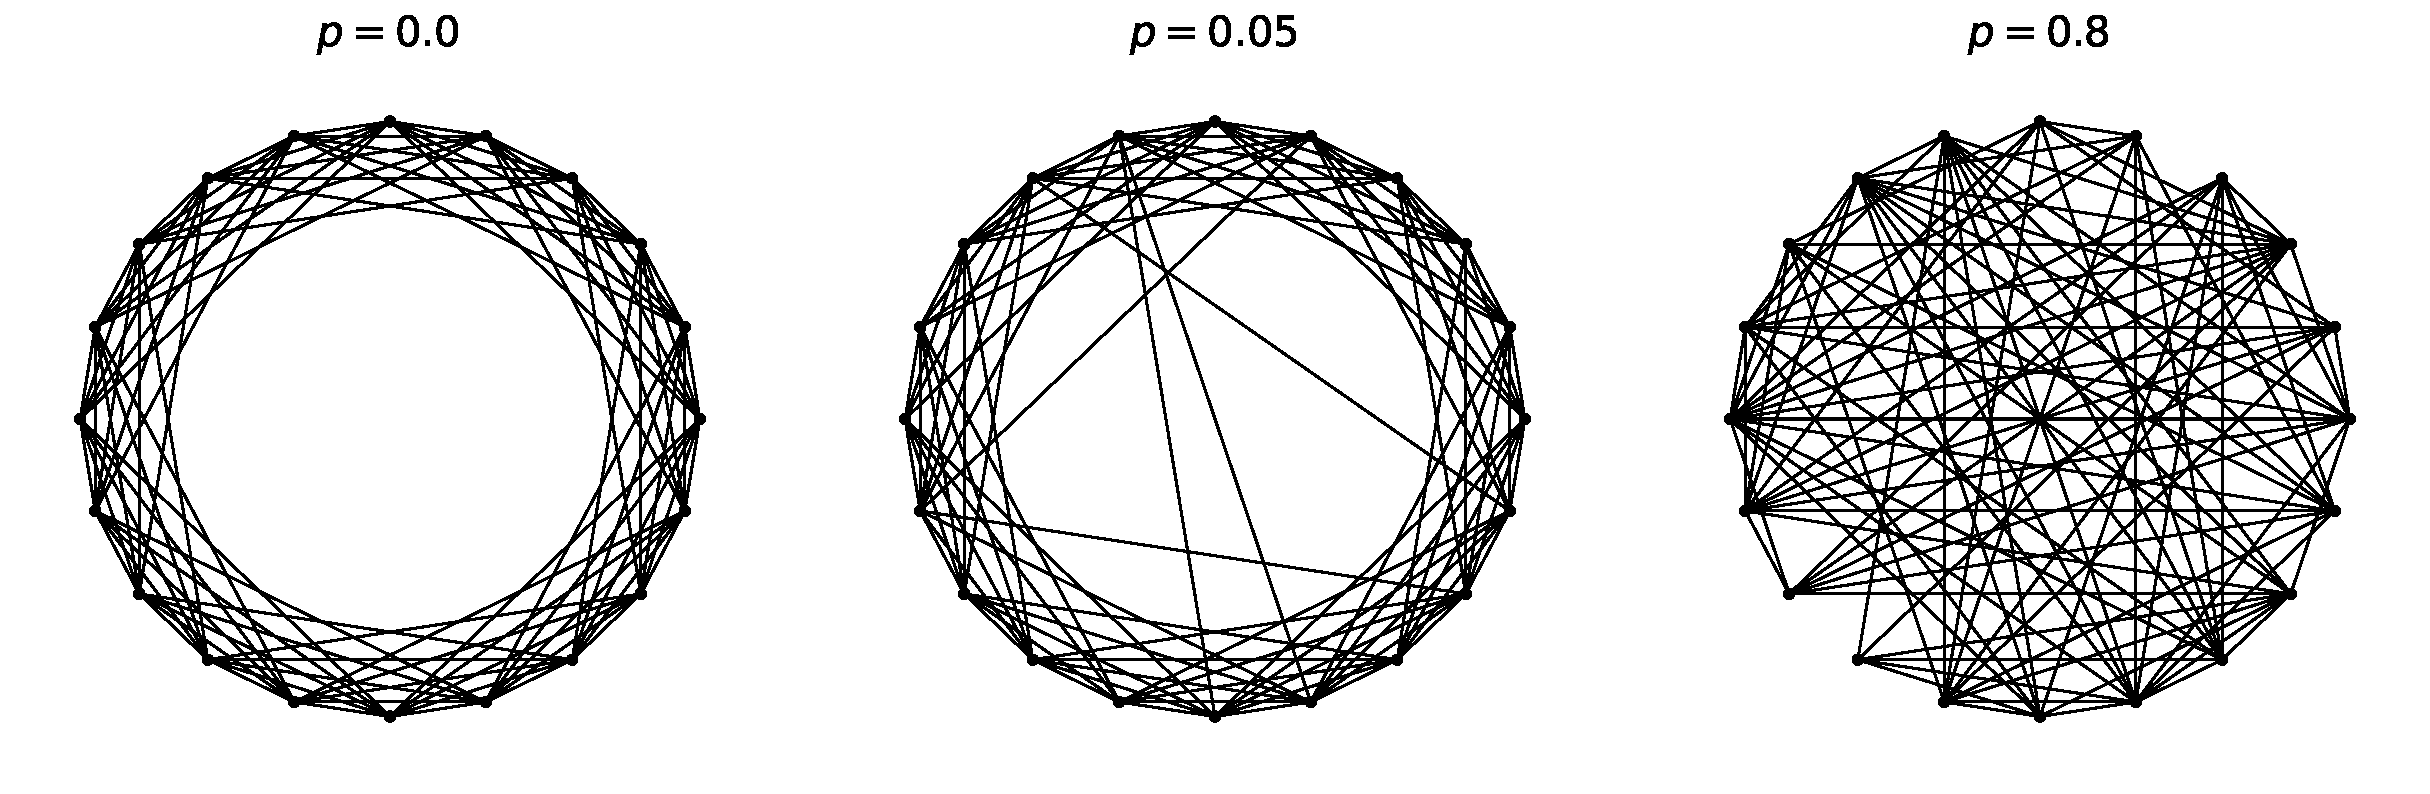
\includegraphics[width=1\linewidth]{chapter2/WS_model.pdf}
	\caption[Watts and Strogatz graph model creation]{Watts and Strogatz graph model creation, for different rewiring probabilities.}
	\label{fig:wsgraph}
\end{figure}

Even though the small-world network model lacks the power-law degree distribution found in real-world networks, it is an important model that motivated the research on random graphs. 

\subsection{Barab\' {a}si-Albert model}

The ER random graph model and WS small-world model are static models where the number of nodes is fixed. It is one of the reasons why they can not fully explain the properties of real systems. The size of real systems does not remain constant; real networks grow. Growth means that at each time step, new nodes are added to the network. The simplest model that produces scale-free networks is the Barabasi-Albert model \cite{barabasi1999}.

\begin{itemize}
	\item The model starts from the small number, $n_0$ randomly connected nodes, with $m_0$ links.
	\item At each time step, a new node with $m$ links joins the network. A new node creates links with the nodes already present in the network, following the linking rules; in this case, preferential attachment rules. 
\end{itemize}

The preferential attachment is important for generating a system with scale-free properties. In the real system, the linking between nodes is not a random process; the preference for specific types of nodes exists. For example, popular web pages can quickly get more visits, or it is expected that already popular papers will get more citations. This effect is also called rich-get-richer or preferential attachment.

The simplest formulation of the preferential attachment model is that new nodes tend to connect with high-degree nodes. The linking probability $\Pi$ is then proportional to node degree $k$:  

\begin{equation}
\Pi(k_i) = \frac{k_i}{\sum_jk_j} 
\end{equation} 

As at each step one node arrives, we can estimate the number of nodes at the time step t, $N(t) = n_0+t$, with links $L(t) =m_0+ mt$. 

First, we can calculate the evolution of network degrees in time.
\begin{equation}
\frac{dk_i}{dt} = m\Pi(k_i) = m\frac{k_i}{\sum_jk_j} = m\frac{k_i}{m_0 + 2mt}
\end{equation}

Note that the new node that arrived at time point $t_i$ has degree $m$, as it links to $m$ old nodes. Solving the equation, we get that at $t>t_i$, it has a degree that grows as the square root of time; it also shows that younger nodes easily acquire a larger degree. 
\begin{equation}
k_i(t) = m \left(\frac{t}{t_i}\right)^{\frac{1}{2}}
\end{equation}

With this equation we can calculate the probability that node has degree smaller than k  as \\ $P[k_i(t)<k] = P(t_i > \frac{m^{1/\beta}t}{k^{1/\beta}})$. Assuming that we add nodes in constant time intervals we have $P(t_i) = 1/(m_0+t)$. The cumulative probability is then  $P(t_i>\frac{m^{1/\beta t}}{k^{1/\beta}}) = 1 - \frac{t}{t+m_0}\left(\frac{m}{k}\right)^{1/\beta} $.
Finally, the degree distribution has following form
\begin{equation}
P(k) = \frac{\partial P[k_i(t)<k]}{ \partial k} \sim 2m^2 k^{-3} 
\end{equation}

\textbf{Degree distribution follows power-law}, and for large k is approximated with $P(k) = k^{-\gamma}$, where $\gamma=3$. As the network grows, nodes with larger degrees become bigger and we end up with few nodes with many links, called hubs. Figure \ref{fig:bamodel} - left pane shows generated BA network, consisting of $N=100$ nodes, where even on this scale we can notice emergence of hubs. The right pane of Figure \ref{fig:bamodel} shows obtained degree distribution of larger network with $N=10^4$ nodes. Degree distribution is also independent of the time and size of the system, meaning the emergence of a stationary scale-free state.  If we vary $m$, the slope of distributions is the same, but they are parallel. After rescaling $p(k)/m^2$, they fall on the same line \cite{barabasi2016network}.  

\begin{figure}[h]
	\centering
	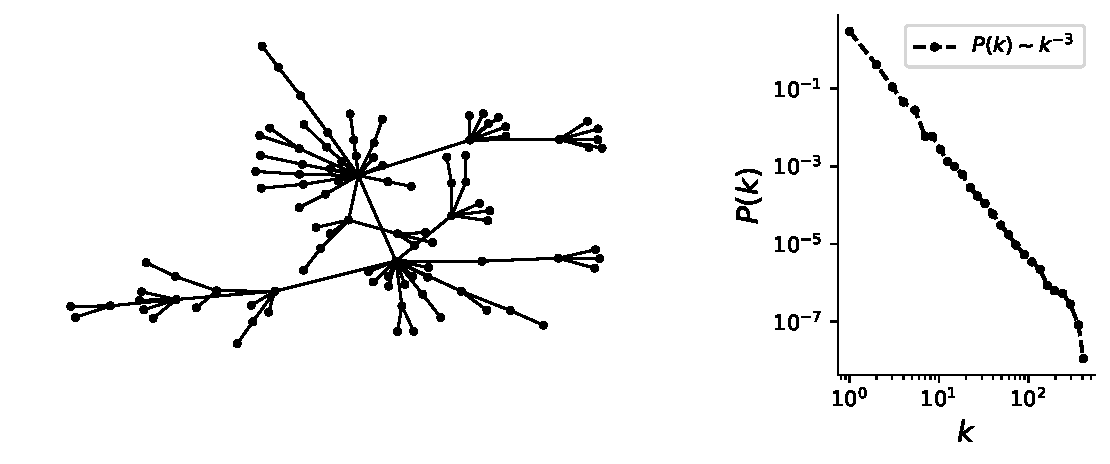
\includegraphics[width=1\linewidth]{chapter2/BAmodel.pdf}
	\caption[Barabasi-Albert model]{Barabasi-Alber model. The left panel shows the BA network, with 100 nodes. The right panel shows the degree distribution for BA network of $10^4$ nodes, that follows power-law.}
	\label{fig:bamodel}
\end{figure}

%More precisely, the degree distribution has form \cite{krapivsky2010kinetic}:
%\begin{equation}
%P(k) = \frac{2m(m+1)}{k(k+1)(k+2)} \sim k^{-3}.
%\end{equation}
%For large $k$, it is exactly the power law, as shown in Figure \ref{fig:bamodel} . 
%Distributions do not depend on the N.
%% TODO Glavna karakteristika BA modela je power-law degree distribution, To ovde nije ni priblizno ocigledno. Bilo bi lepo da postoji i slika., 
%%TODO dodati izvodjenje -OVO MOZDA

%stationary degree distribution does not depend on the system parameters, so different systems have similar behaviour
%As the network grows, nodes with larger degrees become bigger, so we end up with few nodes with many links, called hubs.
 
The \textbf{network diameter}, represents the maximum distance in network, $d \sim \frac{lnN}{lnlnN}$ \cite{bollobas2003mathematical}. The diameter grows slower than $lnN$, making the distances in the BA model smaller than in the random graph. The difference is found for large N. It is known that the BA network has hubs that shorten the path between less connected nodes. Also, if hubs are removed from the network, the network easily partitions into several components, losing its properties. The \textbf{clustering coefficient} of the BA model follows $C \sim \frac{ln N^2}{N}$ \cite{bollobas2003mathematical}. It differs from clustering found in random networks, and BA networks are generally more clustered. 

The combination of the growth and preferential attachment linking is crucial for getting scale-free networks \cite{barabasi1999}. For example, eliminating the preferential attachment; in a growing network with random linking, degree distribution is stationary but follows exponential. In contrast, the absence of growth leads to the non-stationary degree distribution. When a number of nodes is fixed, the network grows only in the number of links, such that randomly chosen node $i$ connects to node $j$ according to probability $\Pi$. In the beginning, the degree distribution follows the power law, the same as in the BA model. As more links are added to the network, the distribution changes its shape; first, the peak appears, while at the end network becomes a complete graph, where all nodes have the same degree.  

\subsection{Nonlinear preferential attachment model}

In the nonlinear preferential attachment model linking probability also depends on the node degree. The dependence is not linear and has the following a form \cite{krapivsky2001}:

\begin{equation}
\Pi(k_i) = {k_i}^{\beta}
\end{equation} 

The probability that a newly added node attaches to node $i$ depends on the existing $i$-th node degree $k_i$ and the parameter $\beta$. When $\beta=1$, the model is the BA model, where degree distribution follows the power law. When $\beta=0$, linking probability becomes uniform; i.e. it corresponds to a random network model, and the degree distribution is Poisson; there is exponential decay. 

For $\beta>1$, preferential attachment effects are increased, leading to super hubs' emergence. The hub-and-spoke network appears in this regime, where almost all nodes are connected to a few high-degree nodes \cite{krapivsky2001}. %OVDE CITIRATI kRAPIVSKY REDNER RADOVE

On the other hand, if $\beta<1$, the model is in a so-called sub-linear preferential attachment regime. The linking probability is not random, so degree distribution does not follow Poisson, but also, the preference toward high-degree nodes is too weak for having the pure power law. Instead, degree distribution converges to stretched exponential.


\subsection{Aging model}

To understand how aging can impact the network structure, we look into probability dependent on two parameters, nodes degree $k$ and age of node $i$ at the time point $t$ $\tau_i=(t-t_i)$, where $t_i$ is the time when node $i$ is added to the network \cite{dorogovtsev2000b}. 
\begin{equation}
\Pi_{i}(t)\sim k_{i}\tau_{i}^{\alpha} 
\label{eq:aging}
\end{equation}

The parameter $\alpha$ controls the linking probability dependence on the nodes' age; if $\alpha=0$, the ageing of nodes is disregarded. 

If $\alpha>0$ is positive, the older nodes are more likely to create connections. In this regime, the preferential attachment stays present, and the high-degree and older nodes are preferred. For very high $\alpha$, each node is connected to the oldest node in the network. The scale-free properties are present; the power-law exponent $\gamma$ deviates from $\gamma=3$. It is found that $\gamma$ ranges between $2$ and $3$. 

When $\alpha$ is negative, ageing overcomes the role of preferential attachment, and scale-free properties are lost. For significant negative $\alpha$ network becomes a chain; the youngest nodes are those who get connected. 

\begin{figure}[h]
	\centering
	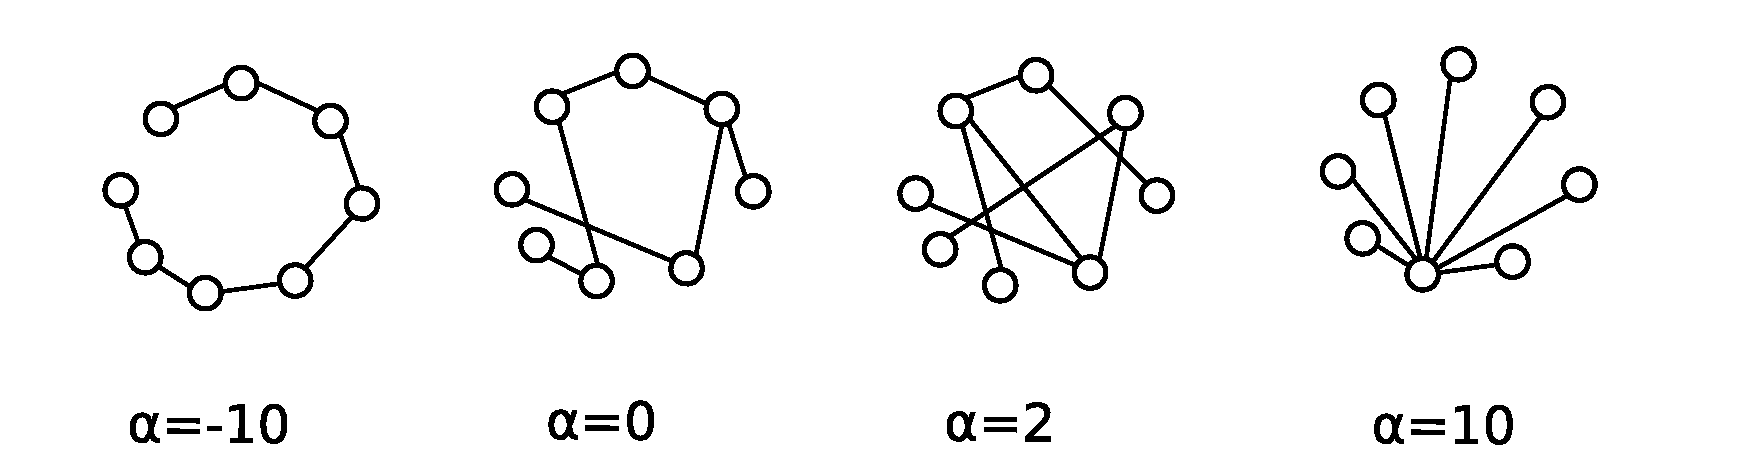
\includegraphics[width=1\linewidth]{chapter2/aging_model.pdf}
	\caption[Aging model]{Aging model}
	\label{fig:aging}
\end{figure}

In the general ageing model, the non-linearity on the node degree is introduced, so this model has two tunable parameters $\alpha $ and $\beta$. The probability that a link is created between the new node and the existing node is defined as \cite{hajra2004}

\begin{equation}
\Pi_{i}(t)\sim k_{i}(t)^{\beta}\tau_{i}^{\alpha} 
\label{eq:1}
\end{equation}

As before, depending on model parameters network evolves into different structures:  
\begin{itemize}
	\item For example if we fix $\beta=1$ and $\alpha=0$ generated networks are scale-free; degree distribution is $P(k) \sim k^{-\gamma}$ with $\gamma=3$.
	\item In the case of nonlinear preferential attachment $\beta \neq 1$ and $\alpha=0$ scale-free properties disappear. 
	\item Scale-free property can be produced along the critical line $\beta(\alpha^{*})$ in the $\alpha-\beta$ phase diagram, see Figure \ref{fig:diagram}.
	
	\item For $\alpha>\alpha^{*}$ networks have \textbf{gel-like small world} behavior.
	
	\item For $\alpha<\alpha^{*}$ and near critical line $\beta(\alpha^{*})$ degree distribution has \textbf{stretched exponential} shape
	
\end{itemize}

\begin{figure}[h]
	\centering
	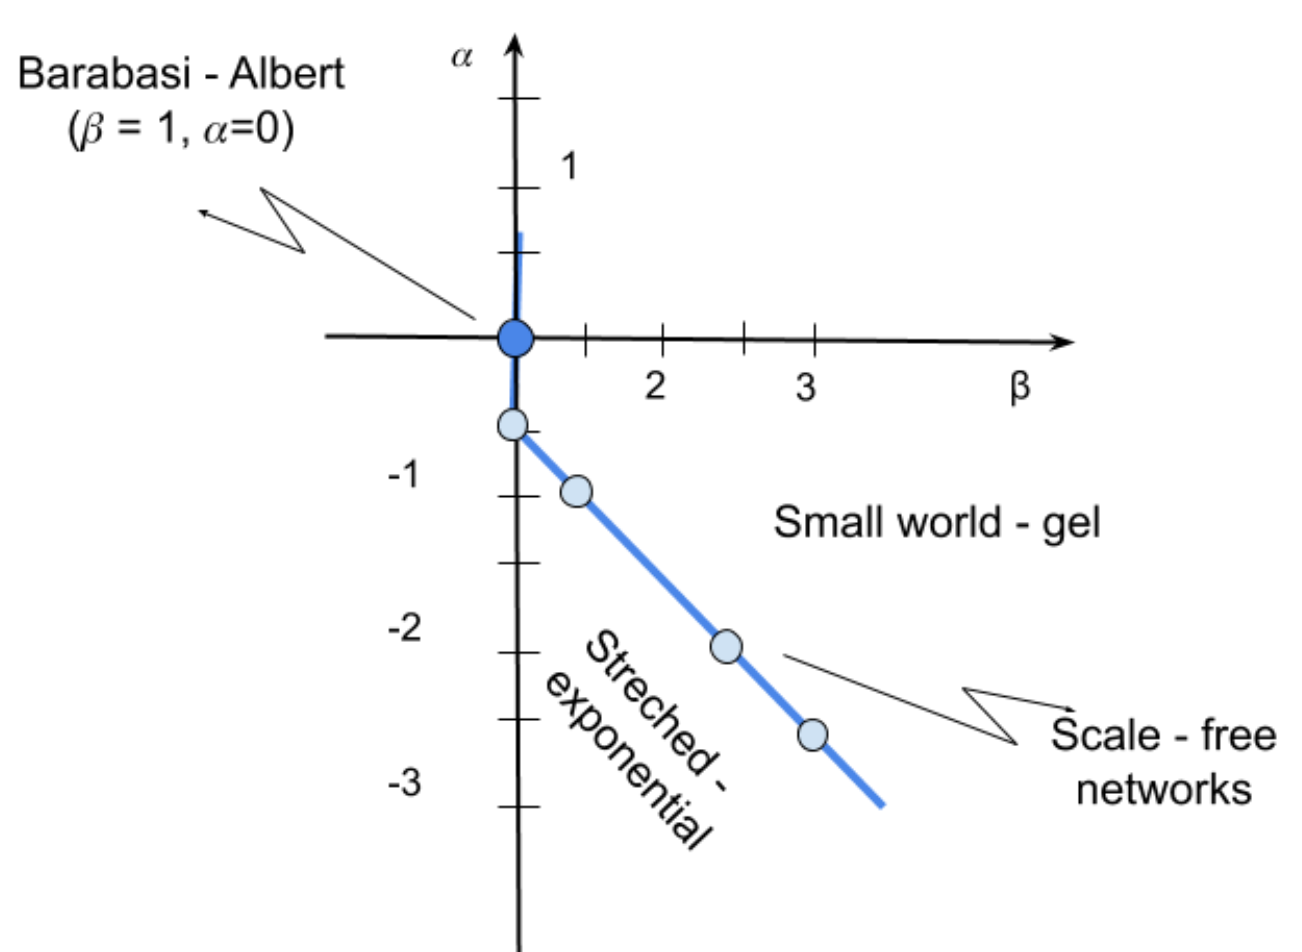
\includegraphics[width=0.6\linewidth]{chapter2/diagram.png}
	\caption[Phase diagram of aging network model]{Phase diagram of aging network model}
	\label{fig:diagram}
\end{figure}

%\newpage

\section{Fractal analysis}

One of the approaches in studying complex systems is detecting the time series of selected variables \cite{kantelhardt2008fractal}. In complex systems, the periodic behaviour of time series is not limited to one or two characteristic frequencies. They extend over a broad spectrum and fluctuations on many time scales and broad distributions \cite{fan2012fractal, sidorov2018fractality}. In these cases, the system's dynamics are characterized by scaling laws, valid over a wide range of time scales or frequencies. When only one scaling exponent describes the system dynamics, the time series is monofractal.
On the other hand, we deal with multifractal time series. Rescaling time $t$ by a factor $a$ may require rescaling the time-series values $x(t)$ by a factor $a^H$; then, we have the self-similarity. The Hurst exponent, $H$, characterizes the type of self-affinity. 
$$x(t) = a^Hx(at)$$. 

\subsection{Long and short-term correlations}
The time series are persistent, meaning that large values usually follow a large value \cite{kantelhardt2008fractal}. Considering the increments $\delta x_i = x_i - x_{i-1}$, of self-affine series $i = 1,.., N$, with N values measured equidistant in time, $\delta x_i$ can be either persistent, independent or anti-persistent. For the random walk with $H=0.5$, the increments are independent. For stationary data with constant mean and standard deviation, the auto-covariance function can determine the degree of persistence. 

\begin{equation}
C(s) = \langle \Delta x_i \Delta x_{i+s} \rangle = \frac{1}{N-s} \sum_{i=1}^{N-s}\Delta x_i \Delta x_{i+s}
\end{equation}


If the data are uncorrelated, the $C(s)=0$. Short-range correlations are described by $C(s)$ declining exponentially
$$C(s) = exp(-s/t_c)$$
such behaviour is typical for increments generated by an auto-regressive process 
$$ \Delta x_i = c\Delta x_{i-1} + \epsilon_i $$
with random uncorrelated offsets $\epsilon_i$ and $c = exp(-1/t_c)$.

For long-range correlations, $\int C(s)$ diverges in the limit for long series. In practice, this means that we can not define the characteristic time because it increases with N. Contrary to short-range correlations, the correlation function decline as power-law 
$$C(s) = s^{-\gamma}$$
Fourier filtering techniques can model this type of behaviour. Long-term correlated behaviour of $\Delta x_i$ leads to self-affine scaling behaviour characterized by Hurst exponent $H=1-\gamma/2$. 

A direct calculation of the $C(s)$ is complex due to present noise in the data and non-stationarity. Non-stationarities make the definition of $C(s)$ problematic because its average is not well defined. Also, $C(s)$ fluctuates around zero on large scales s, so it is impossible to obtain the correct correlation exponent $\gamma$. Instead of calculating $C(s)$, we can calculate the Hurst exponent $H$.

\subsection{Rescaled range analysis} 

Hurst proposed a method called the \textbf{rescaled range analysis} $R/S$, \cite{hurst1951long}. It begins with splitting the time series $x_i$ into non-overlapping segments $\nu$ of the size s, having $N_s = int(N/s)$ segments. Then is calculated the profile in each segment is. 

$$Y_\nu(j) = \sum_{i=1}^{j} (x_{\nu s +i} - \langle x_{\nu s + i } \rangle _s)$$

Substracting the averages, constant trends in the data are eliminated. The differences between minimum and maximum value and the standard deviation in each segment are calculated as $R_{\nu}(s) = max Y_\nu(j) - min Y_{\nu}(j)$, $S_{\nu}(s) = \sqrt{\frac{1}{s}\sum Y^2_{\nu}(j)}$

Finally, the rescaled range is averaged over all segments to obtain the fluctuation function F(s).

$$F_{RS}(s) = \frac{1}{N_s}\sum \frac{R_{\nu}(s)}{S_{\nu}(s)} \sim s^H$$

, where the H is the Hurst exponent. Values $H<1/2$ indicate long-term anti-correlated data while $H>1/2$ long-term positively correlated data \cite{kantelhardt2008fractal}. 

\subsection{Fluctuation analysis}
%%TODO pozvati se na slike

The \textbf{fluctuation analysis} is based on the random walk theory \cite{kantelhardt2008fractal}. For given time series $\{x_i\}$ with length N, we first define the global profile in the form of cumulative sum, equation \ref{eq:cumsum}, where $\langle x\rangle $ represents the average of the time series. 

\begin{equation}
Y(j) = \sum_{i=0} ^j (x_i - \langle x\rangle), \quad j=1, ..., N
\label{eq:cumsum}
\end{equation}
Figure \ref{fig:hurst_signals} shows examples of multifractal, monofractal and white noise signal with their global profiles.

\begin{figure}[h]
	\centering
	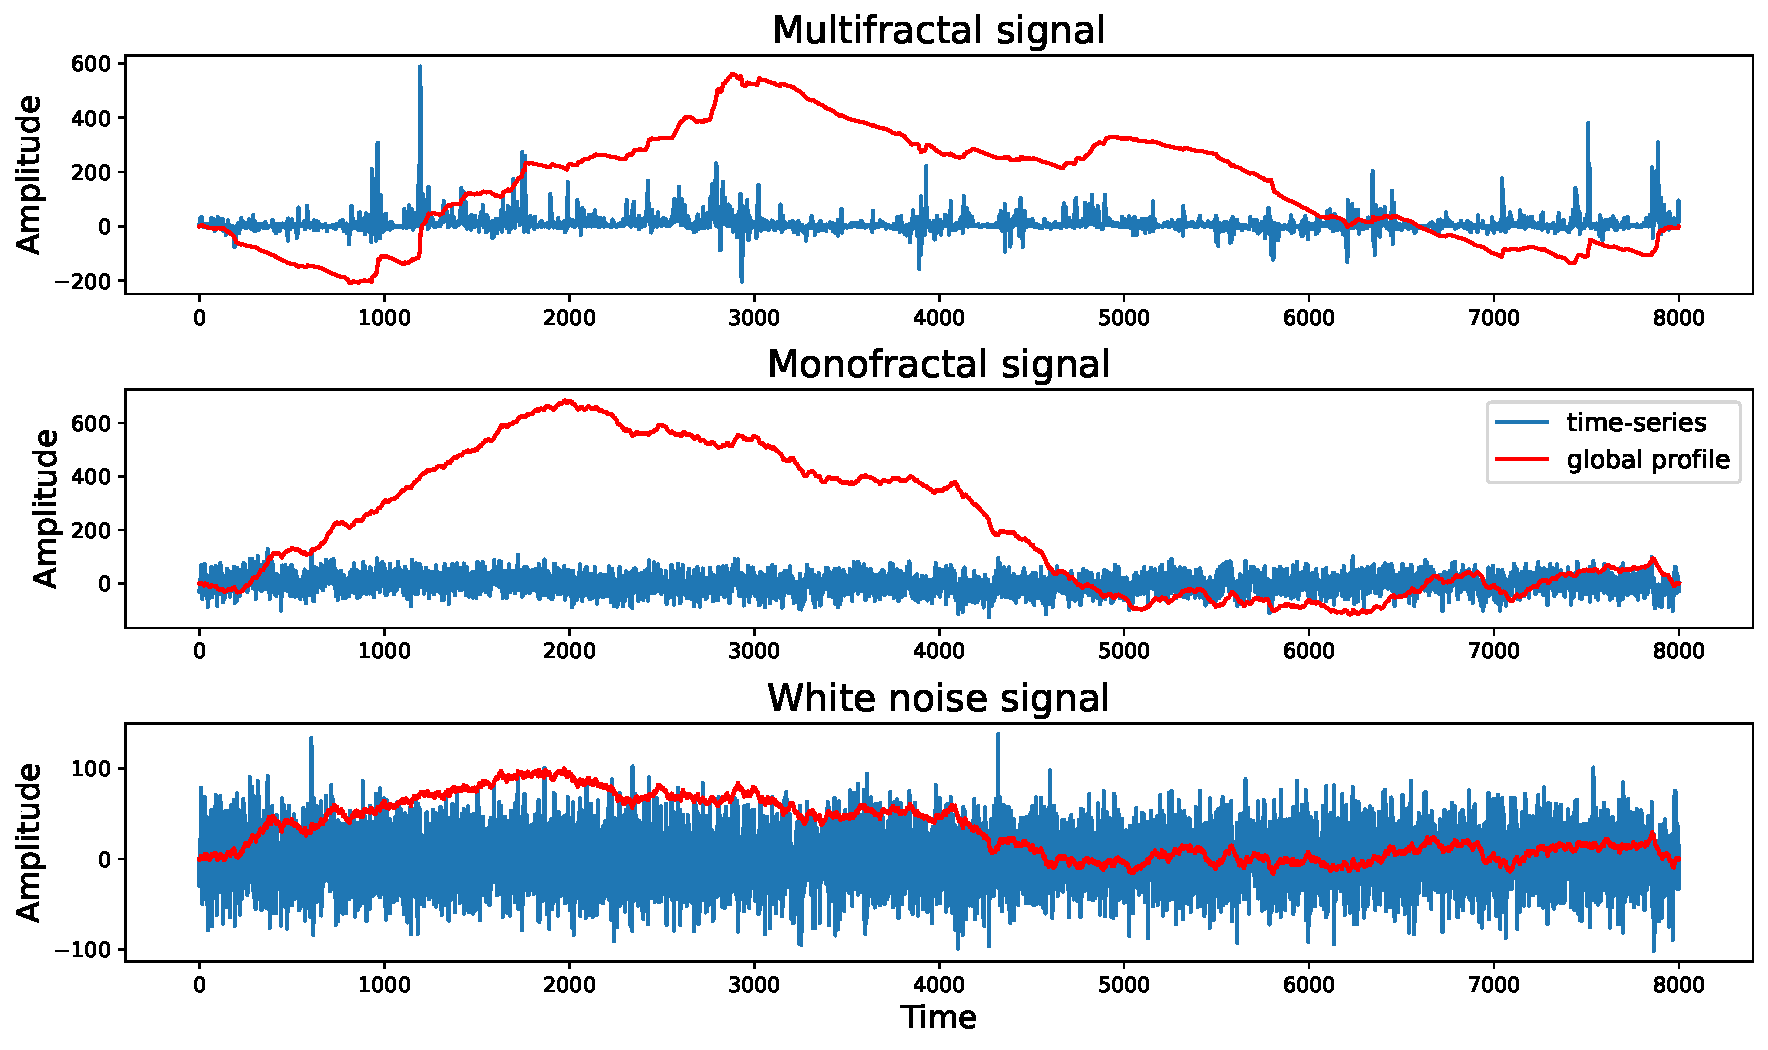
\includegraphics[width=0.8\textwidth]{chapter2/hurst_signals.pdf}
	\caption{Multifractal, monofractal and white noise signals.}
	\label{fig:hurst_signals}
\end{figure}

The profile of the signal Y is divided into $N_s = int (N/s)$ non-overlapping segments of length $s$. The last segment will be shorter if $N$ is not divisible with $s$. That is handled by doing the same division from the opposite side of the time series, giving us $2N_s$ segments. Then we calculate the fluctuations in each segment $F^2(\nu, s)$ and, finally, average overall subsequences, obtaining the mean fluctuation. From the scaling of the function, we can determine the Hurst exponent. 

\begin{equation}
F_2(s) = [\frac{1}{2N_s} \sum F^2(\nu,s)]^{1/2}  \sim s^H
\end{equation} 

Several methods are proposed for calculating the fluctuating function $F^2(\nu, s)$:
\begin{itemize}
	\item {The most straightforward way to calculate the fluctuations is to consider the difference in the values at the endpoints of each segment. It is the same as eliminating the linear trend from each segment.  
	$$ F^2(\nu, s) = [Y(\nu s) - Y((\nu +1)s)]^2$$ 
    Figure \ref{fig:hurst_detrending} shows the global profile of the multifractal signal, divided in segments of the length $s=1000$. On the top panel, each segment $s$ is approximated with linear function.
 }
	
	\item The trends present in the time series do not have to be linear \cite{hu2001effect}. The middle and bottom panel in Figure \ref{fig:hurst_detrending} show that the segments of the signal could be very well approximated with some higher order functions: quadratic or cubic. In general, using the detrended fluctuation analysis (DFA) we could remove the polynomial trend of the order $m$ \cite{kantelhardt2001detecting}.  
	% or any polynomial of order $m$. %When dealing with non-stationary time series, removing the polynomial trend within each segment is necessary by least-square fitting. 
	%The method where polynomial trend is removed is called detrended fluctuation analysis (DFA) .
	From each segment $\nu$, local trend $p^m_{\nu, s}$ - polynomial of order m - should be eliminated, and the variance $F^2(\nu, s)$ of a detrended signal is calculated as in equation:
	
	\begin{equation}
	F^2(\nu, s) = \frac{1}{s}\sum_{j=1}^s \left[Y(j) - p^m_{\nu, s}(j)\right]^2
	\label{eq:var}
	\end{equation}
\end{itemize}
\begin{figure}[h]
	\centering
	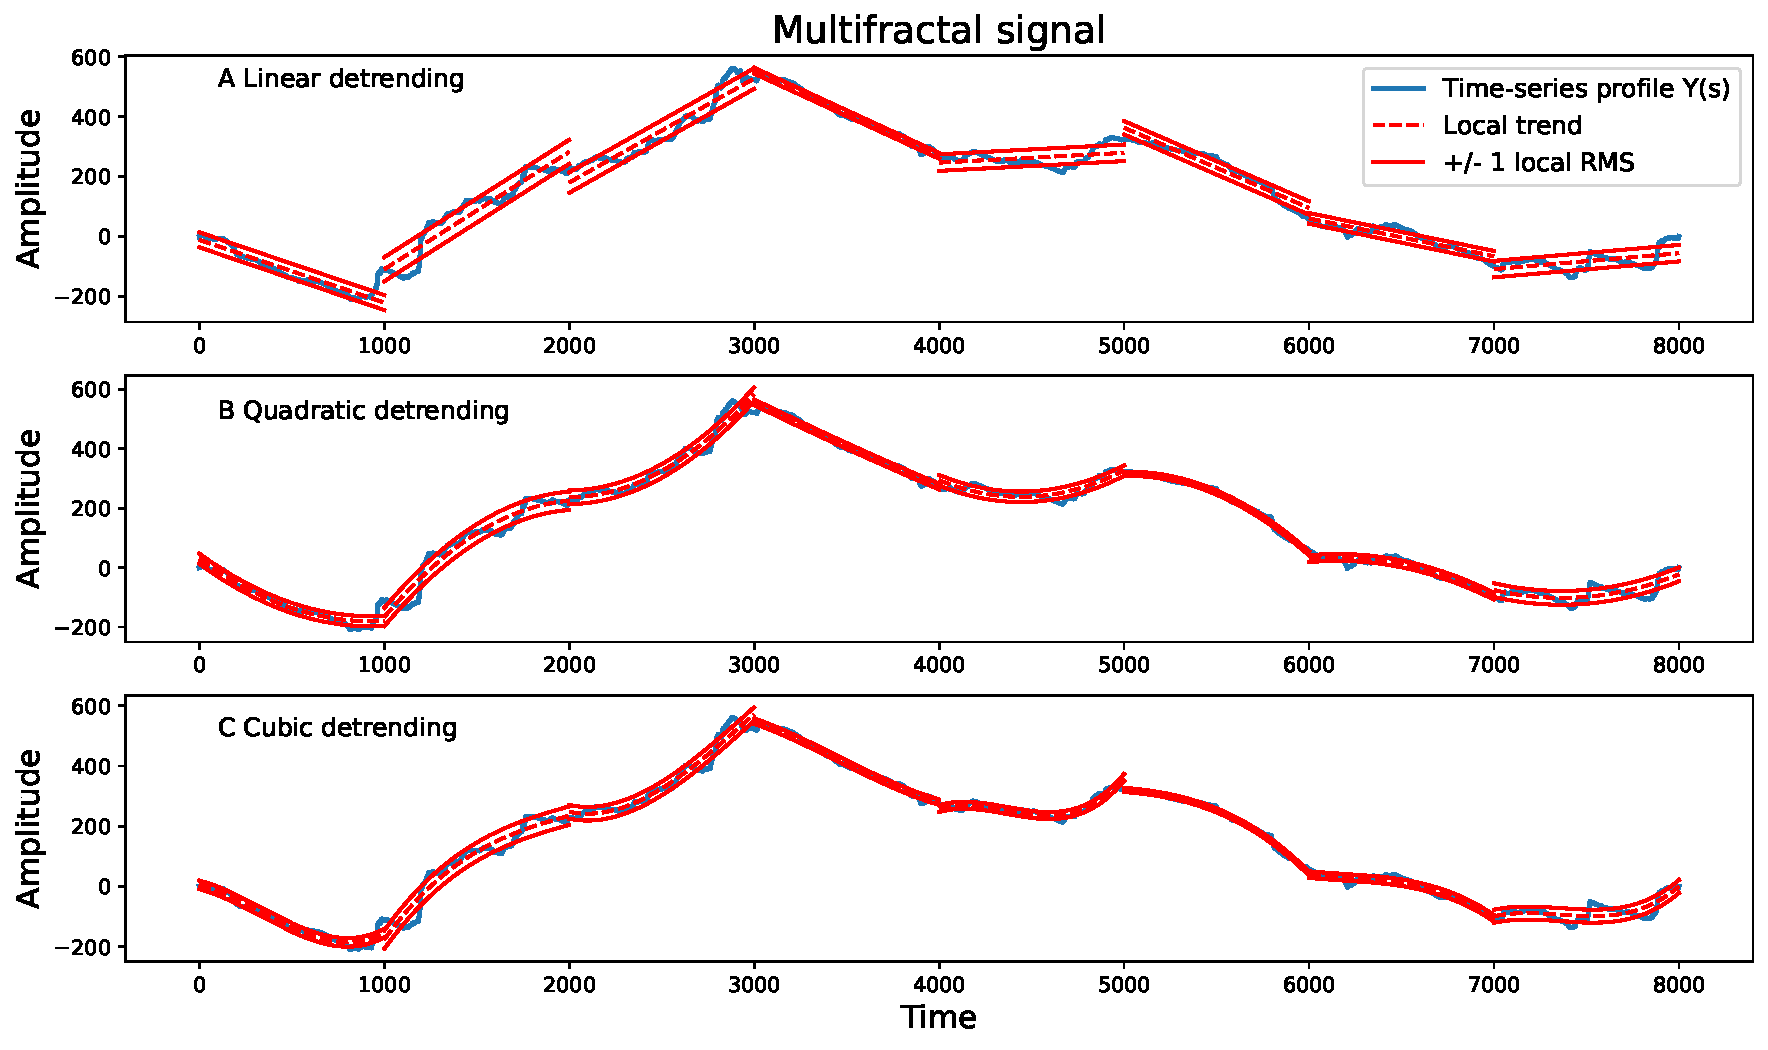
\includegraphics[width=0.8\textwidth]{chapter2/hurst_detrending.pdf}
	\caption{Detrending the signal for the segments of length $s=1000$.}
	\label{fig:hurst_detrending}
\end{figure}


\subsection{Multifractality of the signals}

The scaling behaviour in many data may be more complicated, and different scaling exponents can be found for many interwoven subsets of the time series, representing multifractal. The multifractality may come from the broad probability distribution of the time series values. In this case, the multifractal properties can not be destroyed with shuffling time series. The source of multifractality may be from different small and large fluctuations correlations. In this case, the probability density function of the values can be regular distribution with finite moments, and the corresponding shuffled series will exhibit non-multifractal scaling as correlations are destroyed with the shuffling procedure. When both kinds of multifractality are present, the shuffled time series will show weaker multifractality. 

The multifractal analysis will reveal higher-order correlations. Multifractal scaling can be observed if the scaling behaviour of small and large fluctuations is different. Multifractal detrended fluctuation analysis (MFDFA) is used \cite{kantelhardt2002, ihlen2012} to estimate multifractal Hurst exponent H(q). 

\begin{equation}
F_q(s) = \left\{\frac{1}{2N_s}\sum_{\nu}^{2N_s}\left[F^2(\nu, s)\right]^{\frac{q}{2}}\right\}^{\frac{1}{q}},  q \neq 0 \nonumber
\end{equation}

The MFDFA for $q=2$ is equivalent to the DFA method. The value of $H(0)$, which corresponds to the limit $H(q), q-0$, cannot be determined directly because the exponent diverges. Instead, the logarithmic averaging procedure has to be considered. 
\begin{equation}
F_0(s) = \exp \left\{\frac{1}{4N_s}\sum_{\nu}^{2N_s}ln \left[F^2(\nu, s)\right]\right\}, q=0
\end{equation}

The fluctuating function scales as power-law $F_q(s) \sim s^{H(q)}$ and the analysis of log-log plots $F_q(s)$ gives us an estimate of multifractal Hurst exponent $H(q)$, see Figure \ref{fig:hurst_mfdfa}

\begin{figure}[h]
	\centering
	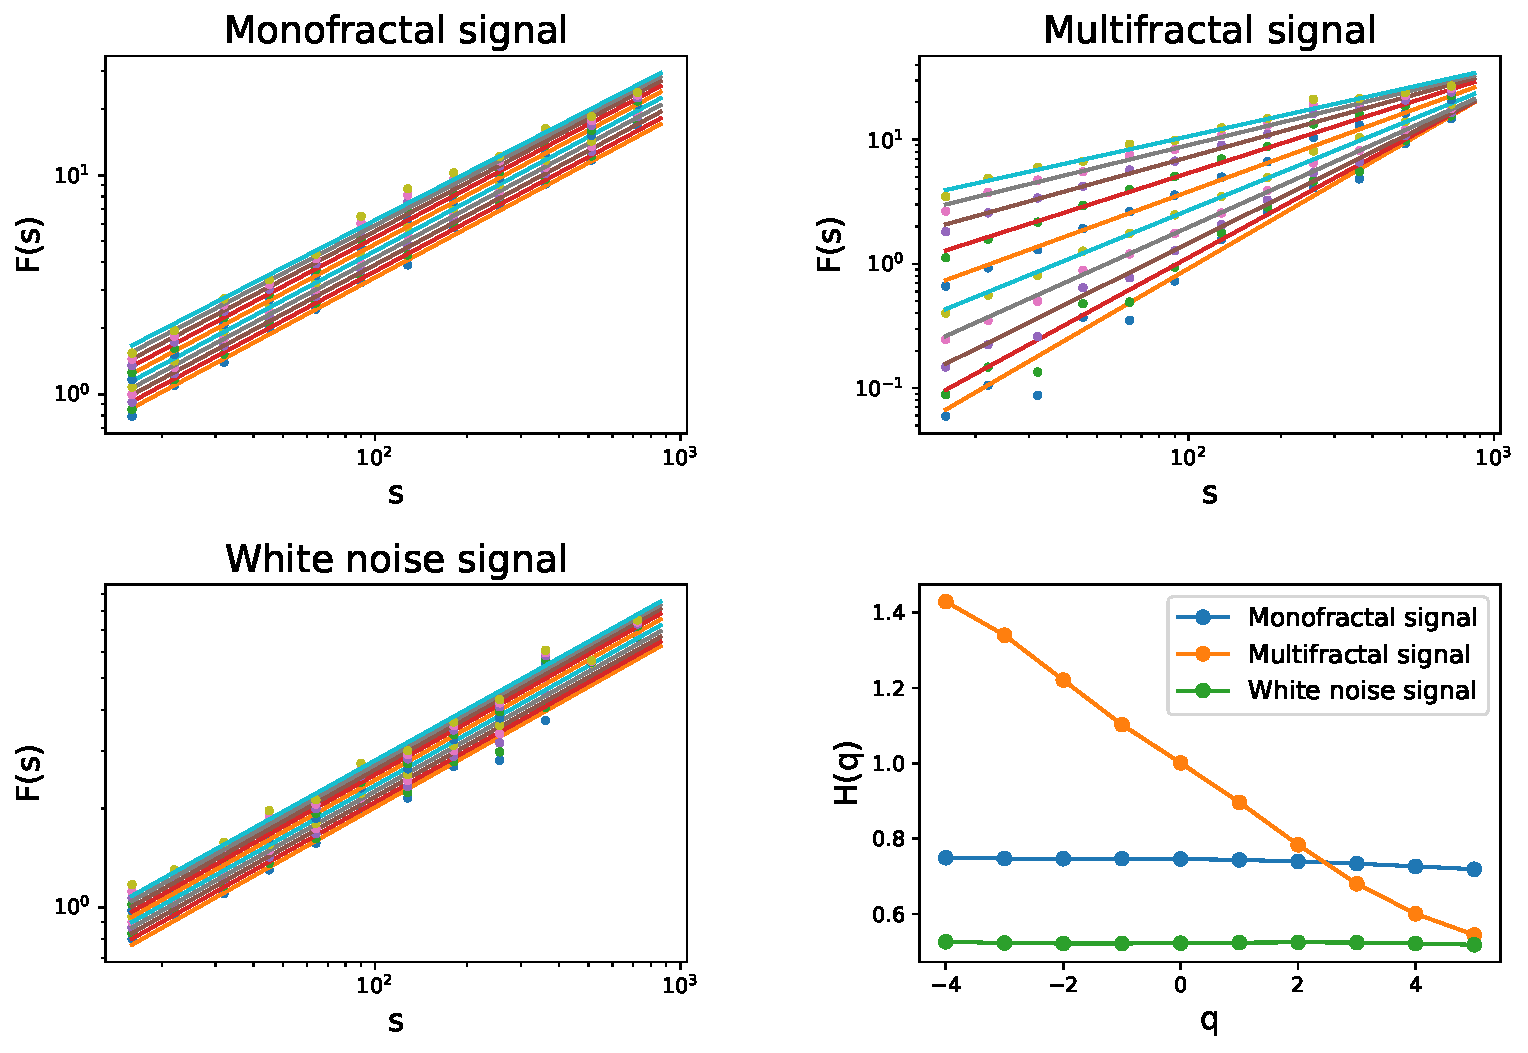
\includegraphics[width=0.8\textwidth]{chapter2/hurst_mfdfa.pdf}
	\caption[Fluctuating function and Hurst exponent.]{Dependence of the fluctuating functions on the scale for monofractal, multifractal and white noise signals, and the dependence of the Hurst exponent $H$ on the scale 1 $q$ for different types of signal (bottom right).}
	\label{fig:hurst_mfdfa}
\end{figure}

For the monofractal time series, H(q) is independent of q, meaning that scaling is identical for all segments, and averaging fluctuations gives identical scaling for all values of q. If small and large changes scale differently, h(q) will depend on q. Positive values of q, segments with large variance are dominant in the Fq(s), so positive q describes segments with large fluctuations. The negative values of q, H(q) describe the scaling of the segments with small fluctuations. 
%Also, large fluctuations are characterized by smaller scaling exponent. 

\section{Dynamical reputation model} \label{sec:met_dibrm}
%%TODO Ok je da odredjivanje parametara bude u apednix-u ali to moras da kazes u samoj sekciji. Ja bih razmislila da moza odredjivanje parametara ne bude u apendixu nego ovde. I to je opcija.

Consider a system where each component has an activity pattern that could be mapped to the discrete signal, representing the moments when the event happened, such as the activity pattern when users are sending an email or communicating, sharing opinions and information within the community. Users' behaviour directly influences their position in the community, which is measured through reputation. The trust among users depends on the amount of interaction between them, which means the trust changes over time. The computational model needs to capture the dynamic property of the trust. Furthermore, the important property of the trust is that it is easier lost than gained; the frequency of interaction also matters. The trust between users who interact frequently should increase faster than between users who rarely interact. 

With Dynamic Interaction Based Reputation Model (DIBRM) \cite{melnikov2018toward}, we can quantify the user reputation $R_n$ after each interaction using equation \ref{eq:tn}, where $n$ is the number of interaction $n\in{1, N}$.
\begin{equation}\label{eq:tn}
R_{n}=R_{n-1} \beta^{\Delta_{n}} + I_{n}
\end{equation}

The first part of the equation considers the reputation value after the previous interaction $R_{n-1}$, weighted with coefficient $\beta^\Delta_{n}$. Depending on the frequency of the interaction, reputation will rise or decay. Parameter $\beta$ ranges from $0<\beta < 1$ is forgetting factor. The $\Delta_n$ measures time between two interactions $t_n$ and $t_{n-1}$: 
\begin{equation}\label{eq:deltan}
\Delta_{n}=\frac{t_{n}-t_{n-1}}{t_{a}}
\end{equation}
where $t_a$ is the characteristic time window of interaction. In the second part of the equation, $I_n$ is the reputation gained within each interaction. The basic value of each interaction is given as $I_{bn}$, and the parameter $\alpha$ is the weight of the cumulative part. 
\begin{equation}\label{eq:ibn}
I_n  = I_{b_{n}}(1 +  \alpha  (1-\frac{1}{A_n+1}))
\end{equation}

When $\Delta_{n}<1$, a user is frequently active, meaning that the time between two interactions is less than the characteristic time window. The number of sequential activities $A_n$ increases by 1. On the other hand, when $\Delta_n>1$ is large, the reputation decays, while the number of activities resets to $A_n=1$. 

\begin{figure}[h]
	\centering
	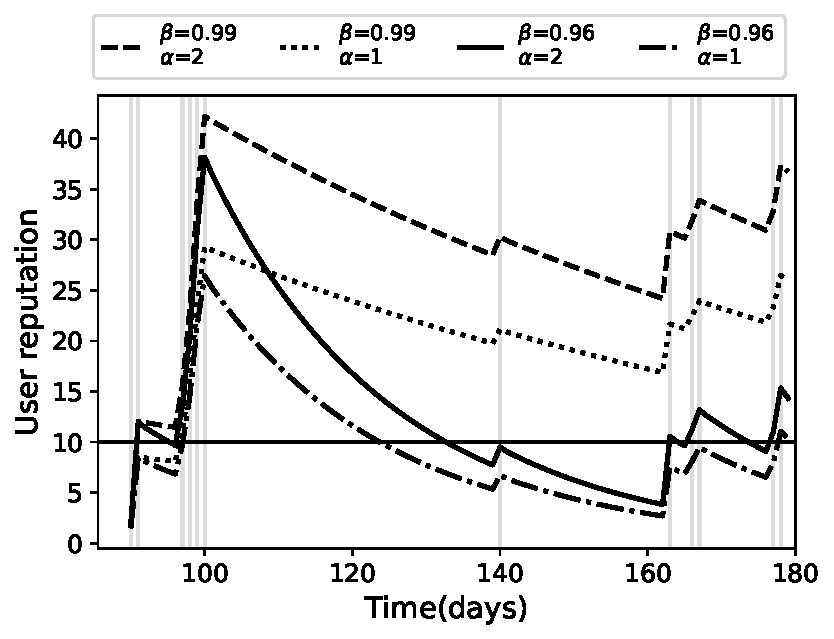
\includegraphics[width=0.45\textwidth]{chapter2/DIBRM.pdf}
	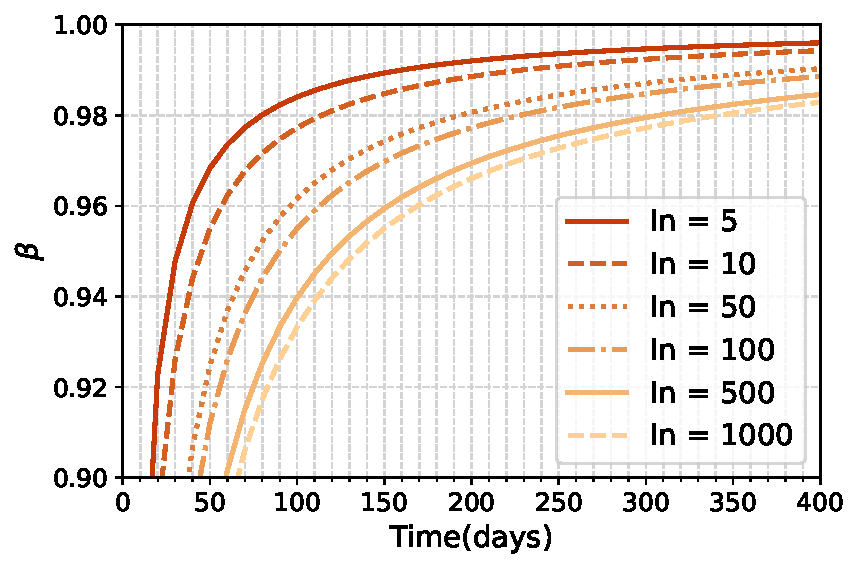
\includegraphics[width=0.45\textwidth]{chapter2/DIBRM_decay.pdf}
	\caption{User reputation.}
	\label{fig:reputation}
\end{figure}  

For example, if we set the characteristic window size and basic value of interaction to $t_a=1 day$, $I_{bn}=1$, we can analyze the influence of the parameters $\alpha$ and $\beta$ on the user reputation. Lower $\alpha$ and $\beta$ values lead to faster reputation decline, as shown in Figure \ref{fig:reputation} - left panel. With lower $\beta$, the reputation may quickly drop close to the reputation threshold, under which we don't consider the user as active. In contrast, with larger values of $\beta$, reputation stays high even if a user is inactive for a larger period. The parameter $\alpha$ is the most important influence on burst behaviour, where larger $\alpha$ leads to higher reputation values. 

If a user is frequently active, we can record the reputation after each day. On the other hand, if $t_n-t_{n-1}>1 \text{day}$ we need to interpolate the reputation values for each day between two interactions, $t_{n-1}<t_d<t_{n}$. To do that, we consider that due to inactivity, reputation will only decay, so it could be calculated as $R_d = R_{n-1}\beta^{\Delta_d}$, where $\Delta_d=(t_{d}-t_{n-1})/t_a$. 

When a user becomes inactive, its reputation starts to decline, and when it drops below the reputation threshold user does not have any influence on the community. We can approximate the dependence of parameter $\beta$ and time $\delta t$ needed for reputation to reach this level as $\beta = (\frac{R_0}{R_i})^{\frac{t_a}{\delta t}}$. In the examples in Figure \ref{fig:reputation}, - right panel, the parameter $t_a=1\text{day}$, while we vary different starting reputation levels $I_n$.   
For $\beta$ values below $0.96$, the decay is fast, and within two to four months of inactivity, even high reputation values are
reduced below the threshold. On the other hand, with values of $\beta$, the decay process is more differentiated, and the high
reputation becomes harder to lose, surviving up to a year of inactivity. For $\beta$ equal to $0.96$, reputation with starting value $5$ needs around one month to decay below the threshold. For higher reputations, $500$ or $1000$, the decay period is around $5$ months. 

In this model, the user's reputation changes continuously through time, decreases when the user is inactive and grows with frequent and constant user contribution. The highest growth of a user's reputation is found through bursts of activity followed by a short period of inactivity. With model parameters, $I_{bn}, t_a, \alpha, \beta$, the dynamic of user reputation may be controlled and adapted to different communities. If the community has its reputation system, we can also fit the model parameters to mimic the actual reputation dynamic. In this thesis DIBRM model is used to analyse Stack Exchange communities, Chapter \ref{Ch:Trust}, while in Appendix \ref{App:parameters} we suggest procedure to estimate the model parameters for this specific system. 
















%% Chapter 1

\chapter{Driving signals} % Main chapter title
\label{Ch:signals} % For referencing the chapter elsewhere, use \ref{Chapter1} 

The complex networks grow by adding new nodes, and growing network models consider growth constant over time. This approximation is sufficient for explaining how properties of complex networks can emerge; for example, we find scaling of degree distribution in the Barabasi-Albert model, such as in real systems. Models mainly focus on linking rules and their influence on the topology of complex networks. 

Still, the growth of real systems changes over time. In online social networks, new users join daily, and the users' activity might have bursty nature. We can consider a co-authorship network, where links are created between scientists when they publish a paper. The dynamic of real networks can be complex and highly influenced by non-linear signals. The growth signal, the number of new nodes in each time step, has cycles and trends. Circadian cycles are directly reflected in growth signals, and we also find long-range correlations and multifractal properties. 

In this chapter, we explain the properties of growth signals, both real and computer-generated. We analyze networks created with a growing network model where the interplay between ageing and preferential attachment shapes their structure. We are interested in incorporating non-constant growth signals into the model and measuring their impact on the complex networks. Differences between networks with the same number of nodes and links can be observed by analyzing connectivity patterns. Figure \ref{fig:ciljevi} describes our goals. 

\begin{figure}[!ht]
	\centering
	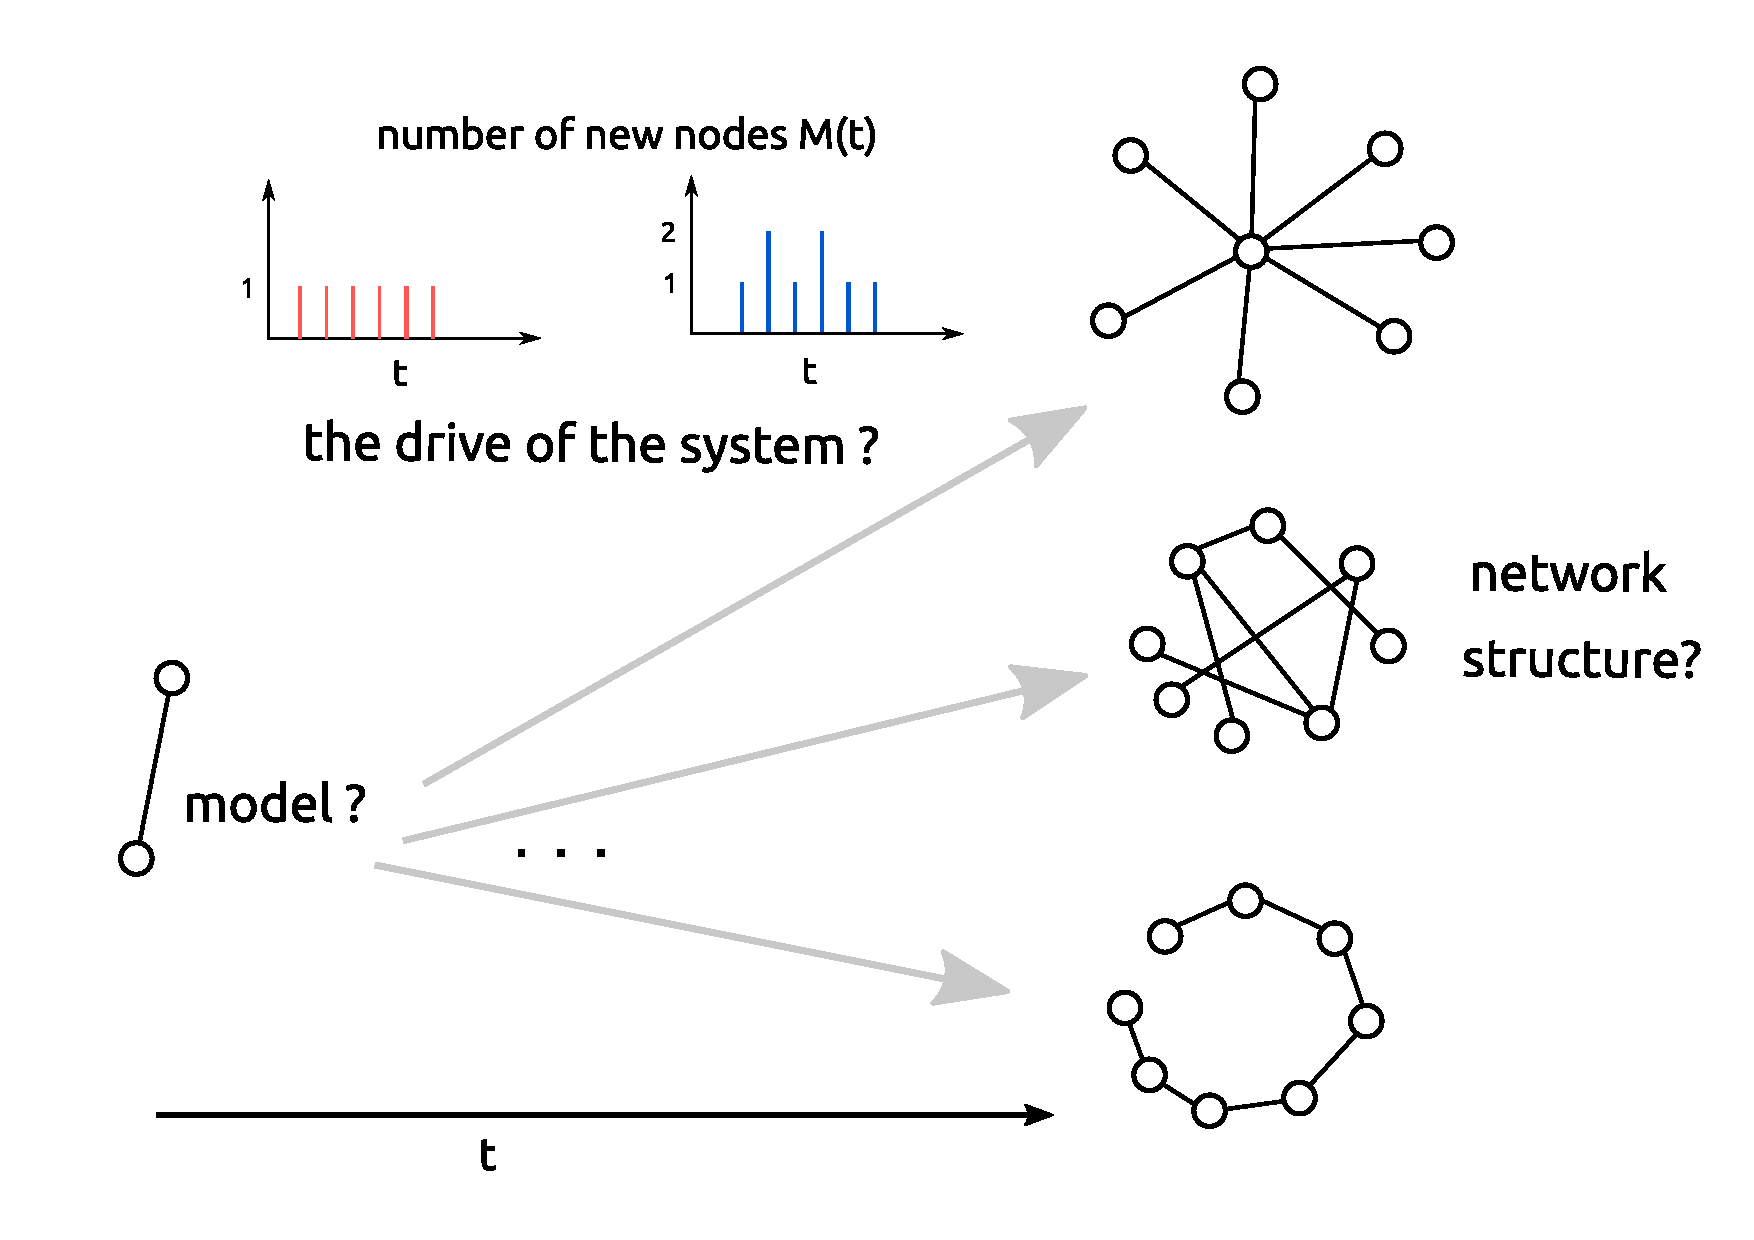
\includegraphics[width=0.7\linewidth]{ciljevi.pdf}
	\caption[Nonlinear growth of network.]{The open question is how nonlinear signals in combination with network model influence the structure of the network. Under what circumstances networks have the scale-free, hub-spoke or chain structure. }
	\label{fig:ciljevi}
\end{figure}

\section{Aging network model with growth signal}

To enable nonlinear network growth in the number of nodes, we need to adapt the existing models such that at each time step, we can add $M\geq1$ new nodes that make $L\geq1$ links with existing nodes in the network. The master equation $N_k$, $k$ degree nodes can be written as: 

\begin{equation}
\partial_{t}N_{k}=\sum^{M(t)}_{j=1}r_{k-j\longrightarrow k}N_{k-j}-\sum^{M(t)}_{j=1}r_{k\longrightarrow k+j}N_{k}+M(t)\delta_{k,L} . \label{eq:aging_master}  
\end{equation}

At each time step we add $M(t)$ nodes with $L$ links. As multiply links between two nodes are not allowed, we'll get $M(t)$ new nodes with degree $L$, which describes the third term in the equation. Old nodes can increase their degree from 1 to $M(t)$, as different new nodes can choose the same node. The first term in the equation describes nodes with degree $k\in\{k-M(t),\ldots, k-1\}$ that getting degree $k$, while in second term nodes with degree $k$ entering degree  $k\in\{k+1,\ldots, k+M(t)\}$. The quantities $r_{k-j\longrightarrow k}$ and $r_{k\longrightarrow k+j}$ are the rates that express the transitions of a node from class with degree $k-j$ to one with degree $k$ and from class with degree $k$ to class with degree $k+j$ respectively.  

For model we choose, aging model where linking probability depends on network degree $k$ and its age $\tau$, $\Pi_{i}(t)\sim k_{i}(t)^{\beta}\tau_{i}^{\alpha}$. With this linking probability the master equation was solved for $M(t)=const.=1$, using  approach \cite{dorogovtsev2001b}. When $M(t)$ is the correlated function, the equation is not solvable analytically. Instead, we use numerical simulations to study the influence of the signal $M(t)$ on the network structure. When we add only one link per node $L=1$, networks are uncorrelated trees. To obtain the clustered structures, we need to use $L>1$; so each new node can create more than one link. Finally we focus on the aging model parameters $-\infty<\alpha\leq-1$ and $\beta\geq1$. We expect critical line $\beta(\alpha^{*})$ where scale-free networks can be found. Under critical line, networks have stretched exponential degree distribution, and for large $\beta$ small-world networks are present. 

Finally, we need to define what the time series of new nodes are. We focus on the growth of two real systems, the \textbf{TECH} \cite{smiljanic2017associative} community in the Meetup website and on two months of \textbf{MySpace} \cite{suvakov2013} social network. 

\subsection{Time-series from real systems}

MySpace signal is the number of new members who appear for the first time in the data. The dynamics of the Meetup website happen on different scales than on Meetup. Here, the time step is one minute. The MySpace signal has $T = 3162$ steps, with  $N = 10000$ members.  To describe the properties of the signal, we use Multifractal detrended analysis and calculate the Hurst exponent on different scales, showing the right pane of the figure, \ref{fig:myspace_signals}. It is multifractal $q<0$, and becomes constant for $q>0$, it has long-range correlations as $H(q=2)=0.6$. My Space signal has cycles characteristic of the human circadian rhythm, figure $\ref{fig:myspace_signals}$. If we randomize the MySpace signal, we find that we can easily destroy trends and cycles. The randomization is done with the reshuffling procedure, where we keep number where we keep the number of nodes, length and the mean value of the signal. The inset of the original and randomized signals show the time series' global profile; we find that trends are destroyed. Also, randomized MySpace signal does not have long-range correlations anymore, Hurst exponent indicates short-range correlations $H=0.5$, and the signal becomes monofractal.    


\begin{figure}[H]
	\centering
	\begin{minipage}[b]{0.4\textwidth}
		\centering
		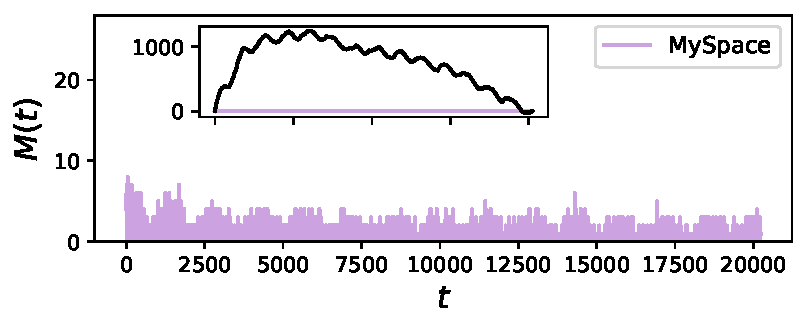
\includegraphics[width=\textwidth]{signal4.pdf}\\
		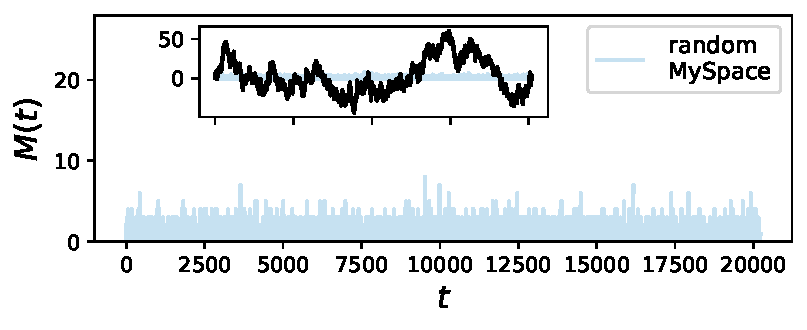
\includegraphics[width=\textwidth]{signal5.pdf}
	\end{minipage}
	\begin{minipage}[b]{0.45\textwidth}
		\centering
		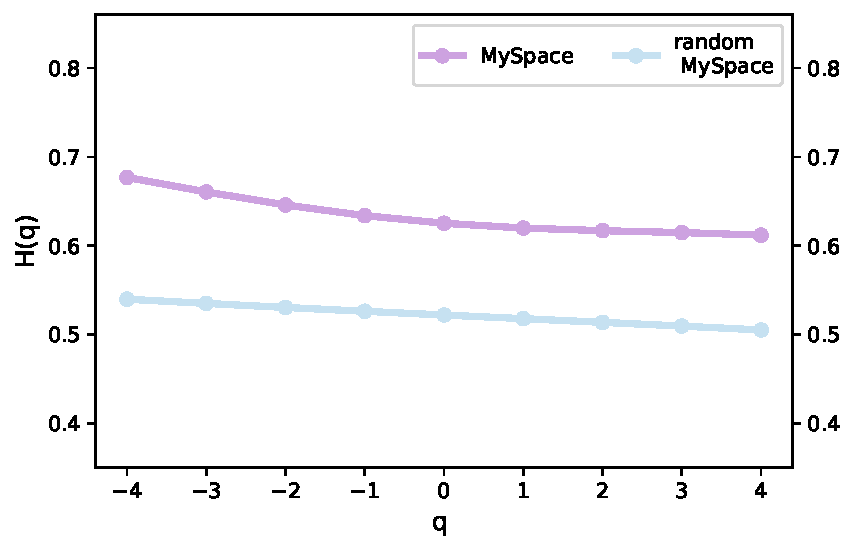
\includegraphics[width=\textwidth]{hurst_myspace.pdf}
		\vspace{0.01cm}
	\end{minipage}
	\caption[Properties of MySpace signal.]{MySpace signal, the random MySpace signal (left pane) and the dependence of multi fractal Hurst exponent $H(q)$ of the scale $q$. (right pane)}
	\label{fig:myspace_signals}
\end{figure}

\begin{figure}[ht]
	\centering
	\begin{minipage}[b]{0.4\textwidth}
		\centering
		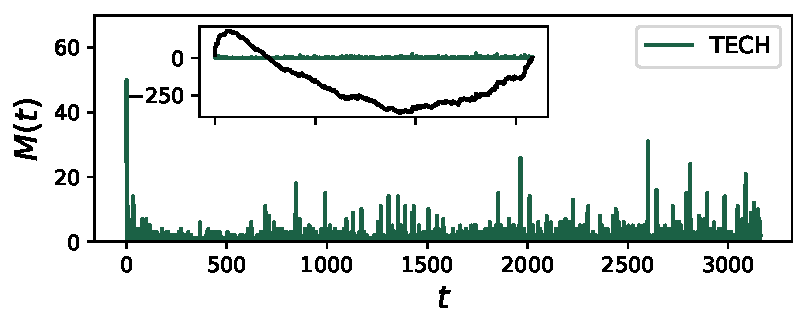
\includegraphics[width=\textwidth]{signal1.pdf}\\
		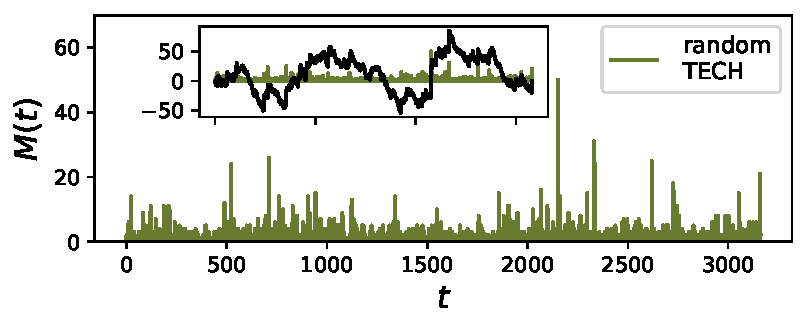
\includegraphics[width=\textwidth]{signal2.pdf}\\
		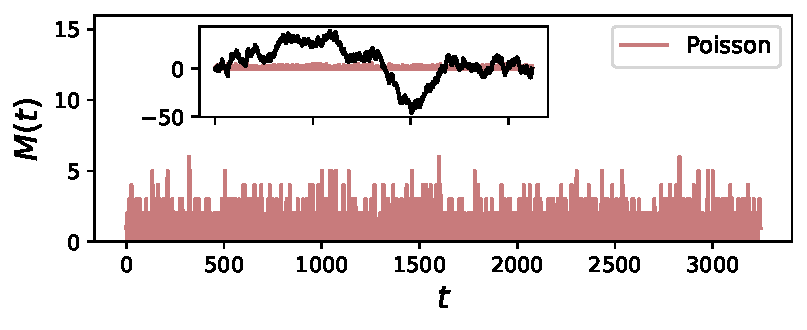
\includegraphics[width=\textwidth]{signal3.pdf}
		
	\end{minipage}
	\begin{minipage}[b]{0.45\textwidth}
		\centering
		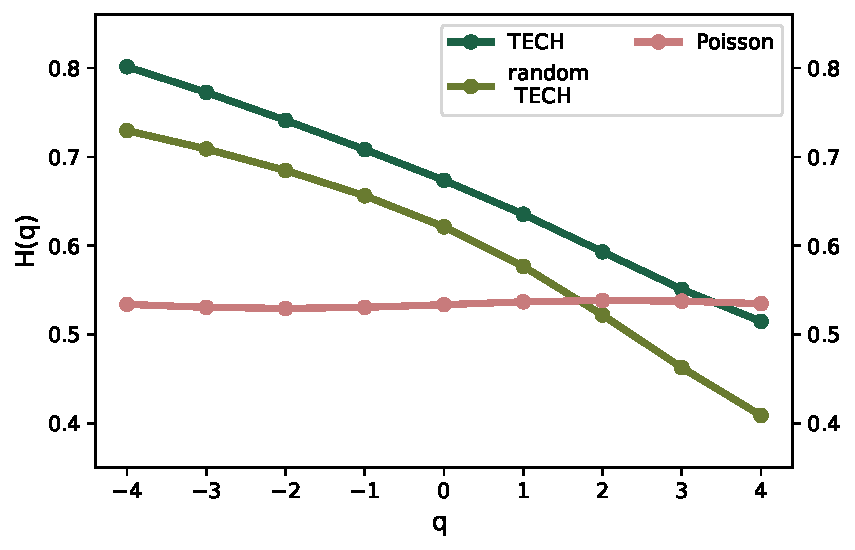
\includegraphics[width=\textwidth]{hurst_tech_1.pdf}
		\vspace{1cm}
	\end{minipage}
	\caption[Properties of the TECH and Poisson signals.]{TECH signal, the random TECH signal (left pane) and the dependence of multi fractal Hurst exponent $H(q)$ of the scale $q$. (right pane)}
	\label{fig:tech_signals}
\end{figure}

The TECH is a group from the Meetup website that gathers users interested in technology. Using the Meetup website, they organize offline events. The time unit in this time series is an event since then are created links between event. The TECH time series M(t) represents the number of users who joined the TECH community and visited the event for the first time. The time series length is $T=3162$ steps, and we count $N=3217$ members in the TECH community for a given period, \ref{fig:tech_signals}. TECH signal has long-range correlations with Hurst exponent $H(q=2)=0.6$. Also, we find that TECH is multifractal, as the Hurst exponent is not constant across the scales. The multifractality originates not only from signal trends but also from the broad probability distribution of time series. If we randomize the TECH signal, we find that we can easily destroy trends and cycles, but signal keeps multifractal properties, meaning that broad probability distribution can not be eliminated. For that reason, we generate the uncorrelated signal from Poissonian probability distribution. The length of this signal is  $T = 3246$, while we keep the number of nodes $N$ same as in TECH signal.


\subsection{D-measure}

We can compare the networks with the same number of nodes and links generated with growth signals with different properties. We use growing network model where we vary parameters $-3<\alpha\leq-1$ and $-3\leq\beta\leq1$. We also vary the network density, $L\in\{1,2,3\}$. For each set of model parameters $\alpha, \beta, L$ and each signal $M(t)$, we create the sample of $100$ networks. Besides this, for the same set of parameters, we generate the sample of networks with $N=10000$ and $N=3217$ nodes grown with constant signal $M(t)=1$; one node is added to the network at each time step. To examine how different growing signals influence the structure of networks, we use D-measure \cite{tiago2}, defined methodology chapter. We equally consider the global and local properties, setting parameter $w=0.5$. We compare the networks grown with the constant and fluctuating signal with D-measure, for all network pairs between two samples, and averaging the result. The advantage this measure has is that it can measure the distance between two network structures, even if they are generated with the same model; that was not the case with Hamming distance or graph editing distance \cite{tiago2}.

Obtained results for D-measure are presented on the figure \ref{fig:dmeasure}. We note that the largest distance between networks is along critical line $\beta(\alpha^{*})$ of the aging model. The fluctuations present in the signal mostly influence, the scale-free networks. For networks, away from this line, structural differences exist, but they are much smaller. For gel small world networks, $\beta>\beta^{*}$, the D-measure is close to zero. Under critical line, $\beta<\beta^{*}$, D-measure depends on the properties of the signal. If we fix network density $L$, position of critical line is independent of the properties of the signal. Still, with higher link density, critical line slightly move toward larger $\beta$, see figure \ref{fig:dmeasure}.

\begin{figure}[ht]
	\centering
	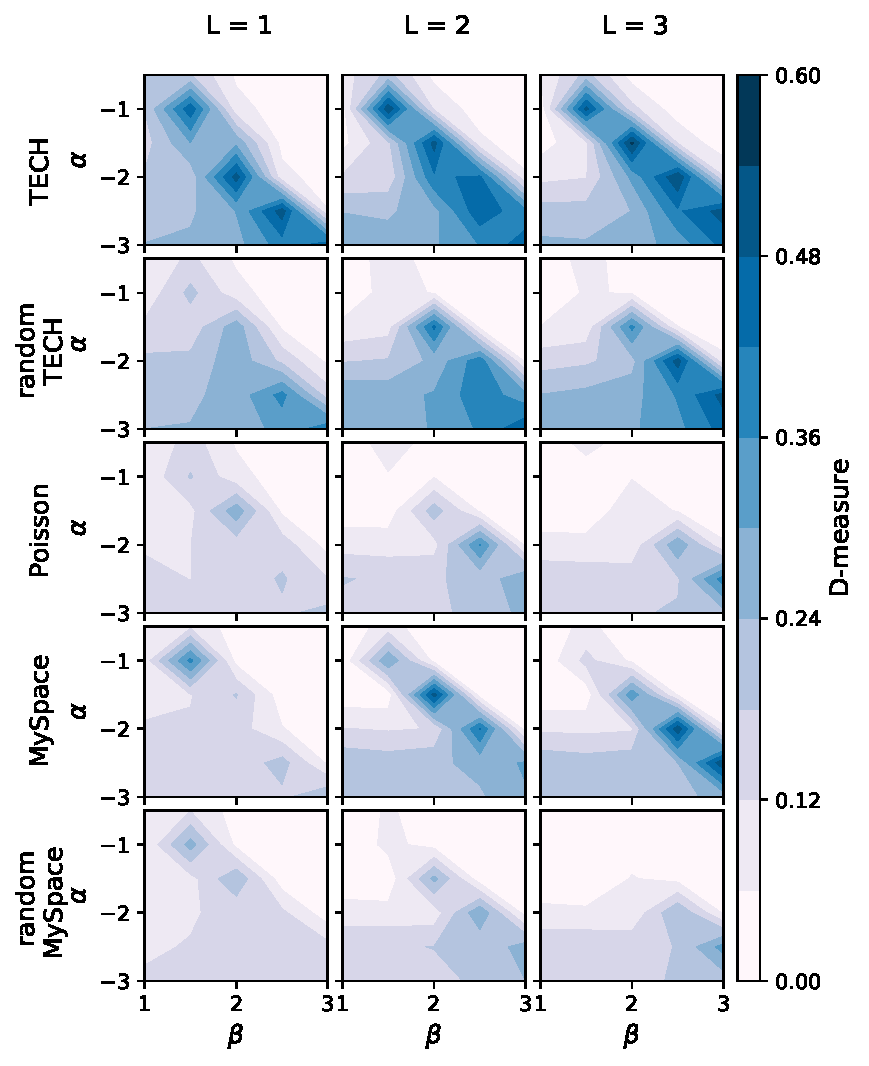
\includegraphics[width=0.6\linewidth]{Ddistance.pdf}
	\caption[D-measure for networks generated with real signals.]{The comparison of networks grown with growth signals shown in figures \ref{fig:tech_signals} and \ref{fig:myspace_signals} versus ones grown with constant signal $M=1$, for value of parameter $\alpha\in[-3,-1]$ and $\beta\in[1,3]$. $M(t)$ is the number of new nodes, and $L$ is the number of links added to the network in each time step. The compared networks are of the same size.}
	\label{fig:dmeasure}
\end{figure}

In the region around the critical line, we find that D-measure depends on the properties of the signal. Multifractal signals TECH has the most considerable impact on network structure; the maximum value of the D-measure is $D_{max}=0.552$. Similar behaviour is discovered for other multifractal signals, random TECH and MySpace. For networks generated with uncorrelated signals: random MySpace and Poisson, difference exists but it is much smaller.

D-measure rises for lower $\alpha$. In the case of a constant signal, the number of nodes added to the network is equal for each time step, so at time interval $T$, the network has $MT$ nodes. In fluctuating signal, the number of nodes added during time interval $T$ vary. In signals, such as TECH, where there are peaks in the number of new users, hubs emerge faster. As we decrease the parameter $\alpha$, fluctuations in the signal become more critical, and the hubs emerge even for uncorrelated signals. The trends in the real signals further promote the emergence of hubs in the network.  

\subsection{The structure of networks}

We examine degree distribution, degree correlations and clustering coefficient of networks generated by real signals. It has been shown that these measures provide a sufficient set for describing the structure of complex networks. Results showed that multifractals influence networks more than monofractals; it is most prominent in scale-free networks. 

Figure \ref{fig:properties_net} shows properties of networks generated with model parameters $L=2$, $\alpha=-1.0$, $\beta=1.5$, that lies on critical line.  The degree distributions $P(k)$ of networks generated with real signals TECH and MySpace have super-hubs emerged. Degree distributions generated with randomized and white noise signals do not differ from the degree distribution of networks generated with the constant signal. Networks generated with real signals average neighbouring degree $\langle k\rangle_{nn}(k)$ and clustering coefficient $c(k)$ depend on node degree, while in networks generated with constant and randomized signals, they weakly depend on the degree $k$.

We also find structural differences between networks, obtained with model parameters under the critical line $\alpha<\alpha^{*}$, see Figure \ref{fig:properties_net}. The difference is mostly found for TECH signal. Degree distribution $P(k)$ shows the emergence of hubs in networks grown with TECH signal, while the randomized and Poisson signals are more similar to networks grown with the constant signal. MySpace signal, whose generalized Hurst exponent $H(q)$ weakly depends on scale parameter $q$ and whose long-range correlations and trends are easily destroyed, do not influence the structure of networks more than constant or randomized signal.   

The properties of the time-varying signal do not influence the topological properties of small-world gel networks, Figure \ref{fig:properties_net}. Here model promotes the existence of hubs. As this is the mechanism through which the fluctuations alter the structure of evolving networks, the properties of the signal are not relevant.   

\begin{figure}[H]
	\centering
	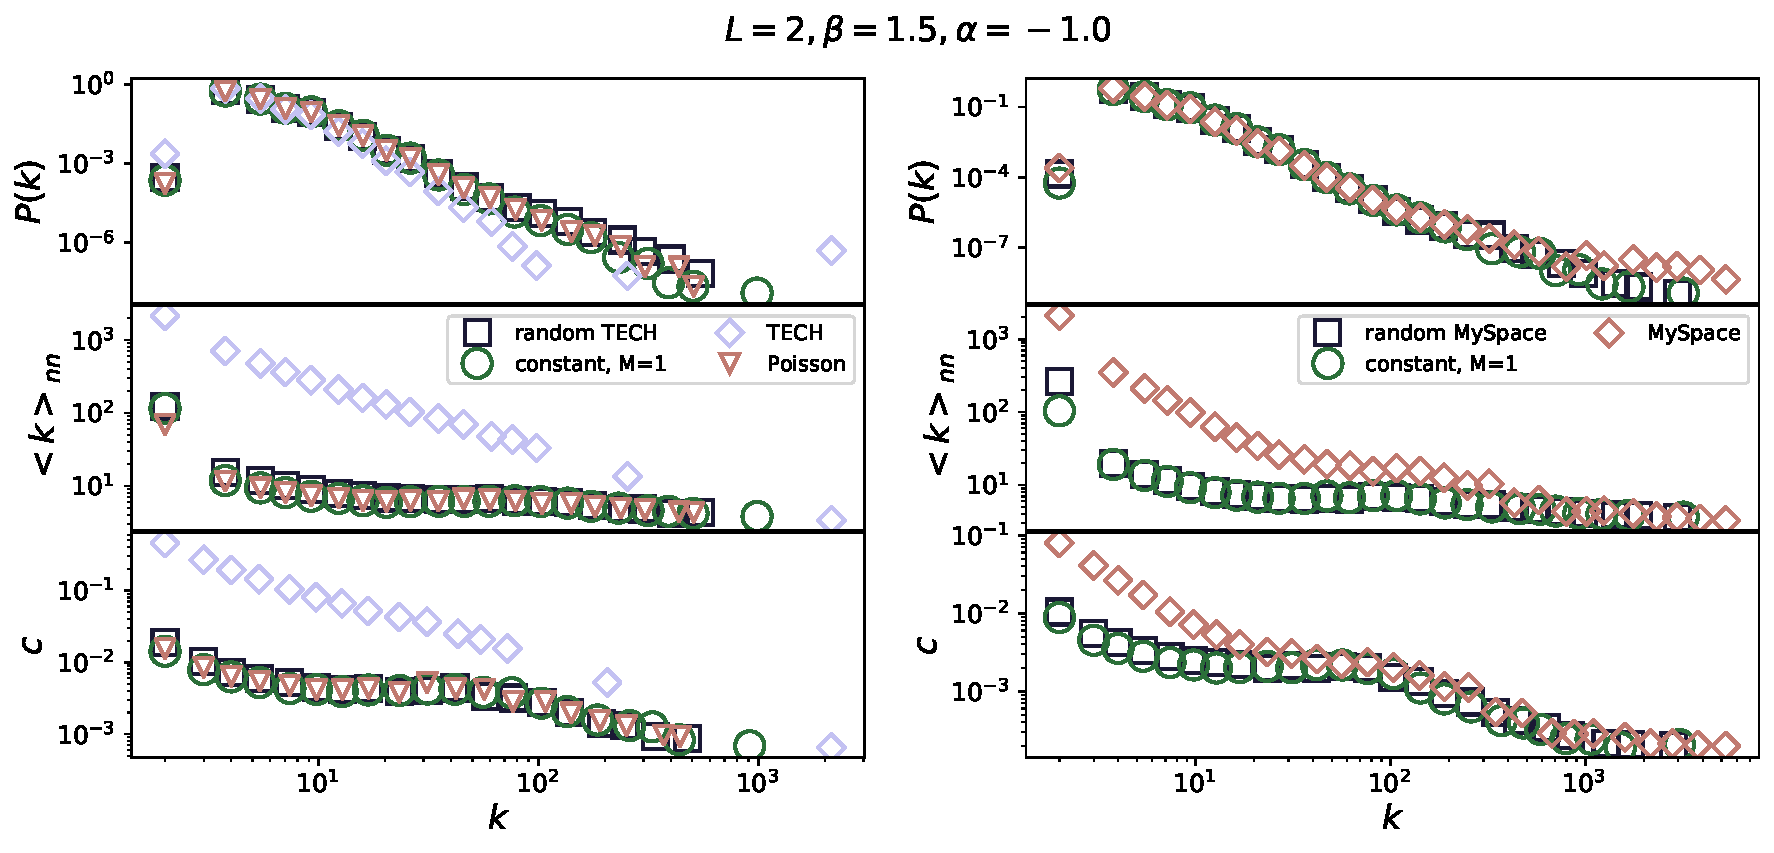
\includegraphics[width=0.9\textwidth]{b1.pdf}
	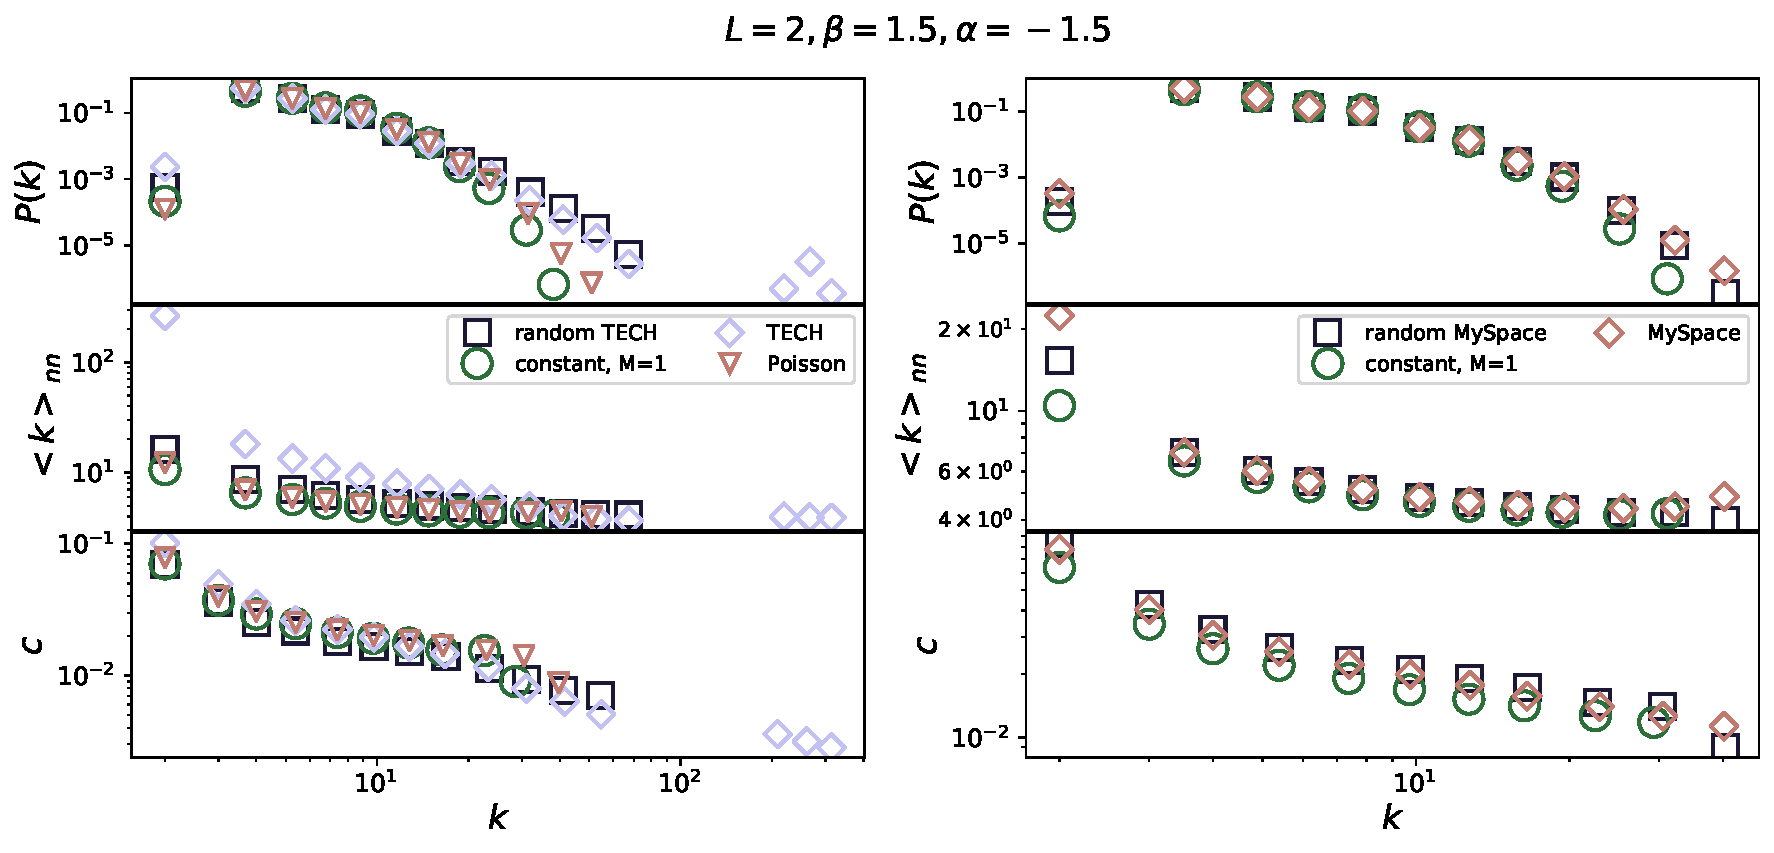
\includegraphics[width=0.9\textwidth]{b3.pdf}
	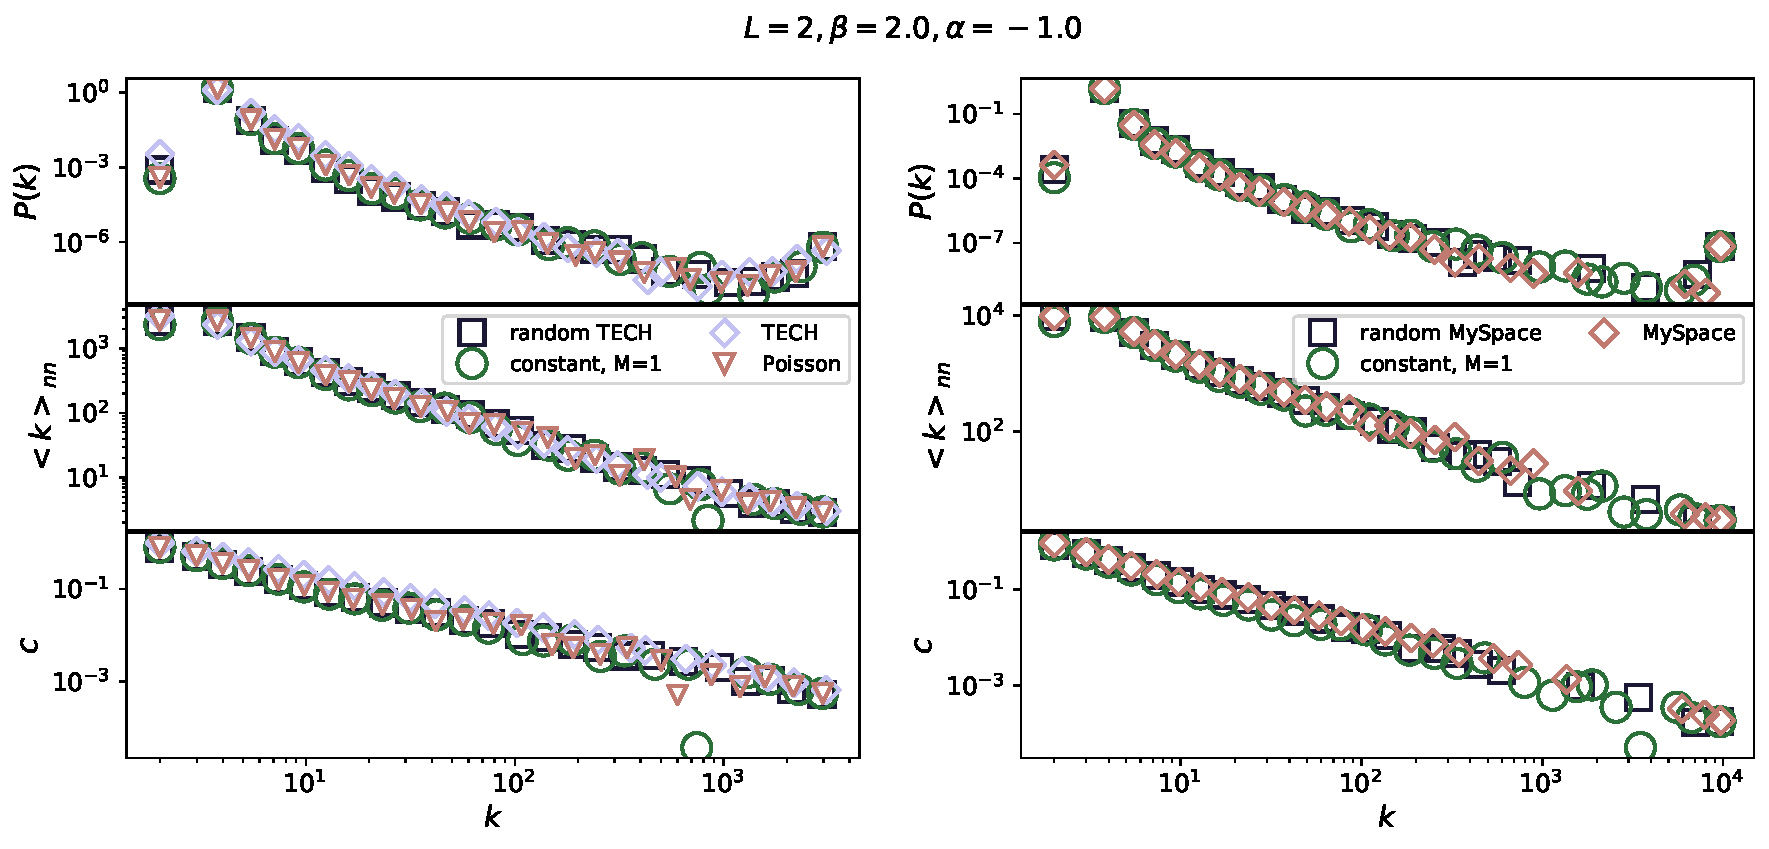
\includegraphics[width=0.9\textwidth]{b2.pdf}
	\caption[Structural properties of networks.]{Degree distribution, the dependence of average first neighbor degree on node degree, dependence of node clustering on node degree for networks grown with different time-varying and constant signals. Model parameters have value $\alpha=-1.0$, $\beta=1.5$  and $L=2$ for all networks. The networks are from scale-free class. Model parameters have value $L=2, \alpha=-1.5$, $\beta=1.5$. The networks have stretched exponential degree distribution. Model parameters have value $ L=2, \alpha=-1.0$, $\beta=2.0$. Generated networks have small-world properties.}
	\label{fig:properties_net}
\end{figure}

\section{Long range correlated signals}

The previous section showed that the growth signal of real systems has complex dynamics. Besides long-range correlations, we also find multifractal properties, and it is hard to isolate individual effects and analyse their influence separately from each other. When this is the case, synthetic signals with specific characteristics can help to verify our findings in real systems. The long-range correlated properties can be included into time series using Fourier filtering transform method \cite{makse1996method}. 

The long range correlated data have power-law correlations $C(s)= <x_i x_{i+s}> = s ^ {-\gamma}$ characterized with coefficient $\gamma$. Hurst exponent depends on $\gamma$ as  $H = 1- \frac{\gamma}{2}$. The Fourier transform, gives us the power spectrum of the time series $S(f)$, that is function of the frequency $f$. For the long-range correlated data it depends on coefficient $\beta = 1-\gamma$ and has form:
\begin{equation}
S(f) \sim f^{-\beta}
\end{equation}
We can generate the data using Fourier filtering with $\beta = 2H - 1$, as following:

\begin{itemize}
	\item first generate one-dimensional sequence of uncorrelated random numbers $u_i$ from Gaussian distribution with $\sigma=1$
	\item calculate the Fourier transform of the generated sequence, $u_q$, the spectrum is flat as data correspond to white-noise
	\item then filter the power spectrum with $f^{-\beta/2}$, so the function will follow power spectrum expected for data with long-range correlations. 	
	\item  calculate the inverse Fourier transform $x_i$. It transforms data to the time domain where signal has desired long range correlations 
	 
\end{itemize}     

The Fourier filtering method generates the Gaussian distributed data, so data are without broad distributions, nonlinear or multifractal properties. Using this method we generated the signals for differet values of the Hurst exponent, see figure \ref{fig:monofractals}. The obtained signals are round to integers and mean values of signals are close to $4$.

\begin{figure}[ht!]
	\centering
	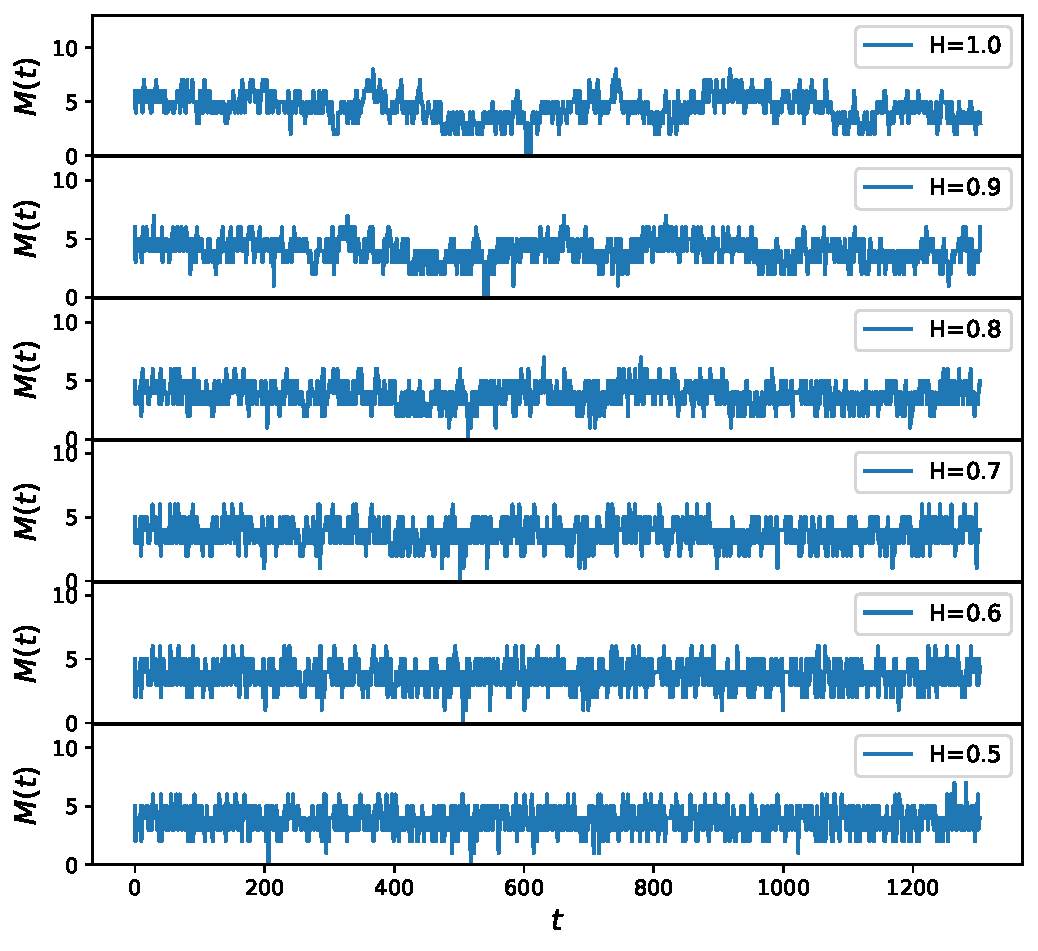
\includegraphics[width=0.6\linewidth]{monofractals.pdf}
	\caption[Long range correlated monofractal signals]{Monofractal signals generated with Fourier filtering method for different Hurst exponents}
	\label{fig:monofractals}
\end{figure}  


As before, we focus on the region of model phase diagram with negative $\alpha$ and positive $\beta$ as there is found the transition line from stretched-exponential across scale-free to the small world- gel networks. We take range of parameters  $-3\leq\alpha\leq-0.5$ and $1\leq\beta\leq3$ with steps $0.5$ and we also vary the the number of links each new node can create $L\in{1, 2, 3}$. For each combination of $(\alpha, \beta, L)$ we generate the sample of $100$ networks, and compare the structure of network grown with fluctuating signals with different Hurst exponent $H \in \{0.5, 0.6, 0.7, 0.8, 0.9, 1.0\}$ and constant signal $M=4$. The results represented by D-measure, shown in the figure \ref{fig:Ddist_m}  are obtained averaging the D-measure between all possible pairs of generated networks.   

The higher values of D-measure are found in the region of critical line $\beta(\alpha^{*})$. The most considerable influence is on networks with scale-free distribution. Comparing D-distance in only one point of  phase diagram, for example $L=1, \alpha = -2.5, \beta = 2.5$, we find that when Hurst exponent is larger, correlations in the signal make bigger impact on the network structure. D-measure between networks grown with signal with Hurst exponent $H=1.0$ and constant signal is $D(H=1.0, M=4) = 0.405$, while between networks grown with signal with $H=0.8$ and constant signal is $D(H=0.8, M=4) = 0.316$. For $\alpha>\alpha^{*}$ networks have similar structural properties and D-measure is close to 0. In the region of networks with stretched exponential degree distribution $\alpha<\alpha^{*}$  differences are small. 

\begin{figure}[H]
	\centering
	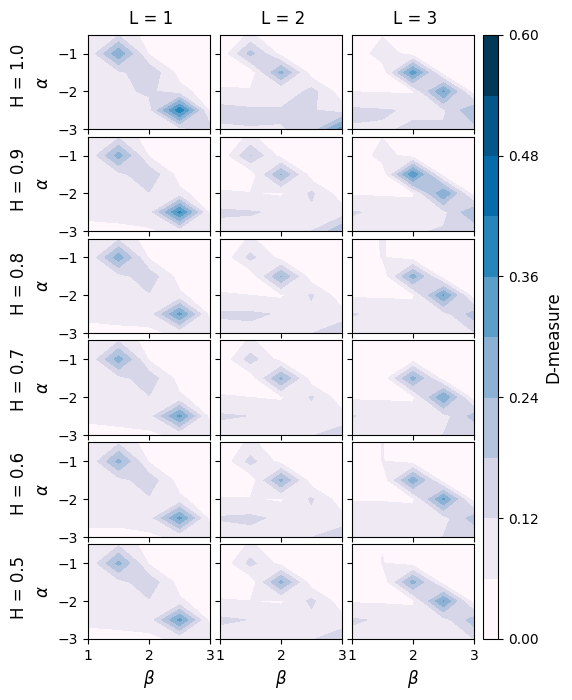
\includegraphics[width=0.6\textwidth]{Ddist_M4_w10.5_w20.5.png}
	\caption[D-distance for networks generated with monofractal signals. ]{D-distance between networks generated with different long-range correlated signals with fixed value of Hurst exponent and networks generated with constant signal M=4.}
	\label{fig:Ddist_m}
\end{figure}


We further explore the assortativity index and clustering coefficient of generated networks. On figure \ref{fig:aindex} are results for several ageing model parameters that show the difference between networks this model can produce. All networks are disassortative, with a negative degree-degree correlation index. For the values of parameters below critical line, $\alpha=-2.5, \beta=1.5$ $r$ does not depend on the Hurst exponent. Above the critical line are small-world networks. They are disassortative. The minimum value of the assortativity index is $r =-1$, for $L=1$, indicating the presence of hubs connecting many nodes. The assortativity index slightly grows with link density. 

In the region of critical parameters, the assortativity index depends on the value of the Hurst exponent. The larger influence on the assortativity index have correlated signals, with Hurst exponent $H>0.8$, so networks become more disassortative, see line for parameters $L=1, \alpha=-2.5, \beta=2.5$ in Figure \ref{fig:aindex}. The long-range correlations have a stronger effect on the evolution of networks with lower density. 

\begin{figure}[h!]
	\centering
	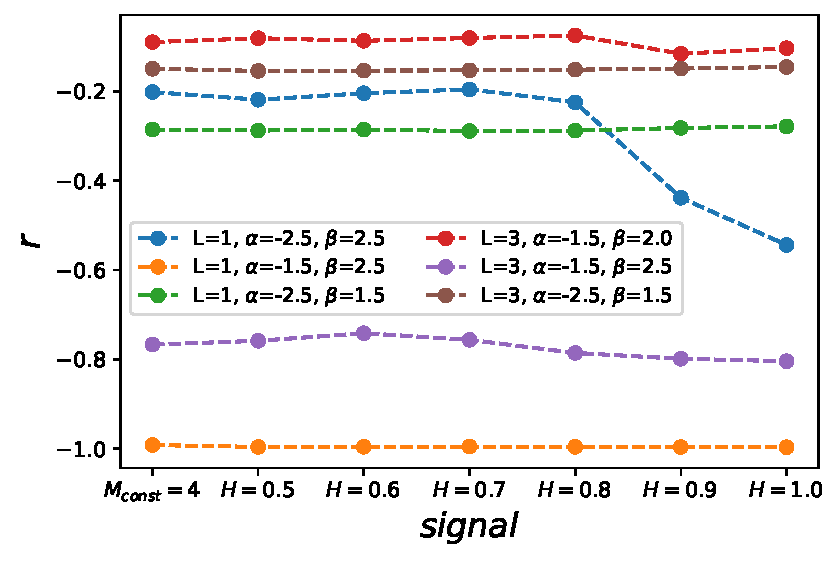
\includegraphics[width=0.45\textwidth]{aindex.pdf}
	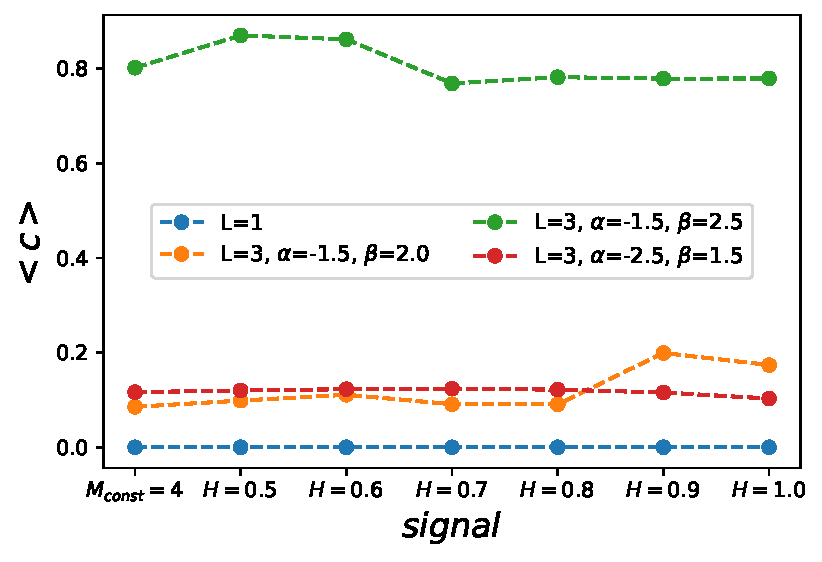
\includegraphics[width=0.45\textwidth]{clustering.pdf}
	\caption[Assortativity index and mean clustering coefficient.]{Mean assortativity index for networks generated with different with different model parameters $\alpha, \beta, L$ and different long-range correlated signals with Hurst exponent $H$.}
	\label{fig:aindex}
\end{figure} 

Figure \ref{fig:aindex} shows the mean clustering coefficient. For $L=1$, networks are uncorrelated trees, with clustering coefficient $0$. For network density $L>1$, nodes are organized into clusters. Under the critical line, for parameter  $L=3, \alpha=-2.5, \beta=1.5 $, clustering coefficient is constant and low. Similar values are obtained for clustering coefficient for critical parameters $L=3, \alpha=-1.5, \beta=2.0$, but for Hurst exponent $H>0.8$ clustering coefficient increase. Small world networks,  $L=3, \alpha=-1.5, \beta=2.5$ are clustered, the value of $<c>$ is high.  The value of clustering for networks created with the constant signal is 0.8. Networks grown with white noise signal and signal with H=0.6 have higher clustering values, while networks grown with signals with a Hurst exponent larger than 0.6 have the same clustering value, below 0.8. 

\section{Conclusions}

In this chapter, we focused on the properties of growth signals and their influence on the system. The network grows at a constant rate in the simplest complex network models. In reality, growth signals are not constant, they are temporally correlated, and the main question is what impact they have on the complex networks. We combined the ageing model with nonlinear growth, while we used real and computer-generated long-range correlated signals for growing signals. The network structure depends on the type of the signals.

The ageing model can generate different complex networks depending on the model parameters. Our results showed that the most significant difference between networks generated with a constant and fluctuating signal is found on the critical line, where networks have broad degree distribution. While temporal correlations do not affect the degree distribution, the networks generated with fluctuating signals are more clustered and have more significant degree-degree correlations. The D-measure indicates that structural differences exist even for networks generated with white noise. For multifractal signals, we find the larger values of the D-measure. Furthermore, if we focus only on monofractal signals, characterized by the fixed value of Hurst exponent, $H$, the difference between networks rises with $H$. 

Away from the critical line in the region of the critical line, the fluctuations do not have a strong influence on the network structure; D-measure is close to zero. In small-world networks, super-hubs emerge, and no matter how strong correlations, trends or cycles exist in the signal, the structure of small-world networks does not change. Similar conclusions are found under the critical line, where networks with stretched exponential degree distribution appear. As $\alpha<<\alpha^{*}$, the new nodes attach to close ancestors, and monofractals do not impact the network structure. Only signals with multifractal properties may contribute to the formation of hubs, which is reflected in larger D-measure between networks. 

Previous research on temporal networks \cite{holme2012} has shown that edge activation properties impact the complex system's dynamics. Also, different studies indicated the importance of fluctuating signals. Our results imply that modelling the social and technological networks should include non-constant growth. In combination with local linking rules, the properties of growth signals can significantly alter the network structure. 

%----------------------------------------------------------------------------------------



\chapter{The growth of social groups}
\label{Ch:Groups}

\section{Social groups}

Two popular online platforms, \textbf{Reddit} and \textbf{Meetup}, are organized into different groups. On Reddit \footnote{https://www.reddit.com/}, users create subreddits, where they share web content and discussion on specific topics, so their interactions are online through posts and comments. The Meetup groups \footnote{www.meetup.com} are also topic-focused, but the primary purpose of these groups is to help users in organizing offline meetings. As meetings happen face-to-face, Meetup groups are geographically localized, so we'll focus on groups created in two towns, London and New York. 

The Meetup data cover groups created from $2003$, when the Meetup site was founded, until $2018$, when we downloaded data using the Meetup API. We extracted the groups from London and New York that were active for at least two months. There were 4673 groups with 831685 members in London and $4752$ groups with 1059632 members in New York. For each group, we got information about organized meetings and users who attended them. From there, for each user, we can find the date when the user participated in a group event for the first time; it is considered the date when the user joined a group. 

The Reddit data were downloaded from the https://pushshift.io/ site. This site collects posts and comments daily; data are publicly available in JSON files for each month. The selected subreddits were created between 2006 and 2011, and we filtered those active in 2017. We removed subreddits active for less than two months. The obtained dataset has 17073 subreddits with $2 195 677$ active members. For each post, we extracted the subreddit-id, user-id and the date when the user created the post. Finally, we selected the date when each user posted on each subreddit for the first time. 

\subsection{The empirical analysis of social groups}

We have information about when the user attended the group event for each Meetup group. In contrast, we have detailed data about user activity for the subreddit, so we can extract the information when a user creates a post for the first time. Those dates are considered as the timestamp when a user joins to group. So both datasets have the same structure: $(g, u, t)$, where $t$ is the timestamp when user $u$ joined group $g$. For each time step, we can calculate the number of new members in each group $N_i(t)$, and the group size $S_{i}(t)$. The group size at time step $t$ is $S_{i}(t)=\sum^{k=t}_{k=t_{0}}N_{i}(t)$, where $t_0$ is month when group is created. The group size is increasing over time, as we do not have information if the user stopped to be active. Also, we calculate the growth rate as the logarithm of successive sizes $R = log(S_{i}(t)/S_{i}(t-1))$.

\begin{figure}[h]
	\centering
	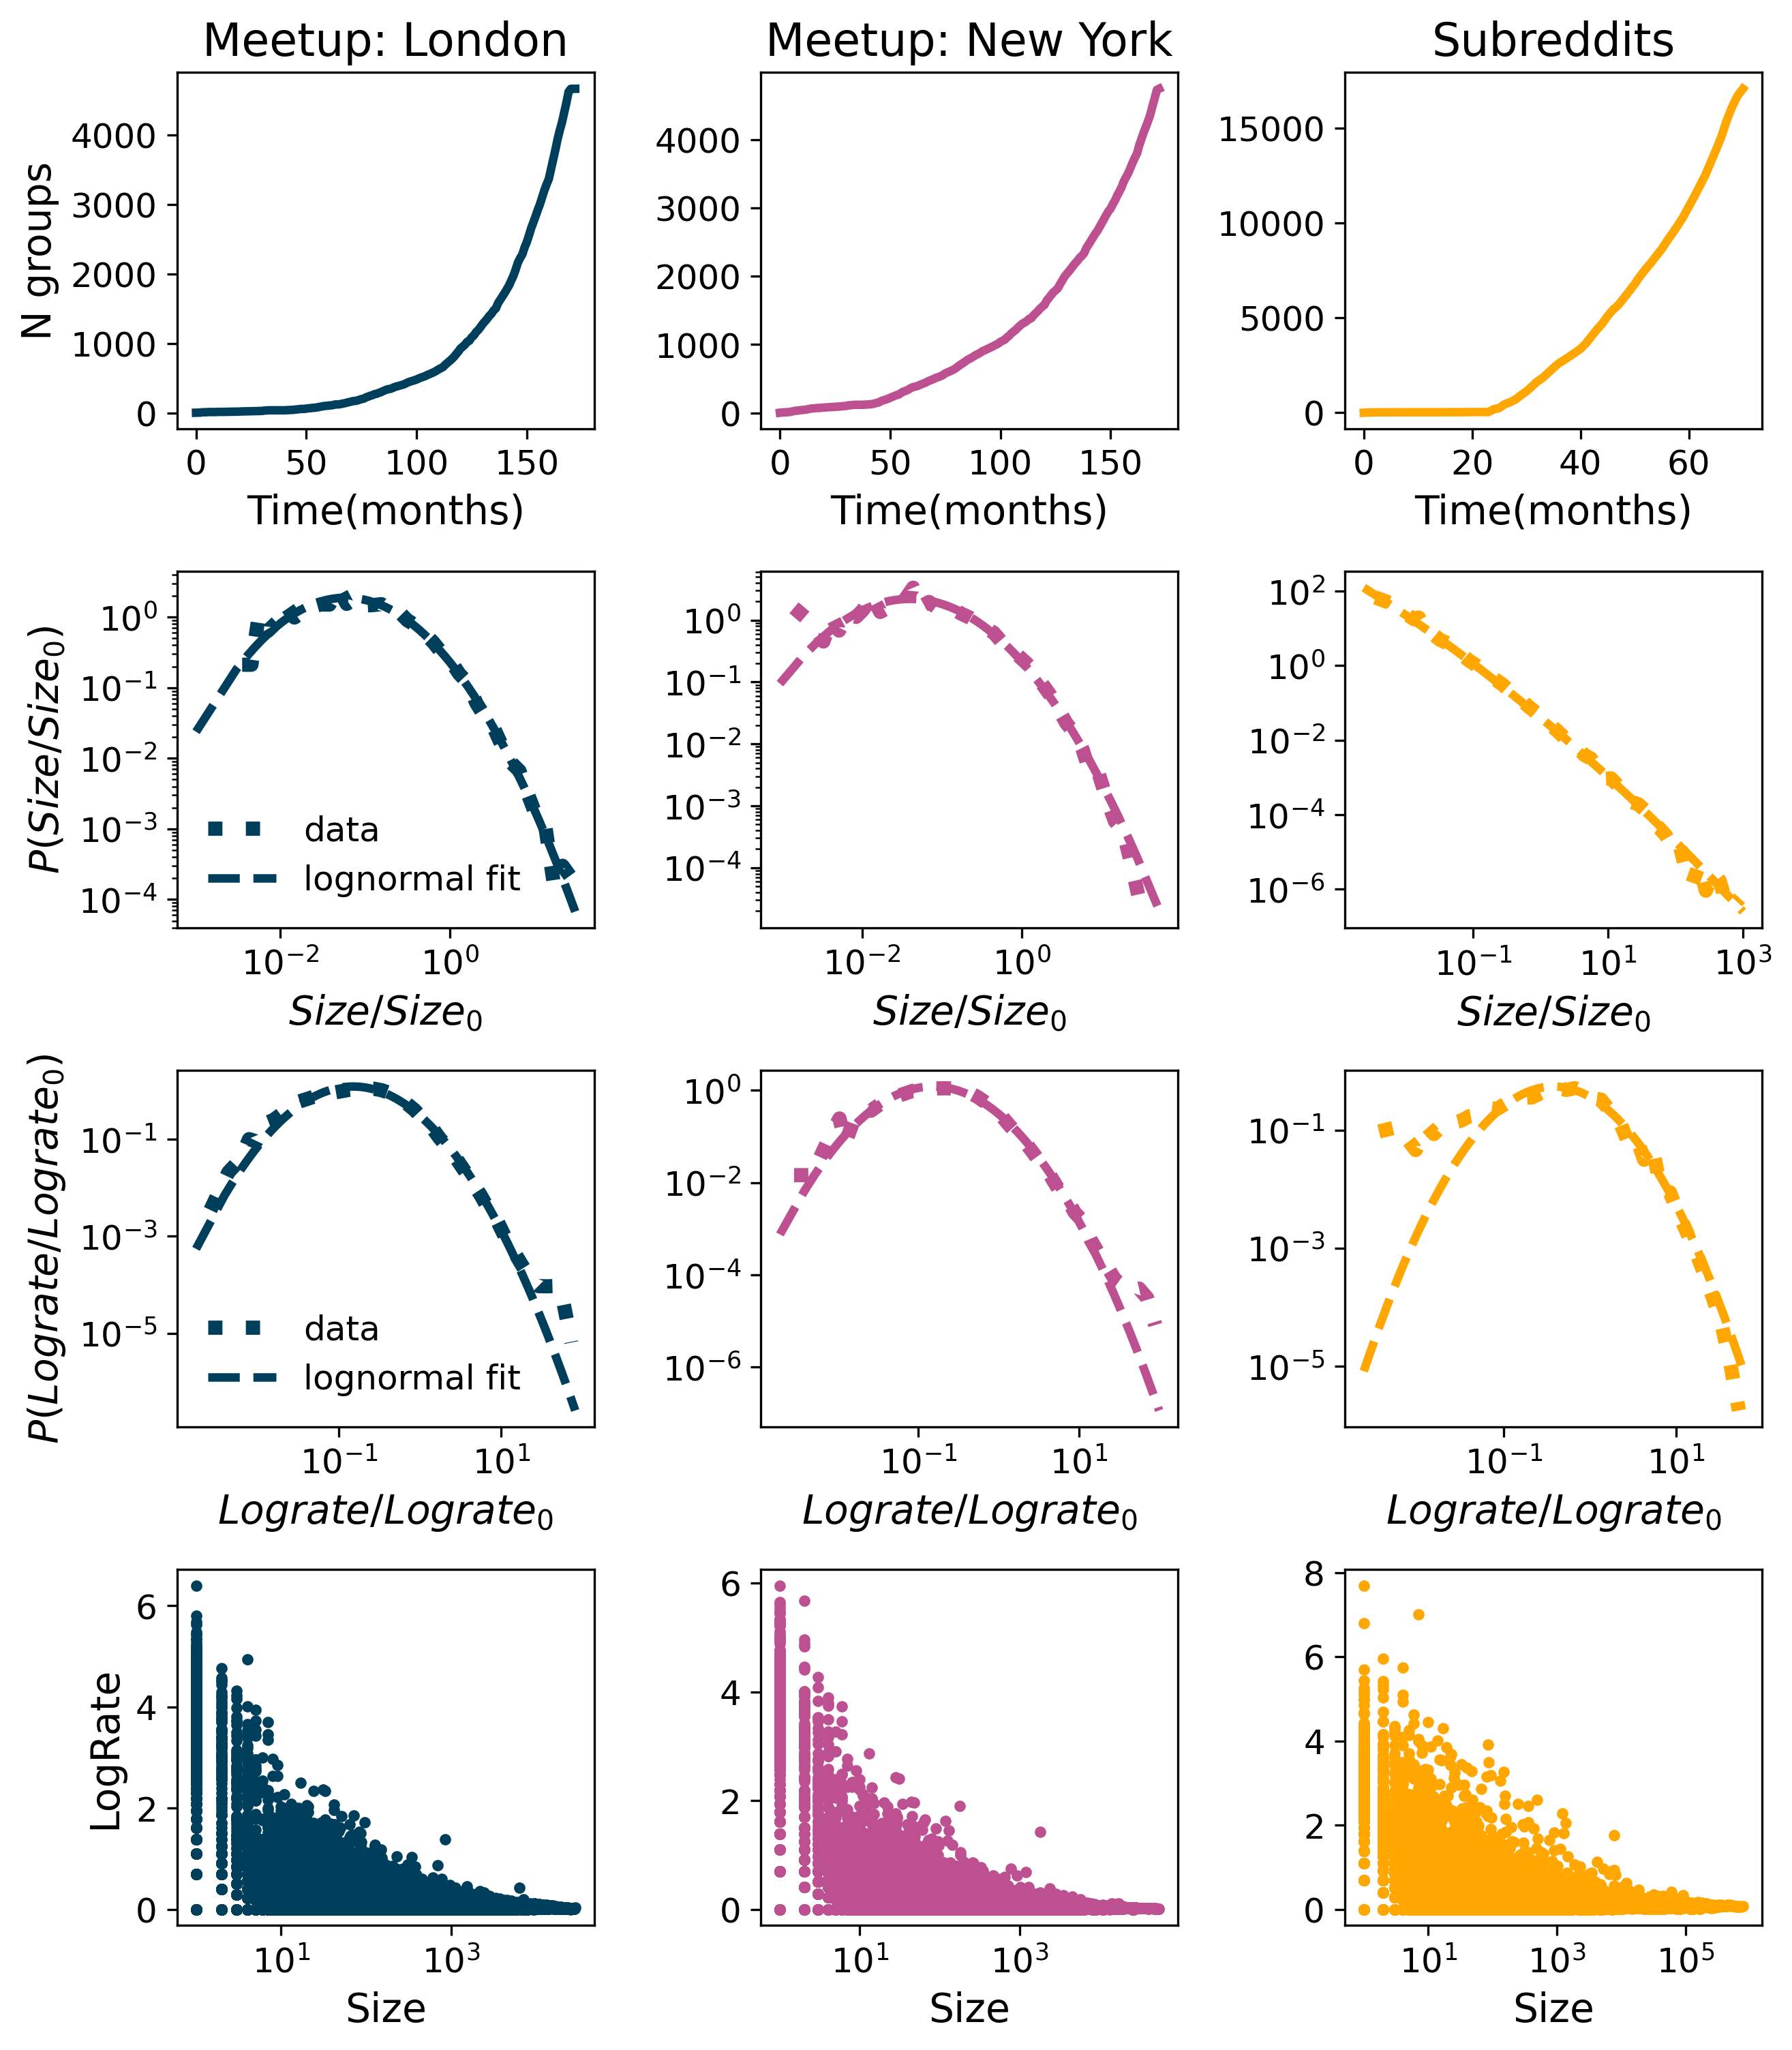
\includegraphics[width=0.8\linewidth]{Figures/figures/Fig2.png}
	\caption[Properties of Meetup and Subreddit groups]{The number of groups over time, normalized sizes distribution, normalized log-rates distribution and dependence of log-rates and group sizes for Meetup groups created in London from 08-2002 until 07-2017 that were active in 2017 and subreddits created in the period from 01-2006 to the  12-2011 that were active in 2017. }
	\label{fig:data1}
\end{figure}   

Even though Meetup and Reddit are different online platforms, we find some common properties of these systems; see figure \ref{fig:data1}. The number of groups and the number of new users grow exponentially. Still, subreddits are larger groups than Meetups. The distribution of groups sizes follows the lognormal distribution:
\begin{equation}
P(S)=\frac{1}{S\sigma\sqrt{2\pi}}exp(-\frac{(\ln(S)-\mu)^{2}}{2\sigma^{2}})
\label{eq:log}
\end{equation}
where $S$ is the group size and $\mu$, and $\sigma$ are parameters of the distribution.

The distributions for Meetup group sizes in London and New York follow a similar lognormal distribution, with parameters $\mu= -0.93$, $\sigma = 1.38$ for London and $\mu=-0.99$ and $\sigma=1.49$ for New York. The group sizes distribution of Subreddits is a broad lognormal distribution that resembles the power law; it has parameters $\mu= -5.41$ and $\sigma = 3.07$.   Still, we used the log-likelihood ratio method and showed that lognormal distribution is a better fit for these data than the power-law. The Result section is given a detailed analysis that supports these findings.   

The simplest model that generates the lognormal distribution is the multiplicative process \cite{mitzenmacher2004brief}. Gibrat used this model to explain the growth of firms. The main assumption of this model is that growth rates  $R = log\frac{S_t}{S_{t-\Delta t}}$ do not depend on the size $S$ and that they are uncorrelated. Further, this implies the lognormal distribution of the sizes, while the distribution of growth rates appears to be a normal distribution,  \cite{mondani2014fat}, \cite{fu2005growth}. Figure \ref{fig:scale} shows the distribution of the logrates that follow a lognormal distribution, contrary to the Gibrat law. Furthermore, logrates depend on the group size \ref{fig:scale}. For these reasons, the Gibrat law can not explain the growth of online social groups. Similar conclusions are shown in recent studies about cities or the growth of the internet \cite{frasco2014spatially, qian2014origin}.   

The growth of online social groups has universal behavior independent of the group's size. If we aggregate the groups created in the same year $y$, and each group size normalizes with average size $<S^y>$, $s^{y}_{i}=S^{y}_{i}/<S^{y}>$ we will find that group sizes distributions for the same dataset and different years fall on the same line, figure \ref{fig:scale}. The same characteristics are observed for the distribution of the normalized logrates \ref{fig:scale}. The growth is universal over time, and the group sizes distribution does not change from year to year.

\begin{figure}[h]
	\centering
	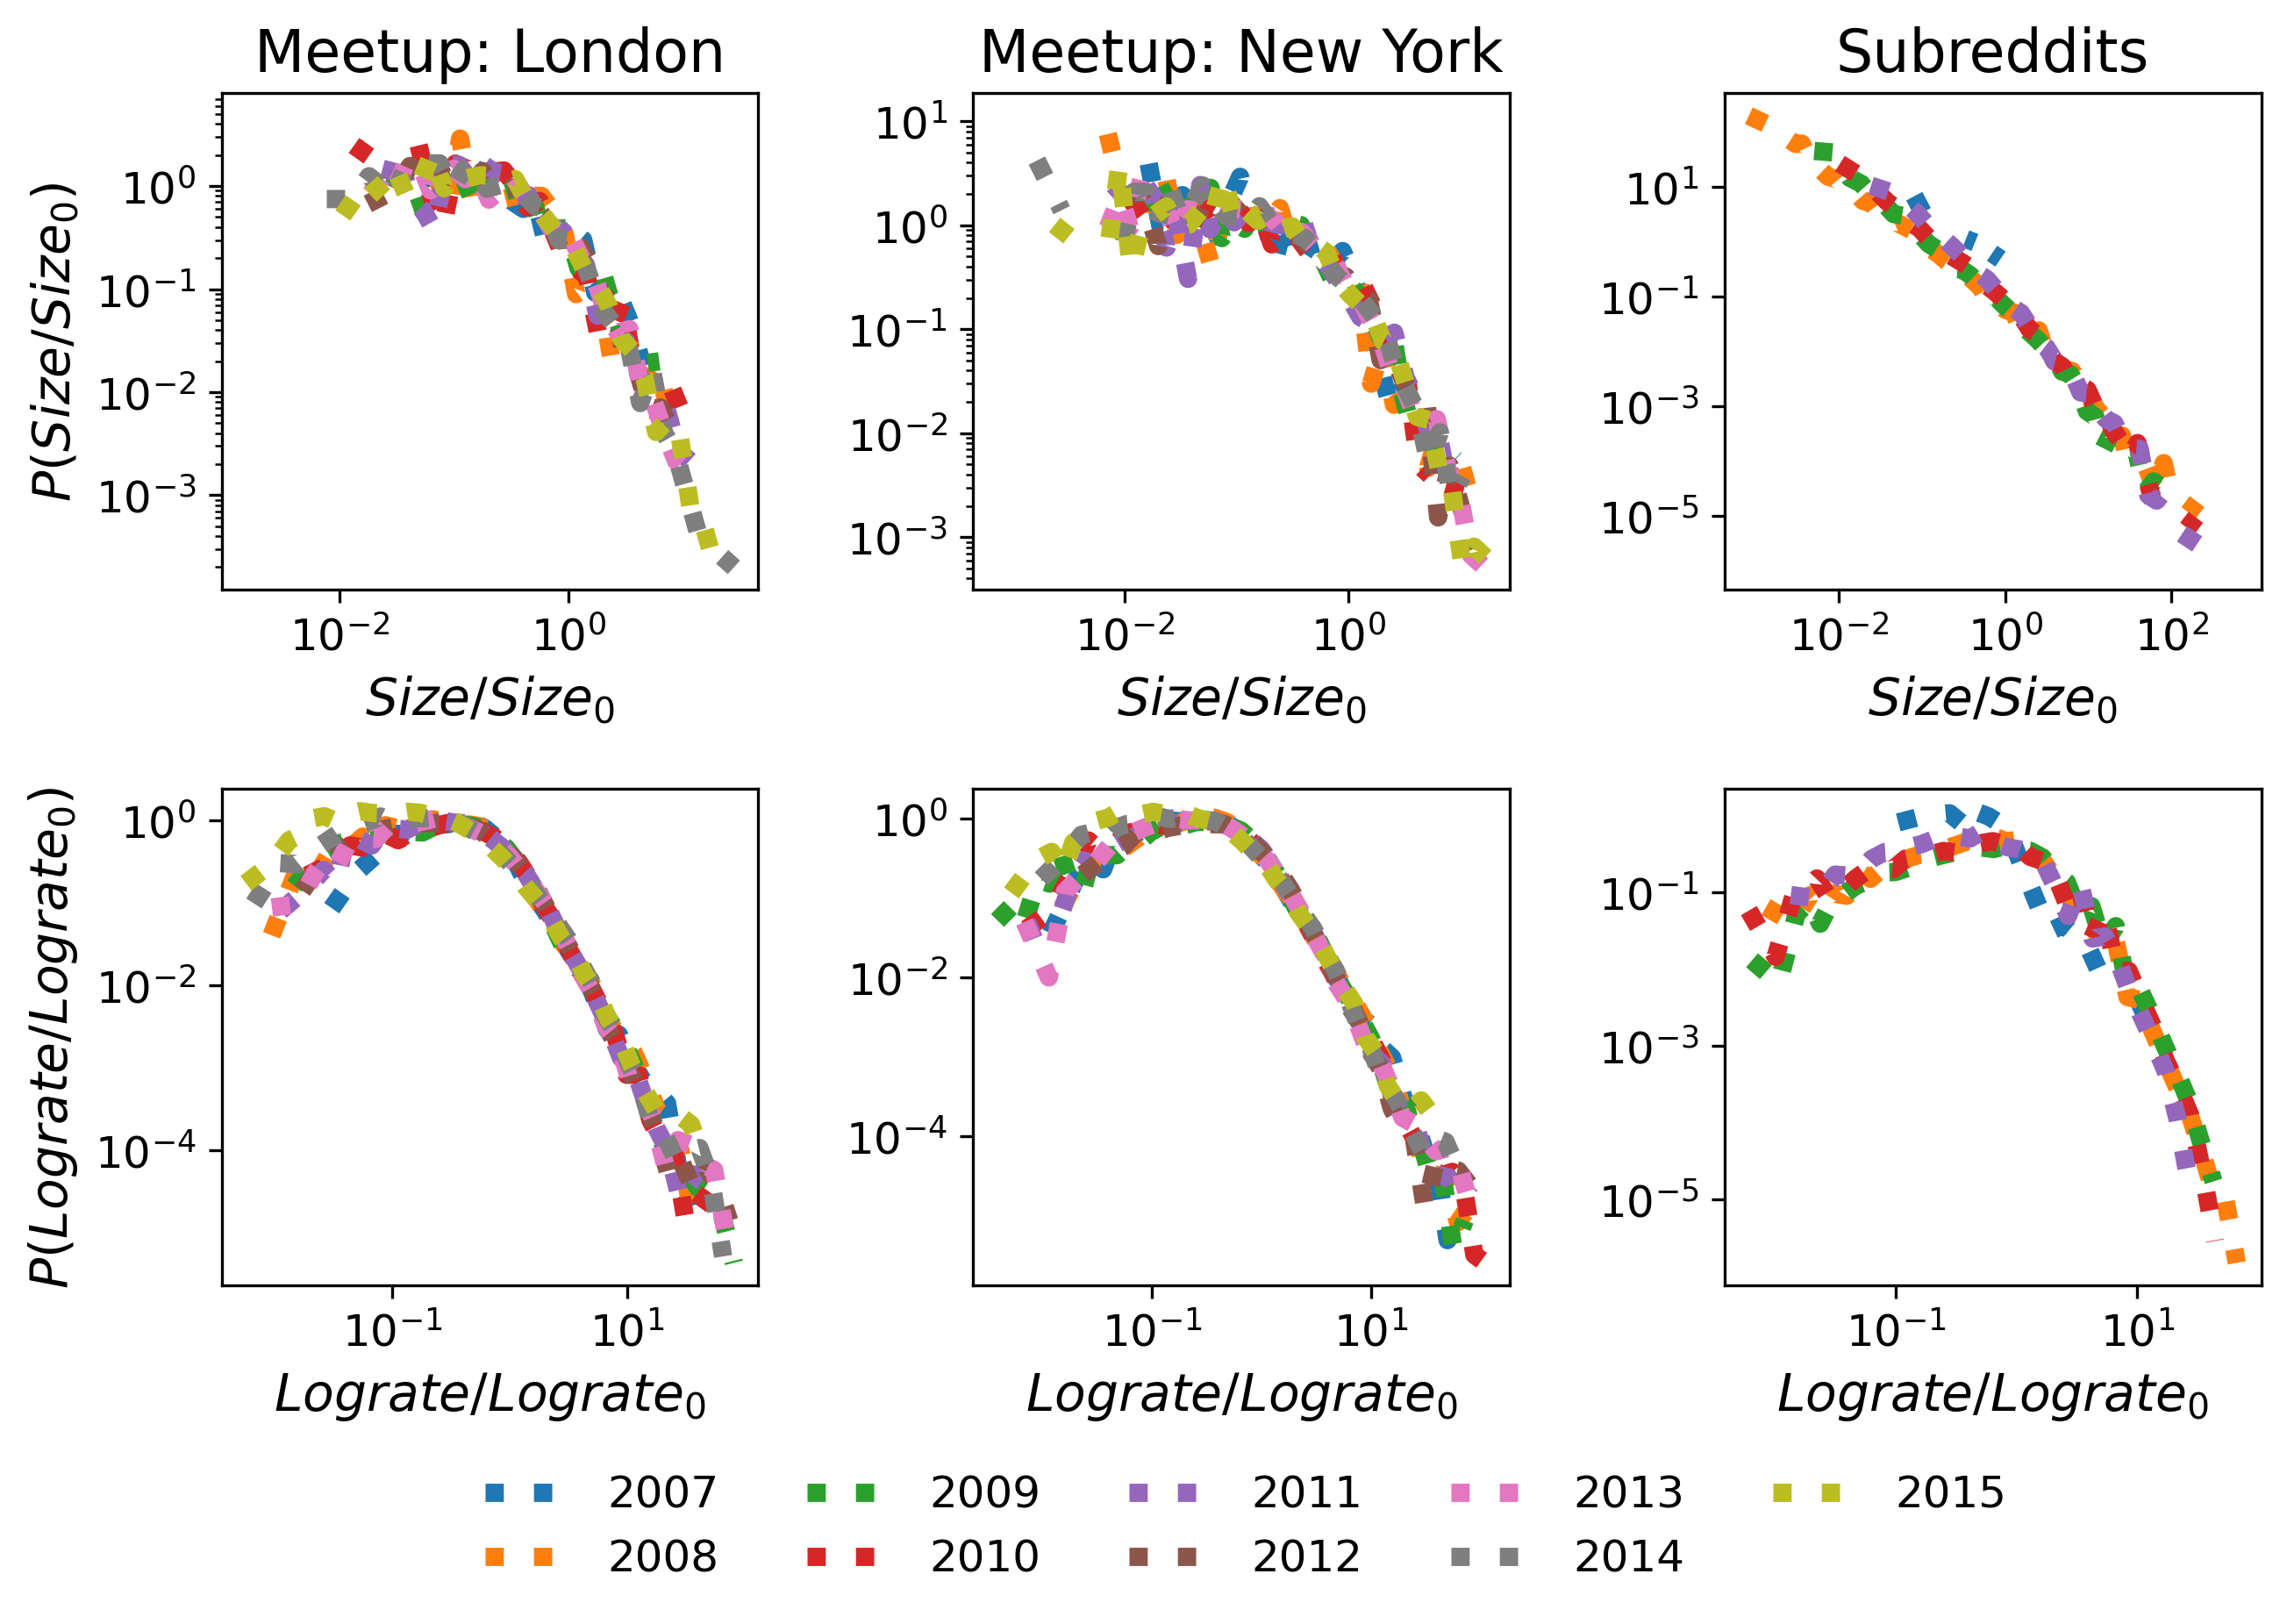
\includegraphics[width=0.8\linewidth]{Figures/figures/Fig1.png}
	\caption[Universality in the Meetup and Reddit groups]{The figure shows the groups' sizes distributions and log-rates distributions. Each distribution collects groups founded in the same year and is normalized with its mean value. The group sizes are at the end of 2017 for meetups and 2011 for subreddits.}
	\label{fig:scale}
\end{figure}
\newpage
\section{The model}

Meetup and Reddit engage members in different activities. Still, there are some underlying processes same in both systems. Each member can create new groups and join existing ones. Both systems grow in the number of groups and users, and each user can belong to an arbitrary number of groups. In the previous section, we identified the universal patterns in the growth of social groups, but the growth can not be modelled with the Gibrat law. 

The complex network models allow us to simulate the growth of these systems considering all types of members' activities. We can identify how model parameters shape growth by varying linking rules.
Regarding the user's group choice, it was shown that social connections play an important role \cite{kairam2012life, zheleva2009co}. On the other hand, users can be driven by personal interests. Diffusion between groups could also be enhanced with rich-get-richer phenomena, where users join larger groups. With a complex network model, we can easily incorporate the nonlinear growth in the number of users and groups, as it is an important parameter that shapes the structure and dynamics of the complex network \cite{mitrovic2011quantitative, dankulov2015dynamics, vranic2021growth}.

The evolution of the social groups has been studied using the co-evolution model in the reference  \cite{zheleva2009co}. This model consists of two evolving networks: the bipartite network, which stores connections between users and groups and the affiliation network of social connections. At each time step, active users create new connections in the affiliation network; i.e. they make new friends. They also join existing groups or create new ones, which updates the bipartite network. The group selection can be random with probability proportional to the group size; otherwise, the group is selected through social contacts. Using this model, authors have reproduced the power-law group size distribution found in several communities, such as Flickr or LiveJournal. The empirical analysis of Meetup and Reddit groups showed that group size distribution could be lognormal, meaning that some different mechanisms control the growth of the groups.

We propose a model that is based on the co-evolution model. The main difference between those two models is how model parameters are defined. First of all, in the co-evolution model user becomes inactive after period $t_a$, which is drawn from an exponential distribution with the rate $\lambda$, while in our model probability that the user is active is constant, and the same for each user. The second difference is how groups are chosen. While in the co-evolution model probability that the user selects a group through social linking depends on the friend's degree, we give preference to groups where a user has a larger number of social contacts. We also modified the rules for random linking so users choose a group with uniform probability.

\subsection{Groups growth model}

The representation of the model is given in figure \ref{fig:schema}. The model consists of two networks:
\begin{itemize}
	\item bipartite network $\mathcal{B}(V_{U}, V_{G}, E_{UG})$, where $V_U$ is set of users, $V_G$ set of groups and $E_{UG}$ set of links between users and groups, where link $e(u,g)$ indicates that user $u$ is member of group $g$.
	\item social network $\mathcal{G}(V_{U},E_{UU})$ describes the social connections $e(u, v)$ between users $u$ and $v$, and  $V(U)$ is set of users same as in bipartite network. 
\end{itemize}

The bipartite and social networks evolve. New users $N_U(t)$ are added to the network at each step. It is how the set of users $V_U$ in the bipartite and social network can grow. At arrival, each new member connects to a randomly selected user in the social network $G$. This allows new members to choose a group based on social contacts \cite{kairam2012life}. The activity of old members is a stochastic process; old members are activated with probability $p_a$. The set of active users $\mathcal{A}_{U}$ has new members $N_U(t)$ and old members who decided to be active in that time step.

The active users can create a new group with probability $p_g$. By this, group node $g$ is added to the set of group nodes $V_G$ in bipartite network $B$. If an active user does not create a new group, it will join the existing one with probability $1-p_g$, see lower panel on figure \ref{fig:schema}. When the user creates a new group or joins an existing one, the link $e(u,g)$ is made in the bipartite network $B$.

\begin{figure}[h]
	\centering
	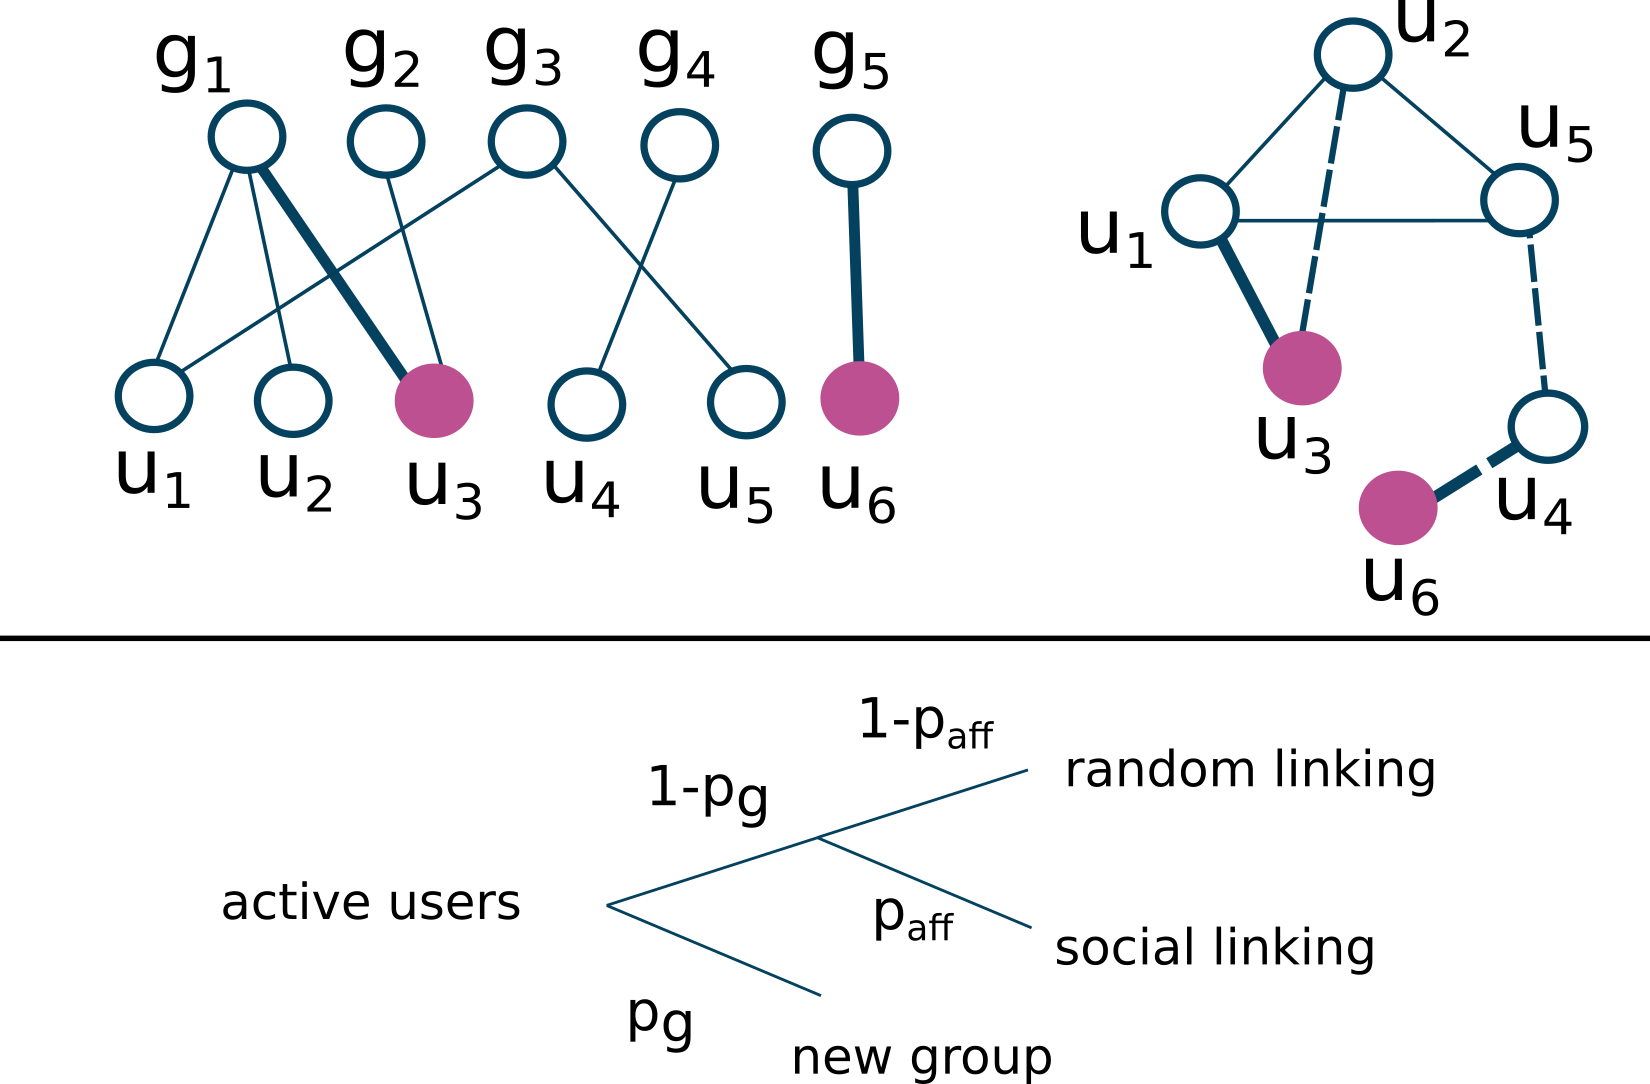
\includegraphics[scale=0.45]{Figures/figures/test.png}
	\caption[Bipartite groups growth model]{The top panel shows bipartite (member-group) and social (member-member) networks. Filled nodes are active members, while thick lines are new links in this time step. In the social network, dashed lines show that members are friends but do not share the same groups. The lower panel shows the model schema, where $p_g$ is the probability that the user creates a new group, while $p_{aff}$ is the probability that group choice depends on social connections. \textbf{Example:} member $u_6$ is a new member. First, it will make a random link with node $u_4$, with probability, $p_g$ makes a new group $g_5$. With probability, $p_a$ member $u_3$ is active, while others stay inactive for this time. Member $u_3$ will, with probability $1-p_g$ choose to join one of the old groups, and with probability $p_{aff}$ linking is chosen to be social. As its friend $u_2$ is a member of group $g_1$, member $u_3$ will also join group $g_1$. When member $u_3$ joins to group $g_1$, it will make more social connections; in this case, it is member $u_1$.}
	\label{fig:schema}
\end{figure}

When joining existing groups, users may be influenced by social connections. This linking happens with probability $p_{aff}$. The second case is that the user chooses a random group with probability $1-p_{aff}$. 

Social linking depends on the properties of a bipartite and social network. The networks can be represented with matrices $B$ and $A$, so if a link between two nodes exists, they have element $1$. The neighbourhood of user $u$, $\mathcal{N}_{u}$ in a bipartite network is a set of groups in which the user is a member. Similarly, we define the neighbourhood of group $g$ as $N_g$, as a set of users who belong to the group. From there, we can define the probability $ P_{ug}$ that the user $u$ will choose group $g$. This probability is proportional to the number of social contacts that the user has in the group. 

\begin{equation}
P_{ug}=\sum_{u_{1}\in \mathcal{N}_{g}} A_{uu_{1}} 
\label{eq1}
\end{equation}

After selecting group $g$, user $u$ is introduced to new members in the group and can make new social contacts. In the simplest case, we could assume that all members belonging to a group are connected. However, previous research on this subject \cite{ smiljanic2017associative, backstrom2006group, zheleva2009co} has shown that the existing social connections of members in a social group are only a subset of all possible connections. We select $X$ random members $u_i$ from a group $g$ and make new connections in the social network $e(u, u_i)$. 

The model parameters $p_a$ and $p_g$ are important for controlling the number of users and groups. With larger parameter values $p_a$, more users become active, and the number of links in bipartite and social networks grows faster. Parameter $p_g$ controls the rate at which new groups are created. For example, if $p_g=0$, users will not create new groups. Also, if $p_g=1$, users will only create new groups, and the resulting network will consist of star-like subgraphs. In real systems, we do not expect extreme values for probabilities $p_a$ and $p_g$. First, not all members are constantly active, and we do not find a burst in the creation of the groups. From real data, we notice that there is always a higher number of users than groups in social systems. The parameter $p_{aff}$ how users choose groups, and with higher $p_{aff}$ social connections become more important. 

\subsection{Dependence of the group size distribution on model parameters}

Before applying the group growth model on Meetup and Reddit, we consider the system where at each time step, a constant number of users is added $N(t)=30$. We also fix the probability that the user is active to $p_a=0.1$, so we can, in more detail, explore the influence of parameters $p_g$ and $p_{aff}$. We plot the group size distribution after the $60$ steps of simulation. The values of $p_g$ and the $p_a$ influence the number of groups, their maximum size, and the shape of group size distribution. With probability $p_g=0.1$, users create a large number of groups, over $10^4$, while with $p_g=0.5$, they are on the order of magnitude $10^5$. 

Figure \ref{fig:n30} show the obtained group size distributions with power-law and lognormal fits. Users join randomly chosen groups for a lower value of parameter $p_g=0.1$ and $p_{aff}=0$. Group size distributions are approximated with lognormal. When the affiliation parameter is larger, $p_{aff}=0.5$, the lognormal distribution becomes broader, and so on, we find the larger maximum group size. If we increase the parameter $p_g=0.5$, every second active user will create a group. At this group creation rate, the group size distribution deviates from lognormal, but it is not explained with power-law either, right column on figure \ref{fig:n30}.

\begin{figure}[H]
	\centering
	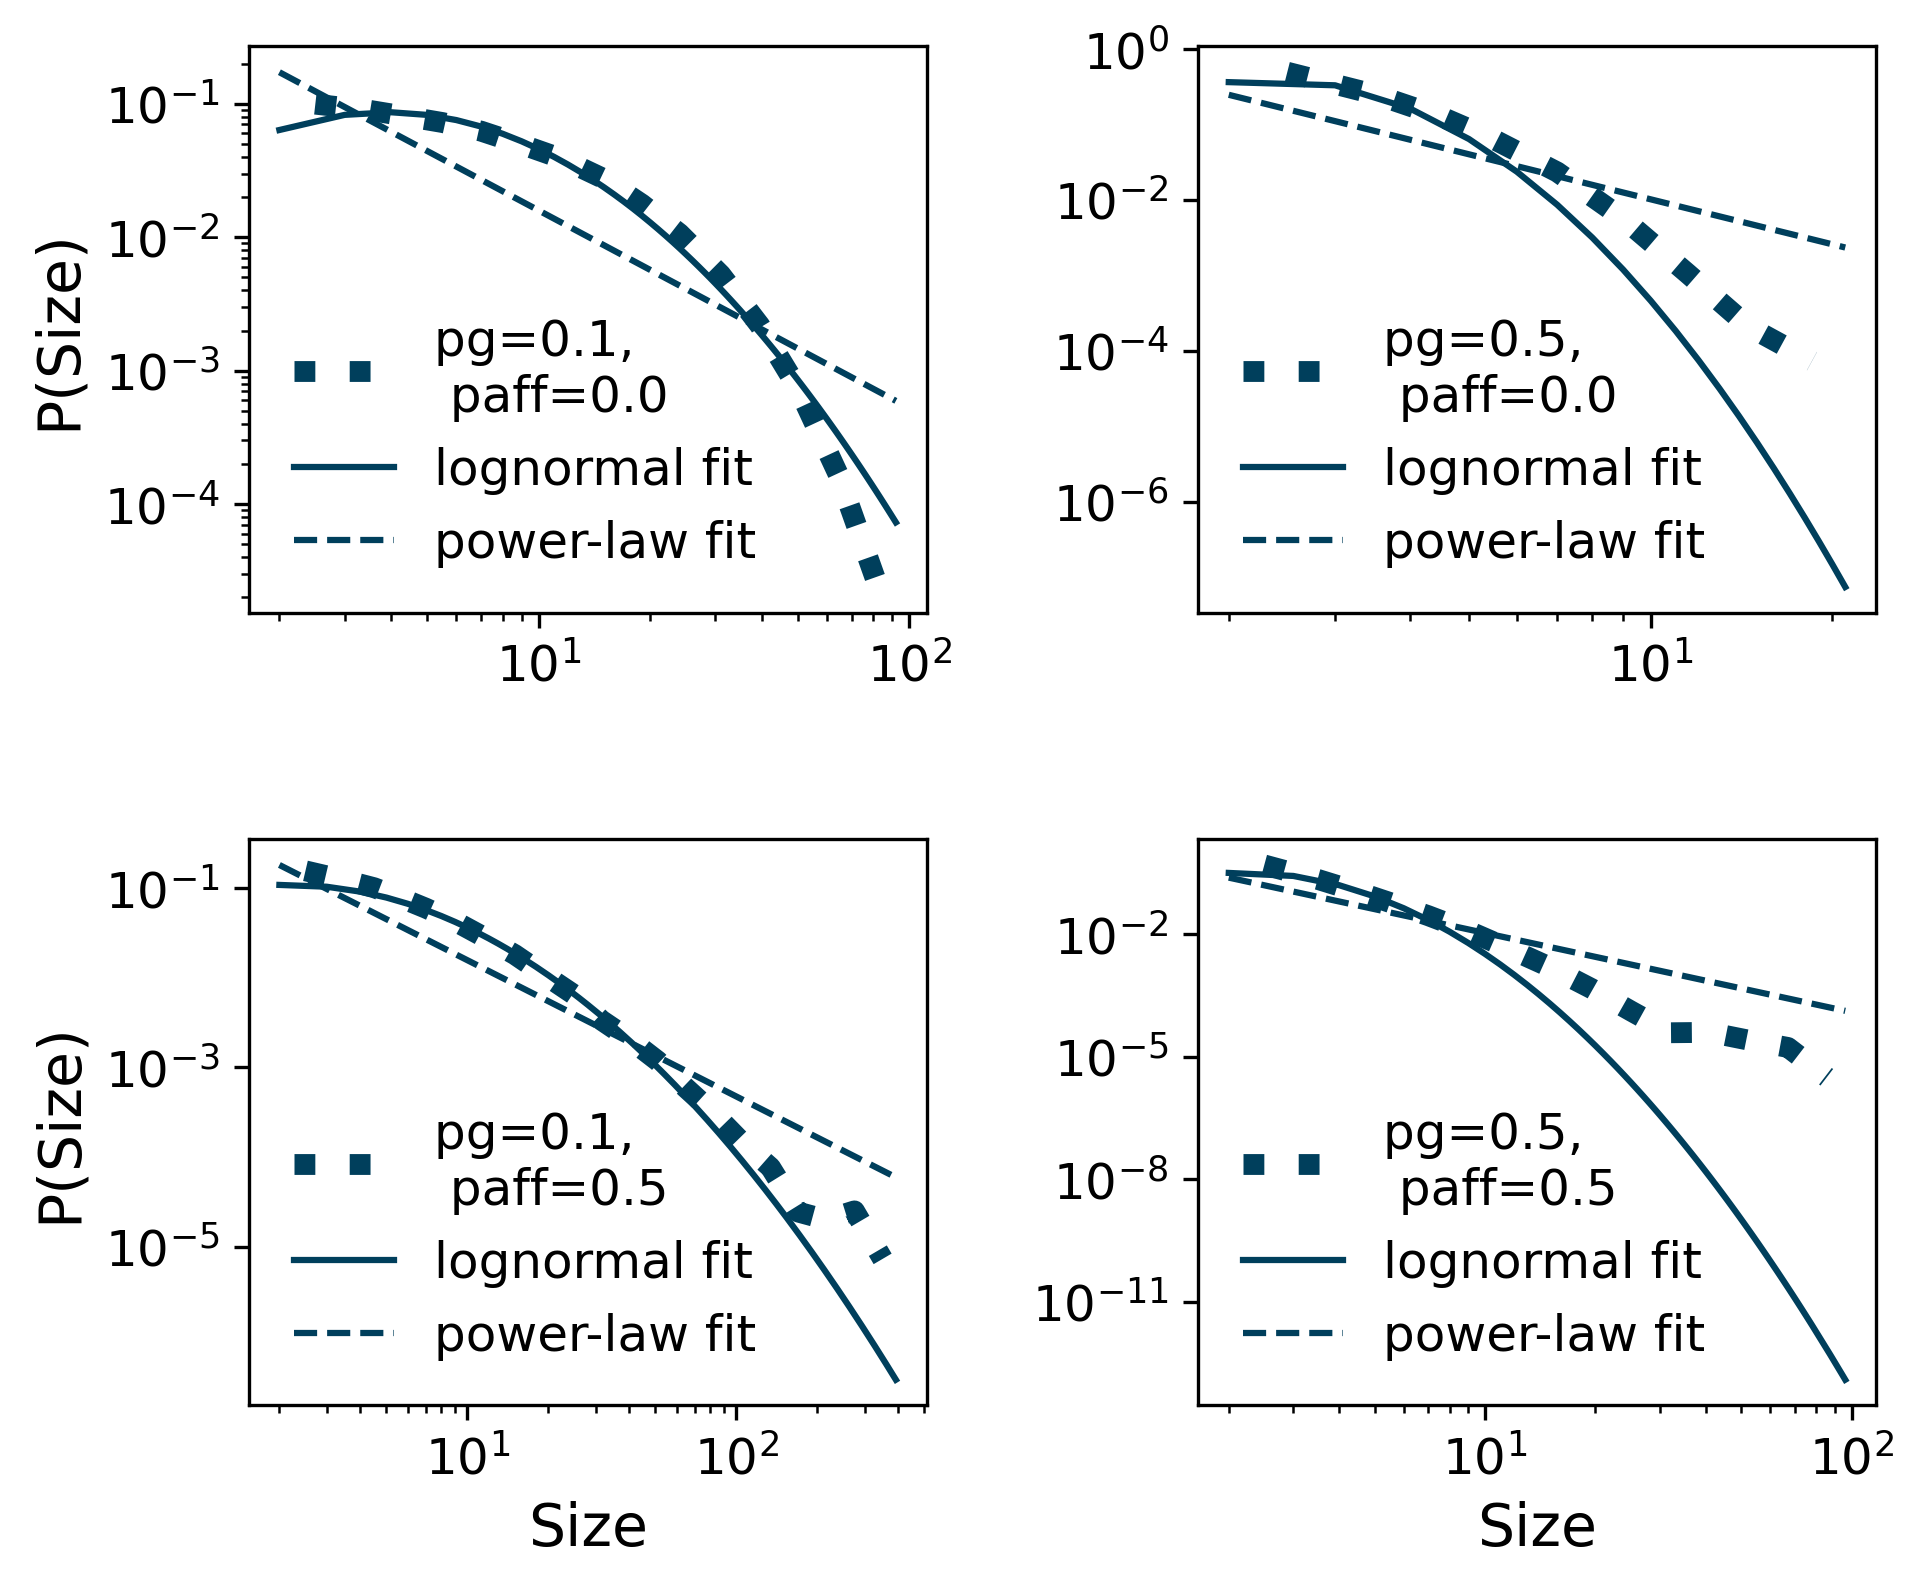
\includegraphics[width=0.6\linewidth]{Figures/figures/Fig5_a.png}
	%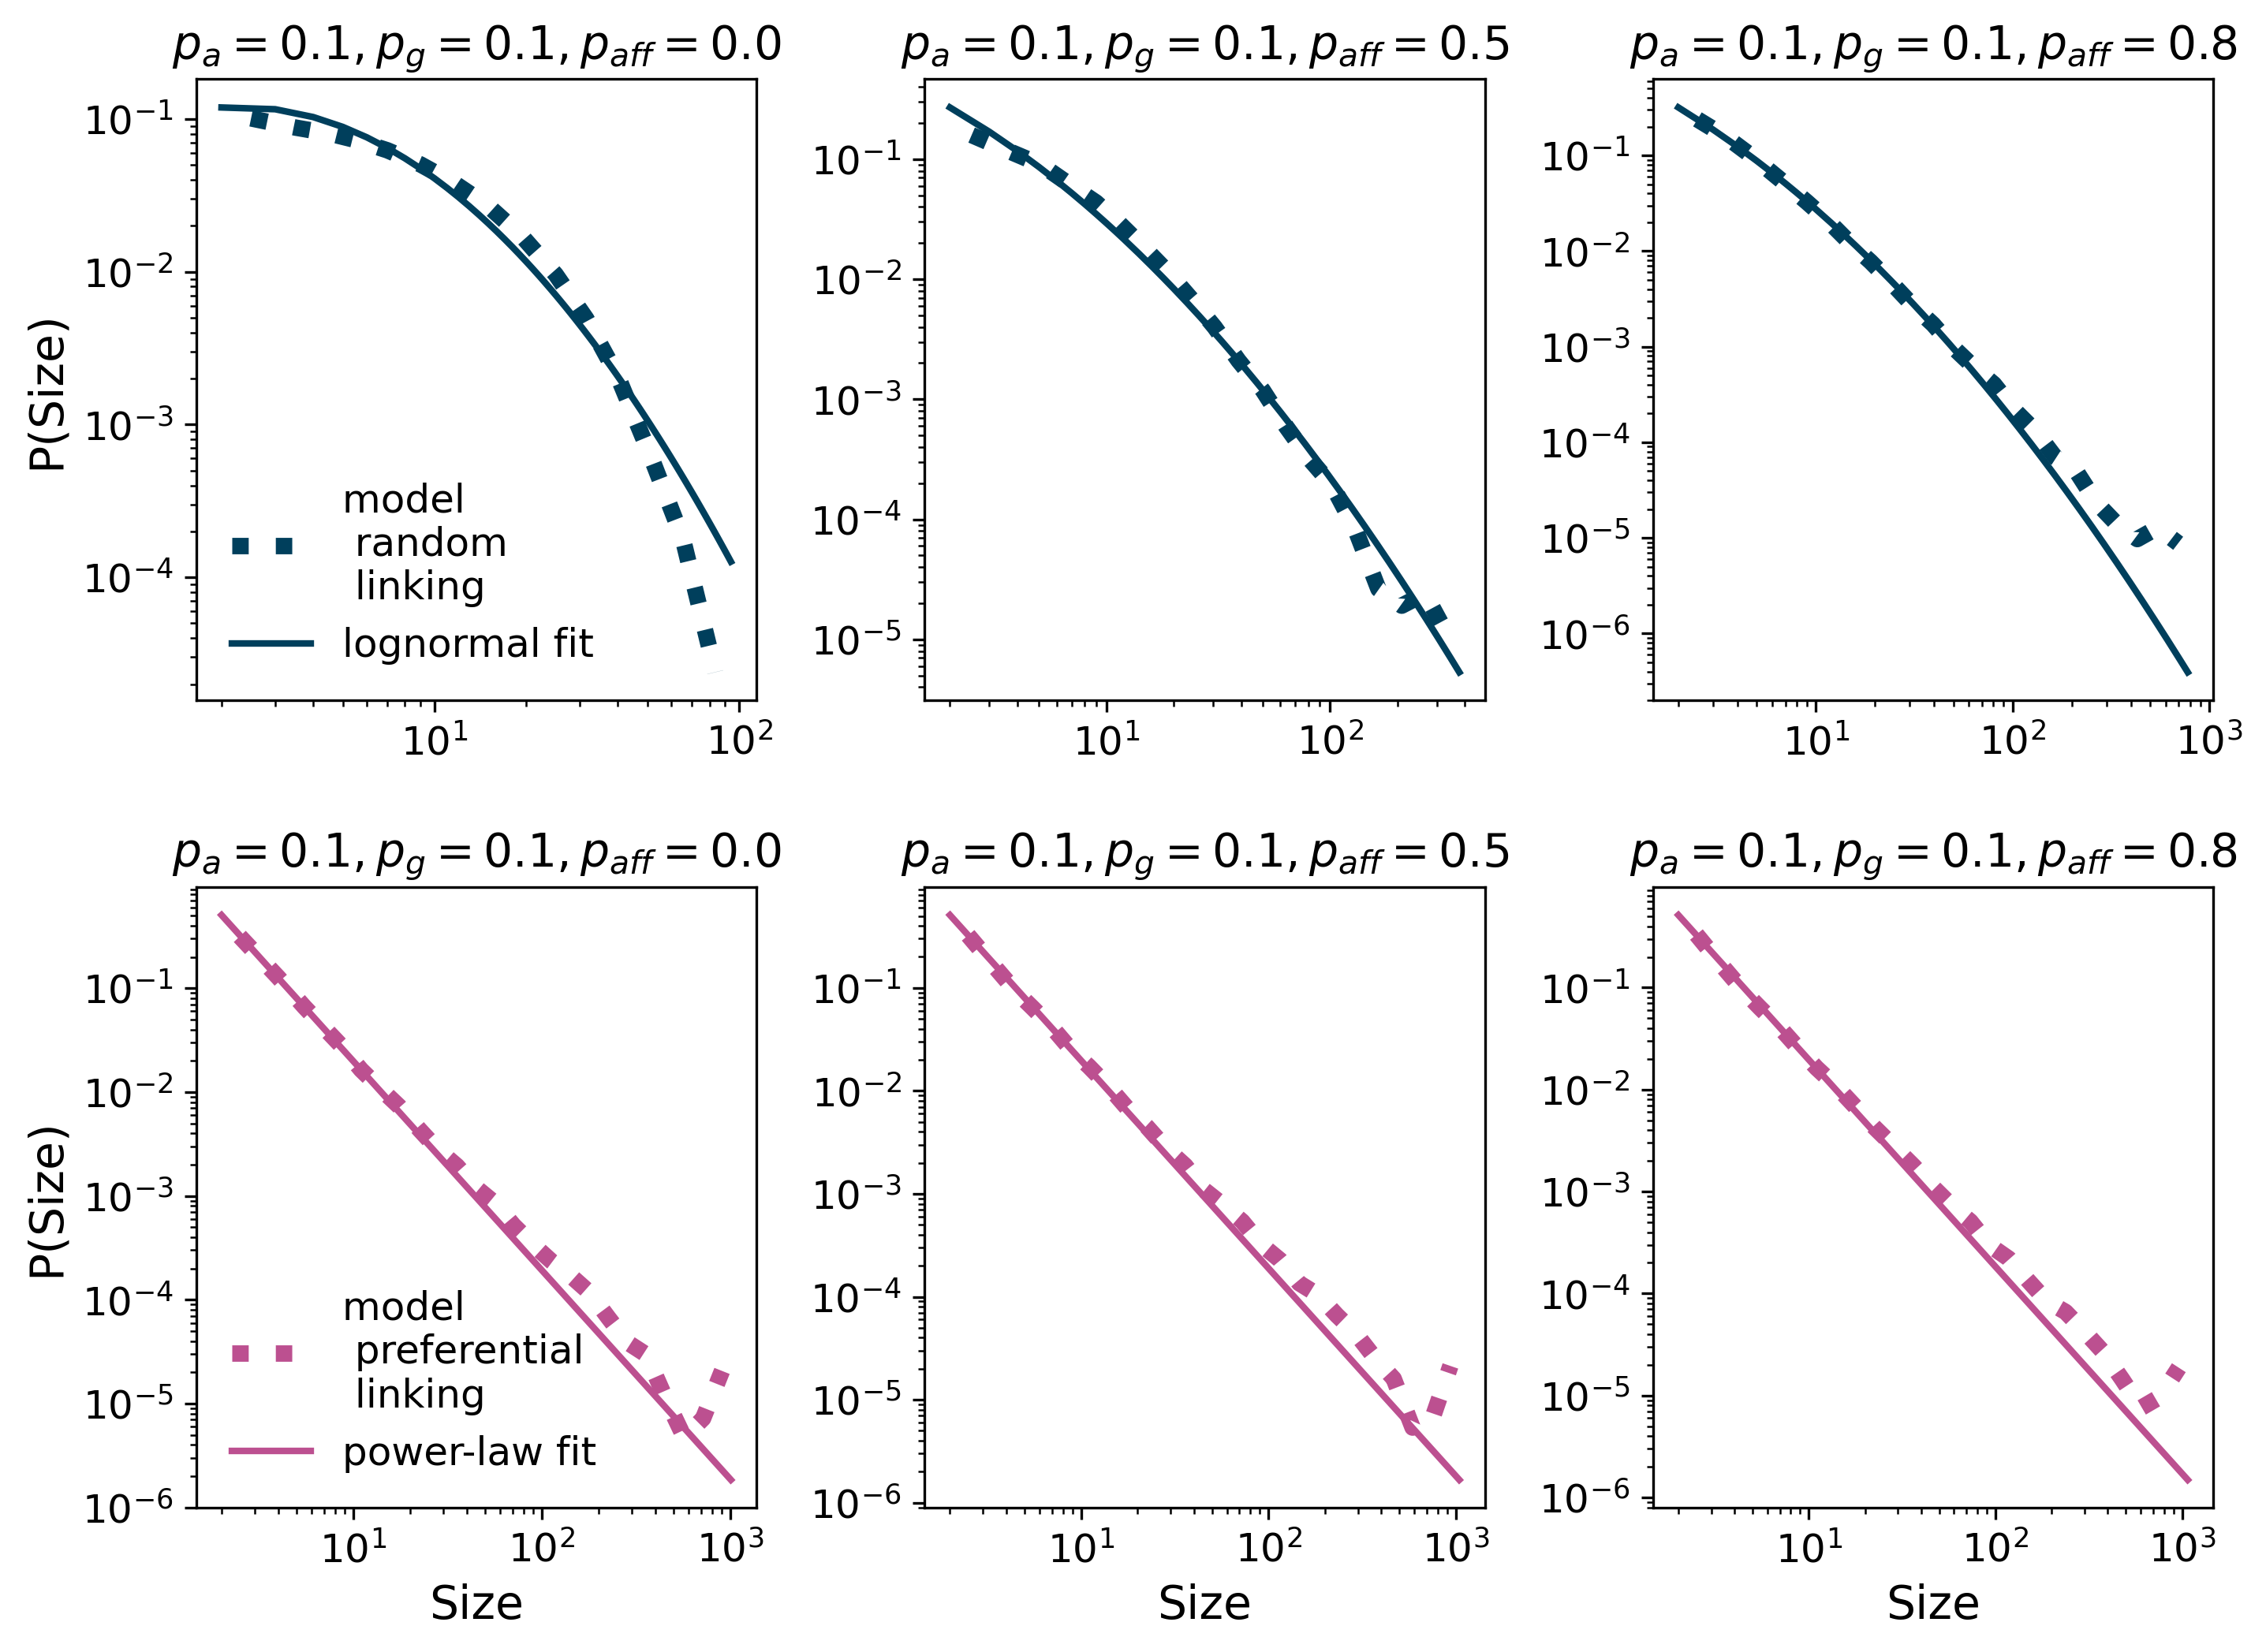
\includegraphics[width=0.8\linewidth]{figures/model_N30.png}
	\caption[Group size distribution for different model parameters]{The distribution of sizes for different values of $p_{g}$ and $p_{aff}$ and constant $p_{a}$ and growth of the system. The combination of the values of parameters of $p_{g}$ and $p_{aff}$ determine the shape and the width of the distribution of group sizes. }
	\label{fig:n30}
\end{figure}

Finally, we compare how group size distribution depends on different rules in random linking. In our model, the probability that the user chooses a random group is uniform. In contrast, in the co-evolution model \cite{zheleva2009co}, probability depends on the group size, as in the preferential attachment model. Instead of random linking, if we incorporate preferential linking, users with probability $1-p_{aff}$ tend to choose larger groups, and group size distribution changes significantly. Similar to the co-evolution model, we find the power-law distribution. Figure \ref{fig:model_comp} shows the results from a model where we add a constant number of new users at each time step. The probabilities $p_a$ and $p_g$ are fixed, and the affiliation parameter takes values $0$, $0.5$ and $0.8$. If we consider random linking, a top panel on figure \ref{fig:model_comp}, the distribution becomes broader with larger $p_{aff}$. On the other hand, with preferential linking, group size distribution is a power law, and the $p_{aff}$ parameter does not have a large impact on the distribution shape.    

\begin{figure}[h]
	\centering
	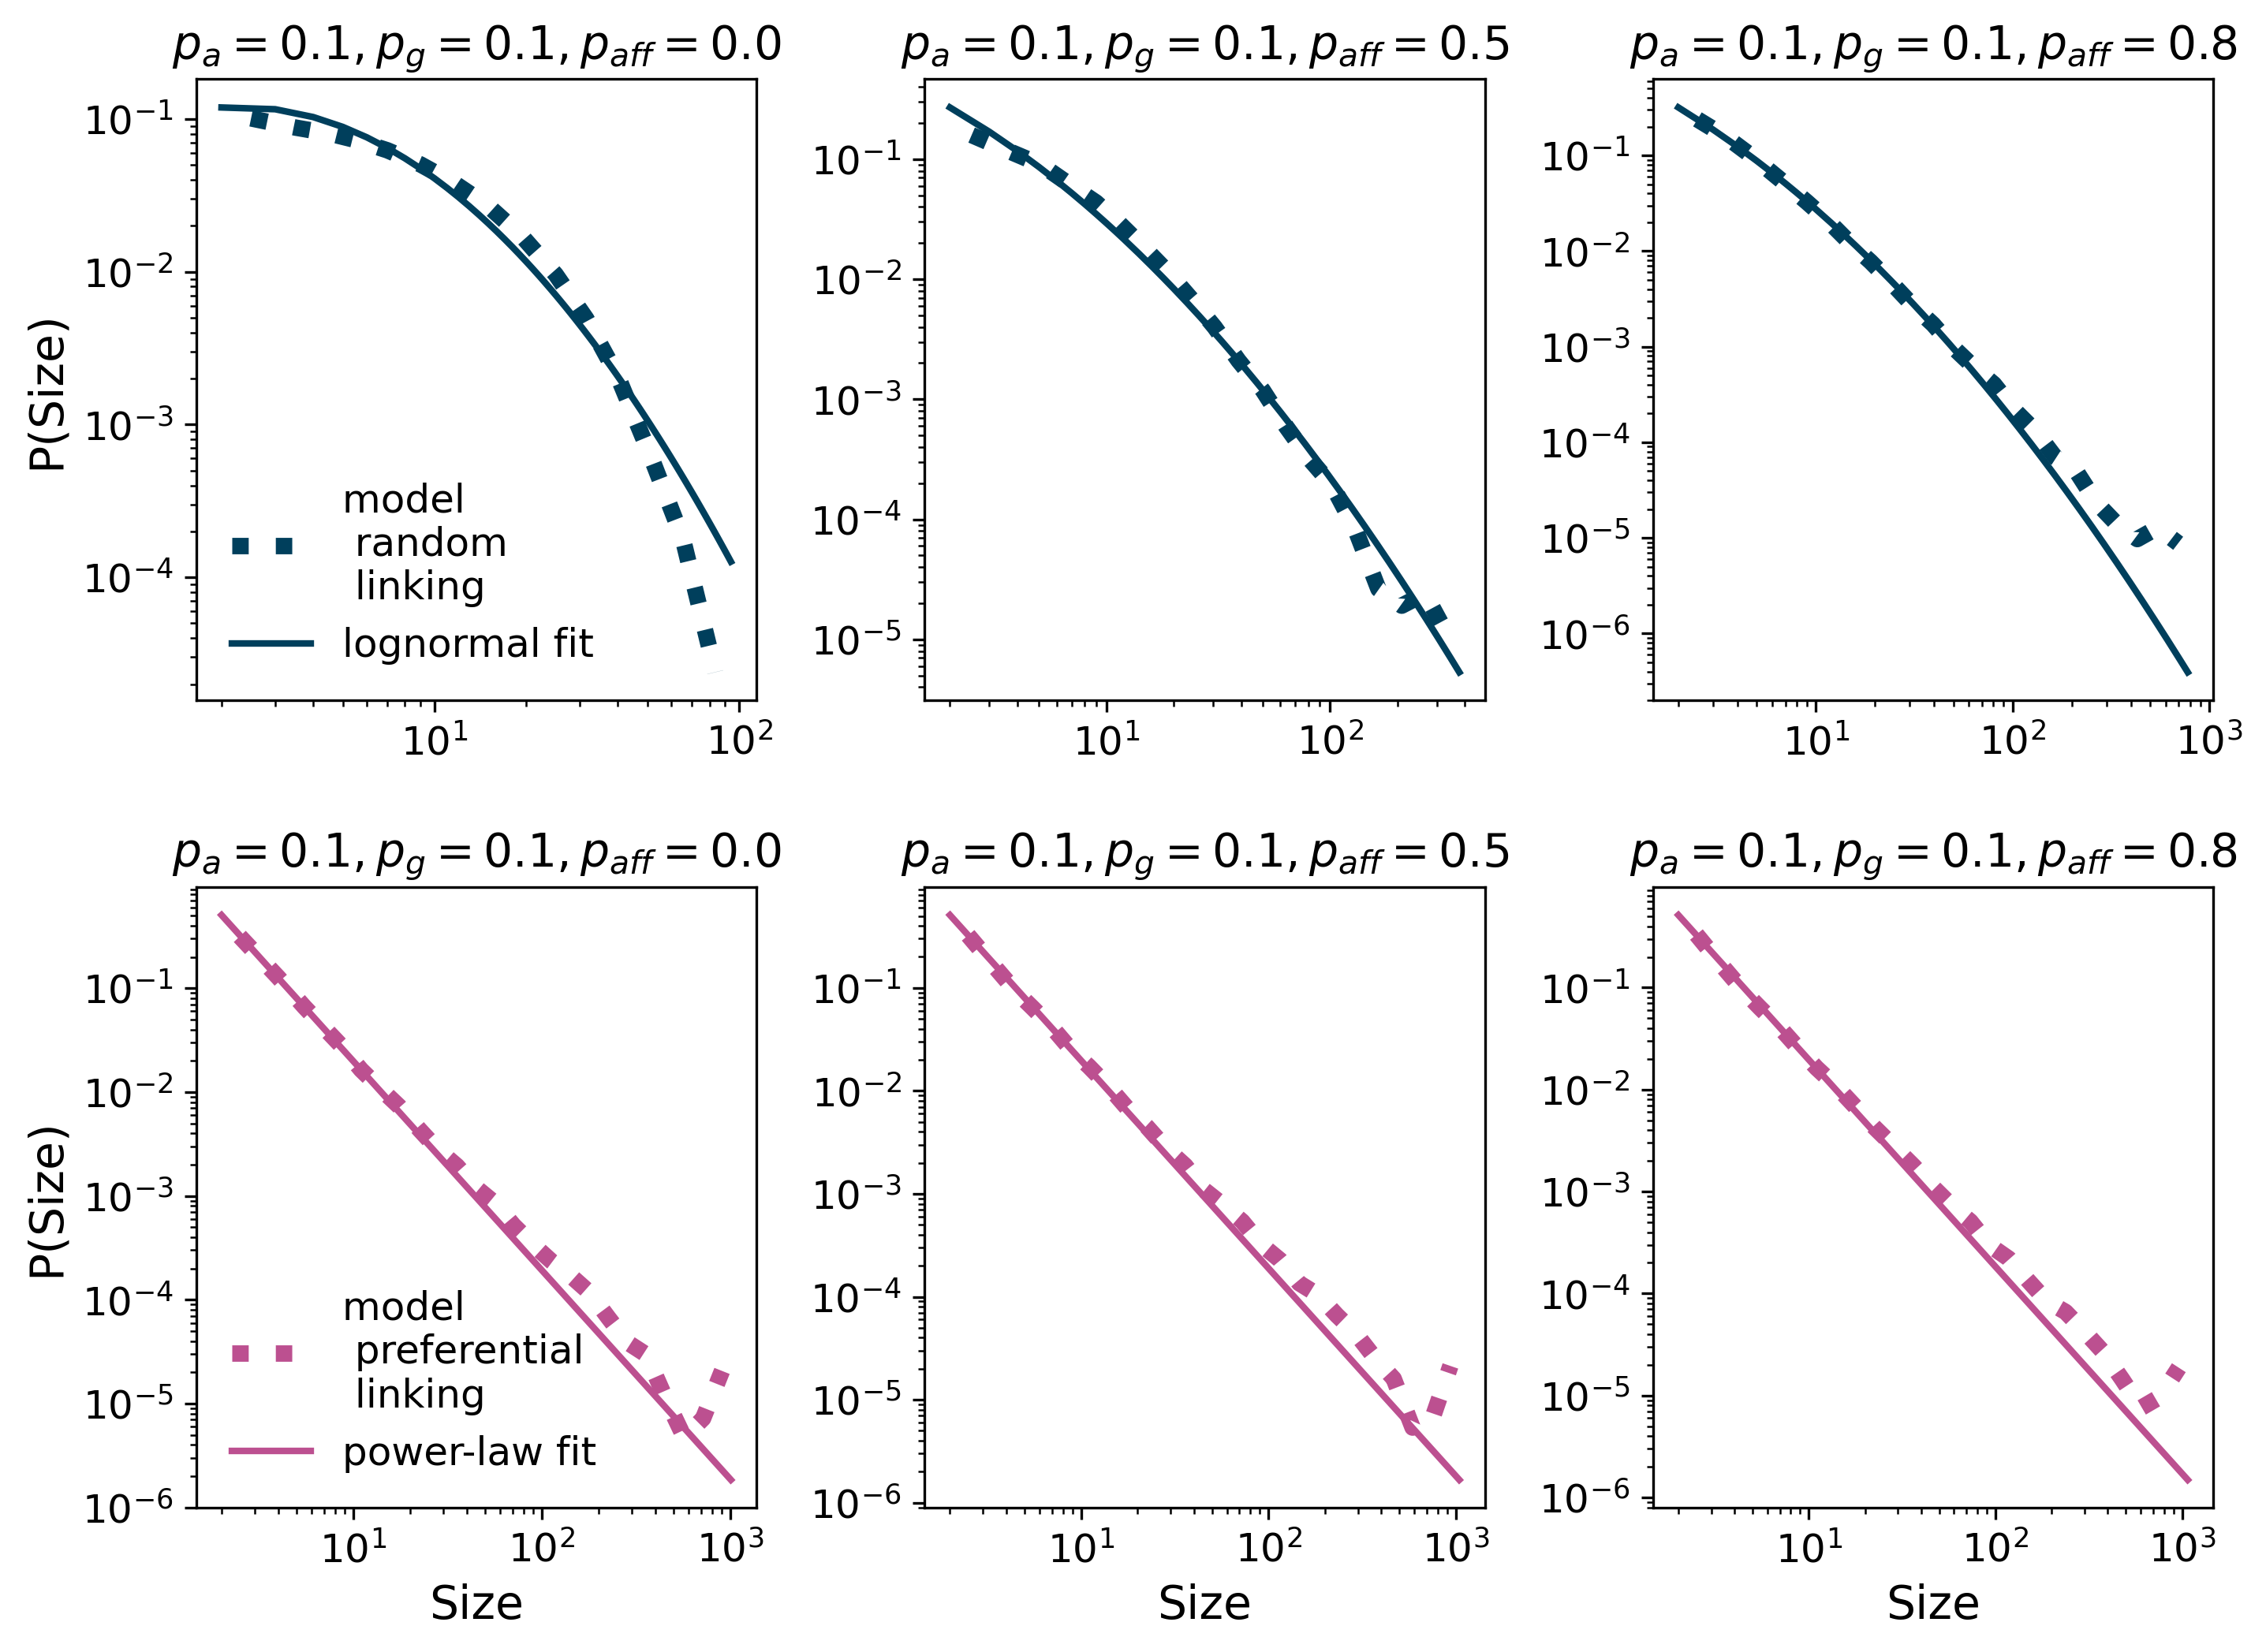
\includegraphics[width=0.7\linewidth]{figures/model_N30.png}
	\caption[Comparison between preferential and random linking in the groups' growth model.]{Groups sizes distributions for groups model, where at each time step the constant number of users arrive, $N=30$ and old users are active with probability $p_a=0.1$. Active users make new groups with probability $p_g=0.1$, while we vary affiliation parameter $p_{aff}$. With probability, $1-p_{aff}$, users choose a group randomly. The group sizes distribution (top row) is described with a lognormal distribution. The distribution has a larger width with a higher affiliation parameter, $p_{aff}$. The bottom row presents the case where with probability $1-p_{aff}$, users prefer larger groups. For all values of parameter $p_{aff}$, we find the power-law group sizes distribution.}
	\label{fig:model_comp}
\end{figure}


%How members are distributed in these groups depends on the parameter $p_{aff}$ value. When $p_{aff}=0$, social connections are irrelevant to the group's choice, and members choose groups randomly. The obtained distribution slightly deviates from lognormal, especially for large group sizes. In this case, large group sizes become more probable than in the case of the lognormal distribution. The non-zero parameter $p_{aff}$ means that the group's choice becomes dependent on social connections. 

%When a member chooses a group according to her social connections, larger groups have a higher probability of being affiliated with the social connections of active members, and thus this choice resembles preferential attachment. For these reasons, the obtained size distribution has more broad tail than the lognormal distribution and begins to resemble power-law distribution.

%The differences between our and the co-evolution model, described in previous sections, at first glance, may appear small. However, they lead to huge differences in the distribution of the size of social groups. The distribution of group sizes in the co-evolution model is a power law. Our model adds flexibility to produce groups with a lognormal size distribution, expanding classes of social systems that can be modelled. 
%Our model is more flexible and can produce groups with lognormal size distribution that better describes diverse social systems, including ones described in Section \ref{sec:emp}.\\
\newpage
\section{Results}

The social systems do not grow at a constant rate. In Ref. \cite{vranic2021growth}, authors have shown that features of growth signal influence the structure of social networks. For these reasons, we use the real growth signal from Meetup groups located in London and New York and Reddit community to simulate the growth of the social groups in these systems. Figure \ref{fig:fig5} top panel shows the time series of the number of new members that join each of the three systems each month. All three systems have relatively low growth initially, which accelerates as the system becomes more popular.

\begin{figure}[h]
	\centering
	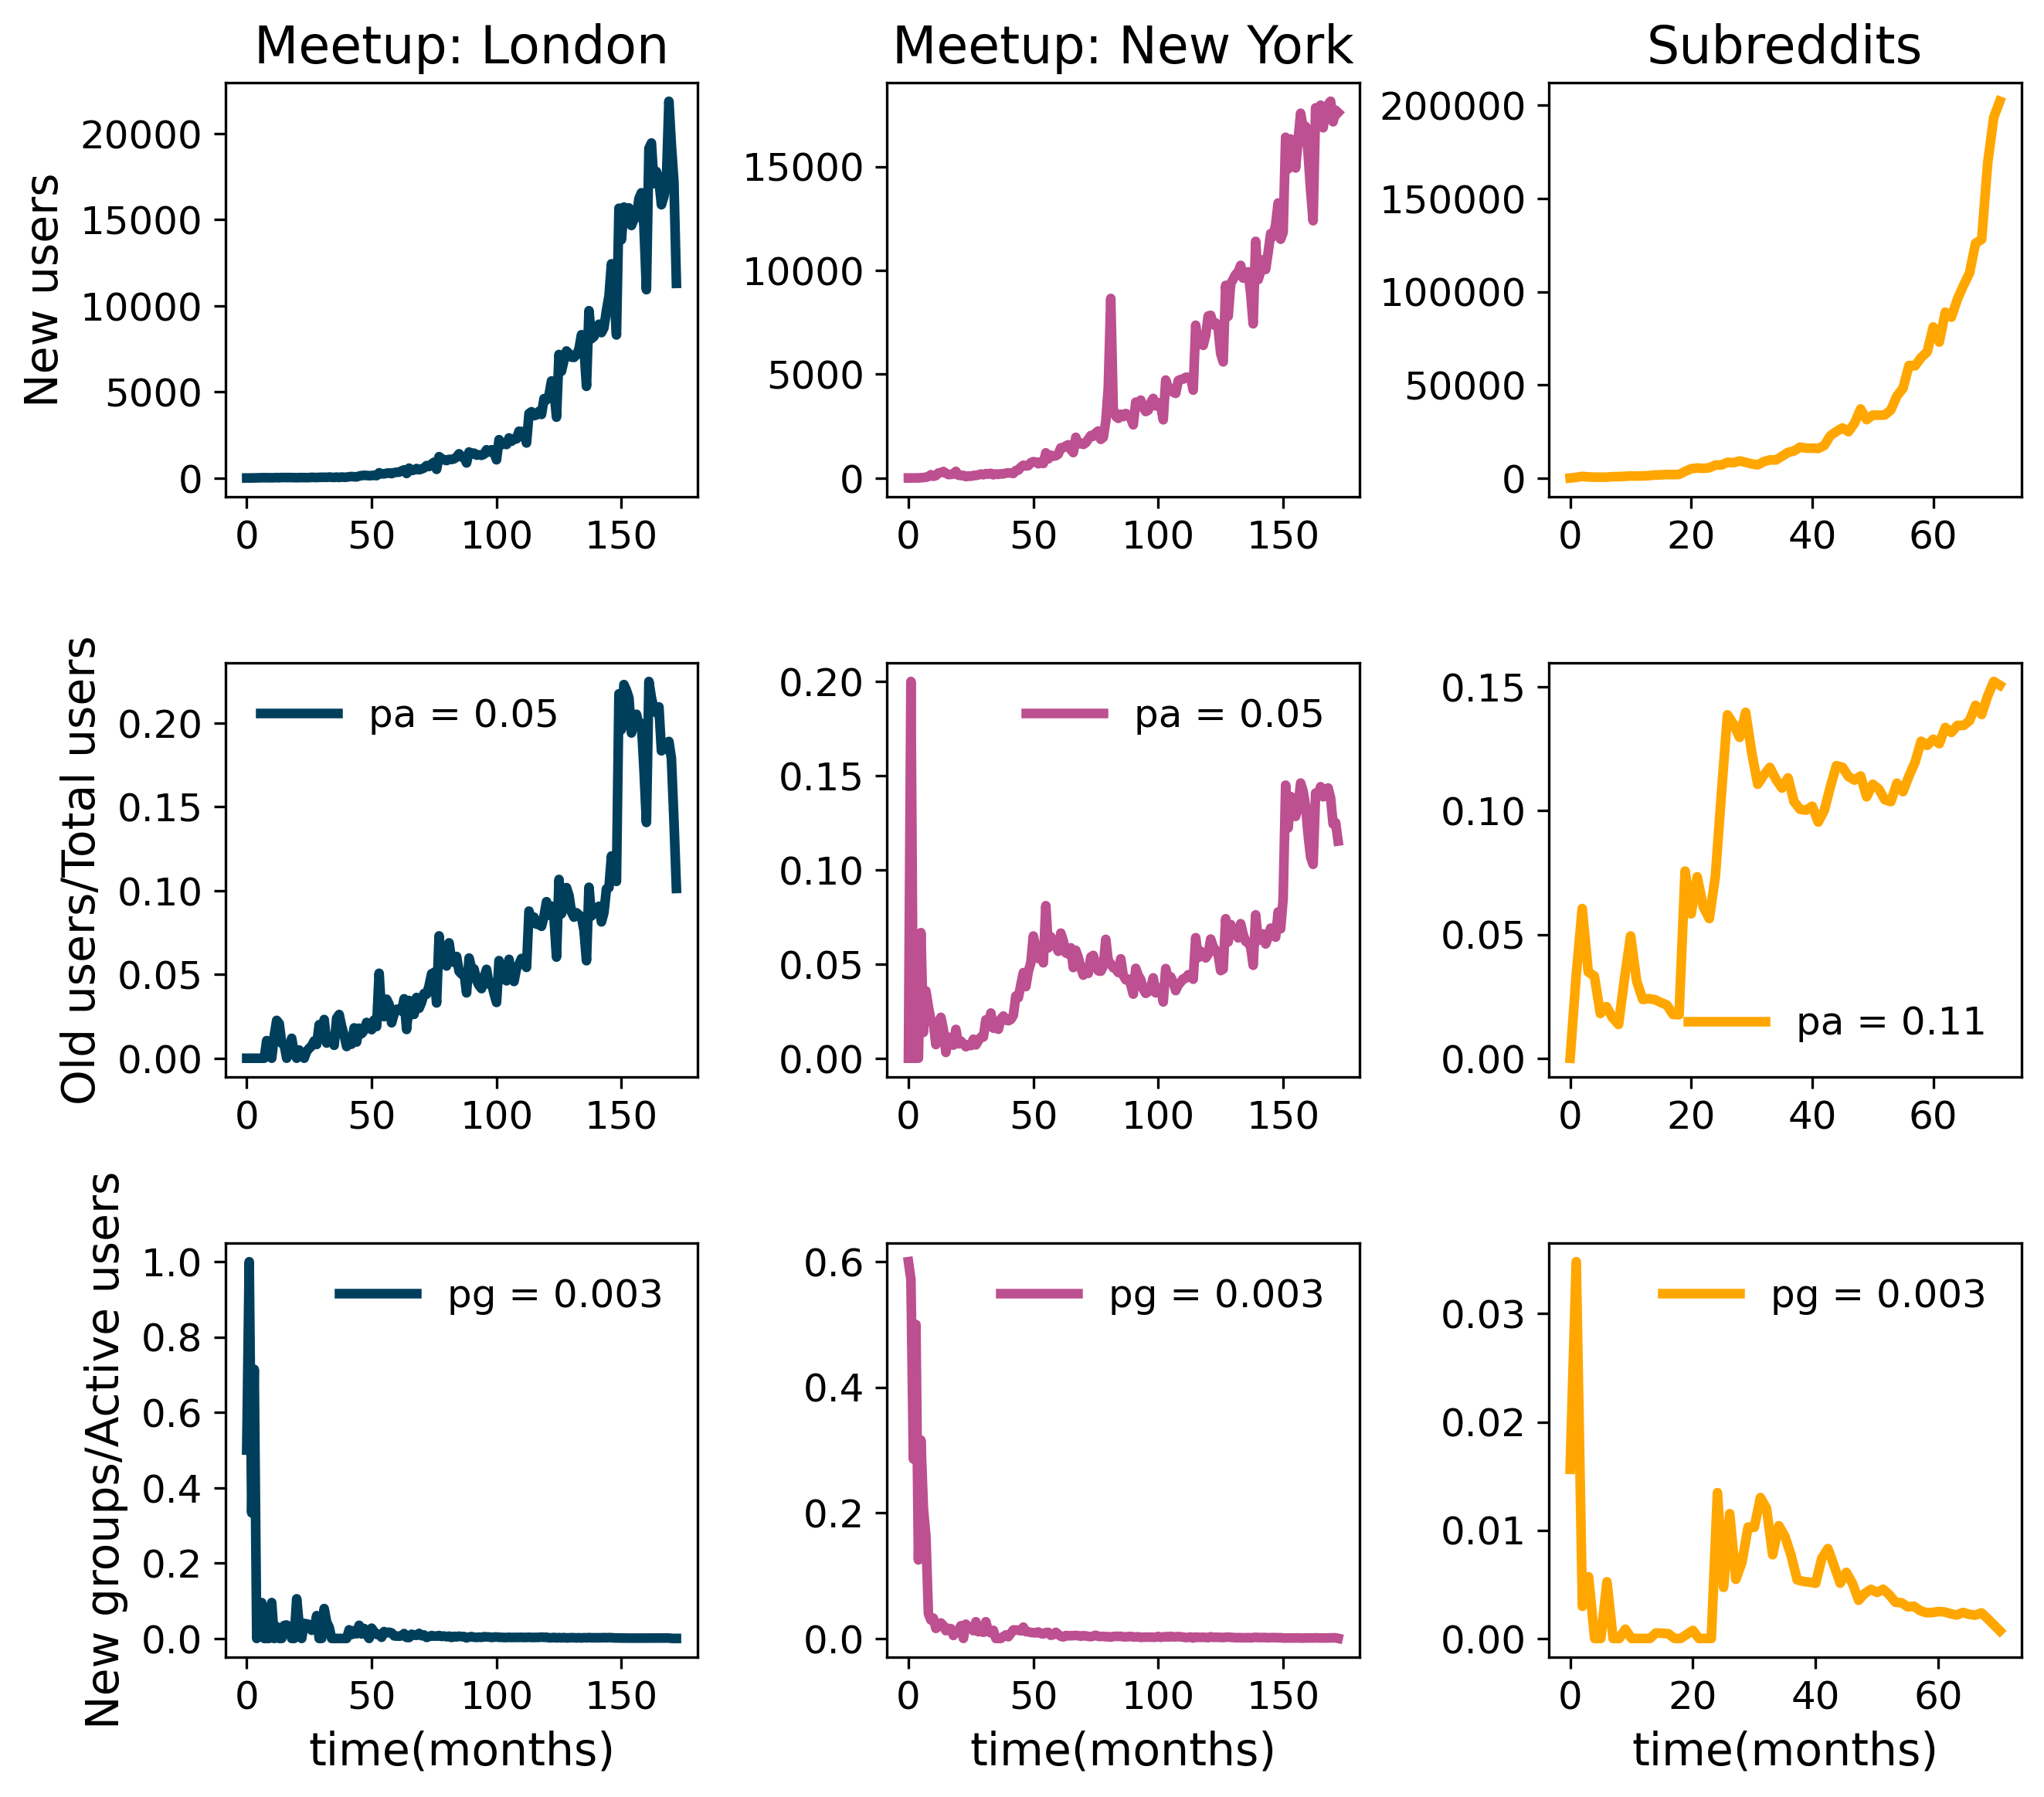
\includegraphics[width=0.7\linewidth]{Figures/figures/Fig3.png}
	\caption[The estimation of the model parameters for a groups growth model.]{The time series of the number of new members (top panel), the ratio between old members and total members in the system (middle panel), and the ratio between new groups and active members(bottom panel) for Meetup groups in London,  Meetup groups in New York, and subreddits. }
	\label{fig:fig5}
\end{figure}

We also use empirical data to estimate $p_{a}$, $p_{g}$ and $p_{aff}$. Probabilities that old members are active $p_a$ and that new groups are created $p_g$ can be approximated directly from the data. Activity parameter $p_{a}$ is the ratio between the number of old members active in month $t$ and the total number of members in the system at time $t$. Figure \ref{fig:fig5} middle row shows the variation of parameter $p_{a}$ during the considered time interval for each system. The values of this parameter fluctuate between $0$ and $0.2$ for London, and New York-based Meetup groups, while for Reddit, it ranges between $0$ and $0.15$.
To simplify our simulations, we assume that $p_{a}$ is constant in time and estimate its value as its median value during the $170$ months for Meetup systems and $80$ months of the Reddit system. For Meetup groups based in London and New York, $p_{a}=0.05$, while Reddit members are more active on average, and $p_{a}=0.11$ for this system.

Figure \ref{fig:fig5} bottom row shows the evolution of parameter $p_{g}$ for the three considered systems. The $p_{g}$ in month $t$ is estimated as the ratio between the groups created in month $t$ $Ng_{new}(t)$ and the total number of groups that month $Ng_{new}(t)+Ng_{old}(t)$, i.e., $p_{g}(t)=\frac{Ng_{new}(t)}{N_{new}(t)+N_{old}(t)}$. We see from Fig. \ref{fig:fig5} that $p_{g}(t)$ has relatively high values at the beginning of the system's existence. In the beginning, these systems have a relatively small number of groups and often cannot meet the needs for the content of all their members. As time passes, the number of groups and content offerings within the system grows, and members no longer have a high need to create new groups. Figure \ref{fig:fig5} shows that $p_{g}$ fluctuates less after the first few months, and thus we again assume that $p_{g}$ is constant in time and set its value to median value during 170 months for Meetup and 80 months for Reddit. For all three systems, $p_{g}$ has the value of $0.003$.



The affiliation parameter $p_{aff}$ cannot estimate directly from the empirical data. For these reasons, we simulate the growth of social groups in each of the three systems with the time series of new members obtained from the real data and estimated values of parameters $p_a$ and $p_g$, while we vary the value of $p_{aff}$. For each of the three systems, we compare the distribution of group sizes obtained from simulations for different values of $p_{aff}$ with ones obtained from empirical analysis using Jensen Shannon (JS) divergence. The JS divergence \cite{jsdivergence} between two distributions $P$ and $Q$ is defined as 
\begin{equation}
JS(P, Q) = H\left(\frac{P+Q}{2}\right) - \frac{1}{2}\left(H(P)+H(Q)\right) \label{eq2}
\end{equation}
where $H(p)$ is Shannon entropy $H(p)=\sum_x p(x)log(p(x)$. The JS divergence is symmetric, and if $P$ is identical to $Q$, $JS=0$. The smaller the JS divergence value, the better the match between empirical and simulated group size distributions. Table \ref{tab:table} shows the value of JS divergence for all three systems. We see that for London-based Meetup groups; the affiliation parameter is $p_{aff}=0.5$, for New York groups $p_{aff}=0.4$, while the affiliation parameter for Reddit $p_{aff}=0.8$. Our results show that social diffusion is important in all three systems. However, Meetup members are more likely to join groups at random, while for Reddit members, their social connections are more important regarding the choice of the subreddit.  


\begin{table}[h]
	\centering
	\begin{tabular}{|c|c|c|c|}
		\hline
		$p_{aff}$ & JS cityLondon   & JS cityNY       & JS reddit2012    \\ \hline
		0.1  & 0.0161          & 0.0097          & 0.00241          \\ \hline
		0.2  & 0.0101          & 0.0053          & 0.00205          \\ \hline
		0.3  & 0.0055          & 0.0026          & 0.00159          \\ \hline
		0.4  & 0.0027          & \textbf{0.0013} & 0.00104          \\ \hline
		0.5  & \textbf{0.0016} & 0.0015          & 0.00074          \\ \hline
		0.6  & 0.0031          & 0.0035          & 0.00048          \\ \hline
		0.7  & 0.0085          & 0.0081          & 0.00039          \\ \hline
		0.8  & 0.0214          & 0.0167          & \textbf{0.00034} \\ \hline
		0.9  & 0.0499          & 0.0331          & 0.00047          \\ \hline
	\end{tabular}
	\caption[Jensen Shannon divergence between group sizes distributions from model and data.]{Jensen Shannon divergence between group sizes distributions from model
		(in the model, we vary affiliation parameter paff) and data.}
	\label{tab:table}
\end{table}

Figure \ref{fig:fig6} compares the empirical and simulation distribution of group sizes for three considered systems. We see that empirical distributions for Meetup groups based in London and New York are perfectly reproduced by the model and chosen values of parameters. In the case of Reddit, the distribution is very broad, and the model well reproduces the tail of the distribution.
The bottom row of Fig. \ref{fig:fig6} shows the distribution of logarithmic values of growth rates of groups obtained from empirical and simulated data. We see that the tails of empirical distributions for all three systems are well emulated by the ones obtained from the model. However, there are deviations which are the most likely consequence of using median values of parameters $p_{a}$, $p_{g}$, and $p_{aff}$.

\begin{figure}[H]
	\centering
	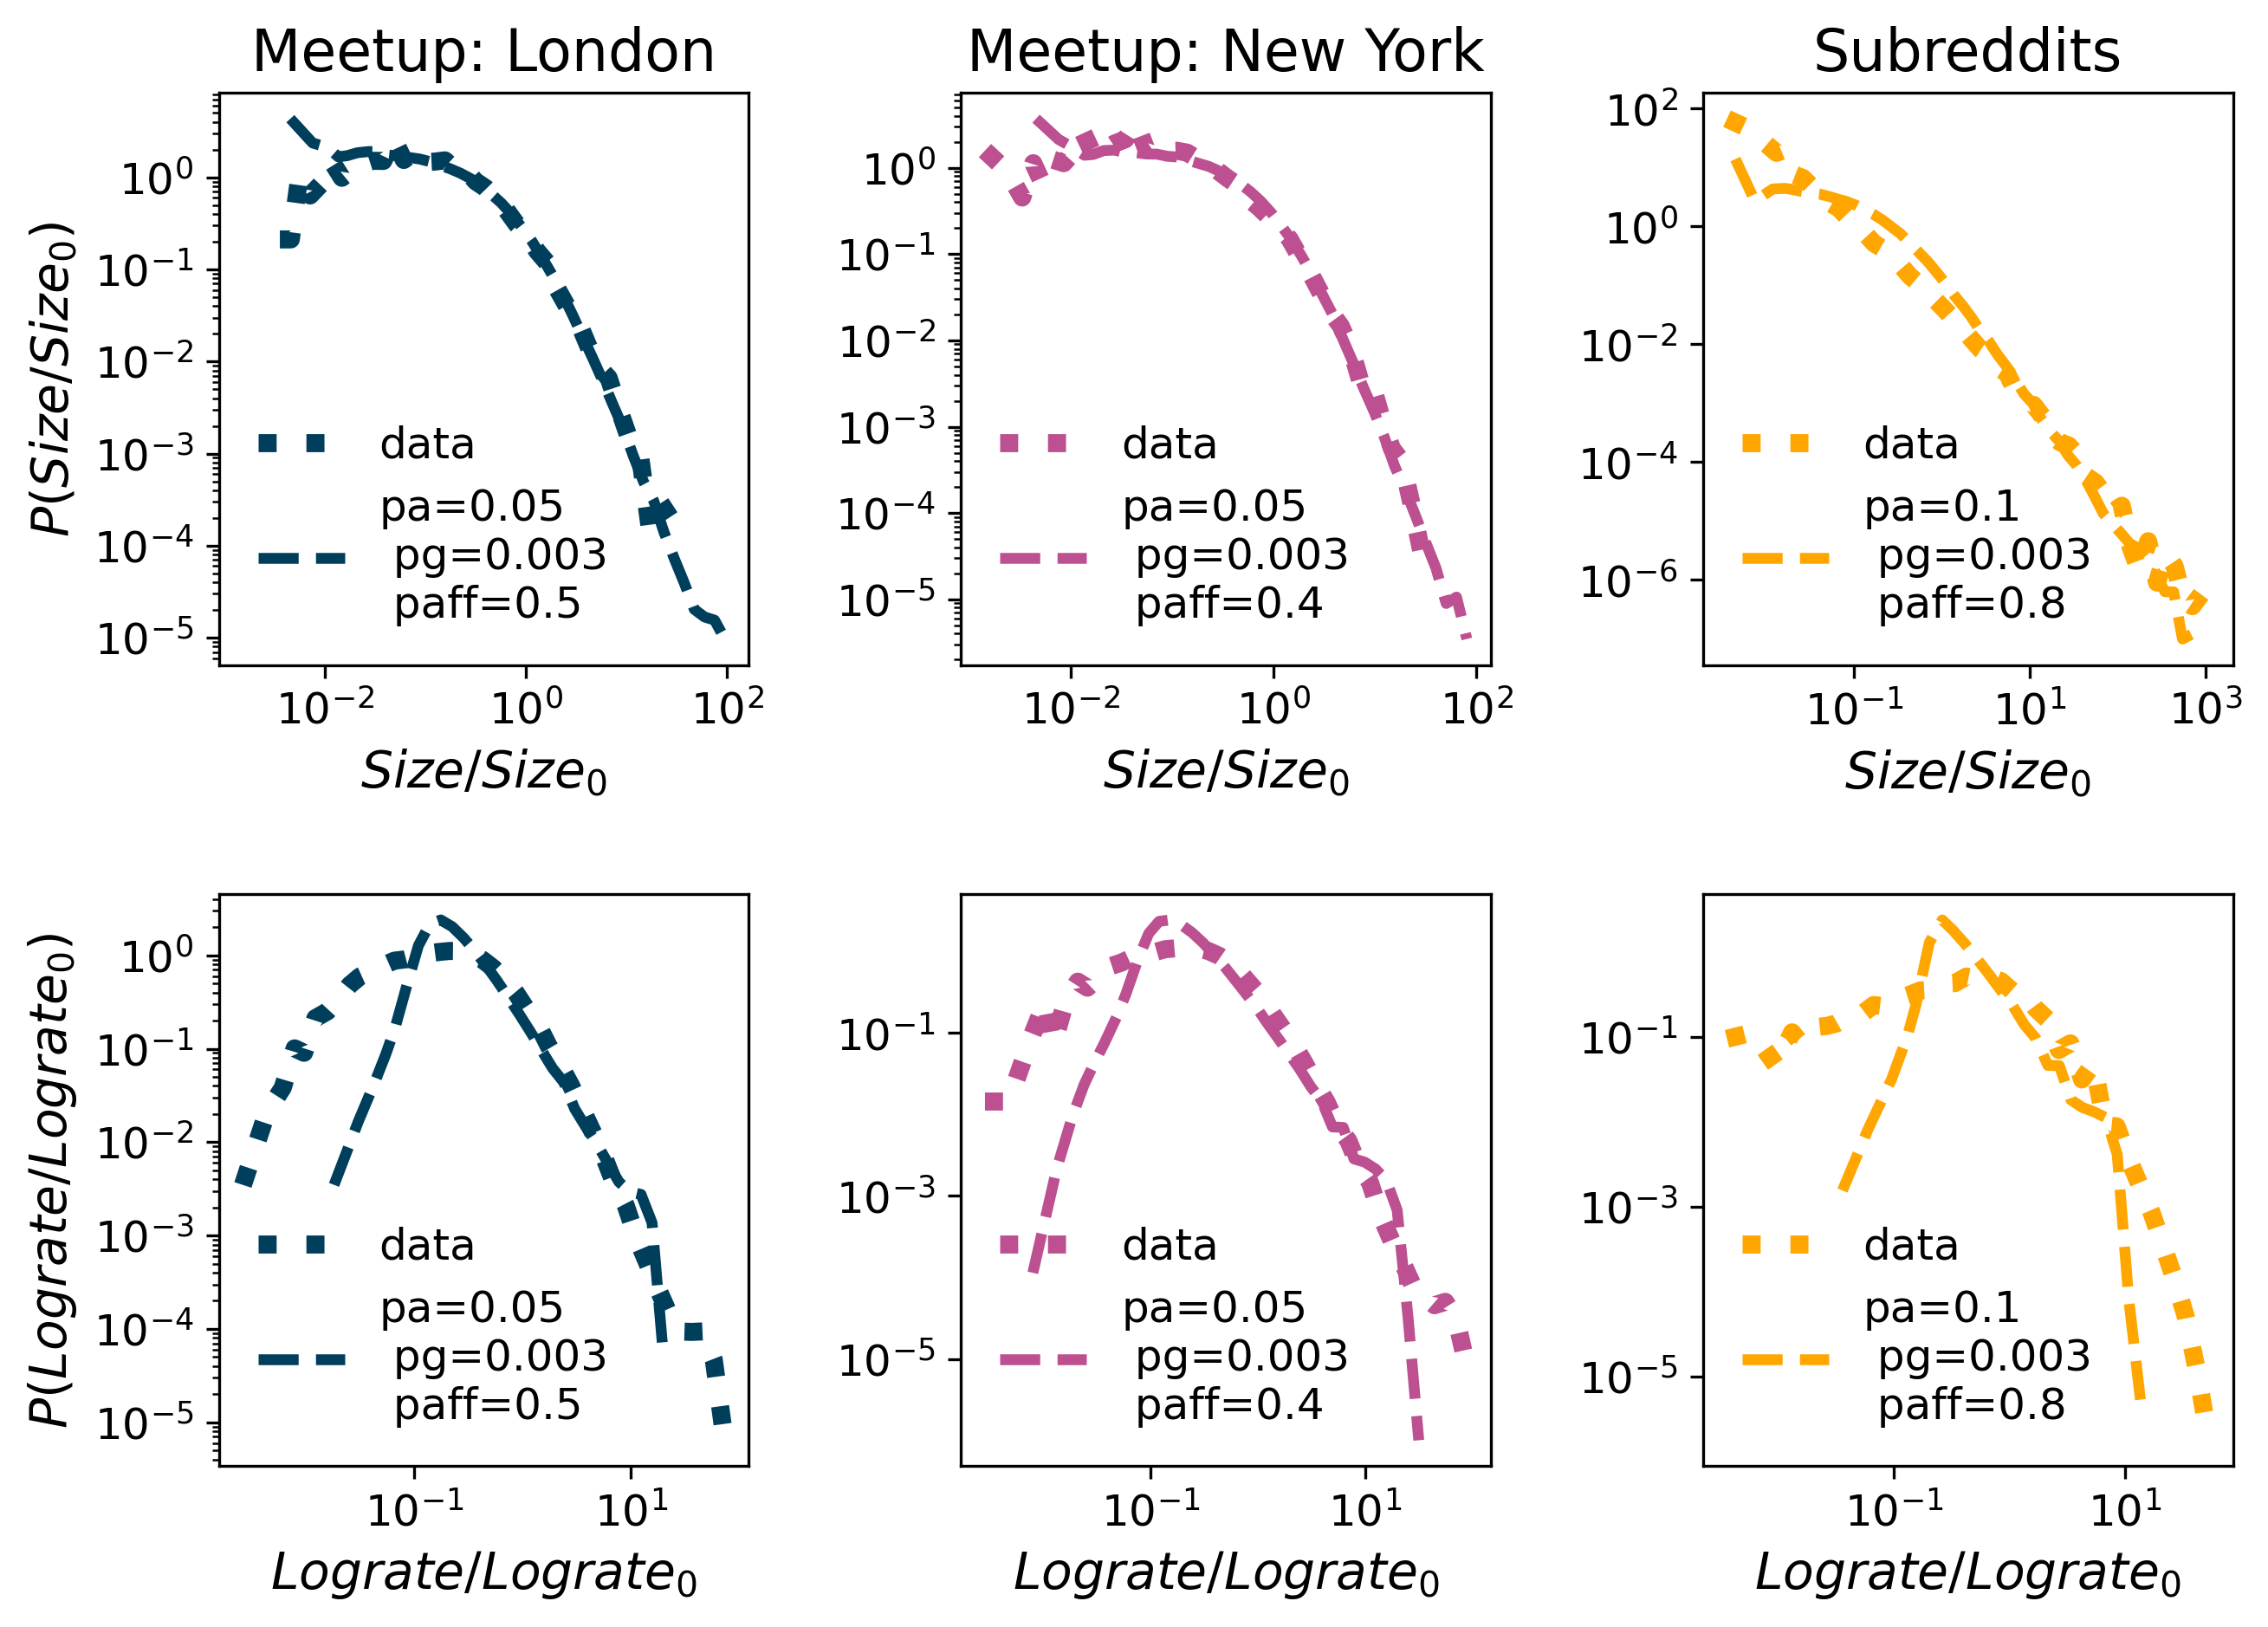
\includegraphics[width=0.8\linewidth]{Figures/figures/Fig4.png}
	\caption[The comparison between empirical and simulated data.]{The comparison between empirical and simulation distribution for group sizes (top panel) and logrates (bottom panel).}
	\label{fig:fig6}
\end{figure}


\subsection{Distributions fit}

We compute the log-likelihood ratio $R$ and $p$-value between different distributions and lognormal fit \cite{clauset2009power} to determine the best fit for the group size distributions. Distribution with a higher likelihood is a better fit. The log-likelihood ratio R has a positive or negative value, indicating which distribution represents a better fit. To choose between two distributions, we need to calculate the p-value to be sure that R is sufficiently positive or negative and that it is not the result of chance fluctuation from the result close to zero. If the p-value is small, $p<0.1$, it is unlikely that the sign of R is the chance of fluctuations, and it is an accurate indicator of which model fits better.

Table \ref{tab:fit-data} summarizes the findings for empirical data on group size distributions from Meetup groups in London and New York, and Reddit. Using the maximum likelihood method, we obtain the parameters of the distributions \cite{power-law}. The results indicate that lognormal distribution best fits all three systems. Figure \ref{fig:fitdata} shows the distributions of empirical data and lognormal fit on data. For Meetup data, we present fit on stretched exponential distribution, which fits a large portion of data well. For subreddits, distribution is broad and potentially resembles power-law. Still, the lognormal distribution is a more suitable fit.

\begin{table}[h]
	\centering
	\caption[The likelihood ratio R and p-value for fitting empirical data]{The likelihood ratio R and p-value between different candidates and \textbf{lognormal} distribution for fitting the distribution of \textbf{groups sizes} of Meetup groups in London, New York and in Reddit. According to these statistics, the lognormal distribution represents the best fit for all communities. \\ }
	\begin{tabular}{|c||cc||cc||cc|}
		\hline
		\multirow{2}{*}{\begin{tabular}[c]{@{}c@{}}distribution \end{tabular}} & \multicolumn{2}{c||}{\begin{tabular}[c]{@{}c@{}}Meetup\\ city London\end{tabular}} & \multicolumn{2}{c||}{\begin{tabular}[c]{@{}c@{}}Meetup\\ city NY\end{tabular}} & \multicolumn{2}{c|}{Reddit}                    \\ \cline{2-7} 
		& \multicolumn{1}{c|}{R}                             & p                            & \multicolumn{1}{c|}{R}                           & p                          & \multicolumn{1}{c|}{R}         & p             \\ \hline \hline \hline
		exponential                                                                            & \multicolumn{1}{c|}{-8.64e2
			%-864.86
		}                       & 8.11e-32                     & \multicolumn{1}{c|}{-8.22e2}                     & 6.63e-26                   & \multicolumn{1}{c|}{-3.85e4} & 1.54e-100     \\ \hline
		\begin{tabular}[c]{@{}c@{}}stretched \\ exponential\end{tabular}                       & \multicolumn{1}{c|}{-3.01e2}                       & 1.00e-30                      & \multicolumn{1}{c|}{-1.47e2}                     & 7.78e-8                    & \multicolumn{1}{c|}{-7.97e1}    & 5.94e-30      \\ \hline
		power law                                                                              & \multicolumn{1}{c|}{-4.88e3}                      & 0.00                         & \multicolumn{1}{c|}{-4.57e3}                    & 0.00                       & \multicolumn{1}{c|}{-9.39e2}   & 4.48e-149 \\ \hline
		\begin{tabular}[c]{@{}c@{}}truncated \\ power law\end{tabular}                         & \multicolumn{1}{c|}{-2.39e3}                      & 0.00                         & \multicolumn{1}{c|}{-2.09e3}                    & 0.00                       & \multicolumn{1}{c|}{-5.51e2}   & 2.42e-56      \\ \hline
	\end{tabular}
	\label{tab:fit-data}
\end{table}

\begin{figure}[ht]
	\centering
	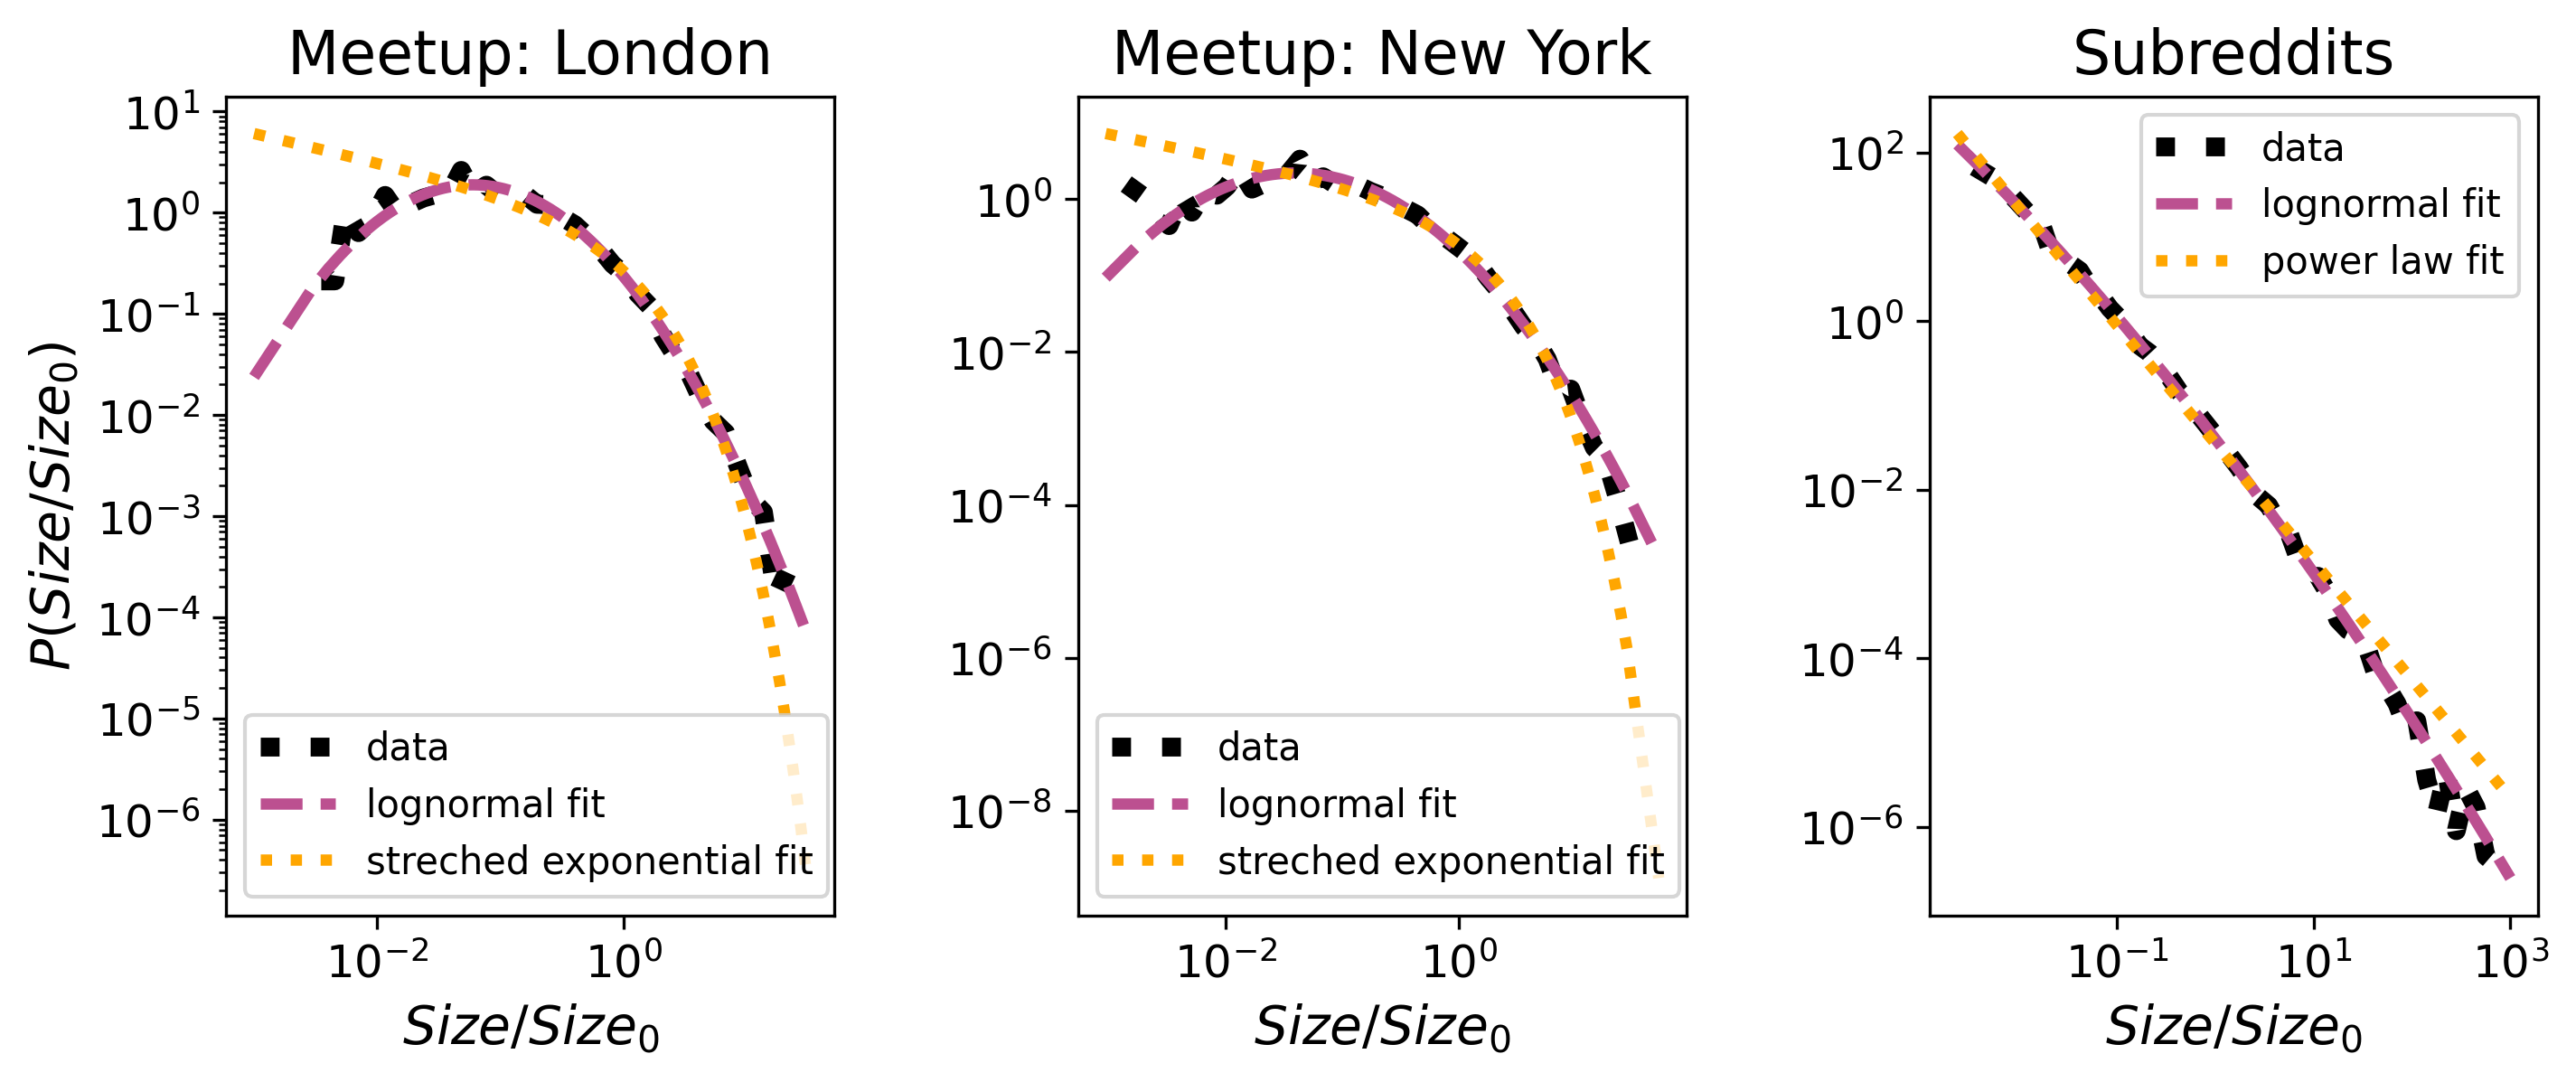
\includegraphics[width=0.8\linewidth]{figures/FigA1_data.png}
	\caption[The fitting of empirical group size distributions.]{The comparison between lognormal and stretched exponential fit to London and NY data,  and between lognormal and power law for Subreddits. The parameters for lognormal fits are 1) for city London $\mu=-0.93$ and $\sigma = 1.38$, 2) for city NY $\mu=-0.99$ and $\sigma = 1.49$, 3) for Subreddits $\mu=-5.41$ and $\sigma = 3.07$.  }
	\label{fig:fitdata}
\end{figure}

We use the same methods to estimate the fit for simulated group size distributions on Meetup groups in London, New York, and Subreddits. Table \ref{tab:fit_model} shows the results of the log-likelihood ratio R and $p$-value between different distributions. We conclude that lognormal distribution is most suitable for simulated group size distributions. We confirm our observations by plotting lognormal and stretched exponential fit on data, Fig. \ref{fig:fit_model}.  
% Please add the following required packages to your document preamble:
% \usepackage{multirow}
\begin{table}[!ht]
	\centering
	\caption[The likelihood ratio R and p-value for fitting simulated data]{The likelihood ratio R and p-value between different candidates and \textbf{lognormal}
		distribution for fitting the distribution of \textbf{simulated group sizes} of Meetup groups in London, New York and Reddit. According to these statistics, the lognormal distribution
		represents the best fit for all communities.}
	\begin{tabular}{|c||cc||cc||cc|}
		\hline
		\multirow{2}{*}{\begin{tabular}[c]{@{}c@{}}distribution \end{tabular}} & \multicolumn{2}{c||}{\begin{tabular}[c]{@{}c@{}}Meetup\\ city London\end{tabular}} & \multicolumn{2}{c||}{\begin{tabular}[c]{@{}c@{}}Meetup\\ city NY\end{tabular}} & \multicolumn{2}{c|}{Reddit}                \\ \cline{2-7} 
		& \multicolumn{1}{c|}{R}                              & p                           & \multicolumn{1}{c|}{R}                            & p                         & \multicolumn{1}{c|}{R}         & p         \\ \hline \hline \hline
		exponential                                                                            & \multicolumn{1}{c|}{-6.27e4}                      & 0.00                        & \multicolumn{1}{c|}{-5.11e4}                    & 0.00                      & \multicolumn{1}{c|}{-1.26e5} & 7.31e-125 \\ \hline
		\begin{tabular}[c]{@{}c@{}}stretched\\ exponential\end{tabular}                        & \multicolumn{1}{c|}{-1.01e4}                      & 1.96e-287                    & \multicolumn{1}{c|}{-6.69e3}                     & 1.46e-93                  & \multicolumn{1}{c|}{-1.39e4} & 0.00      \\ \hline
		power law                                                                              & \multicolumn{1}{c|}{-2.29e5}                     & 0.00                        & \multicolumn{1}{c|}{-3.73e5}                   & 0.00                      & \multicolumn{1}{c|}{-4.38e4} & 0.00      \\ \hline
		\begin{tabular}[c]{@{}c@{}}truncated\\ power law\end{tabular}                          & \multicolumn{1}{c|}{-9.28e4}                      & 0.00                        & \multicolumn{1}{c|}{-1.55e5}                   & 0.00                      & \multicolumn{1}{c|}{-9.12e4} & 0.00      \\ \hline
	\end{tabular}
	\label{tab:fit_model}
\end{table}
\clearpage
\newpage
%\clearpage
\begin{figure}[H]
	\centering
	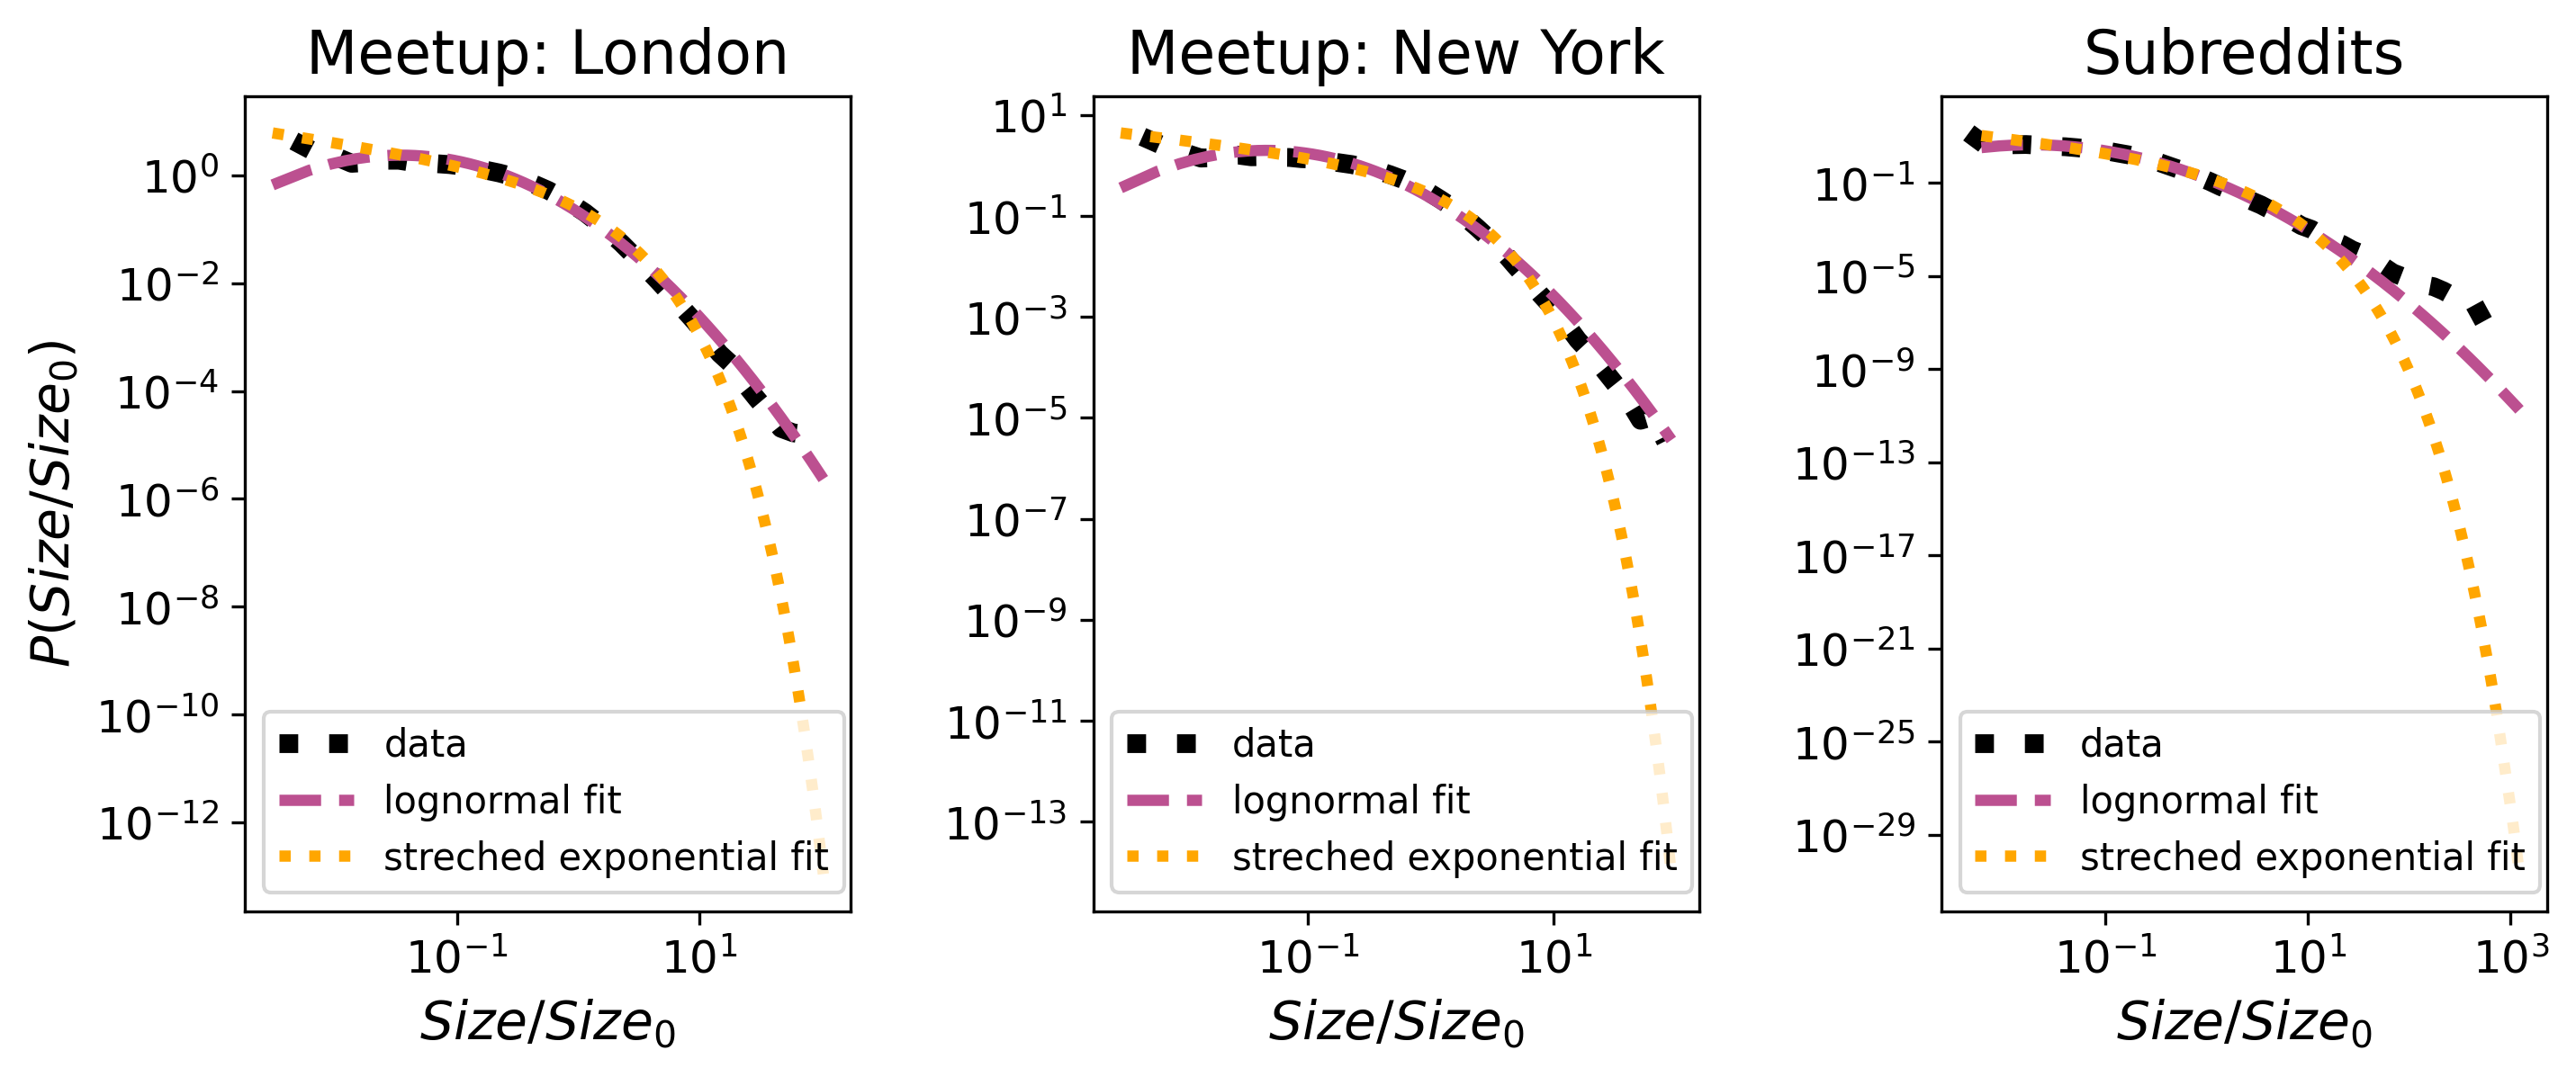
\includegraphics[width=0.8\linewidth]{figures/FigA2-model.png}
	\caption[The fitting of simulated group size distributions.]{The comparison between lognormal and stretched exponential fit to simulated group size distributions. The parameters for lognormal fits are 1) for city London $\mu=-0.97$ and $\sigma = 1.43$, 2) for city NY $\mu=-0.84$ and $\sigma = 1.38$, 3) for Subreddits $\mu=-1.63$ and $\sigma = 1.53$. }
	\label{fig:fit_model}
\end{figure}


\subsection{Users partition in bipartite network - degree distribution}

So far, the group growth model has focused on the degree distribution of groups and under what rules the universalities in the system reflected in the lognormal distribution of group sizes emerge. The model parameter $p_a$ controls the users' activity level; otherwise, it shapes the degree distribution of users in the bipartite network. As this probability is constant and uniform among all users, we do not expect rich properties of users' degree distribution. The expected distribution is exponential for growing random graph \cite{barabasi1999mean}, and the groups' growth model produces the same property. In figure \ref{fig:users_degree}, blue dots show degree distributions of modelled Meetup and Reddit systems. This distribution is very well fitted with exponential form.
Furthermore, in empirical data, these distributions are long-tailed, green dots in figure \ref{fig:users_degree}, so the model can not reproduce the degree distribution of the users. In real systems, the probability that the user is active does not have to be uniform and constant. The previous work proposed that each user has a specific lifetime \cite{leskovec2008microscopic}, but different linking rules could play an important role in shaping users' degree distribution. For example, $p_a$ could be preferential toward high-degree users or even be time-dependent.

\begin{figure}[h]
	\centering
	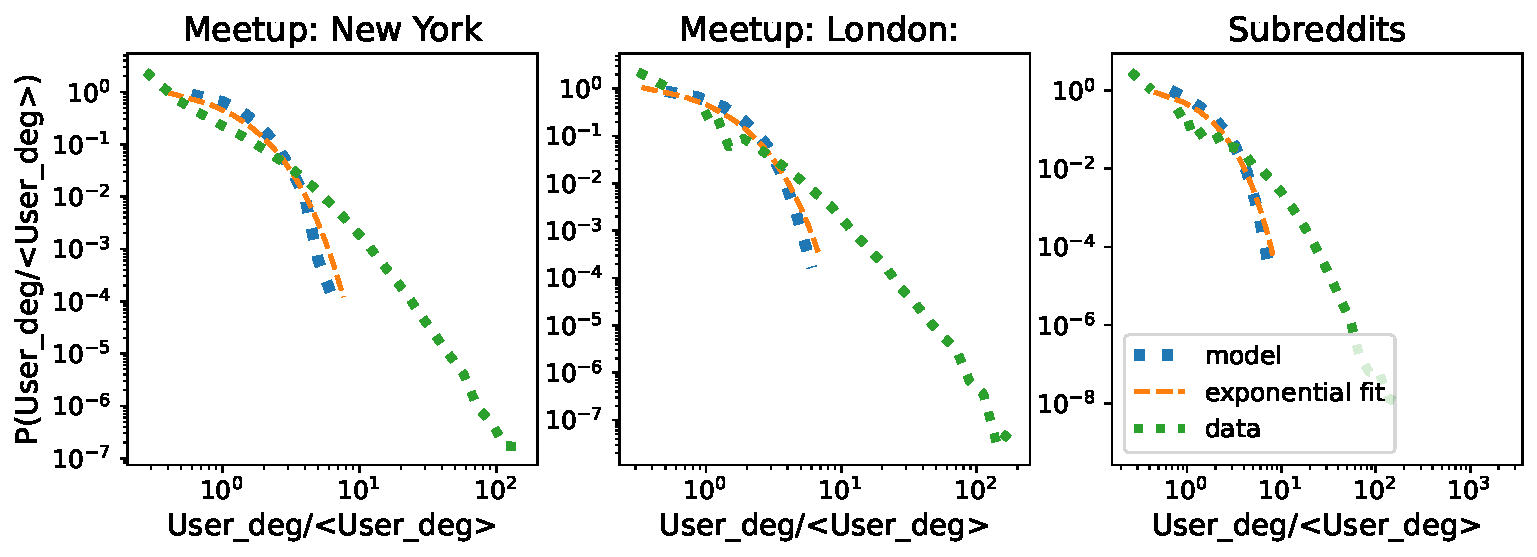
\includegraphics[width=1\linewidth]{groups/users_degree_expfit.pdf}
	\caption[Users degree distribution]{Users degree distribution}
	\label{fig:users_degree}
\end{figure}

\newpage
\section{Conclusions}

We apply complex network theory and statistical physics methods to describe the evolution of online social groups, Meetups in London and NewYork and Reddits. Instead of studying user interaction networks in a single group, which is a common approach, we are interested in quantifying how users interact with the system of multiple groups and determining which processes drive the growth of groups. Similar systems have been analyzed before. For example, it was found that the distribution of the cities or firms follows the lognormal and stays stable, showing universal behaviour. Contrary, the previous work on online social groups indicated that group size distributions of LiveJournal and Youtube follow power-law \cite{zheleva2009co}. On the other hand, for Meetup and Reddit, we find the emergence of lognormal distribution of group sizes, and the distribution of Reddit is much broader. Furthermore, these systems grow exponentially in the number of groups and new users. 

Meetup and Reddit may be platforms with different purposes, but on the lower level, both systems could be described with the same processes users perform: they can join existing groups or create new ones. Also, in these systems, new users constantly arrive. As we find the lognormal distribution in group sizes, our first attempt was to describe this system with the Gibrat model. It is a proportional growth size model, where group size distribution converges to the lognormal distribution while the log rates take the normal distribution. The second condition still needs to be met, so we need to use a more intricate method.

To explore the growth of these systems in more detail, we use a model where the social system is presented with evolving bipartite and social networks \cite{zheleva2009co}. The bipartite network has partitions of users and groups, and a link exists if a user is a group member. The social network describes the social connections between members. At each time step, new users arrive in the system, following the time series of new users, and with probability, $p_a$ old members decide to be also active. The active users can create a new group with probability $p_g$; otherwise, they will join existing groups. Their decision to select a group based on social connection is determined with probability $p_{aff}$; otherwise, the choice is random. 

We estimate model parameters $p_a$, $p_g$ and $p_{aff}$ from empirical data. We see that model approximates well the empirical distributions. For Meetup groups in London and New York, the $p_{aff}$ parameter is smaller, while for Reddit, $p_{aff}$ is higher, resulting in broader group size distribution. It also means that for Reddit members, social connections are more important for the choice of groups. 

With results in this chapter, we contribute to the knowledge of the growth and segmentation of the socio-economic systems. Our work was motivated by the Co-evolution model \cite{zheleva2009co}. The authors explore the social groups in which group size distribution scales as power-law. We identified different universality class, the system where group size distribution follows log normal. Further, we marked off a set of linking rules which led to lognormal group size distribution and compared these two cases. By this, we expanded the classes of social systems that can be modelled.  










%
\chapter{The sustainability of evolving knowledge-based communities} % Main chapter title
\label{Ch:Trust}
%%TODO The sustainability of evolving knowledge-based communities

The \textbf{Stack Exchange} (SE) is a network of question-answer websites on diverse topics. In the beginning, the focus was on computer programming questions with StackOverflow \footnote{
	More information about StackOverflow is available at \url{https://stackoverflow.co/}, and a broad introduction to the SE network is available at: \url{https://stackexchange.com/tour}. 
}  community. Its popularity led to the Stack Exchange network, which counts more than 100 communities on different topics. The SE communities are self-moderating, and the questions and answers can be voted, allowing users to earn Stack Exchange reputation and privileges on the site. %TODO nedostaje pasus da opise vezu izmedju odrzivosti, evolucije istrukture mreze

The new site topics are proposed through site Area51 \footnote{Visit \url{https://area51.stackexchange.com/faq} for more details about closed and beta SE communities and the review process.}, and if the community finds them relevant, they are created. Every proposed  StackExchange site needs interested users to commit to the community and contribute by posting questions, answers and comments. After a successful private beta phase site reaches the public beta phase, other members can join the community. The site can be in the public beta phase for a long time until it meets specific SE evaluation criteria for graduation. Otherwise, it may be closed with a decline in users’ activity. However, SE criteria for graduation have not been applied consistently on every SE site, as many sites graduated without reaching all required thresholds. As those measures only quantify the overall number of questions, answers or highly active users, we want to understand how SE community structure evolves and identify factors that influence sustainability. The need to share knowledge with others motivates users to use Q-A platforms. Still, the fact that they interact with each other reveals their sense of belonging to the community and the presence of trust among users. Our proxy for measuring trust in the community is the Dynamic Interaction Based Reputation Model.

We focused analysis on four pairs of SE communities with the same topic. Astronomy, Literature and Economics are active communities \footnote{Astronomy, Literature and Economics graduated on December 2021 and during our research, they were still in the public beta phase.} The first time, these communities were unsuccessful and thus closed. We also compare closed Theoretical Physics with the Physics site, considering that those two topics engage the similar type of users. 

\section{Network properties of Stack Exchange data}

On Stack Exchange sites, the interaction between users happens through posts. As we are interested in examining the characteristics of the users, we map interaction data to the networks. Using complex network theory, we can quantify the properties of obtained networks and compare different SE communities, e.g. alive and closed SE sites. 

In the user interaction network, the link between two nodes, user $i$ and $j$, exists if user $i$ answers or comments on the question posted by user $j$ or user $i$ comments on the answer posted by user $j$. The created network is undirected and unweighted, meaning that we do not consider multiple interactions between users or the direction of the interaction. 

The first approach is to aggregate all interactions in the first 180 days and study the properties of the static network. Many local and global network measures are dependent 
\cite{boccaletti2006complex}, and it was shown that degree distribution, degree-degree correlations and clustering coefficient are sufficient for the description of the properties of complex networks \cite{orsini2015quantifying}. 

We calculate the \textbf{degree distribution}, Figure \ref{fig:fullnetdeg}, and compare the distributions of active and closed communities of the same topic. Degree distributions between active and closed communities follow similar lines. 

\begin{figure}[ht]
	\centering
	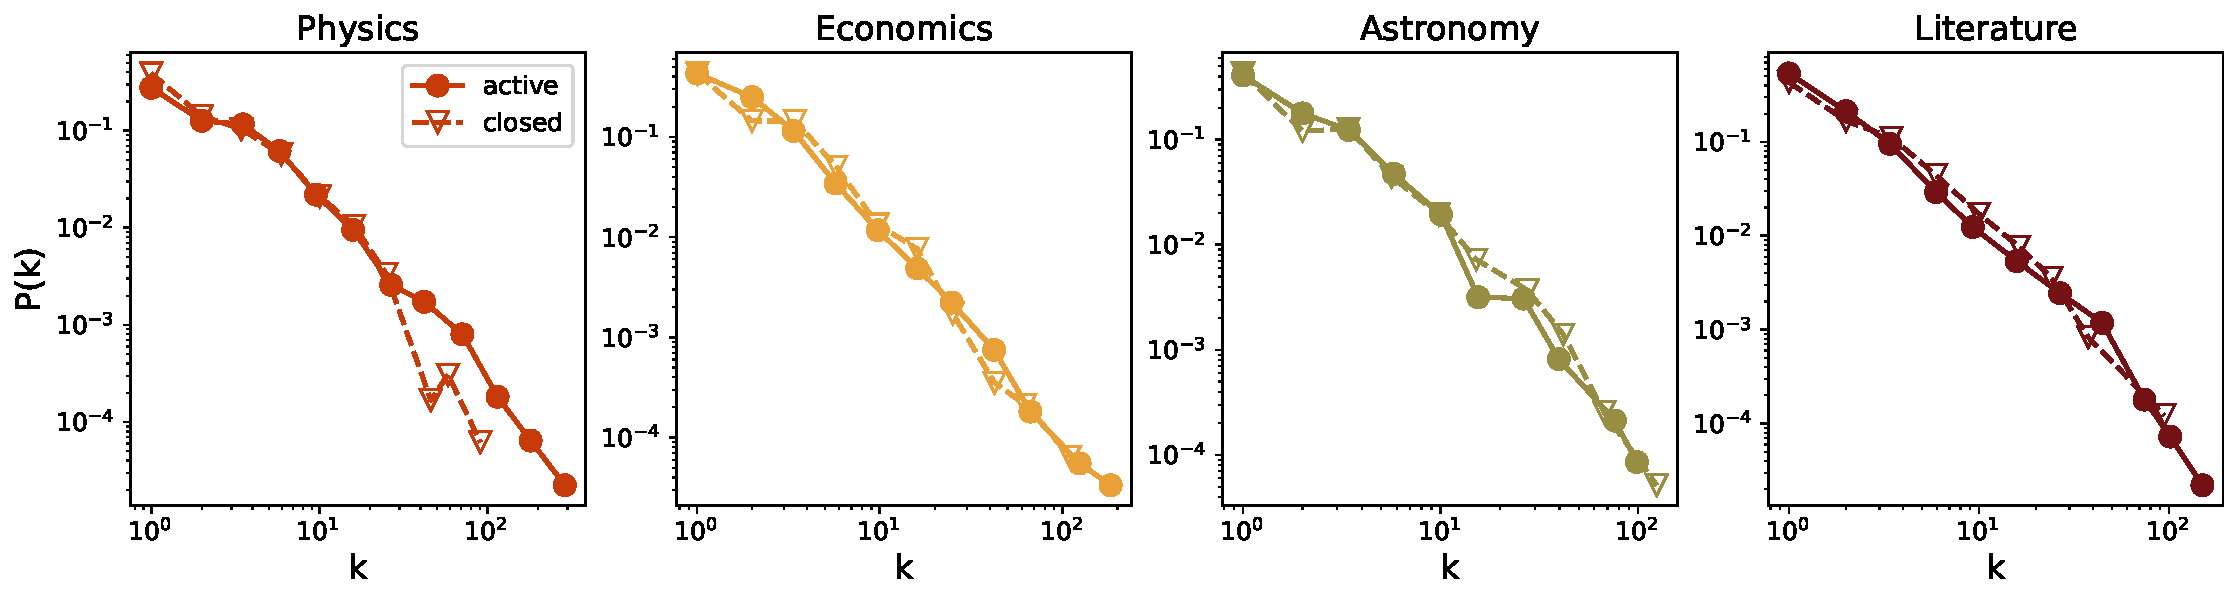
\includegraphics[width=\linewidth]{chapter5/degree_distribution_fullnet.pdf}
	\caption{Degree distribution.}
	\label{fig:fullnetdeg}
\end{figure}

If we take a look into \textbf{neighbor degree} depending on the node degree $k_{nn}(k)$, Figure \ref{fig:fullneighdeg}, we find that there are structural differences between networks formed in the active and closed communities. On average, $k$-degree users in active communities have neighbours with a larger degree than is the case in closed communities. The results are consistent for Physics, Economics and Literature. For Astronomy, we find different behaviour, where the $k_{nn}(k)$ distributions of closed communities are on top of the distributions of the active ones. 

\begin{figure}[!ht]
	\centering
	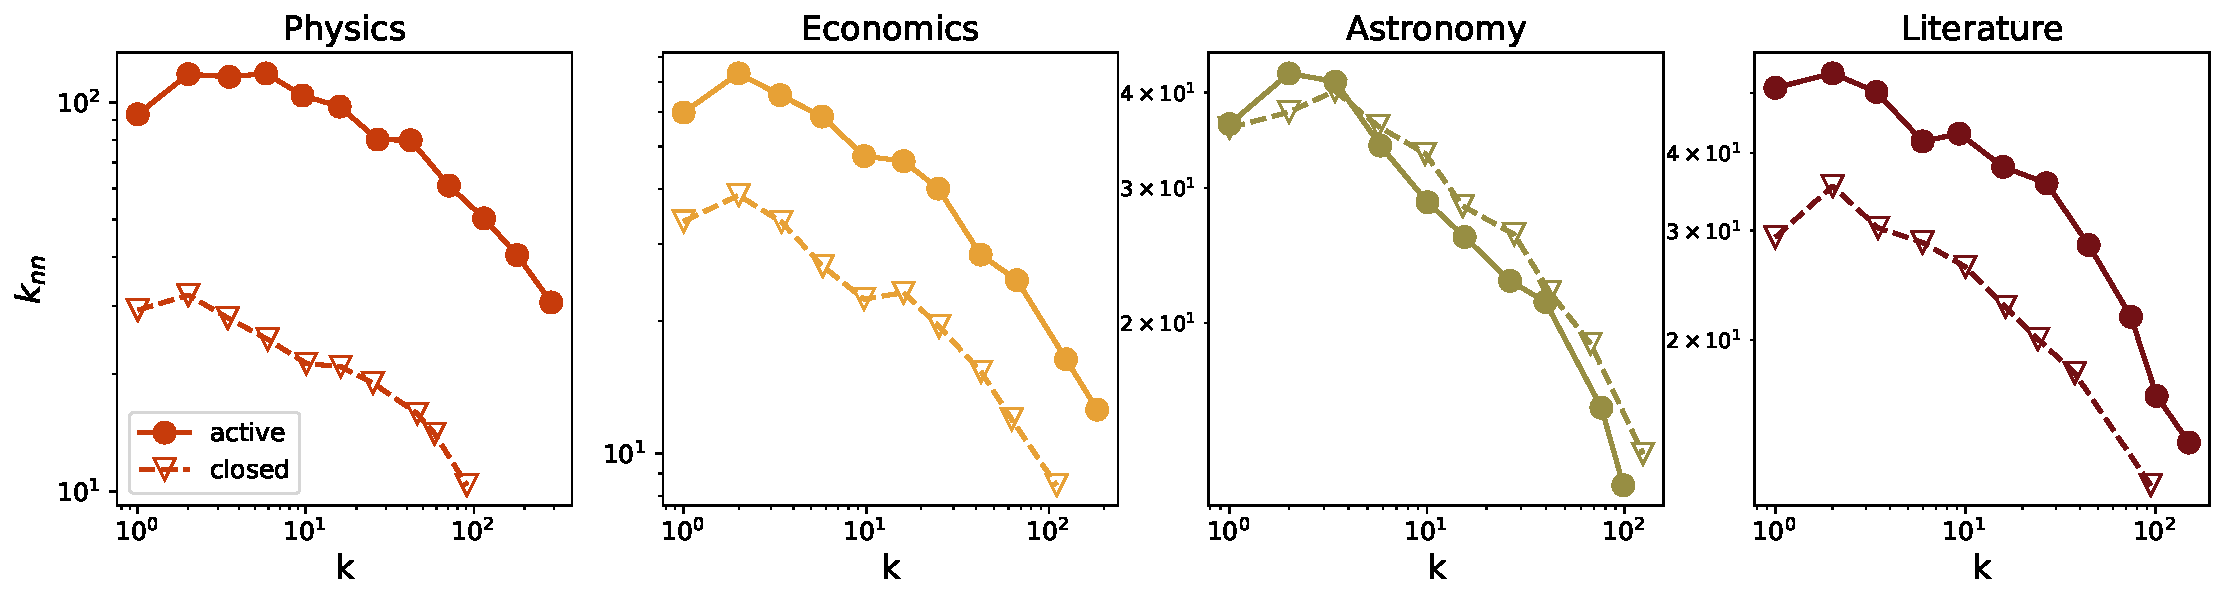
\includegraphics[width=\linewidth]{chapter5/neighdeg_fullnet.pdf}
	\caption{Neighbour degree.}
	\label{fig:fullneighdeg}
\end{figure}

%The \textbf{clustering coefficient} of a node quantifies the average connectivity between its neighbours and cohesion of its neighbourhood \cite{boccaletti2006complex}. It is a probability that two neighbours of a node are also neighbours and is calculated using the following formula:
%\begin{equation}
%c_{i}=\frac{e_{i}}{\frac{1}{2}k_{i}(k_{1}-1)} \ .
%\label{eq:clust}
%\end{equation}
%%TODO clusteing je vec opiasan
%Here $e_{i}$ is the Number of links between neighbours of the node $i$ in a network, while $\frac{1}{2}k_{i}(k_{i}-1)$ is the maximal possible. Number of links determined by the node degree $k_{i}$. The clustering coefficient of network $C$ is the value of clustering averaged over all nodes. 
A study on dynamics of social group growth shows that links between one’s friends that are members of a social group increase the probability that that individual will join the social group \cite{backstrom2006group}. Furthermore, successful social diffusion typically occurs in networks with a high value of clustering coefficient \cite{centola2007cascade}. These results suggest that high local cohesion should be a characteristic of sustainable communities. The dependence of the clustering coefficient on the node degree is shown in Figure \ref{fig:fullclustering}. As expected, we find that active communities are more clustered.

\begin{figure}[h]
	\centering
	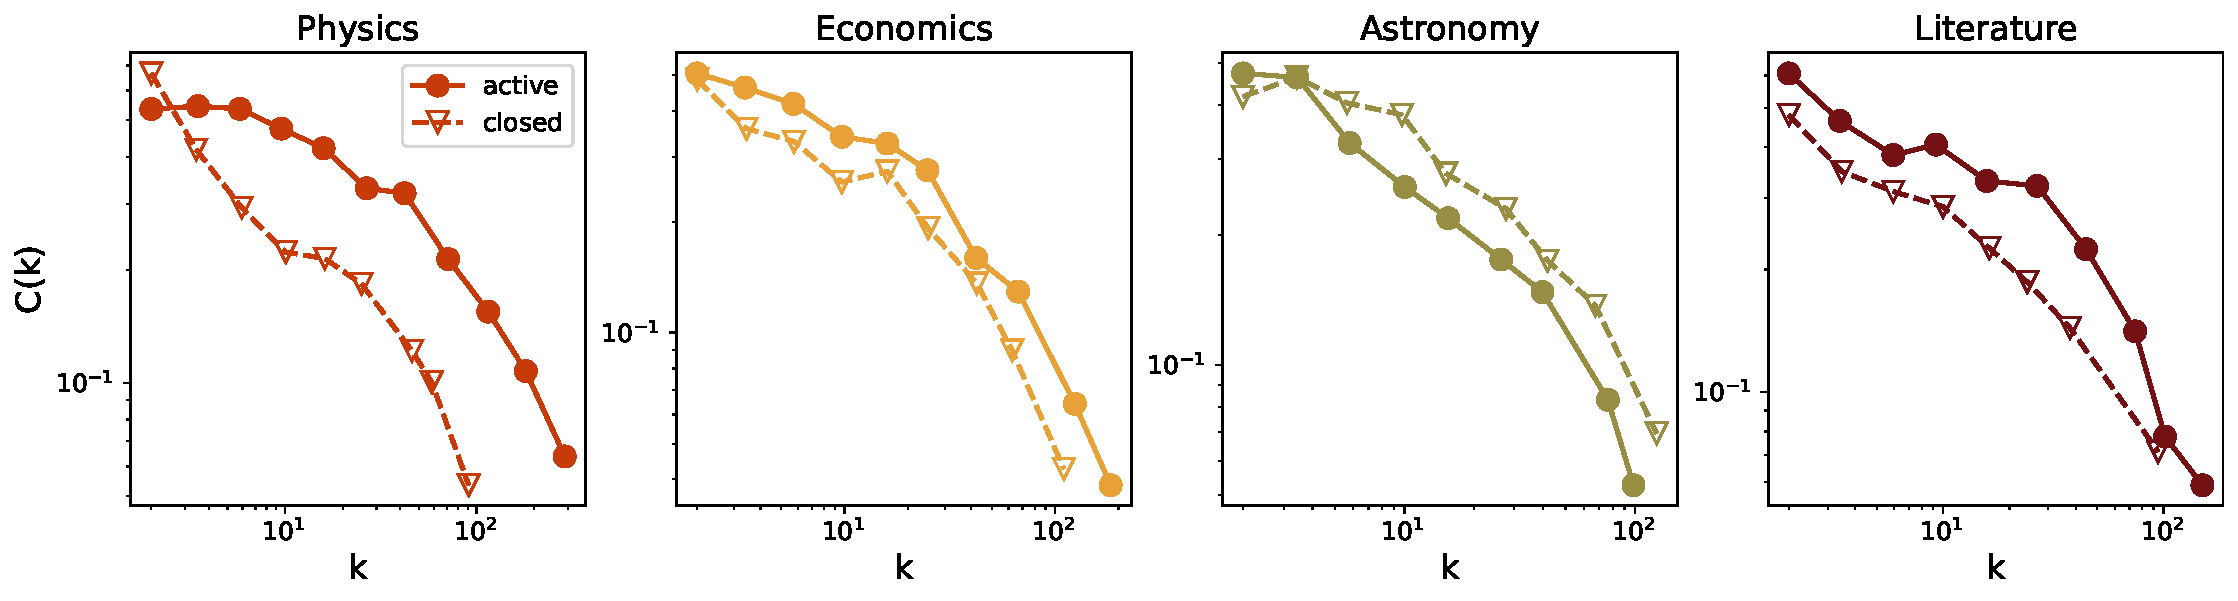
\includegraphics[width=\linewidth]{chapter5/clustering_fullnet.pdf}
	\caption{Clustering coefficient.}
	\label{fig:fullclustering}
\end{figure}

Instead of creating a static network from the data in the first 180 days of community life, we study how network snapshots evolve. At each time step $t$, we create network snapshot $G(t, t+\tau)$ for the time window of the length $\tau$. We fix the time window to $\tau=30$ days and slide it by $t=1$ day through time. A discussion of how the length of the sliding window influences the results is given in Appendix A. Sliding the time window by one day, we can capture changes in the network structure daily, as two 30 days of consecutive networks overlap significantly. 

Here we investigate how the SE community’s clustering coefficient changes with time by calculating its value for all network snapshots. We compare the behaviour of clustering for active and closed communities on the same topic to better understand how the cohesion of these communities is changing over time. Figure \ref{fig:clustering} shows the evolution of the mean clustering coefficient for all eight communities. All communities still alive are clustered, with the value of the mean clustering coefficient higher than 0.1. Physics, the only launched community, has a clustering coefficient value above 0.2 for the first 180 days.

During the larger part of the observed period, an active community’s clustering coefficient is higher than its closed pair’s clustering coefficient. Let’s compare active communities with their closed counterpart. The closed communities have a higher value of the mean clustering coefficient in the early phase, while later communities that are still active have higher clustering coefficient values. These results suggest that all communities have relatively high local cohesiveness and that lower clustering coefficient values may indicate its decline in the later phase of community life. 

\begin{figure}
	\centering
	\includegraphics[width=\linewidth]{chapter5/clustering.pdf}%Figures/figures_SE/Fig3.pdf}
	\caption{Mean clustering coefficient.}
	\label{fig:clustering}
\end{figure}

\section{Core-periphery structure}

Previous research on Stack Exchange communities has attempted to explain how different types of users interact. In Question-Answer communities are expected to be popular and casual users \cite{santos2019activity, santos2019self}. Popular users generate the majority of interactions in the system; they are experts in the community and take care of answering questions and engaging the discussions through comments. As popular users, they considered the $10 \%$ of the most active users and showed that popular users are highly connected with themselves and casual users.

We tested this theory on all eight communities. We focused on 30 days of sub-networks and showed how the Number of links per node among popular users and between popular and casual users evolves, Figure \ref{fig:pop_cas_users}. We also compare active and closed communities of the same topic, so links per node in active sites are more significant than in closed communities.

\begin{figure}[h!]
	\centering
	\includegraphics[width=\linewidth]{chapter5/popular_casual_users.pdf}
	\caption[Number of links per node]{Links per node among popular users (top 10\% of users) and between popular and casual users (everyone but popular users).}
	\label{fig:pop_cas_users}
\end{figure} 

Although we find the difference between active and closed communities, the split according to $10\%$  most active users does not guarantee that all popular users will be considered. Furthermore, the smaller group of frequently active users is similar to the core users in the core-periphery structure. This is why we will detect the core of each 30-day network. By this, separation is based on the network structure and is more consistent, as using the algorithmic approach, we optimize the connectivity inside the core, periphery and among them. The core-periphery structure has a core that is a densely connected group of nodes, while the periphery has a low density \cite{fortunato2010community, gallagher2020clarified}. 

We use the Stochastic Block Model (SBM) to infer the core-periphery structure of each 30 days network snapshot and analyses how the core structure evolves. The  SBM algorithm is adapted for inferring the core-periphery structure, \cite{gallagher2020clarified}. For each 30 days network, we run the sample of 50 iterations and choose the model parameters according to the minimum description length. As stochastic models start from the random configuration, they can converge to different states, so we analyzed the stability of the inferred structures. More details are given in the appendix. We found that obtained structures differ, but the minimum description length does not fluctuate much. Also, different similarity measures between inferred core configurations take values higher than 0.9, indicating that the core structure is stable. 

The Number of users in the core of active communities is higher than in closed communities, the top panel on Figure \ref{fig:core_size}. On the other hand, we do not find a big difference between the fraction of core users in the closed and active communities. Furthermore, the fraction of users in core differs from the $10\%$, and it is constantly changing, bottom panel \ref{fig:core_size}. 

\begin{figure}[h!]
	\centering
	\includegraphics[width=\linewidth]{chapter5/core_users.pdf}
	\caption[The size of the core]{The size of the core (top) and a fraction of users in the core (bottom). Solid lines - active sites; dashed lines - closed sites.}
	\label{fig:core_size}
\end{figure}

The Number of users is constantly changing. To quantify the stability of the core structure, we compute the Jaccard’s coefficient between core users in networks at time points $t_1$ and $t_2$. The Jaccard coefficient range from 0 to 1, so the larger values of the Jaccard index indicate the more similar cores. 
The highest values are found around diagonal elements where we compare networks closer in time, see Figure \ref{fig:jaccard_hm}. The core membership changes over time, and the change is more frequent in closed communities. 

\begin{figure}[h!]
	\centering
	\includegraphics[width=\linewidth]{chapter5/jaccard_heatmap.pdf}
	\caption[Mean Jaccard index between core users.]{Jaccard index between core users in  sub-networks at time points $t1$ and $t2$.}
	\label{fig:jaccard_hm}
\end{figure}  

The average Jaccard index between cores in networks separated by time interval $t_i-t_j$ with the standard deviation confidence interval are shown in Figure \ref{fig:jaccard_mean}. The Jaccard index decreases with the relative time difference between networks faster in closed communities. The relatively high overlap between distant networks confirms that active networks have a more stable core. 

\begin{figure}[h!]
	\centering
	\includegraphics[width=\linewidth]{chapter5/jaccard.pdf}
	\caption[Mean Jaccard index between core users.]{Jaccard index between core users in 30 days sub-networks for all possible pairs of 30 days sub-networks separated by time interval $|t_i - t_j|$.}
	\label{fig:jaccard_mean}
\end{figure}

Finally, we examine how the users’ connectivity in and between the core and periphery evolves. In the Figure \ref{fig:links_per_node}, we show the $L/N$ in the core, which is proportional to the average degree of the network $2L/N$, . The Physics community has more than twice the connectivity than closed Theoretical Physics. For Literature, we also find higher connectivity. Still, at the end of the observation period, the connectivity in the active site drops and becomes similar to that in the closed one. The difference between active and closed sites is unclear for Economics and Astronomy. At the beginning of the period, connectivity is similar for the sites on the economic topic. After 50 days of community life, connectivity in active communities is starting to rise, while in the case of closed economics, it is dropping. Astronomy connectivity is higher in closed communities in the first 50 days. After this period, we find a sudden rise in the connectivity of active astronomy, but again it drops and becomes comparable to the connectivity values in the closed site. Similar conclusions can be drawn for the connectivity between the core and periphery. The largest difference between active and closed sites is observed in Physics.  

\begin{figure}[h]
	\centering
	\includegraphics[width=\linewidth]{chapter5/core_connectivity.pdf}
	\caption{Links per node in core and links per node between core and periphery.}
	\label{fig:links_per_node}
\end{figure}

\section{Dynamical Reputation on Stack Exchange communities}

We further explore the difference between active and closed communities through the dynamic reputation model. With this model, we calculate each user's reputation in the community, and reputation is directly connected with the collective trust in the network. 

\begin{figure}[h]
	\centering
	\includegraphics[width=\linewidth]{chapter5/reputation.pdf}
	\caption[Dynamic Reputation of Stack Exchange websites.]{Dynamic Reputation on the four pairs of Stack Exchange websites: Astronomy, Literature, Economics,  Physics and Theoretical Physics.}
	\label{fig:dr6panel}
\end{figure}

Dynamical reputation model, introduced in section \ref{sec:met_dibrm}, has three parameters. We explored different parameter combinations to find the set of parameters the most suitable for a given system of Stack Exchange communities. First, the basic reputation is set to $I_{bn}=1$. The cumulative factor is $\alpha=2$, as we want to emphasize the frequent interactions. The parameter $\beta$ controls the reputation decay due to user inactivity. After the last activity, the user has a positive reputation for some period and is still impacting the other users. We optimized the Number of users with a reputation larger than $1$ according to the number of users in the 30 days network and concluded that parameter $\beta=0.96$. A more detailed discussion about the choice of parameters is in the appendix \ref{App:parameters}. 

With selected model parameters, we calculated the reputation of each user. If a user has a reputation larger than $1$, it is considered active, but when the reputation drops below this threshold means that the user has not been active long enough; it does not make a valuable contribution to the community. The Number of active users and their mean reputation for different SE sites is shown in Figure \ref{fig:dr6panel}. 

From the properties of networks, we found that active communities are more cohesive and have a more stable core. Furthermore, we focus our analysis on the dynamic reputation of the core users. Figure \ref{fig:dr_core} shows the evolution of mean user reputation within the core. Active communities have a larger reputation than their closed counterpart. As it is previously suggested, the largest difference is found in the Physics community. For other communities, the difference is not so striking; on average, the core of active communities has a larger reputation than the core of closed communities. 

\begin{figure}[h]
	\centering
	\includegraphics[width=\linewidth]{chapter5/core_reputation.pdf}
	\caption{Dynamical reputation within the core.}
	\label{fig:dr_core}
\end{figure}

In the network's core are active users, and we expect a higher dynamic reputation than the total reputation of users belonging to the periphery. The ratio between core and periphery in Physics is always higher than in Theoretical Physics, and similar conclusions are observed in the Literature. In the early days of Economics, we find a different pattern; the core-periphery reputation ratio is larger for closed Economics, but later it changes in favour of active Economics. Astronomy shows different behaviour where the closed community where dominant; closed astronomy had a larger core-periphery reputation ratio. 

\begin{figure}[h!]
	\centering
	\includegraphics[width=\linewidth]{chapter5/core_per_ratio_reputation.pdf}
	\caption[Ratio between the total reputation within network core and periphery.]{Ratio between the total reputation within network core and periphery. Solid lines active communities, dashed lines closed communities.}
	\label{fig:dr_core_per}
\end{figure}

The distribution of the dynamic reputation of SE communities is skewed. We calculated the Gini coefficient to better express the difference between distribution reputations. This measure quantifies the inequality among users’ reputations. The Gini coefficient is calculated based on reputation values for each day; see Figure \ref{fig:dynrep-gini}. The Gini coefficient is larger than $0.5$ in the first 180 days. Also, the active communities showed more reputation inequality, and dynamical reputation has a larger variation. 

\begin{figure}[h]
	\centering
	\includegraphics[width=1\linewidth]{chapter5/gini.pdf}
	\caption[Gini index of dynamic reputation]{Gini index of dynamic reputation within the population.}
	\label{fig:dynrep-gini}
\end{figure} 

Further, we investigate how the properties of user interaction networks correlate with the user’s reputation. For example, we can measure the assortativity coefficient among connected users in the network. For each 30 days user interaction network, we calculate the reputation assortativity, using the reputation value observed on the last day of the time window in which the network is constructed. With this measure, we quantify whether users tend to connect with users with similar reputations or not. Figure \ref{fig:dyn_rep_assort} shows results where we compare each SE community’s active and closed sites. Assortativity has small values in all communities’ reputations, not larger than $|0.3|$. In active communities, this is a mostly negative measure showing expected user behaviour: popular users, who often have a high dynamical reputation, interact with users with low dynamical reputations. Astronomy is an outlier again; during the first 100 days active community had a positive reputation for assortativity, and after this period, it started behaving similarly to other active communities. 

\begin{figure}[h]
	\centering
	\includegraphics[width=1\linewidth]{chapter5/reputation_assortativity.pdf}
	\caption[Dynamic Reputation assortativity]{Dynamic Reputation assortativity in the network of interactions (questions, answers, comments, unweighted, undirected network). Solid lines - active sites; dashed lines - closed sites.}
	\label{fig:dyn_rep_assort}
\end{figure}

Finally, we are interested in how dynamical reputation correlates with network measures. We compare the node’s centrality in the 30-day network and the node’s reputation on the last day of the 30-day sliding window. The correlation coefficient between dynamic reputation and node degree is very high; see the top panel on \ref{fig:dyn_rep_centrality}. The bottom panel shows correlations between dynamic reputation and betweenness centrality in the network, which are also high. We find that correlations are mostly higher in active communities; only for astronomy do they take similar values during the observed period. 

\begin{figure}[h]
	\centering
	\includegraphics[width=\linewidth]{chapter5/correlations.pdf}
	\caption[Coefficient correlation between ]{Coefficient of correlation between users’ Dynamic Reputation and users’ network degree (top) and users’ betweenness centrality (bottom). Solid lines - active sites; dashed lines - closed sites.}
	\label{fig:dyn_rep_centrality}
\end{figure}

\newpage
\section{Conclusions}

The Stack Exchange sites bring together users interested in knowledge sharing. They create different topic communities where each member can post topic-related questions and get the correct answer from other users. The SE developed, in one sense, the trust among users, as many people see the SE as a valuable source of knowledge and seek their answers directly in these communities. Not all SE sites were launched, and some were closed because they did not fulfil the Stack Exchange criteria of the successful community. These criteria rely on basic measures such as the number of active users, posted questions, and answers, so we were interested in investigating the structure and dynamics of SE communities to understand how trustworthy and self-sustainable community emerges. 

This chapter presented results on four pairs of SE communities: Astronomy, Literature, Economics and Physics. The first time each of them failed to create a sustainable network, but later the same topic was proposed communities are still active. While this sample may be small, we wanted to focus only on communities on the same topic, so our comparison between closed and active communities is not topic related. Also, we chose two communities from STEM and two from humanities which allowed us to remove field-related biases. 

We studied how network properties evolve during the first 180 days. To closely examine the structure, we constructed the sub-networks within a 30days window. Sliding window by day, we continuously measure the structure of the network. The clustering coefficient is higher in active communities. The previous study suggested two groups of users in Q-A communities, popular and casual users \cite{santos2019self}. This observation motivated us to closely analyze the network segmentation in the core-periphery structure. Based on Bayesian Stochastic modelling, we identify each 30-day network core user.
Furthermore, using the DIBRM model\cite{melnikov2018toward}, we quantify each user's reputation. This reputation is our proxy of trust, and its dynamics reflect some of the essential properties of trust. When a user is frequently active, the reputation increases; when inactivity declines, the user becomes less important.   

Used methods have several parameters which need to be tuned according to specific systems properties. First of all, we showed that the choice of the sliding window does not influence our conclusions, as observed system properties follow similar patterns for different values of sliding windows. Tuning the DIBRM parameters was more changeling. Our primary assumption was that the number of users with a positive reputation should resemble the number in the 30-day window.

Our results suggest that core members are important for the sustainability of the community. The core members have a high reputation and contribute to the community’s survival. The core is more connected in active communities, and larger connectivity is found between the core and periphery in active communities. The most noticeable difference between closed and active communities is in Physics. Physics is the only community that graduated after 90 days, while other active communities stayed in the beta phase for a couple of years; recently, their status changed to beta. On the other hand, closed Astronomy showed larger network properties than an active one, but as time progressed, this changed in favour of the active community. The larger mean reputation and its dynamics among core users in active networks are important indicators of a thriving community.


%\chapter{Conclusions} % Main chapter title
\label{Ch:Conclussion}

%%TODO: Uvodni pasus
In this thesis, we studied the complex network models to understand the evolution of online social systems. %Considering the properties of the real communities, the evolving network models could be improved and more realistic representations. 
The complex systems change over time, even though we often find the system's collective behaviour that stays universal. The specific interactions among elements could lead to different kinds of organizational patterns. The research from this thesis tries to understand factors that drive the system's growth, change its structural properties and their sustainability.
%contribute to the growth of the systems, structure properties and their sustainability.
%%TODO factors that drive the growth of the system, change of its structure properties and their sustainability.
The underlying methodology is introduced in chapter \ref{Ch:Method}. The first part explained the most important properties of network structure and the growing network models. The second part describes the statistical methods useful for the empirical analysis of the properties of the complex system.  

In chapter \ref{Ch:signals}, we discussed how nonlinear growth signal shapes the structure of the complex network. 
%The previous models combined linking rules with constant growth, but we added one more parameter, the fluctuating growth signals, in this research. 
%%TODO Ovu recenicu bih malo drugacije: 
The previous models combined linking rules with constant growth; however, empirical analysis of various real systems and agent-based simulation \cite{mitrovic2012, mitrovic2015} have indicated that properties of growth signal influence the dynamics of complex systems, as well as the structure of its interaction network. To investigate the connection between the features of the growth signal and the structure of an evolving network, we added one more parameter in the growth of the aging network model, the fluctuating growth signal, and examined how network properties change with the signal.
The most considerable influence is found on scale-free networks. Many interaction networks from social, technological or biological systems have scale-free structure; they are correlated and clustered. These results suggested that it is important to study growing signals' properties. Signals from natural systems show trends and cycles and are characterized by long-range correlations. The structure of the generated complex networks depends on the signal properties, and it is necessary to quantify these properties as they affect the network's topology differently. For example, the most significant difference between networks generated with fluctuating and constant signals is found for signals with multi-fractal properties. This difference is more negligible for monofractal signals or uncorrelated white noise. Fluctuating signals promote the creation of hubs in the network and shorten the paths between nodes.

Chapter \ref{Ch:Groups} presented the results of the universal characteristics of the growth of online social groups—the growth of the system influence the structure of the interaction network. The distribution of the sizes of the complex systems usually follows some universal curve. In many cases, it is lognormal or power-law. The distribution of the dimensions of the city sizes could be explained with Zipf law \cite{gabaix1999}. The number of citations scales as lognormal distribution \cite{radicchi2008}. In this thesis, we empirically analyzed the growth of online social systems. They consist of groups whose growth is universal. The empirical analyses of Meetup groups and Reddits showed their group size distribution follows universal lognormal distribution, stable over time. This research aimed to examine the structure and dynamics of the interaction network. We proposed the bipartite group model to gain a deeper understanding of the factors that affect the growth of social groups in a complex system. The growth in this model is driven by fluctuating signals, similar to the paper presented in chapter 2: we use a time series of new members from Meetup and Reddit. The number of groups also grows as each user can create a new one; otherwise, the user joins the old group, and different linking rules determine his decision. The lognormal distribution of the group sizes emerges when with probability $p_{aff}$, users prefer groups whose friends are already members, while with probability $1-p_{aff}$, their choice is random. The width of the lognormal distribution depends on the parameter $p_{aff}$. The systems influenced more by social connections have larger $p_{aff}$, and the broader group sizes have lognormal distribution.

In chapter \ref{Ch:Trust}, we focused on the factors that influence the sustainability of evolving complex networks. Specifically, we investigated the sustainability of social groups on the Question-Answers platform Stack Exchange. 
%on the Question-Answers platform Stack Exchange.
%%TODO we focused on the factors influencing the sustainability of evolving complex networks. Specifically, we investigated the sustainability of social groups on the Question-Answers platform Stack Exchange.
Each site goes through several phases before being successful and launched. During that period, the site may be closed. We selected several topics in which sites for the first time were closed, but in the second attempt, they survived and are still active. We provide a detailed analysis of active and closed Stack Exchange sites, compare their properties and identify what is crucial for the community's survival. We map user interactions observed in 30 days onto complex networks. Further, we slide the window by one day and follow the evolution of the network. 

According to the clustering properties of these networks, sustainable communities have a higher value of local cohesiveness. We use the Bayesian stochastic block modelling approach~\cite{gallagher2020clarified} to determine the core-periphery structure of these networks. We find that sustainable communities develop stable, better-connected cores. To analyze the evolution of collective trust in SE communities, we modify the Dynamic InteractionBased Reputation Model~\cite{melnikov2018toward} (DIBR) model. We use the DIBR model to measure the user's reputation based on the frequency of their activity and its evolution during the first 180 days. The trust between core members of active communities develops early and is higher than in closed communities during the first 180 days. The early emergence of a stable, trustworthy core may be a crucial factor in determining a knowledge-sharing community's sustainability. 

%%TODO: Pasus koji opisuje next directions 
The question raised by this study is how trust emerges among users in questions answers communities where the users tend to share knowledge, and their communication is neutral or positive. Some communities started promoting hate speech on different online platforms, resulting in the banning. But, banned users remained in the online world; they moved their communities to alternative platforms without strict policies, such as Voat. Later, Voat users also formed no-hate speech topics, and there is an open question does the emergence of trust differ among different communities? On the other hand, exploring higher-order representations of online communities would be interesting. Threads, where more people reply to one post, could be studied using simplicial complexes to reveal complex network structure patterns. Furthermore, the research that employs agent-based modelling allows us to connect closer the actions of single users with the emergence of collective phenomena and the rise and fall of trust in the system. 

The results from this thesis contribute to the knowledge about complex network structure and dynamics. We explored different factors that influence network growth, structural properties and sustainability. The growth signal impacts the network's structural properties, while social interactions affect group segmentation. The sustainability of evolving networks depends on core-periphery structure, the core's stability and users' ability to form a trustworthy core. Research presented in this thesis confirms that dynamics is linked with the structure of its interaction network, while the structure directly determines the function, organization and sustainability of complex systems.  

%TODO Ovo je OK ako bi teza bila poverenjju. Mozes ostaviti ovaj paragraf, ali nesdotaju jos dve. 

%TODO Prvi paragraf koji sumira sve tri stvari, nesto u skladu sa ovih par recenica:%
%TODO %"In this thessis, we have explored different factors that influence the growth, structure and sustainability of complex networks. Our results show that growth signal critical influence on the structure of evolving networks, while their segmentation into social groups is influenced by social factors. The sustainability of evolving complex networks is influenced both by its core-periphery structure and stability of the core, as well as the ability of users to form cohesive trustworthy core. Research presented in this thesis confirms once more that dynamics of a complex system is inextricably linked with the structure its interaction network, Furthermore, our results show that the the structure of a complex network determines the function, organization and sustainability of a complex system."

%TODO I treba nam dodatni paragraf sa otvorenim pitanjima. Ovo moram da razmislim malo, ali ako ti nesto padne na pamet, slobodno napisi.

Complex network theory is a rapidly growing field, but many open research questions exist. With the increase in the availability of the data of various complex systems, the analysis of complex networks becomes even more popular and shows excellent potential for future work. While we mostly understand how to describe the network's structure, and many methods are adapted to deal with evolving complex networks, we still need insights into how to design networks to control their properties to prevent outbreaks or enhance information diffusion. Developing models incorporating spatial or temporal constraints could provide a more accurate picture of systems evolution. Community detection methods are beneficial for understanding network structure and function, it lacks methods that easily adapt to network changes over time. The current development of machine learning on graphs could fill existing gaps and provide more accurate predictions of complex network systems behavior.

\selectlanguage{serbianc}
\sffamily
\fontencoding{OT2}\fontfamily{Tempora-TLF}\selectfont

\selectlanguage{english}

	
%end{itemize}



\appendix
%\chapter{Stack Exchange}
\label{App:SE}
Stack Exchange data are public and regularly released. As closed communities were active between 180 and 210 days, we extracted only the first 180 days of data. Given that the first few months can be crucial for the further development of the community \cite{dover2020sustainable}, we are interested in the early evolution of Stack Exchange sites. 

Detailed information about questions, answers, and comments is available for each SE community. Each post is labelled with a unique ID, the user's ID who made the post, and the creation time. On Stack Exchange, users interact on several layers and those interactions are considered positive:
\begin{itemize}
	\item Posting an answer to the question; for every question, we extract the IDs of its answers
	\item Posting a comment on the question or answer; for every question and answer, we selected the IDs of its comments
	\item Accepting answer; for each question, we selected the accepted answer ID
\end{itemize}

Even though posts can be voted on and downvoted, information about a user who voted is absent, so we do not consider these interactions between users. Comments can not be downvoted, while we find only around 3\% negatively voted answers and questions, Table \ref{tab:negint}.

\begin{table}[hbt!]
	\centering
	\caption{Percentage of negatively voted interactions.}
	\label{tab:negint}
	\begin{tabular}{cc|cc}
		
		\hline
		Site                        & Status & Questions & Answers \\ \hline
		\multirow{2}{*}{Physics}    & Beta   & 5\%       & 4\%     \\
		& Closed & 1\%       & 2\%     \\ \hline
		\multirow{2}{*}{Astronomy}  & Beta   & 3\%       & 3\%     \\
		& Closed & 2\%       & 1\%     \\ \hline
		\multirow{2}{*}{Economics}  & Beta   & 4\%       & 4\%     \\
		& Closed & 7\%       & 4\%     \\ \hline
		\multirow{2}{*}{Literature} & Beta   & 2\%       & 5\%     \\ 
		& Closed & 2\%       & 1\%     \\ \hline \hline
		\textbf{Average}            &        & 3.2\%     & 3\%     \\ \hline 
	\end{tabular}
\end{table}


%The data contains information about the official StackExchange reputation of each user but only as a single value measuring the final reputation of the user on the day when the data archive was released. Because of this significant shortcoming, we do not include this information in our analysis. In SE, users can give positive or negative votes to questions and answers and mark questions as a favour; however, the data is again provided as a final score recorded at the moment of the realise of the database. Since this does not allows us to analyze the evolution of scores, we omit this data from our analysis.\\


\section{Comparison between active and closed SE communities}

Table \ref{tab:site-info} compares the first 180 days between closed and active communities. Regarding basic statistics, active communities had a larger number of users, questions, answers and comments. Another simple indicator if the community will graduate or decline can be time series of active questions for seven days in Figure \ref{fig:active_questions}. The question is active if it had at least one activity, posted answer, or comment during the previous seven days. We find that live communities have more active questions after the first three months. Still, this difference is smaller for literature and astronomy. For astronomy, we observe that closed communities had more active questions in the early period of community life.


\begin{table}[h]
	\centering
	\caption[Community overview for first 180 days.]{Community overview for first 180 days, Number of users $n_u$, number of questions $n_q$, number of answers $n_a$, number of comments $n_c$.}
	\label{tab:site-info}
	\begin{tabular}{llccccc}
		\toprule
		Site                 & Status                           & First Date                     & $n_u$                    & $n_q$                & $n_a$                  & $n_c$ \\ \hline
		\multirow{2}{*}{Astronomy}  & \multicolumn{1}{l|}{Closed}      & \multicolumn{1}{c|}{09/22/10} & \multicolumn{1}{c|}{336}  & \multicolumn{1}{c|}{474}  & \multicolumn{1}{c|}{953}  & 1444     \\
		& \multicolumn{1}{l|}{Beta} & \multicolumn{1}{c|}{09/24/13} & \multicolumn{1}{c|}{405}  & \multicolumn{1}{c|}{644}  & \multicolumn{1}{c|}{959}  & 2170     \\ \hline
		\multirow{2}{*}{Economics}  & \multicolumn{1}{l|}{Closed}      & \multicolumn{1}{c|}{10/11/10} & \multicolumn{1}{c|}{275}  & \multicolumn{1}{c|}{368}  & \multicolumn{1}{c|}{458}  & 1253     \\
		& \multicolumn{1}{l|}{Beta} & \multicolumn{1}{c|}{11/18/14} & \multicolumn{1}{c|}{648}  & \multicolumn{1}{c|}{1024} & \multicolumn{1}{c|}{1410} & 3553     \\ \hline
		\multirow{2}{*}{Literature} & \multicolumn{1}{l|}{Closed}      & \multicolumn{1}{c|}{02/10/10} & \multicolumn{1}{c|}{284}  & \multicolumn{1}{c|}{318}  & \multicolumn{1}{c|}{523}  & 1097     \\
		& \multicolumn{1}{l|}{Beta} & \multicolumn{1}{c|}{01/18/17} & \multicolumn{1}{c|}{478}  & \multicolumn{1}{c|}{910}  & \multicolumn{1}{c|}{907}  & 3301     \\ \hline
		\multirow{2}{*}{Physics}    & \multicolumn{1}{l|}{Closed}      & \multicolumn{1}{c|}{09/14/11} & \multicolumn{1}{c|}{281}  & \multicolumn{1}{c|}{349}  & \multicolumn{1}{c|}{564}  & 2213     \\
		& \multicolumn{1}{l|}{Launched}    & \multicolumn{1}{c|}{08/24/10} & \multicolumn{1}{c|}{1176} & \multicolumn{1}{c|}{2124} & \multicolumn{1}{c|}{4802} & 15403    \\
		\bottomrule
	\end{tabular}
\end{table}


\begin{figure}
	\centering
	\includegraphics[width=\linewidth]{appendixA/active_questions.pdf}
	\caption[Number of active questions within seven days sliding windows.]{Number of active questions within seven days sliding windows. Solid lines - active sites; dashed lines - closed sites.}
	\label{fig:active_questions}
\end{figure}

Similarly, the official Stack Exchange community evaluation process considers simple metrics \footnote{\href{https://stackoverflow.blog/2011/07/27/does-this-site-have-a-chance-of-succeeding/}{https://stackoverflow.blog/2011/07/27/does-this-site-have-a-chance-of-succeeding/}}. To determine the success of sites they measure how many questions are answered, how many questions are posted per day, and how many answers are posted per question. There are two measures: the number of avid users and the number of visits that are not easily interpreted from the data. The site is \textit{healthy} if it has ten questions per day, 2.5 answers per question and more than $90\%$ of answered questions. For less than $80\%$ of answered questions, five questions per day and 1 question per answer site \textit{needs some work}. 

We calculated Stack Exchange statistics for astronomy, economics, literature and physics and results are presented in Table \ref{tab:se_c}. After 180 days, only live physics is a healthy site while other live communities are at least in two criteria labelled as \textit{okay}. Closed sites mostly \textit{need some work}; the exception is closed astronomy. For example, it has \textit{excellent} percent of answered questions and \textit{okay} answer ratio.  

%While the Physics community was more successful than Theoretical Physics and other considered communities, these differences are not as clear if we compare three different pairs of communities. For instance, some of the parameters for a closed Astronomy community were better than for the still active community. Similar results were found for Economics and Literature. 

\begin{table}[h!]
	%\footnotesize\sf\centering
	\caption{Community overview for first 180 days according to SE criteria.}
	
	\label{tab:se_c}
	\begin{tabular}{ccccc}
		\hline
		
		Site & Status &  Answered & Questions per day & Answer ratio \\ \hline
		\multirow{2}{*}{Astronomy} & \multicolumn{1}{c|}{Closed} & \multicolumn{1}{c|}{\textbf{95} \%}  & \multicolumn{1}{c|}{2.62} & \multicolumn{1}{c}{\underline{2.02}} \\
		& \multicolumn{1}{c|}{Beta} & \multicolumn{1}{c|}{\textbf{96} \%}  & \multicolumn{1}{c|}{3.57} & \multicolumn{1}{c}{\underline{1.49}} \\ \hline
		\multirow{2}{*}{Economics} & \multicolumn{1}{c|}{Closed} & \multicolumn{1}{c|}{68 \%}  & \multicolumn{1}{c|}{2.04} & \multicolumn{1}{c}{\underline{1.25}} \\
		& \multicolumn{1}{c|}{Beta} & \multicolumn{1}{c|}{\underline{84} \%}  & \multicolumn{1}{c|}{\underline{5.66}} & \multicolumn{1}{c}{\underline{1.37}} \\ \hline
		\multirow{2}{*}{Literature} & \multicolumn{1}{c|}{Closed} & \multicolumn{1}{c|}{79 \%}  & \multicolumn{1}{c|}{1.77} & \multicolumn{1}{c}{\underline{1.65}} \\
		& \multicolumn{1}{c|}{Beta} & \multicolumn{1}{c|}{74 \%}  & \multicolumn{1}{c|}{\underline{5.04}} & \multicolumn{1}{c}{\underline{1.10}} \\ \hline
		\multirow{2}{*}{Physics} & \multicolumn{1}{c|}{Closed} & \multicolumn{1}{c|}{83 \%}  & \multicolumn{1}{c|}{1.93} & \multicolumn{1}{c}{\underline{1.64}} \\
		& \multicolumn{1}{c|}{Beta} & \multicolumn{1}{c|}{\textbf{93} \%}  & \multicolumn{1}{c|}{\textbf{11.76}} & \multicolumn{1}{c}{ \textbf{2.74}} \\ \hline \hline
		{Stack Exchange criteria} & excellent & $>$ 90 \% & $>$10 & $>$ 2.5   \\
		& needs some work & $<$ 80 \% & $<5$ & $<$ 1   \\ \hline
		
		
	\end{tabular}
	
\end{table}

These simple measurements presented in tables \ref{tab:site-info} and \ref{tab:se_c} and Figure \ref{fig:active_questions} do not provide us clear indications about community sustainability. Only for physics topics the difference between active and closed communities is evident, while for other communities, it is not so clear. Thus, we need deeper insights into the structure and dynamics of these communities to understand. The structure of social interactions within communities and the dynamics of collective trust may provide a better explanation of why some communities succeed, and others die. 
%\chapter{The choice of the sliding window} % Main chapter title
\label{App:sliding}

To study the evolution of Stack Exchange communities, we chose to at each time step $t$ analyze the structure of interaction networks created in the period $[t, t+\tau)$. By this, we have better insight into how network properties evolve. However, it is not defined what value the sliding window should take. The previous studies showed that the value of a sliding window determines how much information is saved. If $\tau$ is small, sub-networks are sparse, while for a large sliding window, important changes in the measures may not be detected \cite{krings2012effects, arnold2021moving}. We analyze how network properties and dynamic reputation depend on the window size. For example, we use Astronomy and compare the active and closed communities, Figure \ref{fig:windows} Similar conclusions can be observed for other pairs of communities. The time window of 30 days approximates one month.  

We show the network properties for sub-networks of 10, 30, and 60 days sliding windows. For a sliding window of 10 days, results may be too noisy, and we may not observe some important trends in the community. The number of users for beta astronomy seems to fluctuate around some mean value. On the larger scale, 30 days window,  it is more apparent that the number of users slightly increases over time. Contrary, for too large an aggregation window (60 days), important information about the time series can be lost, such as the local minimum of the number of users around time step 80 that is observed for the 30-day sliding window. 
From network measures such as L/N and clustering, we conclude that the difference between closed and active sites is more transparent with a larger aggregation window. Still, on each scale, beta sites show a higher number of nodes, number of links per node and clustering coefficient.

As before, we study the structure of created sub-networks through the lens of core-periphery structure. On small scales, within the window of 10 days, there are often few or even no nodes in the core, and it can affect the calculation of other measures of interest. Such behaviour is more typical for closed communities. With the size of the sliding window, the number of nodes in the core increases and the results of core-periphery measures and dynamical reputation between core users and between core and periphery users become smoother. Finally, the choice of the sliding window does not change the conclusion that core users in the beta communities produce more activity and make a strong core. However, our main results are shown for a sliding window of 30 days, as it creates a good compromise between large and small time scales.   

\begin{figure}[!ht]
	\centering
	\includegraphics[width=0.9\linewidth]{figures/stackexchange/sliding_window.pdf}
	\caption[Stack Exchange properties for different sliding window.]{Results for different sliding windows. For astronomy, solid blue lines- active, orange dashed lines - closed site. }
	\label{fig:windows}
\end{figure}

%\chapter{Robustness of core-periphery algorithm} % Main chapter title
\textbf{Precision and recall}

Consider the network $G(V, L)$, with a set of nodes $V$ and a set of links between them $L$. The stochastic community detection algorithms may converge to different configurations. To quantify the similarity between the obtained structures and robustness of the algorithm, we run 50 iterations and calculate several similarity measures between pairwise partitions $C$ and $C^{'}$.

The core-periphery structure has two groups so confusion matrix \cite{labatut2012accuracy} can be defined as:

\begin{center}
	
	\begin{tabular}{l|l|c|c|c} 
		
		\multicolumn{2}{c}{}&\multicolumn{2}{c}{partition C}&\\ 
		
		\cline{3-4} 
		\multicolumn{2}{c|}{}&core&periphery&\multicolumn{1}{c}{}\\
		\cline{2-4} 
		partition & core & $n_{TP}$ & $n_{FN}$ & \\ 
		\cline{2-4} $C^{'}$ & periphery & $n_{FP}$ & $n_{TN}$ & \\ 
		\cline{2-4}
	\end{tabular}
\end{center}

The diagonal elements correspond to the number of nodes found in the same class in both node configurations. The number of nodes in the core found in $C$ and $C^{'}$ is denoted as true positive $n_{TP}$, while the number of nodes in the periphery in $C$ and $C^{'}$ is denoted as true negative $n_{TN}$. The off-diagonal elements of the confusion matrix indicate the number of nodes differently classified. We can define the number of nodes found in the first configuration C in the core but in $C^{'}$ in the periphery as a false positive, $n_{FP}$, similarly the number of nodes found in the periphery in the partition $C$, and in the core in partition $C^{'}$ as a false positive, $n_{FP}$. 

From the confusion matrix, we can write the precision $P =n_{TP}/(n_{TP}+n_{FP})$ and recall $R=n_{TN}/(n_{TN}+n_{FN})$. These measures range from 0 to 1. The precision (recall) corresponds to the proportion of instances predicted to belong (not belong) to the considered class and which indeed do (do not) \cite{labatut2012accuracy}. \\~\\

The \textbf{F1 measure} is the harmonic mean of precision and recall \cite{labatut2012accuracy}:
\begin{equation}
F_1 = 2\frac{P \cdot R}{P+R} = \frac{2n_{TP}}{2n_{TP}+n_{FN} + n_{FP}}
\end{equation}
It can be interpreted as a measure of overlap between true and estimated classes; it is 0 for no overlap to 1 if overlap is complete.\\~\\

The \textbf{Jaccard's} coefficient is the ratio of two classes' intersection to their union \cite{labatut2012accuracy}. It can also be expressed in terms of confusion matrix: 
\begin{equation}
J =  \frac{C_{core} \cap C^{'}_{core}}{C_{core} \cup C^{'}_{core}} =   \frac{n_{TP}}{n_{TP}+n_{FP} + n_{FN}}
\end{equation}
\\~\\
\textbf{Normalized mutual information (NMI)} is similarity measure between to partitions $C$ and $C^{'}$  based on information theory \cite{danon2005comparing}:

\begin{equation}
NMI(C, C^{'}) = \frac{MI(C, C^{'})}{(H(C)+H(C^{'})/2}
\end{equation}

where $MI$ is mutual information between sets $C$ and $C^{'}$, while $H(C)$ is entropy of given partition. The entropy is defined as $H(C) = - \sum_{i=1}^{|C|}P(i)log(P(i))$, where $P(i) = |U_i|/N$ is the probability that an object is randomly classified as $i$ (in this special case $i=0$, the node belongs to the core, or $i=1$, the node belongs to the periphery). The mutual information between sets $C$ and $C^{'}$ measures the probability that the randomly chosen node is a member of the same group in both partitions:
\begin{equation}
MI(C, C) = \sum_i\sum_j P(i, j) log(\frac{P(i,j)}{P(i)P^{'}(j)})    
\end{equation}
where $P(i, j)= |U_i \cap U_j|/N$

$NMI$ ranges from 0 when the partitions are independent to 1 if they are identical.   
\\~\\
\textbf{Adjusted rand index.} For the set of nodes $V$, with $n$ nodes, consider all possible combination of pairs $(v_i, v_j)$. We can select the number of the pairs where nodes belong to the same group in both partitions, $C$ and  $C^{'}$, denoted as $a$. Similarly, as $b$, we can define the number of pairs whose nodes belong to different groups in partitions. Then, unadjusted rand index \cite{santos2009use} is given as $RI = \frac{a+b}{\binom{n}{2}}$, where $\binom{n}{2}$ is number of all possible pairs. The RI between two randomly assigned partitions is not close to zero; for that reason, it is common to use the adjusted rand index \cite{hubert1985comparing} , defined as:
\begin{equation}
ARI = \frac{RI - E[RI]}{max(RI)- E[RI]}
\end{equation}
where $E[RI]$ is expected value of RI, and $max(RI)$ is maximum value of $RI$. 

\clearpage
As example we show analysis of inferred sample of  core-periphery structures for 30 days closed Astronomy, Stack Exchange networks, Figure \ref{fig:sample}. We represent the mean minimum description length (MDL) and the mean number of nodes in the core with standard deviation. MDL does not change much between inferred core-periphery structures; the difference between obtained configurations is still notable in the number of nodes in the core.  To investigate in more details similarity between obtained core-periphery configurations in the sample we calculate several measures between pair-wise partitions such as normalized mutual information, adjusted rand index, F1 measure and Jaccard index. These measures are greater than 0.5 and, in most cases, greater than 0.9, indicating stability of the inferred core-periphery structures.


\begin{figure}[h]
	\centering
	\includegraphics[width=0.8\linewidth]{figures/stackexchange/blockmodel_robust.pdf}
	\caption{Minimum description length, number of nodes in core, normalized mutual information, adjusted rand index, F1 measure and Jaccard index, among 50 samples for 30-days sub-networks. Results are given for closed astronomy. }
	\label{fig:sample}
\end{figure}


\backmatter

%References
\bibliographystyle{unsrt}
\bibliography{sample}

%\selectlanguage{english}

\normalsize

\chapter{Biography of the author}

Ana Vranić was born on November 23rd, 1993, in Čacak, Republic of Serbia, where she finished elementary and high school. In 2012 she enrolled BSc studies of Theoretical and Experimental Physics at the Faculty of Physics Belgrade and graduated in 2016 with a GPA of 9.24/10.00. In the same year, she started MSc studies at the Faculty of Physics and, after one year, finished them with a GPA of 10.00/10.00. Her master thesis, "Thermodynamics and electronic transport in Habard model on the triangular lattice", was done under Dr. Darko Tanasković in Scientific Computing Laboratory at the Institute of Physics Belgrade. During this research, she visited the institute Jožef Stefan in Ljubljana, for which she received the CEEPUS scholarship. Ana also won the "Prof. dr Ljubomir Ćirković" foundation award for best MSc thesis defended at the Faculty of Physics of the University of Belgrade.

In 2017, Ana Vranić started PhD studies at the Faculty of Physics in statistical physics. Under the supervision of Dr. Marija Mitrović Dankulov at the Institute of Physics Belgrade. Since April 2018 Ana has been employed at the Institute of Physics Belgrade as a Research Assistant in the Scientific Computing Laboratory of the National Center of Excellence for the Study of Complex Systems. She participated in several projects:  the National Project ON171017 Modeling and Numerical Simulations of Complex Many-Body Systems, funded by the Ministry of Education, Science and Technological Development of the Republic of Serbia; Artificial Intelligence Theoretical Foundations for Advanced Spatio-Temporal Modelling of Data and Processes (ATLAS) project funded by the Science Fund of the Republic of Serbia and in REmote development of Autonomous Driving algorithms in a realistic environment (READ) project funded by Innovation Fund of Republic Serbia.

Ana Vranić has published four papers in peer-reviewed international journals. Papers (1-3) are part of this thesis, while the 4th paper presents research done during MSc studies. She also presented her research at several international conferences.

\begin{enumerate}
	\item \textbf{Vranić A}, Tomašević A, Alorić A, Mitrović Dankulov M. Sustainability of Stack Exchange Q$\&$A communities: the role of trust. EPJ Data Science. 2023 Feb 24;12(1):4.
	
	
	\item \textbf{Vranić A}, Smiljanić J, Mitrović Dankulov M. Universal growth of social groups: empirical analysis and modeling. Journal of Statistical Mechanics: Theory and Experiment. 2022 Dec 7;2022(12):123402.
	
	\item \textbf{Vranić A}, Mitrović Dankulov M. Growth signals determine the topology of evolving networks. Journal of Statistical Mechanics: Theory and Experiment. 2021 Jan 22;2021(1):013405.

	\item \textbf{Vranić A}, Vučičević J, Kokalj J, Skolimowski J, Žitko R, Mravlje J, Tanasković D. Charge transport in the Hubbard model at high temperatures: Triangular versus square lattice. Physical Review B. 2020 Sep 21;102(11):115142.
\end{enumerate}

%\let\cleardoublepage\clearpage


\newpage
~
\selectlanguage{english}
\thispagestyle{empty}

%\selectlanguage{serbianc}

\cleardoublepage

\thispagestyle{empty}
\setlength{\parindent}{0pt}

\renewcommand{\headrulewidth}{0pt}


\normalsize

\mbox{}\pdfbookmark[0]{Izjava o autorstvu}{autorstvo}
\vspace{1cm}


\begin{center}
\begin{Large}\textbf{Изјава о ауторству}
\end{Large}\end{center}

\vspace{1.5cm}

Име и презиме аутора -- \textbf{Ана Вранић}

Број индекса -- \textbf{2017/8006}

\vspace{.7cm}

\begin{center}
\textbf{Изјављујем}            \end{center}

да је докторска дисертација под насловом 


\textbf{\selectlanguage{english} Evolving complex networks: structure and dynamics}


\textbf{(Растуће комплексне мреже: структура и динамика)}

\begin{itemize}
 \item резултат сопственог истраживачког рада;
\item  да дисертација у целини 
ни у деловима није била предложена за стицање друге дипломе према студијским 
програмима других високошколских установа;
\item да су резултати коректно наведени и 
\item да нисам кршила ауторска права и користила интелектуалну својину 
других лица.
\end{itemize}

\vfill
 
У Београду, \hspace{1cm} 2023.  \hfill  \textbf{Потпис
аутора\hspace{2cm}\mbox{}}

\vspace{.5cm}
\hspace{10cm}\hrulefill 

\hspace{\fill}
%\pagebreak
%\justify

%\let\cleardoublepage\clearpage


%\selectlanguage{serbianc}
\cleardoublepage

\thispagestyle{empty}
\setlength{\parindent}{0pt}
\renewcommand{\headrulewidth}{0pt}


\normalsize

\mbox{}\pdfbookmark[0]{Izjava o istovetnosti}{istovetnost}
\vspace{1cm}

\begin{center}


\begin{Large}\textbf{Изјава o истоветности штампане и електронске верзије 
докторског рада 
}
\end{Large} 
\end{center}


\vspace{1cm}

Име и презиме аутора -- \textbf{Име Презиме}

Број индекса -- \textbf{ХХХХХХХХХХХХ}

Студијски програм --  Физика кондензоване материје и статистичка физика

Наслов рада -- 
{\selectlanguage{english}
\textbf{English title of thesis}}

\textbf{(Српски наслов рада)}

Ментор -- \textbf{др Петар Петровић}

Изјављујем  да  је  штампана  верзија  мог  докторског  рада  истоветна  
електронској верзији  коју  сам  предала  ради  похрањивања у \textbf{Дигиталном 
репозиторијуму Универзитета у Београду}. 

Дозвољавам да се објаве моји лични 
подаци везани за добијање академског назива доктора наука, као што су име и 
презиме, година и место рођења и датум одбране рада. 

Ови лични подаци могу се 
објавити на мрежним страницама дигиталне библиотеке, у електронском каталогу и 
у 
публикацијама Универзитета у Београду.
 

\vfill

У Београду, \hspace{1cm} 2023  \hfill  \textbf{Потпис
аутора\hspace{2cm}\mbox{}}

\vspace{.5cm}
\hspace{10cm}\hrulefill 


\hspace{\fill}
%\pagebreak
%\justify
\let\cleardoublepage\clearpage



%\selectlanguage{serbianc}

\cleardoublepage
\thispagestyle{empty}

\renewcommand{\headrulewidth}{0pt}
\setlength{\parindent}{0pt}

\normalsize

\mbox{}\pdfbookmark[0]{Izjava o korišćenju}{koriscenje}
\vspace{1cm}

\begin{center}
\begin{Large}\textbf{Изјава о коришћењу}
\end{Large}\end{center}

\vspace{1cm}

Овлашћујем Универзитетску библиотеку „Светозар Марковић“ да у Дигитални 
репозиторијум Универзитета у Београду унесе моју докторску дисертацију под 
насловом:

{\selectlanguage{english}
\textbf{Evolving complex networks: structure and dynamics}}

\textbf{(Растуће комплексне мреже: структура и динамика)}

која је моје ауторско дело. 

Дисертацију са свим прилозима предала сам у електронском формату погодном за 
трајно архивирање. 

Моју докторску дисертацију похрањену у Дигиталном репозиторијуму Универзитета у 
Београду и доступну у отвореном приступу могу да користе сви који поштују 
одредбе садржане у одабраном типу лиценце Креативне заједнице {\selectlanguage{english}(Creative Commons)} 
за коју сам се одлучила.
\begin{enumerate}[leftmargin=0.5cm]
 \item Ауторство {\selectlanguage{english}(CC BY)}
 \item Ауторство -- некомерцијално {\selectlanguage{english}(CC BY-NC)}
 \item Ауторство -- некомерцијално -- без прерада {\selectlanguage{english}(CC BY-NC-ND)}
 %\renewcommand{\labelenumi}{\circled{\oldlabelenumi}}
 \textbf{\item  Ауторство -- некомерцијално -- делити под истим условима  {\selectlanguage{english}(CC BY-NC-SA)}}
%\renewcommand{\labelenumi}{\oldlabelenumi}
\item  Ауторство --  без прерада {\selectlanguage{english}(CC BY-ND)}
\item  Ауторство --  делити под истим условима {\selectlanguage{english}(CC BY-SA)}
 \end{enumerate}
(Молимо да заокружите само једну од шест понуђених лиценци. \\
Кратак опис лиценци је саставни део ове изјаве).



\vfill

 
У Београду, 13.03.2023.  \hfill  \textbf{Потпис
аутора\hspace{2cm}\mbox{}}

\vspace{.5cm}
\hspace{10cm}\hrulefill 

\hspace{\fill}

\pagebreak
\thispagestyle{empty}


\begin{enumerate}[leftmargin=0.5cm]
\item \textbf{Ауторство.} Дозвољавате умножавање, дистрибуцију и јавно 
саопштавање дела, и 
прераде, ако се наведе име аутора на начин одређен од стране аутора или даваоца 
лиценце, чак и у комерцијалне сврхе. Ово је најслободнија од свих лиценци.
\item \textbf{Ауторство -- некомерцијално.} Дозвољавате умножавање, 
дистрибуцију и јавно 
саопштавање дела, и прераде, ако се наведе име аутора на начин одређен од 
стране 
аутора или даваоца лиценце. Ова лиценца не дозвољава комерцијалну употребу дела.
\item \textbf{Ауторство -- некомерцијално -- без прерада.} Дозвољавате 
умножавање, 
дистрибуцију и јавно саопштавање дела, без промена, преобликовања или употребе 
дела у свом делу, ако се наведе име аутора на начин одређен од стране аутора 
или 
даваоца лиценце. Ова лиценца не дозвољава комерцијалну употребу дела. У односу 
на све остале лиценце, овом лиценцом се ограничава највећи обим права коришћења 
дела. 
\item \textbf{Ауторство -- некомерцијално -- делити под истим условима.} 
Дозвољавате умножавање, дистрибуцију и јавно саопштавање дела, и прераде, ако се 
наведе име 
аутора на начин одређен од стране аутора или даваоца лиценце и ако се прерада 
дистрибуира под истом или сличном лиценцом. Ова лиценца не дозвољава 
комерцијалну употребу дела и прерада.
\item \textbf{Ауторство -- без прерада.} Дозвољавате умножавање, дистрибуцију и 
јавно 
саопштавање дела, без промена, преобликовања или употребе дела у свом делу, ако 
се наведе име аутора на начин одређен од стране аутора или даваоца лиценце. Ова 
лиценца дозвољава комерцијалну употребу дела.
\item \textbf{Ауторство -- делити под истим условима.} Дозвољавате умножавање, 
дистрибуцију и 
јавно саопштавање дела, и прераде, ако се наведе име аутора на начин одређен од 
стране аутора или даваоца лиценце и ако се прерада дистрибуира под истом или 
сличном лиценцом. Ова лиценца дозвољава комерцијалну употребу дела и прерада. 
Слична је софтверским лиценцама, односно лиценцама отвореног кода.               
\end{enumerate}





\end{document}

